\documentclass[10pt, twoside]{book}
\usepackage[paperwidth=17cm, paperheight=24cm, headheight=0.6cm, inner=2cm , outer=2cm, top=2.5cm, bottom=2cm]{geometry}  % Changing size of document
\usepackage[dutch,english]{babel} % The document is in English
\usepackage[utf8]{inputenc} % UTF8 encoding
\usepackage[T1]{fontenc} % Font encoding
\usepackage{fontspec}
\usepackage{charter} %Font used
\usepackage{graphicx} % For including images
\usepackage{ccaption} % For caption on other site
\usepackage{float} % For including images
\usepackage{rotating}
\RequirePackage[misc]{ifsym} % For the \Letter symbol
\usepackage{longtable} % tables that can span several pages
\usepackage[bf]{caption} % caption: FIG in bold
\captionsetup{font=footnotesize}
\usepackage{fancyhdr} % For the headers
\usepackage{setspace} % For double spacing
\usepackage{appendix}
\usepackage{ccaption}
\usepackage{lettrine}
\usepackage{pdfpages}
\usepackage{sidecap}
\usepackage{etoolbox}  % <============================ to patch penaltys, prevent refs from breaking over columns and pages
\newcommand{\numberedchapter}{ % Preparation for numbered chapters
	\cleardoublepage % To make sure the previous headers are passed
	\fancyhead[LE]{{\bfseries \leftmark}}% Headers for left pages
	\fancyhead[RO]{{\bfseries \rightmark}}}% Headers for right pages
	
\newcommand{\unnumberedchapter}[1]{ % Preparation for unnumbered chapters
	\cleardoublepage % To make sure the previous headers are passed
	\phantomsection % To make sure the table of content links to the right page
	\addcontentsline{toc}{chapter}{#1} % Also adds the chapter name to the Contents
	\fancyhead[RO]{{\bfseries #1}} % Headers for left pages
	\fancyhead[LE]{}}%Headers for right pages

\usepackage{emptypage} % No headers on an empty page
\usepackage{hyperref} % Adds clickable links at references
\hypersetup{hidelinks}
\usepackage{lineno}
\usepackage{tocloft}
%% add thumb
\usepackage[height={2.5cm},distance={3.5mm},topthumbmargin={auto},bottomthumbmargin={auto}]{thumbs}
\definecolor{lavender}{RGB}{172,189,186}
\newcommand{\thumbforchapter}{\addthumb{Chapter \thechapter}{\Large{\thechapter}}{white}{gray}}


%----------------------------------------------------------------------------------------
%	Input Styles
%----------------------------------------------------------------------------------------
%----------------------------------------------------------------------------------------
%	VALUES FOR THE THESIS
%----------------------------------------------------------------------------------------

\newcommand{\name}{Sebastiaan Constantijn de Graaf} % Author name
\newcommand{\thesistitle}{Computational Approaches for Mass Spectrometry-based Characterization of Antibody Repertoires} % Title of the thesis
\newcommand{\thesissubtitle}{Computational Approaches for Mass Spectrometry-based Characterization of Antibody Repertoires} % Title of the thesis
\newcommand{\submissiondate}{April, 2023} % Submission date "Month, year"
\newcommand{\Promotor}{Albert J. R. Heck} % Supervisor name
\newcommand{\CoPromotor}{Richard A. Scheltema} % Co-Supervisor name, comment this line if there is none


%----------------------------------------------------------------------------------------
%	BIBLIOGRAPHY STYLE (pick the style you want)
%----------------------------------------------------------------------------------------
\usepackage{chapterbib}
\usepackage[sectionbib,numbers,sort&compress,merge,round]{natbib} % for bibliography - Square brackets, citing references with numbers, citations sorted by appearance in the text and compressed (as in [4-7])
\usepackage{multicol}

\bibliographystyle{Stylesettings/pnas} % You may use a different style adapted to your field
\renewcommand{\bibpreamble}{\begin{multicols}{2}}
		\renewcommand{\bibpostamble}{\end{multicols}}
\setlength{\bibsep}{0.0pt}
\setlength{\itemsep}{0pt}
\renewcommand{\bibsection}{} % Remove header
\renewcommand\bibfont{\normalfont\fontsize{6}{8}\selectfont} % set font to be sans serif

%----------------------------------------------------------------------------------------
%   Page settings
%----------------------------------------------------------------------------------------

%% Abstract and keywords
\newenvironment{abstract101}{%
	\begin{minipage}[t]{1cm}\bf%
		\center
		\begin{sideways}{\Large{\textbf{Abstract}}}\end{sideways}
		\vline
	\end{minipage}
	\begin{minipage}[b]{12cm}\it
		}{%
	\end{minipage}
	\normalsize\rm
	\mbox{}\par
	\mbox{}\par
	\mbox{}\par
}

%%Abstract that fits set page layout
\newenvironment{abstract102}{%
	\newpage
	\begin{minipage}[b]{0.5cm}\bf%
		\hspace*{-0.6cm}
		\begin{sideways}{\Large{\textbf{Abstract}}}\end{sideways}
		\vline
	\end{minipage}
	\begin{minipage}[t]{11.8977267833cm}\it
		\vspace*{-1.9cm}
		}{%
	\end{minipage}
	\normalsize\rm
	\newpage
}

%%Picture chapter
\newcommand*\cleartoleftpage{%  
	\clearpage  \ifodd\value{page}\hbox{}\newpage\fi
}
\newcommand*{\picturechapter}[2]{%
	\cleartoleftpage
	\refstepcounter{chapter}%
	\includepdf[pages=1,
		pagecommand={%
				\thispagestyle{empty}%
				\addcontentsline{toc}{chapter}{\protect\numberline{\thechapter}#1}%
				\chaptermark{#1}%
			}%
	]{#2}%
	{\thispagestyle{empty}\Large\textbf{#1}}%
}
\newcommand*{\picturechapterlong}[3]{%
	\cleartoleftpage
	\refstepcounter{chapter}%
	\includepdf[pages=1,
		pagecommand={%
				\thispagestyle{empty}%
				\addcontentsline{toc}{chapter}{\protect\numberline{\thechapter}#1}%
				\chaptermark{#1}%
			}%
	]{#3}%
	{\thispagestyle{empty}\Large\textbf{#2}}%
}
\newcommand*{\picturechapterr}[1]{%
	\refstepcounter{chapter}%
	\addcontentsline{toc}{chapter}{\protect\numberline{\thechapter}#1}%
	\chaptermark{#1}%
	{\thispagestyle{empty}\Large\textbf{#1}}%
}

%%no paragraph indentation
\setlength{\parindent}{0cm}

%% Lowercase Text start
\def\PARstart#1#2{\begingroup\def\par{\endgraf\endgroup\lineskiplimit=0pt}
\setbox2=\hbox{\lowercase{#2}}\newdimen\tmpht \tmpht \ht2
\advance\tmpht by \baselineskip\font\hhuge=cmr10 at \tmpht
\setbox1=\hbox{{\hhuge #1}}
\count7=\tmpht \count8=\ht1\divide\count8 by 1000 \divide\count7 by\count8
\tmpht=.001\tmpht\multiply\tmpht by \count7\font\hhuge=cmr10 at \tmpht
\setbox1=\hbox{{\hhuge #1}} \noindent \hangindent1.05\wd1
\hangafter=-2 {\hskip-\hangindent \lower1\ht1\hbox{\raise1.0\ht2\copy1}%
\kern-0\wd1}\copy2\lineskiplimit=-1000pt}
\endinput

%% Figure caption style
\DeclareCaptionFormat{smallformat}{\normalfont\sffamily\fontsize{7}{9}\selectfont#1#2#3}
\DeclareCaptionFormat{largeformat}{\normalfont\sffamily\fontsize{9}{12}\selectfont#1#2#3}
\captionsetup*{format=smallformat}

%----------------------------------------------------------------------------------------
%	YOUR PACKAGES (be careful of package interaction)
%----------------------------------------------------------------------------------------

\usepackage{amsthm,amsmath,amssymb,amsfonts,bbm}% Math symbols

%----------------------------------------------------------------------------------------
%	YOUR DEFINITIONS AND COMMANDS
%----------------------------------------------------------------------------------------

% New Commands
\newcommand{\bea}{\begin{eqnarray}} % Shortcut for equation arrays
		\newcommand{\eea}{\end{eqnarray}}
\newcommand{\e}[1]{\times 10^{#1}}  % Powers of 10 notation

% Defining a theorem box for Criteria
\newtheorem{critere}{Criterion}
\newcommand{\crit}[2]{
	\begin{center}
		\fbox{ \begin{minipage}[c]{0.9 \textwidth}
				\begin{critere}
					\textbf{\textup{ #1}} --- #2
				\end{critere}
			\end{minipage}  } \end{center}
}

\def\blankpage{%
      \clearpage%
      \thispagestyle{empty}%
      \addtocounter{page}{-1}%
      \null%
      \clearpage}

\renewcommand{\thetable}{\arabic{table}}%
\renewcommand{\thefigure}{\arabic{figure}}%

% supplement numbering for tables and figrues as S1 etc
\newcommand{\beginsupplement}{%
	\setcounter{table}{0}
	\renewcommand{\thetable}{S\arabic{table}}%
	\setcounter{figure}{0}
	\renewcommand{\thefigure}{S\arabic{figure}}%
}

%----------------------------------------------------------------------------------------
%	Start document
%----------------------------------------------------------------------------------------


\begin{document}
\setmainfont{Arial}

%----------------------------------------------------------------------------------------
%   Title PAGE
%----------------------------------------------------------------------------------------
%----------------------------------------------------------------------------------------
%	TITLE PAGE
%----------------------------------------------------------------------------------------
\cleardoublepage
\pagestyle{empty} % No page numbers
\frontmatter % Use roman page numbering style (i, ii, iii, iv...) for the preamble pages
\begin{titlepage}
    \begin{center}
        \rule{\textwidth}{1.5pt}\\[0cm]
        %\includegraphics[width=\textwidth]{Title_Page/Images/mitochondria_schematic.png} 
        {\huge \bfseries \thesistitle \par \ }\\[-0.5cm]
        %\bigskip
        %{\large \bfseries \thesissubtitle \par \ }\\[-0.5cm]
        %\includegraphics[width=\textwidth]{Title_Page/Images/mitochondria_schematic.png}
        \rule{\textwidth}{1.5pt}\\[2.5cm]
        {\large \bfseries\name}\\
        [2cm]
        \begin{small}
            \emph{\textbf{Don't judge each day by the harvest you reap but by the seeds that you plant} \\
                - Robert Louis Stevenson}
        \end{small}
    \end{center}
    \clearpage
    %% ISBN and Copyright
    \begin{flushleft}
        \vspace*{\fill}

        {\small \textbf{ISBN: 978-90-393-7651-5}\\
        \textbf{DOI: 10.33540/2181}\\
        [0.5cm]
        \textbf{Copyright ©: Sebastiaan C. de Graaf}\\
        \textbf{Cover: Annemiek de Jong}\\
        \textbf{Cover edits: Mark van Koningsveld}\\
        \textbf{Printed by ProefschriftMaken.nl}\\
        [0.5cm]
        \textbf{The research in this thesis was performed in the Biomolecular Mass
            Spectrometry and Proteomics Group, Bijvoet Centre for Biomolecular Research, Utrecht University, The Netherlands and received funding through the Netherlands Organization for Scientific Research (NWO) via the TTW project 15575}}

    \end{flushleft}
    \clearpage

    \begin{center}
        {\huge \bfseries \thesistitle \par \ }\\
        % \bigskip
        % {\large \bfseries \thesissubtitle \par \ }\\
        % [0.5cm]
        %%Dutch summary
        {\small \bfseries Computationele strategieën voor karakterisatie van antilichaam repertoires door middel van massaspectrometrie\\
        (met een samenvatting in het nederlands)}\\
        [2cm]
        %% Apart from the names and dates, the following text is dictated by the
        %% promotieregelement.
        {\Large \bfseries Proefschrift}\\
        \bigskip
        \bigskip
        {\small \bfseries ter verkrijging van de graad van doctor aan de\\
            Universiteit Utrecht\\
            op gezag van de rector magnificus, prof. dr. H.R.B.M. Kummeling,\\
            ingevolge het besluit van het college voor promoties\\
            in het openbaar te verdedigen op\\
            \bigskip
            maandag 25 maart 2024 des middags te 4.15 uur}\\
        [1cm]
        {\small \bfseries door}\\
        [1cm]

        {\large \bfseries\name\\
        \smallskip
        \small geboren op 11 september 1991\\
        te Utrecht}

    \end{center}

    \clearpage

    \begin{flushleft}
        {\bfseries Promotor:\\
            \small Prof. dr. A.J.R. Heck}\\
        \smallskip
        {\bfseries Copromotor:\\
            \small Dr. R.A Scheltema}\\
        \bigskip
        {\bfseries Beoordelingscommissie:\\
            \small Prof. dr. S. Abeln\\
            \small Prof. dr. A.M.J.J. Bonvin\\
            \small Prof. dr. R.M.A. Heeren\\
            \small Prof. dr. R.J. Pieters\\
            \small Prof. dr. G. Vidarsson\\
        }

    \end{flushleft}

    \clearpage

    \begin{center}
        \vspace*{\fill}
        \emph{For my father\\
            who instilled in me a love of science, learning and discovery\\
            and nurtured these feelings no matter what}
        \vspace*{6cm}
        \vspace*{\fill}
    \end{center}

    \clearpage
    \thispagestyle{empty}
    \null
    \clearpage

    \bibliographystyle{Stylesettings/pnas}
\end{titlepage}

%----------------------------------------------------------------------------------------
%	Setup page numbering
%----------------------------------------------------------------------------------------

\pagestyle{fancy} % Changes the headers
\renewcommand{\chaptermark}[1]{\markboth{\large\textbf Chapter \thechapter\;}{}} % Getting the chapter name right
\renewcommand{\sectionmark}[1]{\markright{\large\textbf Chapter \thechapter\;}} % Getting the section name right
\fancyhf{}% Clears header and footer
\fancyfoot[RO,LE]{\large\textbf\thepage} % page number on the outside of headers


%----------------------------------------------------------------------------------------
%	LIST OF CONTENTS/FIGURES/TABLES
%----------------------------------------------------------------------------------------
\setlength{\cftbeforetoctitleskip}{0pt}
\addtocontents{toc}{\protect\setcounter{tocdepth}{0}} %only show chapter titles in TOC
\tableofcontents % Write out the Table of Contents
\addtocontents{toc}{\vspace*{4em}} % Add a gap in the Contents, for aesthetics
%\addtocontents{toc}{\cftpagenumbersoff{chapter}} %no page number for chapter title
%----------------------------------------------------------------------------------------
%	THESIS MAIN TEXT - CHAPTERS
%----------------------------------------------------------------------------------------

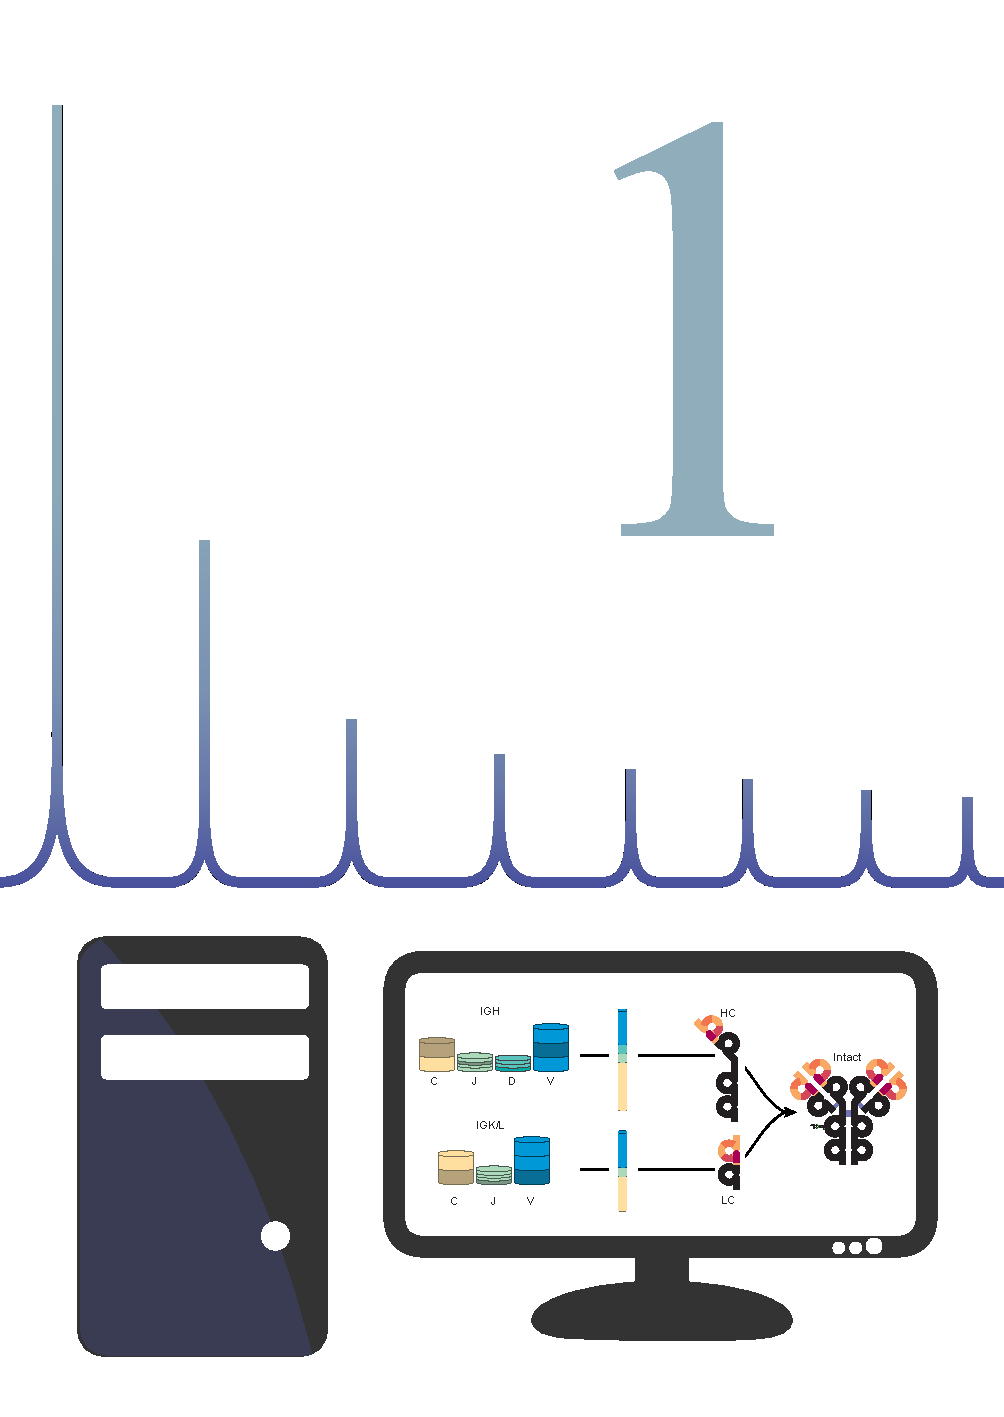
\includepdf{Chaptercovers/ch1.pdf} %add Chapter cover on blank page for 1st Chapter
\mainmatter % Begin numeric (1,2,3...) page numbering
\doublespacing % Double spacing
\numberedchapter
\picturechapterr{Introduction} \label{ch-1}

{
  \begin{center}
    \vspace*{0.5cm}
    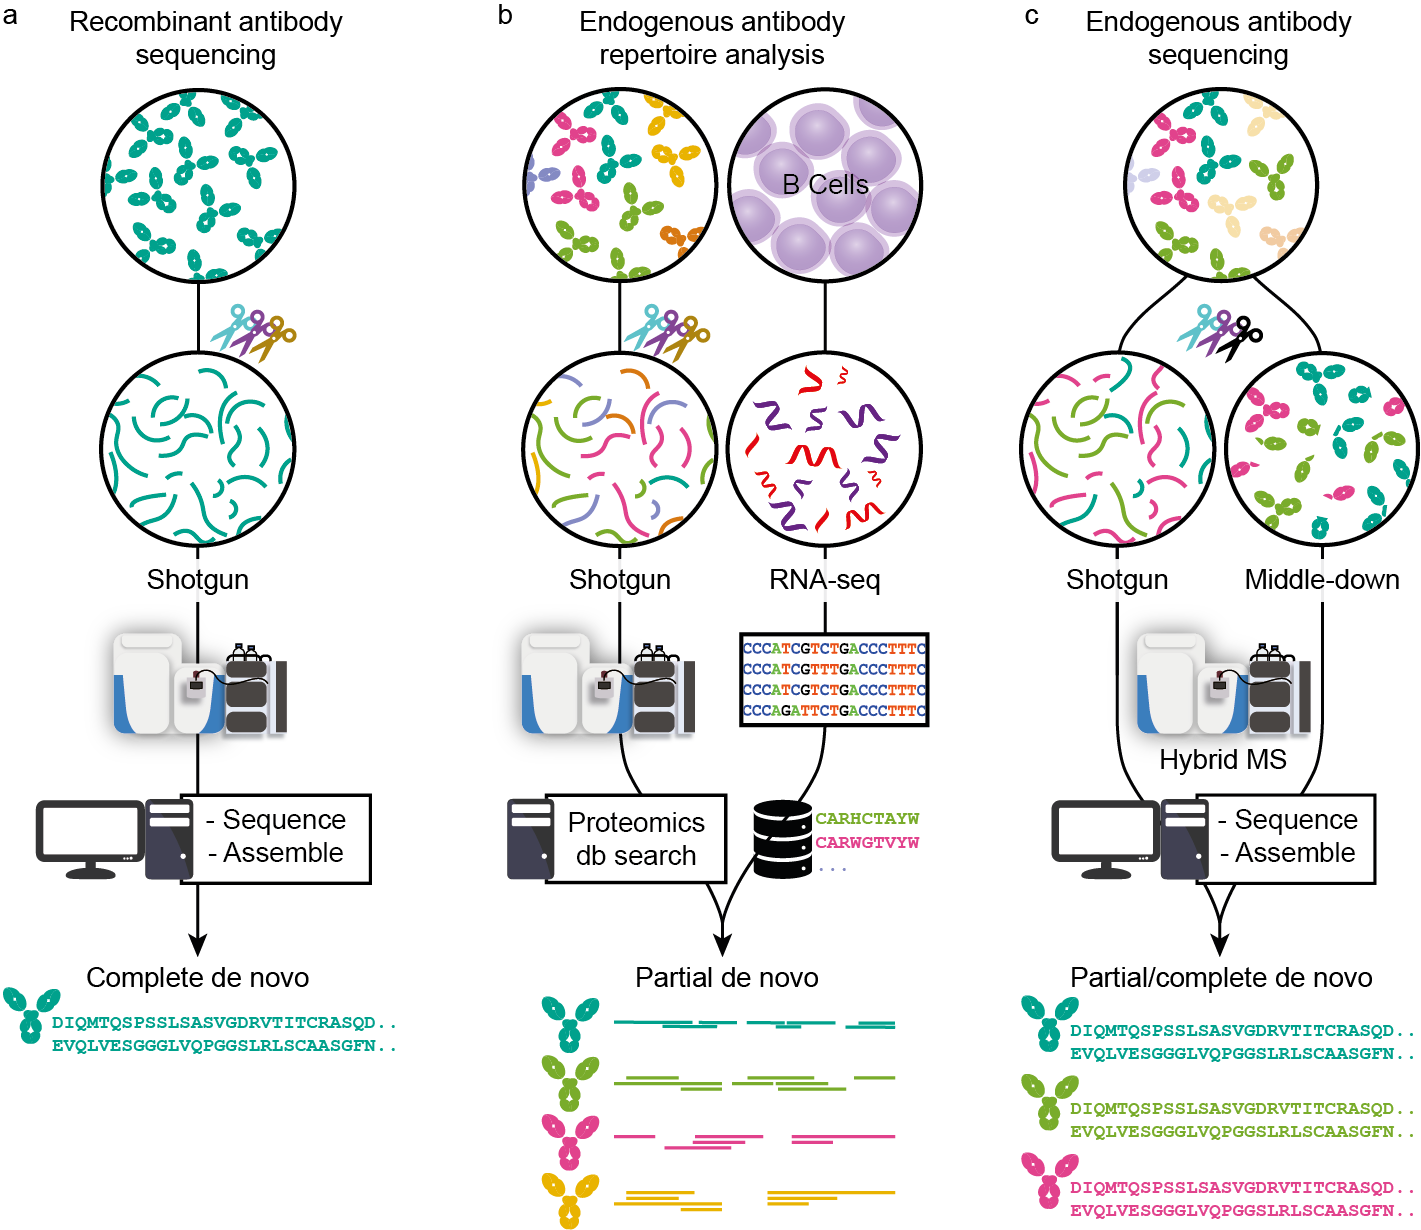
\includegraphics[]{Chapter.1/Figures/ch1.png}
    \vspace{0.25cm}
  \end{center}
}

\begin{flushleft}
  \vspace*{\fill}
  \rule{\textwidth}{1pt}\\[0cm]
  This chapter includes parts of the following publication:\\
  \textbf{A perspective towards mass-spectrometry-based \emph{de novo} sequencing of endogenous antibodies}\\
  \footnotesize
  \vspace{0.3cm}
  Sebastiaan C. de Graaf*, Max Hoek*, Sem Tamara and Albert J.R. Heck \\
  %%\vspace{0.3cm}
  \textbf{\emph{mAbs}} (2021), 14:1, 2079449, DOI: 10.1080/19420862.2022.2079449 \emph{Review}\\
  %%\footnotesize
  \vspace{0.3cm}
  \textsuperscript{*} These authors contributed equally to this work

\end{flushleft}
\newpage

\thumbforchapter

\section{Prelude - The importance of antibodies}
\lettrine[lraise=0.1, nindent=0em, slope=-.5em]{A}{round} the time of their initial discovery, antibodies were termed by various illustrious names, such as ‘Immunkörper’, ‘Amboceptor’, and ‘Zwischenkörper’, among many others. These terms were used more than a century ago to describe substances with antitoxin, lysin, agglutinin, and precipitin activities \cite{london1902der, lindenmann1984origin}. Nowadays, the generally accepted term \emph{antibody} refers to secreted immunoglobulins (Igs), whose sequence variety is several orders more diverse than the assortment of their historical names. Antibodies represent some of the most important molecules in the human immune system. Over the last century, Igs have been intensively studied because of their role in combatting infectious diseases and have taken centre stage for development of therapeutics in the last decade \cite{marks2020how, raybould2020thera-sabdab:, kaplon2021antibodies}. Beyond infectious diseases, recombinant antibodies are now also developed for cancer, rheumatoid arthritis, and various other pathological conditions \cite{singh2018monoclonal}. As key entities in the body’s defence mechanism, circulating antibodies are found in various bodily fluids, such as serum, saliva, milk, the lumen of the gut, and cerebrospinal fluid \cite{schroeder2010structure}. New leads for biotherapeutic development of recombinant antibodies come either from immunizing animals with specific antigens, or by discovering pathogen-neutralizing antibodies from recovered patients \cite{bornholdt2016isolation, corti2016protective, valgardsdottir2021identification}.
The estimated diversity of Ig molecules a human body can generate extends beyond 10\textsuperscript{15} theoretical sequences \cite{schroederjr.2006similarity, briney2019commonality}, indicating that each antigen may lead to a unique antibody response. These 10\textsuperscript{15} possible antibody sequences are all unique yet highly alike, posing a serious challenge for their characterization and sequencing, which has remained, to this day, a tremendously challenging task. Ideally, one would like to sequence antibodies at the protein level instead of through B-cell receptor (BCR) sequencing \cite{hom2022exploring}, as is currently the norm, to more directly probe circulating antibody repertoires and their relative abundances in specific environments. Mass spectrometry (MS) is expected to be the method of choice to potentially achieve this feat, as MS-based protein analysis has advanced and matured considerably \cite{altelaar2013next-generation, aebersold2016mass-spectrometric}. However, antibodies represent a very special and rather challenging class of proteins. Consequently, while MS has already been used to characterize and sequence highly purified monoclonal antibodies (mAbs) \cite{sen2017automated, peng2021mass, srzentić2020interlaboratory}, further technical developments in sample preparation and data analysis are needed to incorporate MS fully and efficiently into an endogenous humoral antibody discovery and characterization pipeline. In this thesis, I evaluate the role that MS can play in sequencing, identifying, and characterizing antibodies, focusing mainly on emerging strategies employed to enable identification and characterization of endogenous neutralizing antibodies.

\subsection{Nomenclature, structure, and diversity of antibodies}
Humoral human antibodies are complex proteins produced by B cells \cite{chiu2019antibody, schroeder2010structure}. Most antibody molecules (e.g. IgGs) are made up of four protein chains: two identical light chains and two identical heavy chains, which are interconnected by disulphide bridges (\textbf{\autoref{fig:fig1.1}}). The light and heavy chain form two heterodimers, which are connected via disulphide bridges in the hinge region to form the intact antibody. Functionally, the intact antibody can be divided into two antigen-binding domains (also known as Fab or fragment antigen-binding) and a constant domain (also known as Fc or fragment crystallizable) \cite{porter1959hydrolysis} (\textbf{\autoref{fig:fig1.1}a}). The Fc is the effector entity of the antibody and can bind to Fc-receptors on immune cells \cite{schroeder2010structure} and mediate immune effector responses such as phagocytosis, antibody-dependent cell-mediated cytotoxicity, respiratory burst, and cytokine release \cite{herr2003insights}. In contrast to the fully conserved sequence and structure of the Fc, the Fab is responsible for the vast diversity in recognized antigens and is thus hypervariable.
Because there is an endless and constantly evolving pool of pathogens, the antibody repertoire needs to be incredibly diverse and versatile to counteract these challenges \cite{charlesajaneway2001generation, alberts2002generation}. In humans, this enormous diversity in the potential antibody repertoire is achieved through several mechanisms. Starting at the genomic level, the light and heavy chains are encoded in four genes each: variable (V), diversity (D), joining (J), and constant (C), with the light chain lacking the D-gene. These genes are encoded in multiple alleles, which can recombine to a staggering number of combinations (\textbf{\autoref{fig:fig1.1}b}) \cite{jeske1984junctional}. The recombination process is also error-prone, leading to insertions and deletions at the junctions between the regions, referred to as junctional diversity. By recombination alone, the number of possible variable domain sequences already reaches tens of thousands. However, the eventual antibody diversity is expanded even further by natural polymorphisms, mutations, and class switching. As the major contributor to antibody hypervariability, somatic hypermutations can occur during B-cell affinity maturation and do so at a million-fold increased rate compared to the usual mutation rates \cite{schroederjr.2006similarity}. These mutations are largely concentrated in the complementarity-determining regions (CDR1-3), separated by framework regions (FR1-4), which form the conserved backbone of the Fab structure (\textbf{\autoref{fig:fig1.1}c}). Located at the tips of the Y-shaped antibody structure, CDRs are primarily responsible for antigen binding, and, therefore, elucidation of their sequences is of the utmost importance for antibody discovery.
\begin{figure*}[!htb]
  \center
  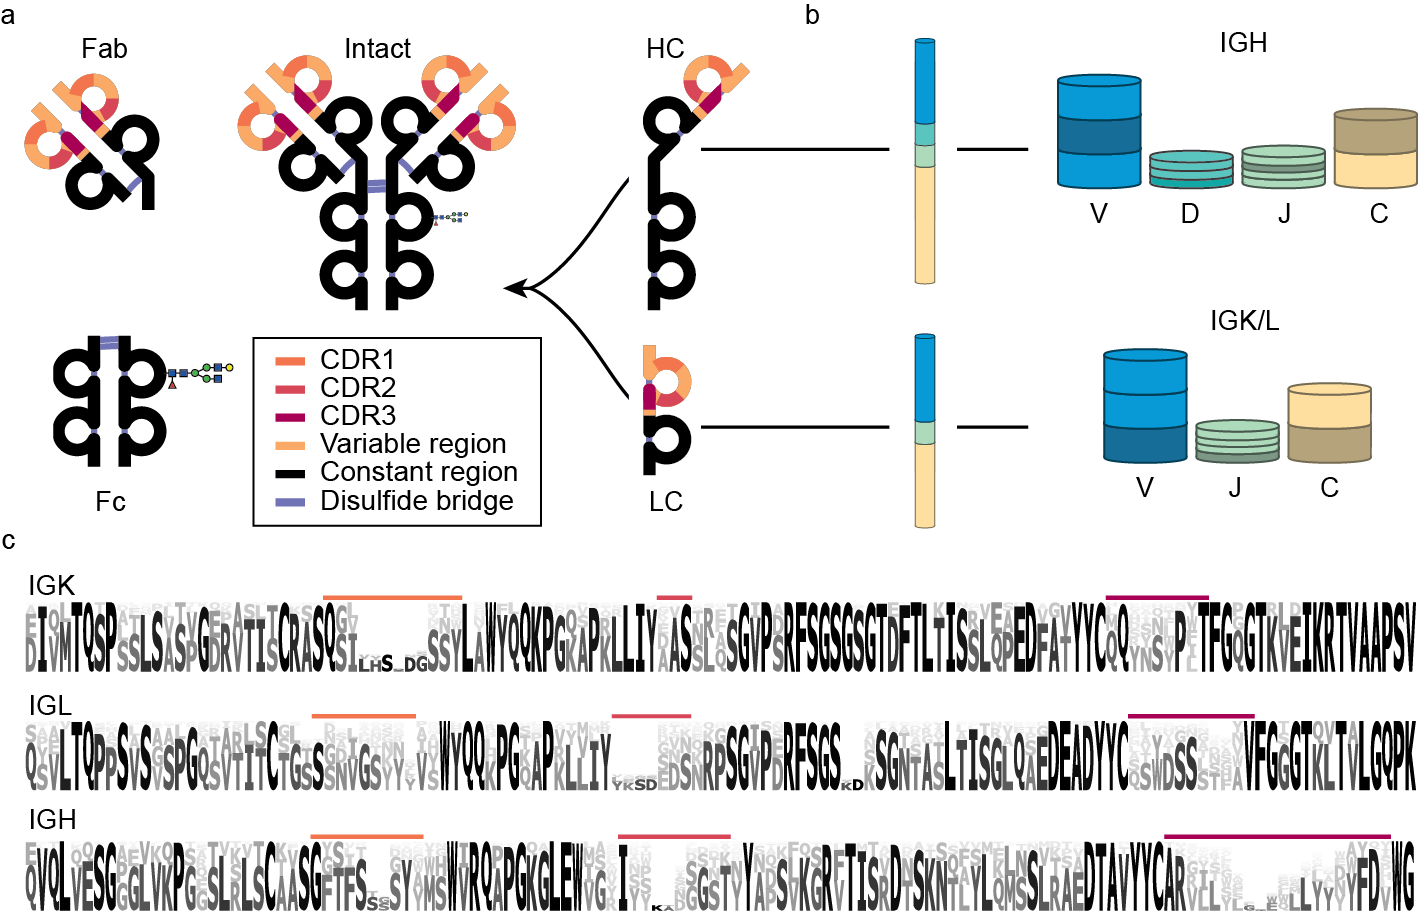
\includegraphics[]{Chapter.1/Figures/f1.png}
  \caption{
    \textbf{Nomenclature, structure, and diversity of IgG1 antibodies.}
    ~~a) Nomenclature and protein fragments of an IgG1 molecule. The antigen-binding domain, containing light and heavy chain (LC and HC respectively) variable regions, is termed Fab (or Fab2 when dimerized). The constant part of the heavy chain carrying an N-glycosylation site is called Fc. Other IgG subclasses vary in their heavy chain constant region (Fc) and disulphide patterns. ~~b) The diversity in antibodies originates primarily from the V, D, J, and C-allele (each annotated with a distinct colour) recombination process. In this process, each of many individual V, D, J, and C-alleles can recombine with any of the other gene segments, yielding thousands of possible combinations, in particular for the heavy chain, which incorporates the most diverse D region. ~~c) Sequence logo created by the alignment of in silico generated sequences of Ig kappa (IGK) and lambda (IGL) light chains and Ig heavy chain (IGH) from the international ImMunoGeneTics (IMGT) information system database \cite{lefranc2003imgt}. Even though the displayed sequences are part of the variable domain, large stretches of these sequences, also known as the framework regions (FRs), are relatively conserved, compared to the hypervariable complementarity determining regions (CDRs), coloured in accordance with ~~a) .
  }
  \label{fig:fig1.1}
\end{figure*}
The Fc part of Igs is used to classify antibodies into one of 5 classes: IgA, IgD, IgE, IgG, and IgM. Some of these classes are divided further into subclasses denoted by numbers, e.g., IgG1-4 or IgA1 and IgA2. Although the function of the classes and subclasses is different, their variable regions stem from the shared pool of genes. Therefore, for simplicity, in this review, we focus primarily on IgG1, the most abundant antibody subclass in serum, and the predominantly used subclass for biotherapeutic development. Still, concerning \emph{de novo} sequencing by MS, different Ig classes and subclasses pose similar challenges and opportunities.

\subsection{Modalities of MS-based antibody analysis}
Proteomics is the large-scale study of proteins. Many different peptide- and protein-centric MS-based approaches have been developed for proteomics, whereby some of these have been adapted for \emph{de novo} sequence analysis of antibodies.
Bottom-up (BU) or shotgun proteomics is by far the most widespread approach in MS-based protein analysis. In it, protein samples are digested by one or more proteases, and the resulting peptides are separated by some form of liquid chromatography (usually reversed-phase (RP)-HPLC), after which their peptide masses are recorded (MS1). Highly abundant precursor ions are then selected for fragmentation, and the masses of their fragment ions (MS2) are recorded.
Because digestion and MS-based fragmentation adhere to highly specific rules, peptides and their gas-phase fragment ions can be predicted. Consequently, peptides and their parent proteins are identified by comparing recorded spectra to the spectra simulated from protein or DNA databases \cite{aebersold2003mass}. For antibody sequencing, personalized databases are required for identification. Yet, digestion-based strategies are still widely used even without an available database. Individual spectra can be \emph{de novo} sequenced, and the resulting reads can be assembled into full-length sequences \cite{tran2016complete, guthals2012shotgun, sen2017automated}.
Additionally, intact mass analysis is a useful tool for protein analysis, providing masses that can be considered fingerprints of the species (known as proteoforms) present in the sample. Comparing different masses can lead to conclusions about relations between multiple species, for instance, if they differ by the mass of a known mutation, post-translational modification (PTM), or signal peptide \cite{donnelly2019best}. In the case of antibodies, such analysis can be performed with the protein in its native, and possibly complexed, state, or unfolded and separated into the comprising chains. Such approaches can provide valuable insights in the context of antibodies, e.g., by assessing the complexity of antibody repertoire or following changes in abundance of specific clones \cite{bondt2021human}. When applied to \emph{de novo} sequencing, the precursor mass knowledge can help determining the light and heavy chain pairing or sequence prediction accuracy in BU sequencing \cite{guthals2017de}.
In addition, both denatured and native antibodies can also be fragmented to yield some sequence information, this approach is called top-down (TD) MS. Because of the much larger size and higher charge of the analysed species, such intact-protein fragmentation spectra are more complex and harder to interpret than peptide spectra \cite{toby2016progress, compton2011on}. To mitigate this, specific proteases can be used to cleave proteins into smaller subunits. This practice is called middle-down (MD) MS, and in the context of antibodies it is often performed by cleaving the hinge region of the heavy chain before MS analysis \cite{johansson2008ides:}. Fragmentation spectra of entire chains or intact antibodies can provide valuable tools for both sequence determination and validation of sequence predictions, as fragmentation is highly specific for the precursor clone, which is often untrue in BU analysis \cite{fornelli2014middle-down}.

\section{The emerging role of mass spectrometry in antibody discovery}
Due to the structural complexity and immense sequence diversity of antibodies, the development of therapeutic antibodies has always been a very challenging and labour-intense task, especially when compared to small-molecule drug development. For example, the discovery of Trastuzumab was achieved by using mice immunized with antigen-expressing cells. Following the generation and selection of hybridomas that showed specific activity \cite{hudziak1989p}, the sequence of the selected antibody was determined after cloning and expression. A humanized antibody could be produced only thereafter by adapting and modifying the sequence accordingly \cite{carter1992humanization}. The same approach was used in the development of several other mAbs \cite{tsurushita2005design, khoja2015pembrolizumab, busse2001omalizumab, presta1993humanization}. Apart from being expensive and laborious, these early strategies required knowledge and availability of purified antigens and animal models that can produce specific antibodies in response to these antigens \cite{lu2020development}.
More recently, alternative strategies for antibody discovery have been explored starting with the screening of B cells from individuals who successfully overcame an infection. In this approach, peripheral blood mononuclear cells (PBMCs) are isolated, immortalized, and screened for antigen reactivity. The reactive clones are further expanded and characterized. This method has proven effective in finding new neutralizing antibodies that can be used to combat certain infectious diseases, e.g. Ebola \cite{bornholdt2016isolation, corti2016protective} or severe acute respiratory syndrome coronavirus 2 (SARS-CoV-2) \cite{valgardsdottir2021identification}. These recent advances show that the discovery of antibodies from human subjects, in addition to animal models, represents a viable method for developing new avenues for therapies. However, it may be even more advantageous to discover and characterize mature antibody clones directly from clinical samples at the protein level in their functionally matured and active form.
\begin{figure*}[!htb]
  \center
  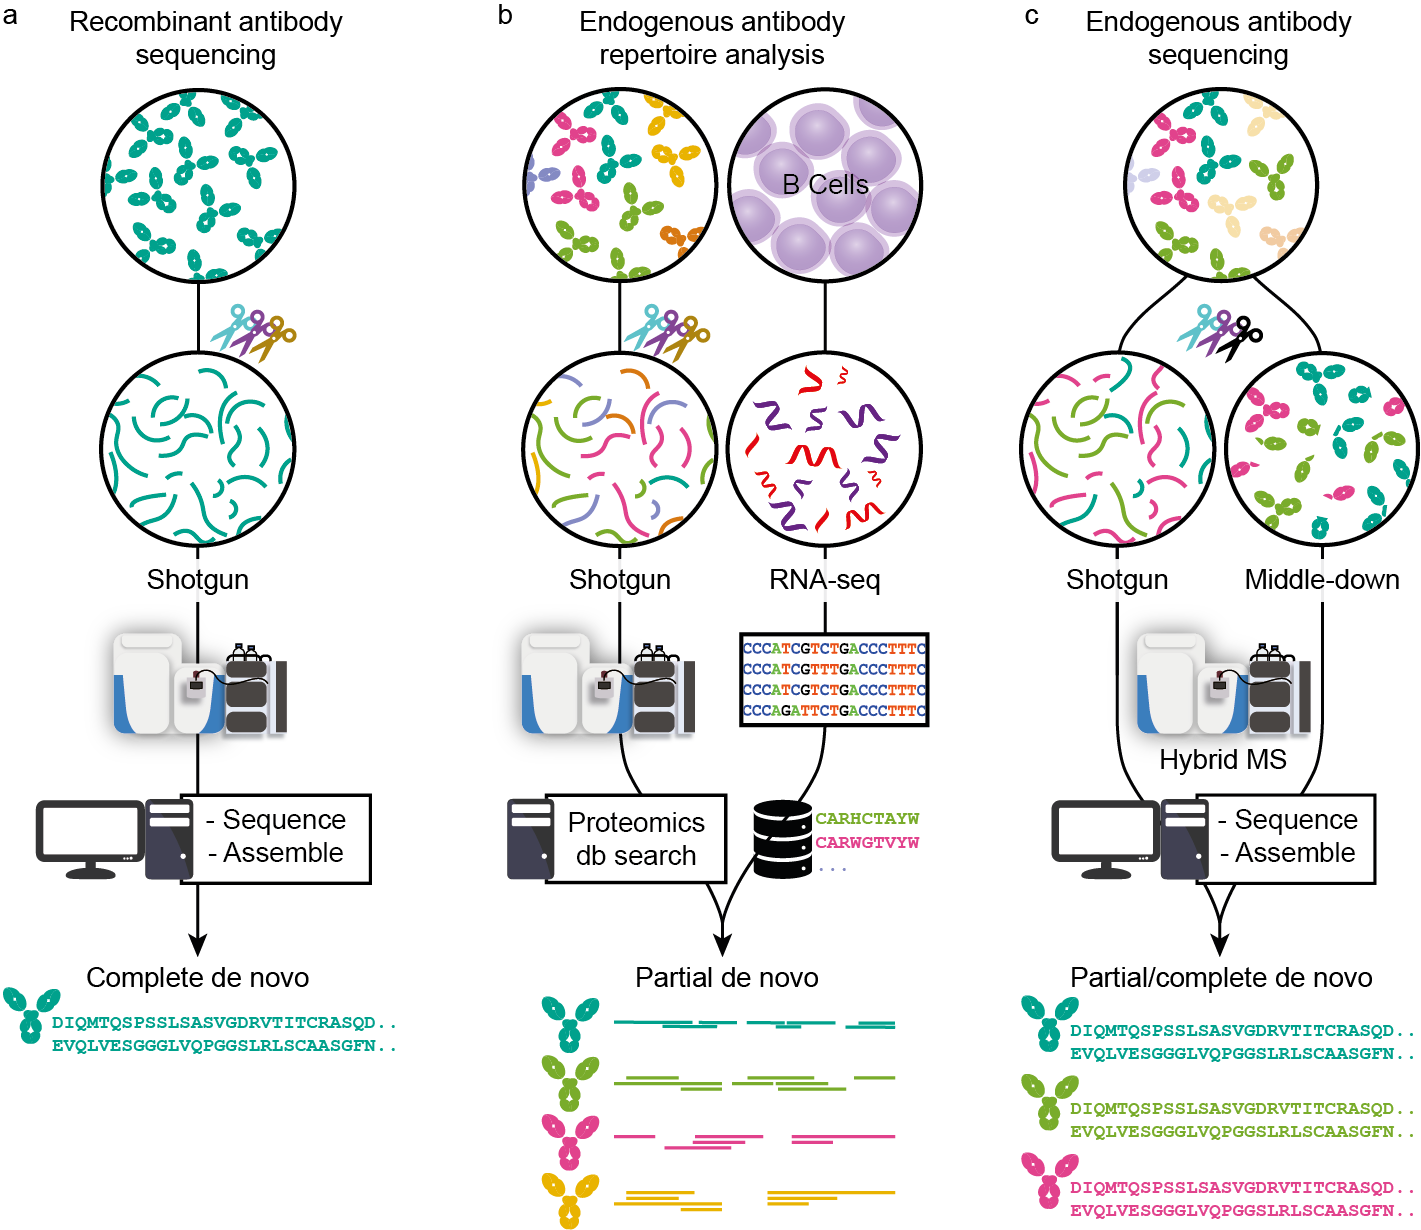
\includegraphics[]{Chapter.1/Figures/f2.png}
  \caption{
    \textbf{Three approaches in MS-based antibody sequencing.}
    ~~a) Recombinant antibody sequencing generally starts with abundant highly purified mAbs, which can be fully sequenced through BU MS, where hundreds of peptides are generated by digesting the mAb with one or several proteases, providing multiple overlapping short sequence reads. After liquid chromatography-mass spectrometry (LC-MS) measurement, the spectra can be processed by several different \emph{de novo} sequencing software solutions and assembled into full-length mAb sequences \cite{peng2021mass}. ~~b) In repertoire analysis, a sequence database is generated through B-cell sequencing, and MS-data is obtained through BU MS experiments. After generation of the personalized database, a high throughput of the LC-MS is possible \cite{georgiou2014promise}. While not strictly \emph{de novo} since only hits from the sequence database are identified, it is a powerful tool for antibody repertoire analysis. ~~c) Endogenous antibody sequencing cannot rely on BU MS alone, as direct sequencing of endogenous humoral antibodies is hampered by inherent challenges and complexity. Emerging MD and TD MS techniques provide clone-specific sequence information highly complementary to traditional sequencing. Integrating BU MS and MD/TD MS makes it possible to achieve full-length coverage of antibody sequences \cite{bondt2021human}.
  }
  \label{fig:fig1.2}
\end{figure*}

In recent years, MS-based proteomics has advanced tremendously in sample preparation, MS and liquid chromatography instrumentation, and data analysis \cite{altelaar2013next-generation, aebersold2016mass-spectrometric}. Using all these advances, antibody sequencing at the protein level by MS has come within reach. \textbf{\autoref{fig:fig1.2}} highlights three – chiefly MS-based – strategies used to determine antibody sequences. These three pillars are primarily classified by the source of sample material and the attainable sequencing information. The first strategy applies to highly purified recombinant antibodies that are now amenable for full sequencing with BU MS, often by combining several different proteases and advanced algorithms. Second, hybrid approaches have been introduced for analysing endogenous antibody repertoires by combining MS-based techniques with genomics or transcriptomics, e.g., whole genome sequencing or BCR sequencing, ideally from the same donor. The third set of techniques encompasses several MS-based \emph{de novo} approaches that aim to determine complete antibody sequences of selected clones directly from clinical samples without the aid from alternative omics data. While each strategy is distinct, they all share common aspects.


\subsection{MS-based sequencing of monoclonal antibodies}
Before delving into the topic of MS-based sequencing of endogenous antibodies from clinical samples, we first discuss the current state-of-the-art sequencing approaches developed for recombinant mAbs. Principles of mAb sequencing by MS share many technical considerations with sequencing of antibodies present in complex mixtures. Furthermore, currently available strategies for recombinant mAb sequencing provide great context for discussing limitations and bottlenecks that hamper sequencing of endogenous antibody clones.

\subsubsection{Shotgun, bottom-up strategies used for sequencing of highly purified mAbs}
Antibodies are often analysed after digestion with one or more proteases to generate peptides (\textbf{\autoref{fig:fig1.2}}). Such peptide-centric approaches are known as BU MS and represent the most popular type of proteomics experiments. In contrast to most shotgun proteomics experiments, \emph{de novo} sequencing through BU MS necessitates a high depth of sequence coverage, i.e. each sequence position in the antibody is ideally supported by multiple overlapping unique peptides. With a typical highly specific protease such as trypsin, which cleaves C-terminally of lysine and arginine, and a low number of missed cleavages, sequence-coverage depth is often limited because only a few of the generated peptides overlap in sequence. Although this suits standard shotgun proteomics experiments, which do not require full sequence coverage of the analysed proteins, \emph{de novo} sequencing of antibodies thus requires other approaches.
Several methods to generate complete and deep sequence coverage by overlapping peptides have been introduced. For example, a shortened protease incubation time was successfully used to increase the number of peptides carrying missed cleavage sites \cite{morsa2019multi-enzymatic}. Some proteases generate a high number of overlapping peptides through non-specific cleavage \cite{bandeira2008beyond, castellana2010template, guthals2017de}. Alternatively, non-specific cleavage can be also achieved through non-enzymatic treatment, e.g., microwave-assisted hydrolysis \cite{savidor2017database-independent}. For these methods to work, digestion conditions must be tightly controlled to avoid abnormally long or short peptides and ensure reproducibility. Another elegant option is to use multiple proteases with synergistic sequence specificities. For instance, Peng et al. \cite{peng2021mass} recently used a total of 9 proteases, both specific and non-specific, to successfully \emph{de novo} sequence a full-length anti-FLAG-M2 mouse mAb (\textbf{\autoref{fig:fig1.3}}). The strength of a large panel of proteases is shown in the validation of the CDR sequences by high scoring peptides covering the entire CDR. The 6 chosen peptides are the result of digestion by 5 different proteases (trypsin, chymotrypsin, lysC, thermolysin, and elastase, \textbf{\autoref{fig:fig1.3}a and b}).
Nowadays, most \emph{de novo} sequencing solutions, such as ALPS/PeaksAB \cite{tran2016complete}, GenoMS \cite{castellana2010template}, SuperNovo \cite{sen2017automated} and Champs \cite{liu2009automated} are quite successful in obtaining full sequence coverage of highly purified antibodies. To determine the antibody sequences \emph{de novo}, all these software tools require large number of overlapping peptides, spanning the entire sequence, which are successfully fragmented and converted into predicted peptide sequence reads (\textbf{\autoref{fig:fig1.2}a}). This necessitates generation of BU MS data by using multiple proteases. While complicating sample preparation and increasing the required amount, such multi-protease approaches are advantageous for \emph{de novo} sequencing by alleviating the sequence assembly problem.
\begin{figure*}[!htb]
  \center
  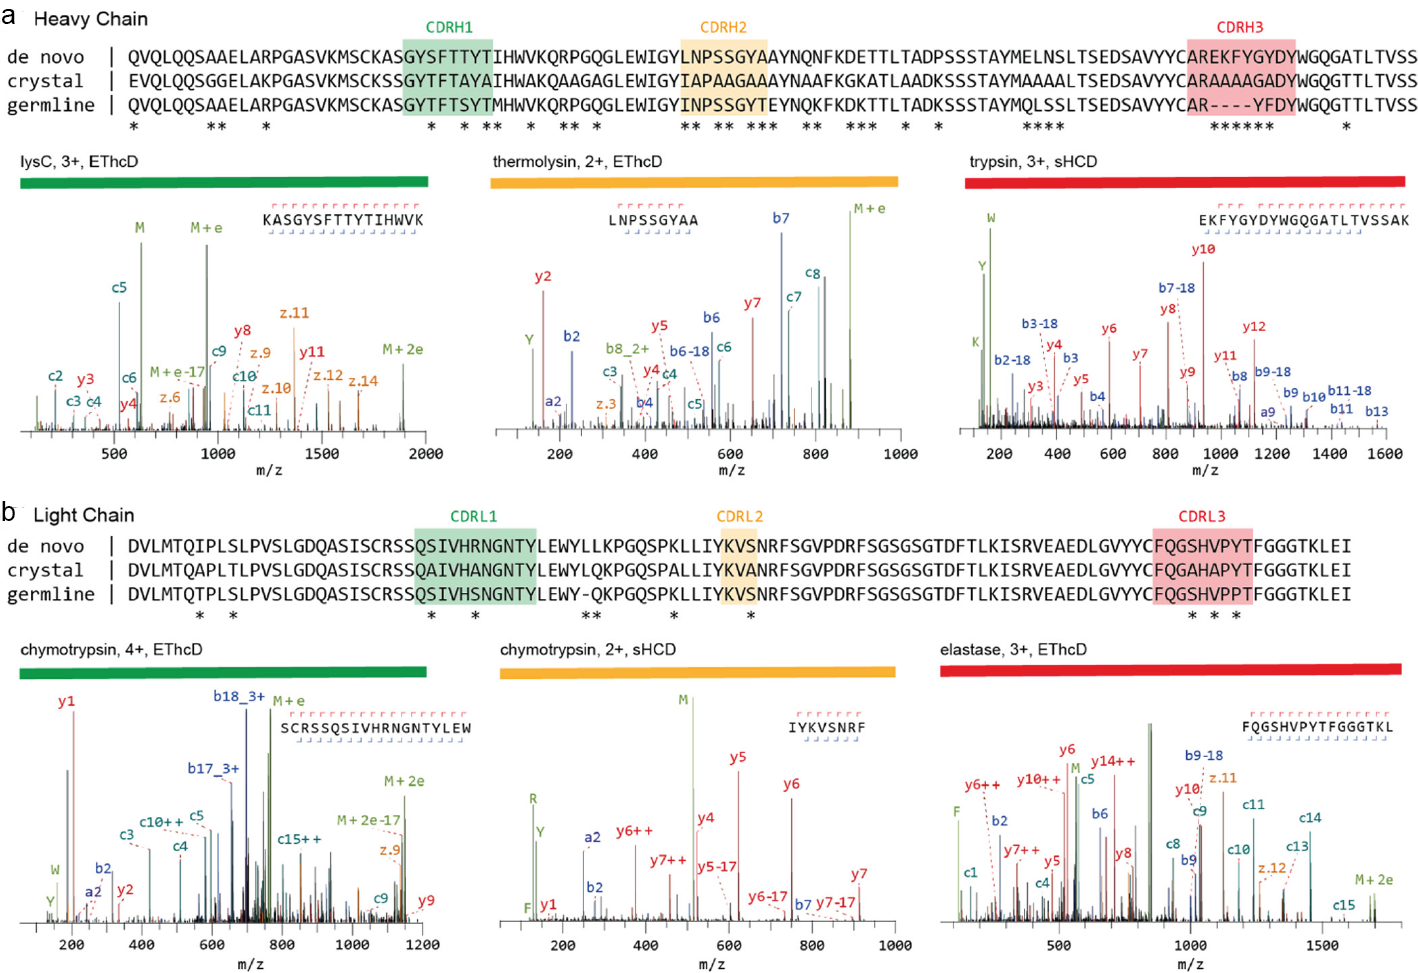
\includegraphics[]{Chapter.1/Figures/f3.png}
  \caption{
    \textbf{Sequencing of a monoclonal Anti-FLAG M2 antibody.} The variable regions of the heavy ~~a) and light chains ~~b) are shown. The \emph{de novo} sequence derived by MS is shown on top, alongside the previously published sequence used in the crystal structure of the Fab (PDB ID: 2G60), and germline sequence (IMGT-DomainGapAlign; IGHV1-04/IGHJ2; IGKV1-11$\star$7/IGKJ1). Differential residues are highlighted by asterisks (*). Exemplary MS/MS spectra in support of the assigned sequences are shown below the alignments, labelled with protease, precursor charge state, and fragmentation type. The peptide sequence and fragment coverage are indicated in the top-right of each spectrum spectra, with \emph{b/c} ions indicated in blue/teal and \emph{y/z} ions in red/orange. The same colour annotation is used for peaks in the spectra, with additional peaks such as intact/charge reduced precursors, neutral losses, and immonium ions indicated in green. To prevent overlapping peak labels, only a subset of successfully matched peaks are annotated. Figure and caption adapted from Peng et al. \cite{peng2021mass}
  }
  \label{fig:fig1.3}
\end{figure*}


\subsubsection{Benefits of complementary peptide fragmentation techniques}
In MS-based sequencing, extensive fragmentation of peptide ions is essential to generate arrays of adjacent fragments that reveal the amino acid sequence, often referred to as ion ladders or sequence tags (\textbf{\autoref{fig:fig1.4}a}). The amino acid sequence of the fragmented peptide is derived by comparing the mass difference between two adjacent fragment ion peaks to the masses of amino acids and combinations thereof. The produced fragment ion series must contain very few gaps larger than a single amino acid residue, because such gaps lead to exponential growth of the amino acid combinations that fit the mass difference, particularly for spectra of lower resolution \cite{he2018protein}. Since there is no universal fragmentation method that can produce uninterrupted fragment ion ladders for all possible peptides, it is highly advantageous to use various fragmentation methods with distinct mechanisms and specificities to complement each other (\textbf{\autoref{fig:fig1.4}b}) \cite{macias2020ion}. While collisional dissociation (CID/CAD/HCD) is the most used technique in shotgun proteomics experiments, multiple alternative fragmentation techniques have been introduced and have proven to be complementary. These specificities stem from the unique ion activation mechanisms employed by each method. In collision-based techniques, energy is deposited to the multiply protonated peptide ions through low-energetic collisions with inert neutral atoms or gas molecules. This energy is redistributed vibrationally throughout the peptide backbone, fragmenting the most labile bonds and yielding \emph{b/y}-type fragment ions, as defined by the Roepstorff-Fohlmann-Biemann ion nomenclature (\textbf{\autoref{fig:fig1.4}c}) \cite{roepstorff1984proposal}. Although protonated amide bonds are usually the most susceptible to fragmentation, collisional dissociation often also leads to loss of labile PTMs, such as phosphorylation and sialyation.
\begin{figure*}[!htb]
  \center
  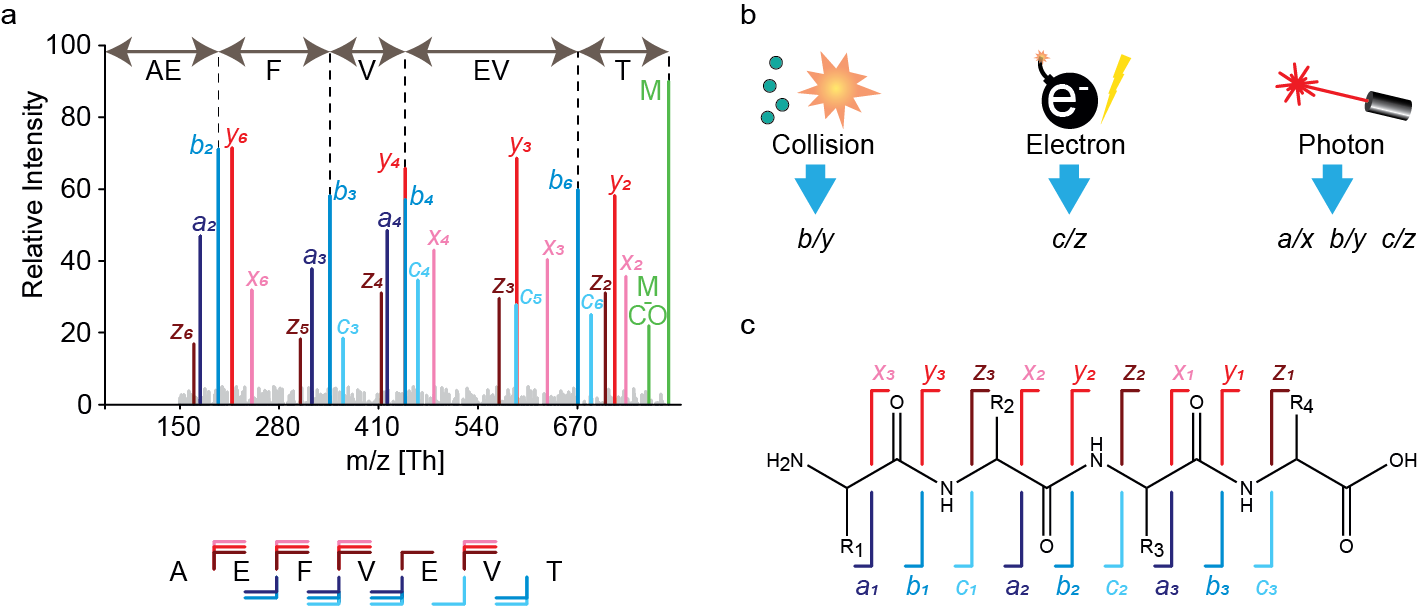
\includegraphics[]{Chapter.1/Figures/f4.png}
  \caption{
    \textbf{Peptide fragmentation in MS-based \emph{de novo} sequencing.} ~~a) An illustrative fragmentation spectrum. In the spectrum, fragment ion peaks are colour annotated according to the type of fragment ion (\emph{a}: purple, \emph{b}: blue, \emph{c}: light blue, \emph{x}: pink, \emph{y}: red, and \emph{z}: brown) the unfragmented peptide (precursor ion) is shown in green as well as the precursor ion with neutral loss of CO. Adjacent fragment ions of the same type have a mass difference corresponding to a single amino acid, which is used to determine the sequence as is illustrated for \emph{b}-ions above spectrum. Below the spectrum the amino acid sequence is shown together with the fragment ion annotation, N-terminal fragments (\emph{a-, b- ,c-}) are below the sequence and C-terminal fragments (\emph{x-, y-, z-}) are shown above the sequence. ~~b) Three predominant gas phase fragmentation techniques with their predominantly produced fragment ion types. Collisional dissociation (CID/CAD/HCD) predominantly yield \emph{b/y} ions. Electron based dissociation (ECD/ETD) yields \emph{c/z} ions. Contrary the other techniques, high energy photon based dissociation (UVPD) results in all fragment ion types \cite{brodbelt2016ion}. ~~c) The Roepstorff-Fohlmann-Biemann nomenclature used for peptide fragment ions denotes different fragment ion types by italic letters \emph{a-c} and \emph{x-z}. The numbering indicates the position of the bond in the amino acid sequence with respect to the N- and C-termini.
  }
  \label{fig:fig1.4}
\end{figure*}
In electron-based techniques (ECD/ETD), positively-charged peptide ions capture electrons, leading to the generation of odd-electron species that dissociate promptly without significant vibrational redistribution \cite{syka2004peptide, zubarev2000electron, mcluckey1998ion/ion}. In contrast to collisional dissociation, this process is not directed towards the most labile bonds, and produces distinctively \emph{c} and \emph{z} fragment ions through the dissociation of N-Cα bond (\textbf{\autoref{fig:fig1.4}c}). Similarly, high-energy photon-based activation techniques (UVPD) also cause bond dissociation without substantial energy redistribution. This is enabled by a number of chromophores along the peptide backbone and results in a wide array of co-occurring fragment ion types (\emph{a/x, b/y, c/z}), depending on the wavelength used \cite{brodbelt2016ion, brodbelt2020ultraviolet}. Highly energetic fragmentation methods can also lead to \emph{w}-type ions, which involve an amino acid side chain dissociation \cite{xiao2016distinguishing, kjeldsen2003distinguishing}. In \emph{de novo} sequencing, this may be advantageous since it allows to distinguish between leucine and isoleucine, which are commonly misassigned because they have an identical mass.
While having multiple fragment ion types in a single spectrum can complicate ion ladder detection (\textbf{\autoref{fig:fig1.4}a}), it can also provide insight into the direction of fragment ion series, revealing to which terminus (N or C) peptide fragments belong. This is possible due to the characteristic mass shift patterns of consecutive \emph{a, b, c} fragments and consecutive \emph{x, y, z} fragments originating from the same peptide bond. Horn et al. \cite{horn2000automated} pioneered this approach for \emph{de novo} protein sequencing by combining CID and ECD to discern between the N- and C-terminal fragment ions, which simplified the detection of consecutive fragment ions. Subsequently, many others have used similar strategies \cite{guthals2013sequencing-grade, vyatkina2017de, datta2009spectrum, horton2017comprehensive, bertsch2009de}.
The previously described publication by Peng et al. \cite{peng2021mass} also demonstrates the successful application of using multiple fragmentation techniques. They recorded spectra using a dual fragmentation scheme of both high-energy collision dissociation (HCD) and electron-transfer high-energy collision dissociation (EThcD), resulting in a reduced number of sequencing errors when compared to using a single fragmentation method. The spectra selected to support the CDR predictions are also derived from both fragmentation techniques, showing that this versatile fragmentation strategy can benefit sequence coverage in these challenging and important regions (\textbf{\autoref{fig:fig1.3}}).
Such multiplexing MS strategies have made \emph{de novo} sequencing of mAbs feasible, at least when they are of sufficient purity. However, the procedure is quite laborious as it often involves using multiple proteases to generate overlapping peptides and multiple peptide fragmentation techniques to obtain unambiguous sequence reads, which entails longer sample preparation time, the requirement of larger sample amounts, and extensive data acquisition.

\subsubsection{Homology-aided \emph{de novo} sequencing of antibodies}
To identify peptides and proteins, shotgun proteomics experiments rely on matching observed fragmentation spectra to theoretical spectra generated from sequence databases. However, complete and accurate mature sequences are not generally available for many proteins, especially for highly variable or frequently mutated proteins like antibodies. Instead, homologous sequences, primarily derived from genomic or transcriptomic experiments, can be used. For antibodies, the genes encoding for each of the regions (V, D, J, and C) are available as germline sequences and can be retrieved from the IMGT database \cite{lefranc2003imgt, lefranc2020immunoglobulins}. While such a database of homologous sequences can facilitate verification or guide predictions of \emph{de novo} sequences, it should be noted that the exact match to the target sequence is likely not present even in the most extensive databases. Traditional database searches are thus not applicable because they require exact mass matching of fragments, and a single amino acid mutation can prevent identification. Instead, error-tolerant fragment matching algorithms, either based on sequence alignments or subsequence (i.e., sequence tag) extractions, can use homologous databases to score experimentally determined sequences.
An example of a homology-aided approach is searching BU MS data from a sample of human antibodies against a proteome database such as Swiss-Prot, whereafter the identified peptides are aligned to the IMGT database \cite{schmelter2017peptides, singh2013cerebrospinal-fluid-derived}. Further reported adaptations include \emph{de novo} sequencing of unidentified features from the initial search with dedicated tools, such as PEAKS, to sequence and identify hypervariable regions \cite{broodman2012mass, costa2010sequencing}. Homology-aided \emph{de novo} sequencing algorithms are also advantageous in identifying erroneous \emph{de novo} peptide reads by comparing them against homologous sequences. In addition, they can be used as a germline template to aid in the assembly of \emph{de novo} peptide reads. Alternative to scaffolds based on homologous sequences, accurate masses of the antibody clones and constituent parts, e.g., light chain or heavy chain, can create mass-based scaffolds. However, these masses need to be obtained separately by performing additional protein-centric MS experiments.

\subsubsection{Protein-centric MS approaches}
Although conventional \emph{de novo} sequencing of proteins predominantly follows a peptide-centric approach, there have been various attempts to analyse recombinant mAbs intact or at the level of large domains, e.g., Fabs, bringing along a new set of challenges. First, compared to peptides, intact proteins sometimes ionize less efficiently, and liquid-chromatography-based separation of peptides is more established and efficient than separation of intact proteins. Furthermore, in MS analysis, mass accuracy and resolution typically diminish with increasing molecular weight, even when using the latest high-resolution mass spectrometers \cite{tamara2021high-resolution, donnelly2019best, lössl2014boundaries}. In addition, full sequence coverage is generally unattainable for intact proteins with masses above 20 kDa. These factors have significantly held back the implementation of protein-centric MS for \emph{de novo} sequencing of antibodies. However, more recently, several advances in the field resulted in relatively high sequence coverages, reported for recombinant mAbs with available reference sequences \cite{fornelli2014middle-down, mao2013top-down, tsybin2011structural, resemann2016full}. Protein-centric approaches, termed TD MS \cite{toby2016progress}, can provide additional valuable information, including the mass of the intact antibody \cite{donnelly2019best}, masses of the light and heavy chains, and some predictable fragment ions, which could be used as mass constraints \cite{bondt2021human, greisch2021generating, boer2020selectivity, greisch2021extending, srzentić2020interlaboratory}.
Similar to peptide-centric strategies, there is the potential to combine multiple fragmentation techniques in TD MS to boost sequence coverage. In addition, intact antibody sequencing can be simplified by reducing the complexity and size of the antibody through disulphide reduction or by digestion of the antibodies using specific proteases, such as IgdE (commercially termed FabALACTICA), which cleaves above the hinge region of IgG1, specifically producing 50 kDa Fab fragments \cite{spoerry2016identification}, or IdeS (FabRICATOR), a cysteine protease that digests antibodies at a specific site below the hinge, generating F(ab’)2 fragments of all IgG subclasses \cite{johansson2008ides:}. Such strategies deviate from intact protein sequencing, which resulted in the introduction of the term MD MS \cite{lermyte2019top}. However, these MD strategies still adhere to the core principles of protein-centric MS, whereby large (50-100 kDa) domains of antibodies are analysed.
In a large body of works, Fornelli et al. \cite{fornelli2012analysis, fornelli2014middle-down, fornelli2017top-down, fornelli2018accurate} have shown how various factors, including sample preparation strategies, fragmentation conditions, and other improvements in instrumentation and experimental design, influence sequence coverage in the protein-centric analysis of recombinant mAbs. Recently, Shaw et al. \cite{shaw2020direct} demonstrated that with modern instrumentation it is possible to successfully fragment intact mAbs in their native state (\textbf{\autoref{fig:fig1.5}}). By combining ECD and HCD in a single tandem MS experiment, 42\% sequence coverage for the light chain (\textbf{\autoref{fig:fig1.5}a}) and 20\% sequence coverage for the heavy chain (\textbf{\autoref{fig:fig1.5}b}) of Trastuzumab were obtained. The resulting fragmentation spectrum contained not only the multiply charged backbone fragmentation products but also the intact light chain, ejected from the antibody by fragmentation of the intermolecular disulphide bridge, providing information on the light and heavy chain pairing (\textbf{\autoref{fig:fig1.5}c}). These and many other studies culminated in a large joint effort by the Consortium for Top-Down Proteomics, wherein they comprehensively described available approaches, techniques, and instrumentation for the analysis of recombinant mAbs \cite{srzentić2020interlaboratory}.
Electron-based fragmentation of intact protein ions holds great potential for mAb sequencing. Several recent studies showed that these methods consistently yielded nearly uninterrupted \emph{c}-ion ladders spanning the CDR3, which is paramount to antigen binding \cite{boer2020selectivity, greisch2021generating, bondt2021human, shaw2018sequencing, shaw2020direct}. These studies also demonstrated for various antibody subclasses (IgG1-4 and IgA1) that electron-based fragmentation methods consistently provide fragments containing the entire variable region of both the light and heavy chain. Notably, very similar fragments were formed for the intact mAb, the F(ab’)2 (produced with IdeS enzyme), and Fab molecules (produced with IgdE or Operator enzymes), showing that reducing antibody complexity through the removal of the Fc portion is not detrimental for protein-centric analysis of mAbs.
While significant advances have been made in protein-centric sequencing of purified recombinant antibodies, studying endogenous antibodies remains much more challenging. The separation of intact proteins by liquid chromatography is typically less efficient than the separation strategies available for peptides \cite{shen2017high-resolution}. This problem is exacerbated for antibody mixtures since different antibody clones are very similar and only vary in a small fraction of the overall sequence. Such minute differences are easily resolved on the peptide yet are significantly more difficult to distinguish on the level of intact antibodies with more than 1000 amino acid residues. Notwithstanding the challenges of intact protein MS, the prospects and potential benefits that protein-centric approaches bring to the \emph{de novo} analytical toolbox are hard to neglect. While it is still nearly impossible to fully \emph{de novo} sequence intact mAbs, protein-centric sequencing can be combined with peptide-centric methods in a hybrid MS approach, providing complementary information substantially advancing towards the goal of complete antibody sequencing by MS, as further described in the section “Combining peptide- and protein-centric MS approaches for antibody sequencing” (\textbf{\autoref{fig:fig1.2}b}).
\begin{figure*}[!htb]
  \center
  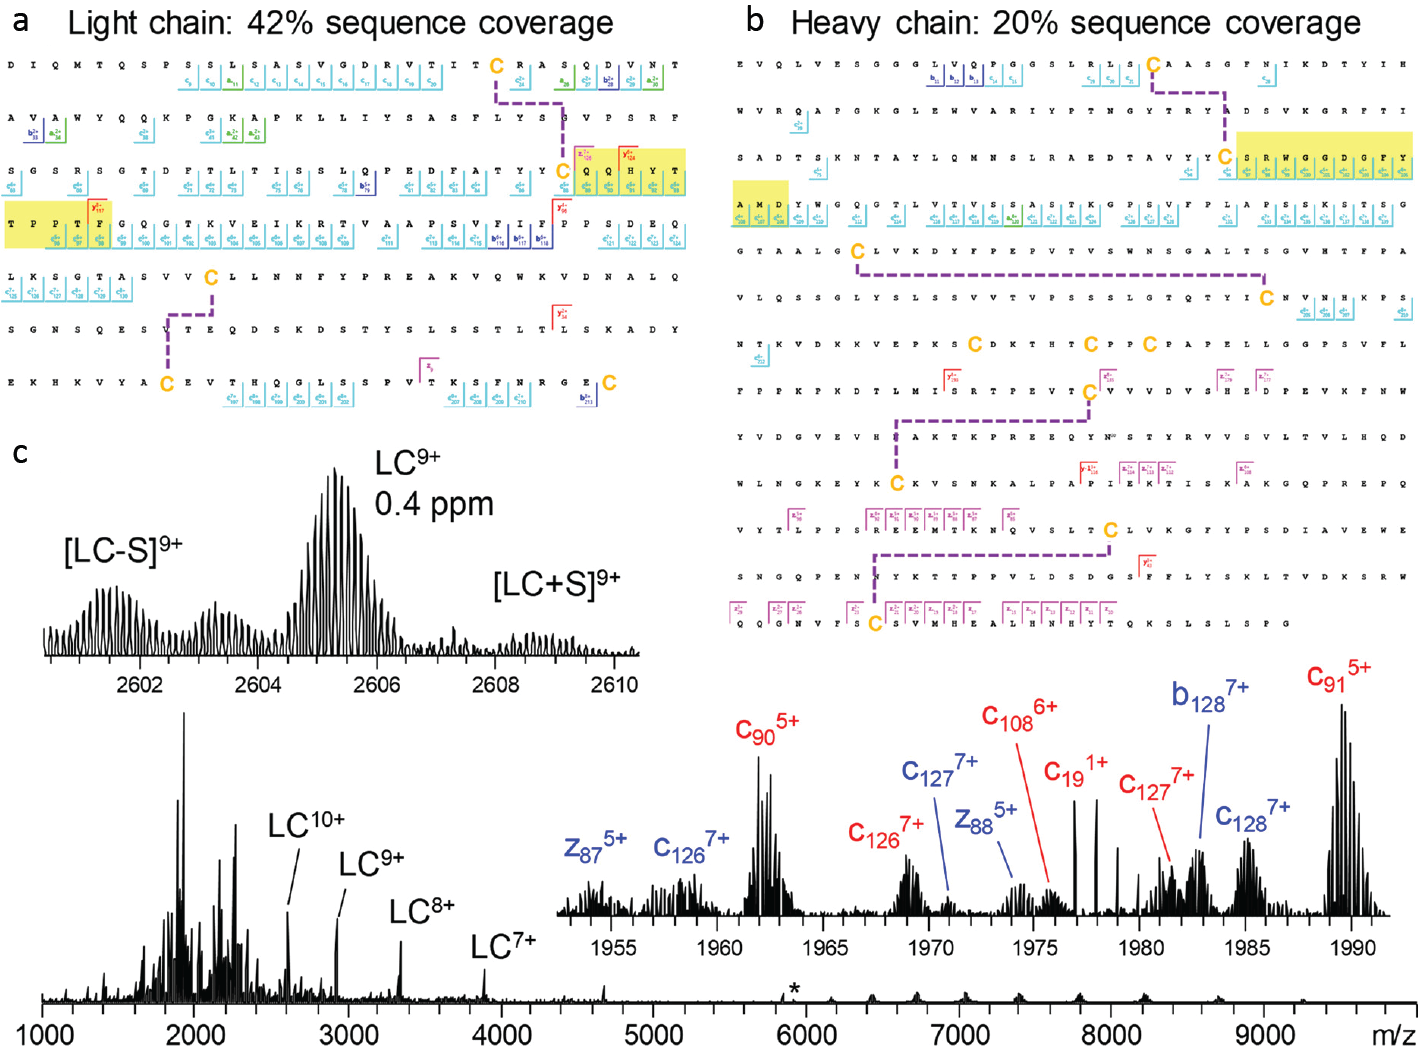
\includegraphics[]{Chapter.1/Figures/f5.png}
  \caption{
    \textbf{Light chain ~~a) and glycosylated heavy chain ~~b) fragmentation maps illustrate sequence coverage produced by the combination of ECD and HCD on Trastuzumab.} Disulphide bonds are shown by dashed lines, CDR3 regions are highlighted in yellow. The corresponding fragmentation spectrum ~~c) for the 25+ charge state of intact Trastuzumab with insets displaying the zoomed in region containing the 9+ charge state of the light chain and various fragment ions. Red and blue fragment ion labels correspond to the light and heavy chain, respectively. Asterisk indicates the mass-selected precursor ion. Figure adapted from Shaw et al. \cite{shaw2020direct}
  }
  \label{fig:fig1.5}
\end{figure*}


\subsubsection{Dedicated software solutions for MS-based antibody sequencing}
The various sample preparation methods and intricate experimental designs presented above result in extended datasets that are not feasible for manual interpretation. Thus, development of dedicated software tools for data interpretation is essential.
With regards to BU MS data, presently, two popular software suites are tailored towards \emph{de novo} sequencing of antibodies, SuperNovo \cite{sen2017automated} and PeaksAB \cite{tran2016complete, ma2003peaks:}. These suites can utilize the benefits of data generated by using multiple enzymes, multiple fragmentation methods, and the use of a homologous antibody germline sequence database like IMGT to make a complete \emph{de novo} sequence prediction based on the BU MS data. More specifically, the software iteratively screens predicted peptides against the germline gene segments of the antibody to determine the positions on the final chain construct. Homologous germline sequence candidates represent scaffolds that are then modified to account for the highest scoring predicted peptides. This allows for predicting both heavy and light chain sequences with a minimal error rate of only a few single amino acids per sequenced antibody. A downside, however, is that the software works so far exclusively for sequencing single, highly purified antibodies.
Novel software solutions for \emph{de novo} antibody sequencing are emerging and advancing in parallel with improvements in experimental design and instrumentation. The fast development of new \emph{de novo} sequencing strategies encourages the development of new software solutions and improvement of already established tools and requires adaptable software to accommodate the frequent and considerable shifts in \emph{de novo} sequencing approaches, such as the inclusion of TD or MD MS data, multiple fragmentation methods or the analysis of polyclonal samples as opposed to mAbs.

\subsubsection{Combining peptide- and protein-centric MS approaches for antibody sequencing}
Recent advances in protein-centric MS have spawned various software tools that use these data either in a standalone manner, such as in Twister \cite{vyatkina2015de, vyatkina2017de}, or integrate them with BU MS data, as in TBNovo \cite{liu2014de}. Twister applies methods similar to those used for BU MS sequencing, recombining individual sequence tags (rather than peptide reads) into longer sequences using a specific implementation of de Bruijn graphs (T-Bruijn graphs) and sequence tag convolution \cite{vyatkina2015de, vyatkina2017de}. TBNovo uses sequence tags and precursor masses from TD MS to provide a scaffold for positioning the \emph{de novo} predicted peptide reads to fill the complete sequence. Their analysis makes use of external BU \emph{de novo} sequencing software, PEAKS \cite{ma2003peaks:}, and was tested on protein mixtures. TBNovo has not achieved widespread adoption, perhaps due to the software’s complexity and because protein-centric MS was still barely practiced at the time of its first release.
Although antibody sequencing at the protein level is still not trivial, it is being applied on a steadily increasing scale in academia and industry. Efforts to extend the sequencing of antibodies to polyclonal mixtures have however proven extremely challenging. The first obstacle is sample availability. While recombinant mAb samples are typically available in milligram quantities, polyclonal antibody samples are often derived from clinical samples and thus will only be available in limited quantities. Because the median concentration of individual clones in plasma is $\sim$1 µg/mL the available protein per individual clone is generally orders of magnitude less compared to mAbs \cite{bondt2021human}. Furthermore, isolation of individual clones is extremely challenging, further complicating the sequencing process as most software tools are exclusively designed for assembling a single antibody and therefore fail when data represents several alike Ig sequences. Additionally, in complex endogenous polyclonal antibody mixtures, key sequence evidence on the hypervariable regions is often not detected due to a dilution effect, whereby sequence information from the conserved regions becomes amplified (as the latter is present in every clone) and thus suppresses the signal of the CDRs, which are unique for all clones. Even though the algorithms developed for mAb sequencing are not directly applicable for polyclonal antibody sequencing, they provide a great starting point for developing new tools.

\subsection{Hybrid and multi-omics approaches for studying antibody repertoires}
One way to further bridge the gap between sequencing of a single purified antibody and those present in bodily fluids, e.g., serum, is to use hybrid or multi-omics strategies. Using a multi-omics approach, for instance, by supplementing BU MS data with genomics or transcriptomics data derived from the same donor, allows bypassing some challenging aspects of genuine \emph{de novo} sequencing, albeit at the cost of a more complex, labour- and data-intensive workflow (\textbf{\autoref{fig:fig1.2}c}). Presently, direct \emph{de novo} sequencing of antibodies from a complex mixture is still a tremendous challenge. However, integrating complementary information from multiple sources makes it possible to derive valuable data, even on endogenous antibody repertoires. Several approaches have been pioneered recently, as depicted in \textbf{\autoref{fig:fig1.6}} and described in more detail below.

\subsubsection{Ig-seq}
Since the CDRs of the antibodies largely determine antigen specificity, it comes as no surprise that methods specifically targeting CDR-derived peptides have emerged. Notably, the Ig-seq method pioneered by Lavinder et al. \cite{lavinder2015next-generation} in the Georgiou lab applies B-cell sequencing of a given donor to construct a database of putative CDR3 heavy chain peptides. This database is then used to identify and quantify antibodies using CDR-specific tryptic peptides, effectively side-stepping the need for complete \emph{de novo} sequencing (\textbf{\autoref{fig:fig1.6}a}). This workflow is very effective because trypsin-targeted residues (arginine and lysine) are found to precede the CDR3 specifically and are found in the relatively conserved FR4 of the heavy chain, ensuring that tryptic peptides contain the heavy chain CDR3 in the majority (>92\%) of IgG clones \cite{lavinder2014identification}. BU MS is highly optimized for measuring and detecting tryptic peptides, which makes this approach highly effective, as shown when this method was applied to the longitudinal monitoring of influenza antibodies over multiple years. Monitoring the effects of influenza vaccinations showed that $\sim$60\% of the response to vaccination originated from pre-existing clonotypes and highlighted the existence and relatively high abundance of broadly protective, non-neutralizing antibodies \cite{lee2016molecular-level}. Years later, follow-up studies showed that persistent antibodies account for >70\% of the serum response over five years, further promoting the efficiency and strength of the Ig-seq method \cite{lee2019persistent}. It should be noted that relying solely on sequences obtained from PBMCs may provide an incomplete database \cite{guthals2017de}, as it is only feasible to obtain a subset of PBMCs for analysis. Nonetheless, Ig-seq presents one of the most efficient and successful approaches to analyse and identify clones in Ig repertoires and monitor how they (dis)appear following a change in physiology, e.g., infection or vaccination.
\begin{figure*}[!htb]
  \center
  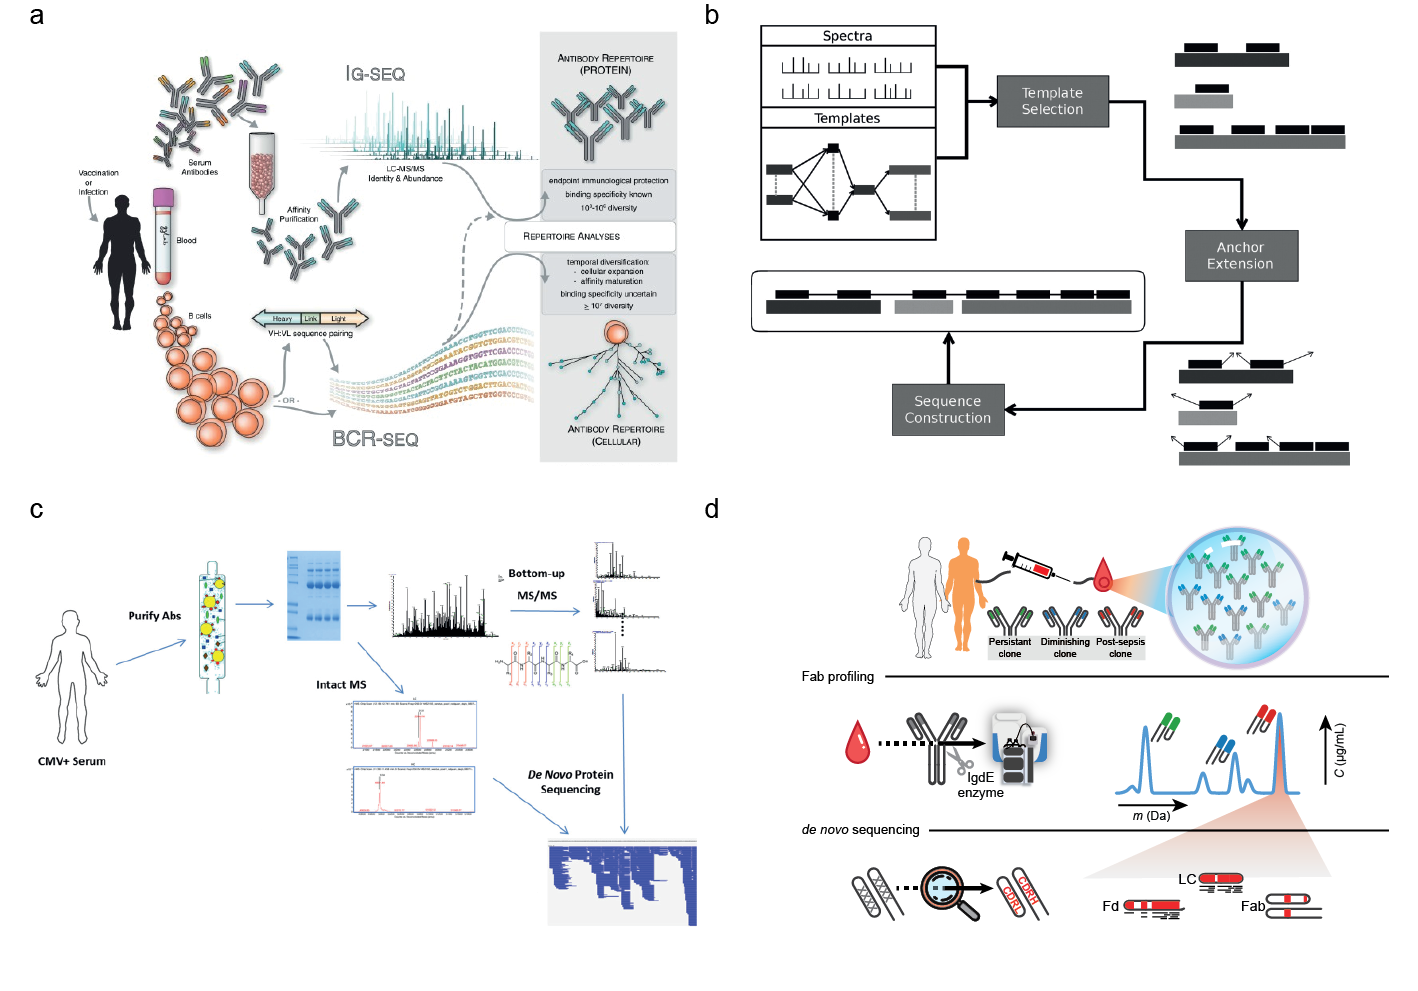
\includegraphics[]{Chapter.1/Figures/f6.png}
  \caption{
    \textbf{Selected recent approaches aiming towards MS-based \emph{de novo} sequencing of serum antibodies.} ~~a) In Ig-seq \cite{lavinder2015next-generation} a personalized database generated by BCR sequences is used to identify specific clones, using tryptic peptides covering the CDR3 region. Figure adapted from Lavinder et al. \cite{lavinder2015next-generation} ~~b) Template proteogenomics \cite{castellana2010template} use genomic data to generate template sequences. The specific construction of the templates can be defined by the user from either whole genome sequencing or BCR sequencing data. Figure adapted from Castellana et al. \cite{castellana2010template} ~~c) PolyExtend \cite{guthals2017de} helped to analyse a polyclonal mixture of antigen-specific purified antibodies measured by BU MS and intact mass measurements. Using a user-assisted algorithm, these data from different MS modalities were combined to sequence the most abundant clones. Figure adapted from Guthals et al. \cite{guthals2017de} ~~d) Fab profiling \cite{bondt2021human} measures and quantifies intact masses of Fabs to provide a view of the IgG1 clonal repertoire, enabling to quantify and monitor individual clones. Abundant serum clones are identified by using BU and MD MS data iteratively to generate full IgG \emph{de novo} sequences. Figure adapted from Bondt et al. \cite{bondt2021human}
  }
  \label{fig:fig1.6}
\end{figure*}


\subsubsection{Alternative proteogenomics approaches}
Extending beyond the Ig-seq strategy, proteogenomics approaches as taken by Castellana et al. \cite{castellana2010template} incorporate personalized genomics data into the antibody sequencing workflow to identify complete antibody sequences. In their software package GenoMS \cite{castellana2010template} they accept both proteomic and genomic databases as input, which are used to reconstruct antibody (sub)sequences from BU MS data. The database is used to find a homologous template sequence, whereby missing, mutated, and spliced genes are considered. The software also allows for a high degree of flexibility through user-defined constraints. In addition, users can define how the template database is used, excluding certain genes, or using multiple gene segments (V, D, J, or C) to make up a single sequence (\textbf{\autoref{fig:fig1.6}b}). As often occurs with hybrid approaches, the power of this proteogenomics strategy comes at a cost. While broadly applicable and very powerful, the required expertise increases because of the use and combination of multiple omics techniques. However, when successfully applied, this workflow produces exciting results, as recently shown in the analyses of antibodies from immunized rabbits \cite{bonissone2020serum} and the characterization of neutralizing antibodies against the Ebola virus antigen \cite{gilchuk2021proteo-genomic} with notable improvements in integration and visualization of the data. Unfortunately, not all these tools are currently publicly available, although several underlying protocols are open source \cite{cha2017antibody, safonova2015igrepertoireconstructor:, bonissone2016immunoglobulin}.

\subsection{Protein-centric sequencing of endogenous antibodies}
Some attempts have emerged aiming at novel antibody discovery by MS-based sequencing alone, directly from serum samples or other liquid biopsies, circumventing the need for genomics/transcriptomics data (multi-omics approaches). Above we reviewed several techniques for sequencing purified antibodies. As we pointed out, these methods are geared towards highly purified mAb samples and are therefore not directly applicable for polyclonal antibody mixtures. However, advancements in sample preparation, instrumentation, and bioinformatics make it possible to obtain partial and sometimes complete \emph{de novo} sequences of endogenous antibody clones by combining different mass spectrometric techniques, as discussed further below.

\subsubsection{Antigen-specific capture}
For many pathologies, it is common to screen patient’s serum for antibodies that exhibit activity against the antigens originating from the pathogen, for example, by enzyme-linked immunosorbent assay (ELISA). Using pathogen-based antigens, it is also possible to capture specific antibody clones from serum that exhibit high affinity against the antigen. This typically reduces the complexity of the antibody mixture substantially. Nevertheless, it is still nearly impossible to reduce the complexity down to a single clone, as often, multiple antibodies with varying affinities for any given antigen co-occur. An example of a capturing method whereby additional intact mass data was used to derive \emph{de novo} sequences was described by Guthals et al. \cite{guthals2017de}. Following affinity purification of antibodies from the serum of a cytomegalovirus-exposed individual, using the glycoprotein B antigen, both intact mass and BU MS measurements were performed. Their semi-automated software PolyExtend seeks to use the intact mass measurements to retrieve the average mass of the most abundant species in an antibody mixture, which in turn is used as a mass constraint for a sequence derived using the BU MS data (\textbf{\autoref{fig:fig1.6}c}). PolyExtend builds further upon the meta-SPS algorithm \cite{guthals2012shotgun}, which was initially designed to extend subsequences by assembling multiple sequence predictions into longer subsequences. However, diverging extensions for the same subsequence are treated as sequencing errors with one extension selected for the output. In the case of antibodies, such divergences may indicate the presence of two similar clones. To account for this, the software displays the possible extensions as a ranked list, and the user can then select the extension. This approach aims at expanding the \emph{de novo} sequencing capabilities of the previously established meta-SPS algorithm to deal with simultaneous presence of multiple clones, and Guthals et al. \cite{guthals2017de} demonstrated a clear proof of concept.

\subsubsection{Antibody profiling and sequencing in polyclonal mixtures}
While it is still not possible to \emph{de novo} sequence entire serum antibody repertoires, recent advances in LC-MS of intact proteins enabled detecting and resolving single clones from complex antibody mixtures.
For instance, developments have been made that specifically profile intact light chains from serum, even providing partial sequence information by using MD MS. Impressively these studies successfully demonstrate the analysis in serum without requiring antigen-specific capture, although they used either a spiked-in mAb as a model or worked with disease models that cause monoclonal Ig overexpression in serum (mono-gammopathy) such as multiple myeloma. Nonetheless, these studies demonstrated that detection and characterization of individual endogenous light chains is possible \cite{he2017analysis, he2019classification, mills2015detecting, sharpley2019novel, dupré2021de}. Taking this one step further, Wang et al. \cite{wang2019top-down} developed a method to detect individual Fab fragments in serum. They were able to identify tens of heavy and light chains of serum autoantibodies. Although attempts were made to \emph{de novo} sequence these antibodies at the intact protein level, the obtained results were limited to a few sequence tags. In light of the SARS-CoV-2 pandemic, Melani et al. \cite{melani2022next-generation} focused their profiling efforts on the vaccine-targeted spike protein receptor-binding domain. The approach is named Ig-MS and features two novel metrics for capturing the intensity and complexity of the antibody response. In short, the method uses affinity purification to capture antigen-specific clones. A mAb-containing standard is spiked in for quantitation, and the sample is disulphide-reduced. After reduction, individual ion MS \cite{kafader2020multiplexed} is used to measure a mass fingerprint of the sample. The ratio between the intensity of clonal peaks and the standard is used to estimate the response (“Ion Titer”), and the complexity of the response (“Degree of Clonality’) is assessed by the ratio of the most intense light chain peak to that of the summed intensity of all light chain peaks. Finally, these metrics are correlated to the ELISA-based antibody titer and neutralization efficiency, to verify their accuracy.
In a recent study, Bondt et al. \cite{bondt2021human} used an approach to generate Fab fragments exclusively from the entire IgG1 repertoire. They were able to longitudinally profile IgG1 Fabs from the serum of both healthy and sepsis-inflicted donors without the need for any enrichment of specific clones. They observed a range of 50-500 distinct detectable IgG1 Fab clones per donor and showed that most clones persist over multiple months of sampling. Contrary to widely held belief, they showed that the IgG1 repertoire is in abundance dominated by just a few hundred clones and that each donor exhibits a unique repertoire of clones. They also managed to directly \emph{de novo} sequence a single highly abundant clone in one of the donors without the aid of antigen-specific capture. The \emph{de novo} sequencing was achieved by a combination of protein-centric sequencing using ETD, and a BU MS approach using multiple proteases for digestion. First, closely matching light and heavy chain germline templates were selected from the IMGT database. Subsequently, the data was used to refine these templates iteratively, yielding the final mature sequence. This provided proof of concept that \emph{de novo} sequencing of clones directly from serum is feasible, although still arduous and limited to specific cases (\textbf{\autoref{fig:fig1.6}d}). Notably, the determined sequences contained more mutations (compared to germline sequences) than expected from the reported rates from BCR sequencing studies \cite{kitaura2017different}, which is indicative of potential discrepancies between protein-level and gene-level sequencing. This first attempt focused exclusively on IgG1, by using an IgG1-specific protease to generate the Fab fragments. In another work, Bondt et al. \cite{bondt2021direct} extended their method to IgA1 by using a protease specific to the O-glycans present in IgA1 hinge region to generate Fab fragments, albeit now exclusively from IgA1. Overall, they showed that – similar to serum IgG1 – just a handful of clones dominates the secretory IgA1 profile of human milk.
Using a somewhat comparable approach, Dupré et al. \cite{dupré2021de} analysed isolated light chains from the urine of a patient affected by multiple myeloma. They assembled \emph{de novo} data from peptides into a full-length sequence, using the intact mass data as a scaffold. Subsequently, they used TD MS to validate their findings and further characterize the proteoforms of the light chains, including PTMs. The BU MS data further supported the resulting proteoforms, showing a similar added benefit from iteratively combining BU and TD MS data.

\subsection{Additional benefits of studying antibodies at the protein level}
The capabilities of MS allow for antibody characterization beyond the primary amino acid sequence. Antibodies are known to harbour multiple important PTMs: Fab- and Fc-glycosylation \cite{haan2020monitoring}, deamidation \cite{yan2018structure}, and C-terminal truncation \cite{beyer2018microheterogeneity}, to name a few. Moreover, although the disulphide bonds in IgG1 are thoroughly described, other subclasses, notably IgG2, appear to occur as structural isomers induced by different disulphide-bridge patterns. These PTMs and disulphide bridges become even more pronounced in IgA and IgM, which can form higher-order structures connected by the joining-chain in serum and other bodily fluids. All these features influence the antibody’s efficacy and stability. Such information cannot easily be obtained at the nucleotide level, requiring protein-level analysis.
\clearpage

\section{Thesis overview}
Throughout this thesis, I detail my efforts to develop computational workflows and tools that facilitate the analysis of complex LC-MS proteomics data. There is a strong focus on the analysis of antibody repertoires, apart from Chapter 2 which focuses on analyzing cross-linking MS data. The work described in this chapter shaped what became the guiding principle of my academic efforts; that \emph{standardized computational tools are of vital importance for reproducible research}. As such, I consider it the spiritual predecessor to the subsequent chapters and an important example of the central theme.
\bigskip\\
\textbf{Chapter 2} describes how we developed CrossID, a tool to analyze large and complex cross-linking proteomic datasets. CrossID was developed to facilitate explorative analysis of large amounts of crosslinking data. We show that integration of data from multiple sources can provide valuable insights, as the integrated data from protein databases enables gene ontology enrichment analysis and grouping based on function. Furthermore, we showcase how mapping of crosslinked residues onto 3D-structural models for proteins can help refine these models or help to generate models for protein complexes.
\bigskip\\
In \textbf{Chapter 3}, the LC-MS based antibody repertoire profiling approach which enabled the research in \textbf{Chapter 4} and \textbf{5} is introduced. In this initial application of the technique on a cohort of sepsis patients we found the serological IgG1 repertoires to be unique to each individual, stable over time, responsive to physiological events and relatively simple, consisting of several hundred clones despite there being an enormous number of theoretically possible clones. Furthermore, this chapter provides proof of concept for \emph{de novo} sequencing of endogenous antibodies by using a multi-tier mass spectrometry approach to sequence the most abundant clone for a donor.
\bigskip\\
\textbf{Chapter 4} describes the analysis of breastmilk SIgA1 profiles of six mothers who had received two identical SARS-CoV-2 vaccinations over 16 timepoints. We use the extensive sampling and repeated vaccination to define clonal populations based on the detection window of these clones relative to the vaccination events. We also discover that the second vaccination induces the emergence of a population of novel clones and show that titer fluctuations as measured by ELISA can be driven by highly divergent clonal populations.
\bigskip\\
In \textbf{Chapter 5}, we build upon the proof of concept for \emph{de novo} sequencing of endogenous antibodies by hybrid top-down and bottom-up mass spectrometry approaches. We present a more standardized workflow for sequencing antibody chains in mixtures. Our approach resolves ambiguity in sequence predictions for the hypervariable complementarity determining regions by mass-filtering candidate sequences based on the gap size between adjacent framework regions, which we determine using middle-down fragmentation data.
\bigskip\\
Finally, \textbf{Chapter 6} contains a summary and a discussion of the advances that enabled the work in this thesis, the impact of the findings for others in the field, the challenges that lay ahead and how they may be overcome, along with an outlook on where I believe the field is heading.
\newpage
\section*{References}
\bibliographystyle{Stylesettings/pnas}
\patchcmd{\thebibliography}
{\clubpenalty 4000\widowpenalty 4000}
{\clubpenalties 1 10000 \widowpenalties 1 10000}
{}{}
\bibliography{chapmerge}
\stopthumb


%%refs (does not alter the tex cause commented, just for retrieval)
%% \cite{georgiou2014promise}

\picturechapter{Cross-ID: Analysis and visualization of complex XL−MS-driven
  protein interaction networks}{Chaptercovers/ch2.pdf} \label{ch-2}
\vspace*{0.25cm}

{\footnotesize Sebastiaan C. de Graaf\textsuperscript{*}, Oleg Klykov\textsuperscript{*}, Henk van den Toorn, and Richard A. Scheltema}

\begin{center}
  \vspace{3cm}
  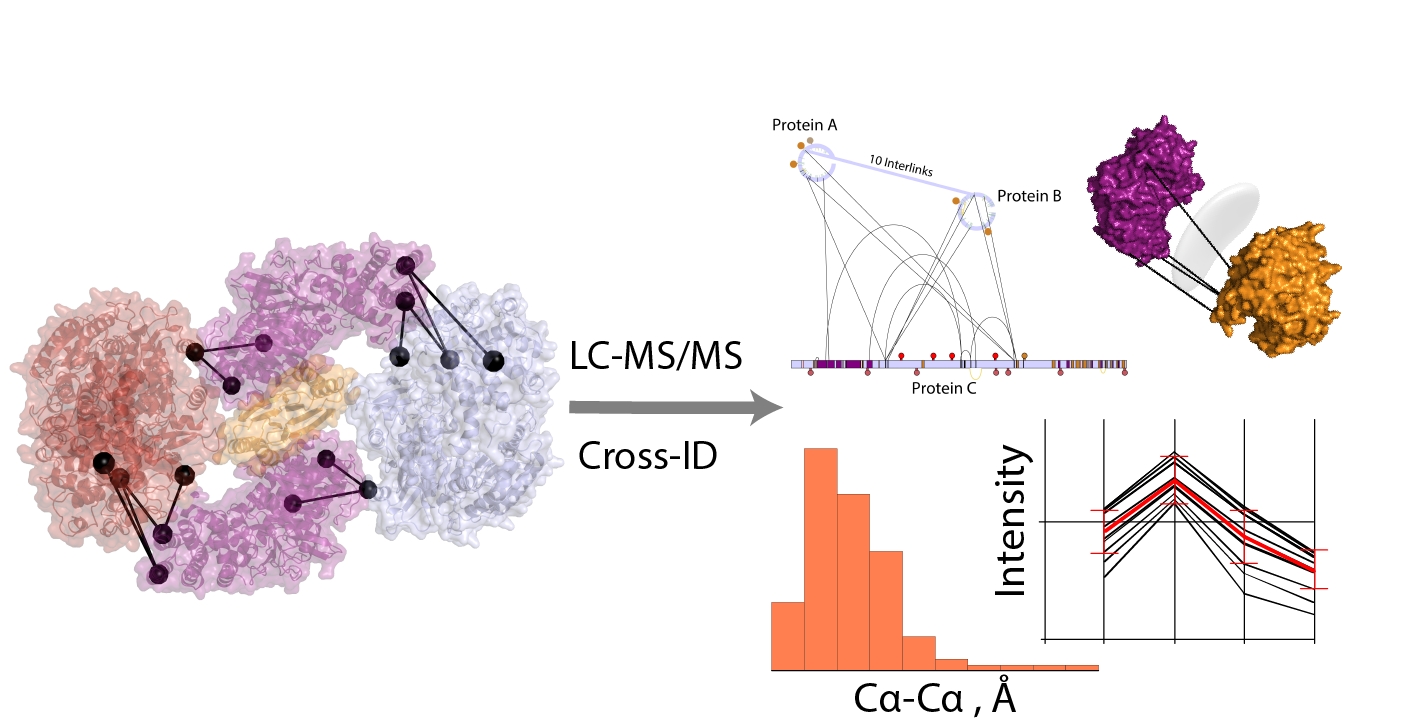
\includegraphics[]{Chapter.2/Figures/ch2.png}
  \vspace{0.25cm}
\end{center}

\begin{flushleft}
  \vspace*{\fill}
  \rule{\textwidth}{1pt}\\[0cm]
  \textbf{This chapter is based on work in the following publication:}\\
  \footnotesize{
    \textbf{Cross-ID: Analysis and Visualization of Complex XL−MS-Driven
      Protein Interaction Networks, \emph{Journal of Proteome Research}} (2019), 18:642-651, doi:10.1021/acs.jproteome.8b00725\\
    %%\footnotesize
    \vspace{0.3cm}
    \textsuperscript{*} These authors contributed equally to this work}
\end{flushleft}

\begin{abstract102}
  Protein interactions enable much more complex behavior than the sum of the individual protein parts would suggest and represents a level of biological complexity requiring full understanding when unravelling cellular processes. Crosslinking mass spectrometry has emerged as an attractive approach to study these interactions and recent advances in mass spectrometry and data analysis software have enabled the identification of thousands of crosslinks from a single experiment. The resulting data complexity is however difficult to understand and requires interactive software tools. Even though solutions are available, these represent an agglomerate of possibilities and each features its own input format often forcing manual conversion. Here we present Cross-ID, a visualization platform that links directly into the output of XlinkX for Proteome Discoverer, but also plays well with other platforms by supporting a user-controllable text-file importer. The platform includes features like grouping, spectral viewer, GO enrichment, PTM-visualization, domain- and secondary structure mapping, dataset comparison, pre-visualization overlap-check and more. Validation of detected crosslinks is available for proteins and complexes with known structure or for protein complexes through the DisVis online platform. Graphs are exportable in PDF format, and datasets can be exported in tab separated text files for evaluation through other software.
\end{abstract102}
\thumbforchapter

\section{Introduction}
\lettrine[lraise=0.1, nindent=0em, slope=-.5em]{P}{rotein}
interactions represent a level of cellular complexity that is essential for almost all biological processes. The protein assemblies they represent are highly dynamic and orchestrate cellular processes by regulating enzymes and forming macromolecular clusters capable of more complex behavior than the sum of their parts would suggest. Crosslinking mass spectrometry (XL-MS) has emerged as an attractive approach to elucidate protein-protein interactions (PPIs) by mass spectrometry. It uses small reagents with two reactive moieties capable of forging a covalent bond between two amino acids in close proximity. Upon application to proteins and protein-protein complexes followed by their proteolytic digestion, four distinct peptide products are formed: non-modified, mono-linked, loop-linked, and crosslinked peptides \cite{schilling2003ms}. The first three product groups consist of single peptides in various forms that yield limited or no structural information. The fourth group consists of two peptides captured by the crosslinking reagent; this yields valuable distance information for the elucidation of protein tertiary structure (the two peptides originate from the same protein) or protein quaternary structure (the two peptides originate from different proteins). Identification of both peptides by mass spectrometry allows for localization of the crosslink within the proteins of interest. Although several well established methods like affinity purification mass spectrometry (AP-MS) \cite{fagerlund2017spacer, benda2014structural, joachimiak2014structural, herzog2012structural, chen2010architecture, armony2016cross-linking} are available for studying PPIs at high speeds \cite{hosp2015double-barrel}, most of these are limited to stable interactions and/or provide little to no structural information. XL-MS on the other hand has the potential to capture weak and transient interactions complete with structural information. With recent advances in mass spectrometry, crosslinker chemistry, pre-fractionation techniques and data analysis software, XL-MS can now routinely detect thousands of crosslinked peptides from a single experiment \cite{kao2011development, liu2015proteome-wide, liu2017optimized, schweppe2017mitochondrial}. Even in the case of single proteins, XL-MS can yield hundreds of detected distance restraints \cite{belsom2017complementary}.
\begin{figure*}[!htb]
  \center
  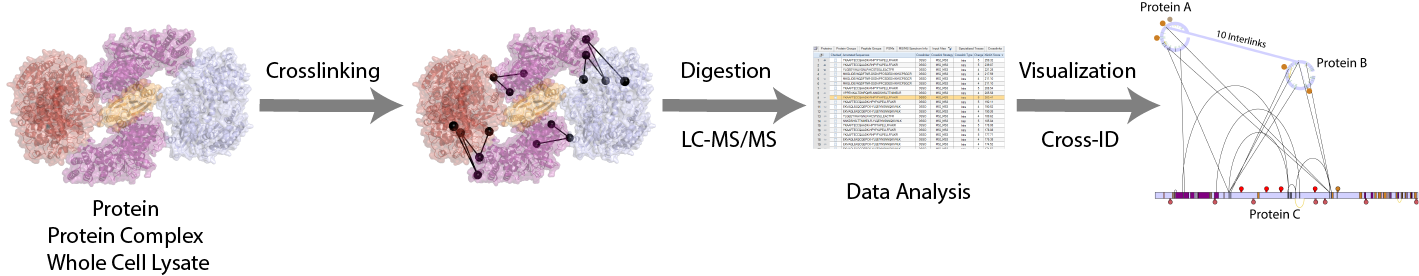
\includegraphics[]{Chapter.2/Figures/f1.png}
  \captionsetup{singlelinecheck = false, format= hang}
  \caption{\textbf{Visualization with Cross-ID.}}
  \label{fig:fig2.1}
\end{figure*}

\begin{figure*}[!htb]
  \center
  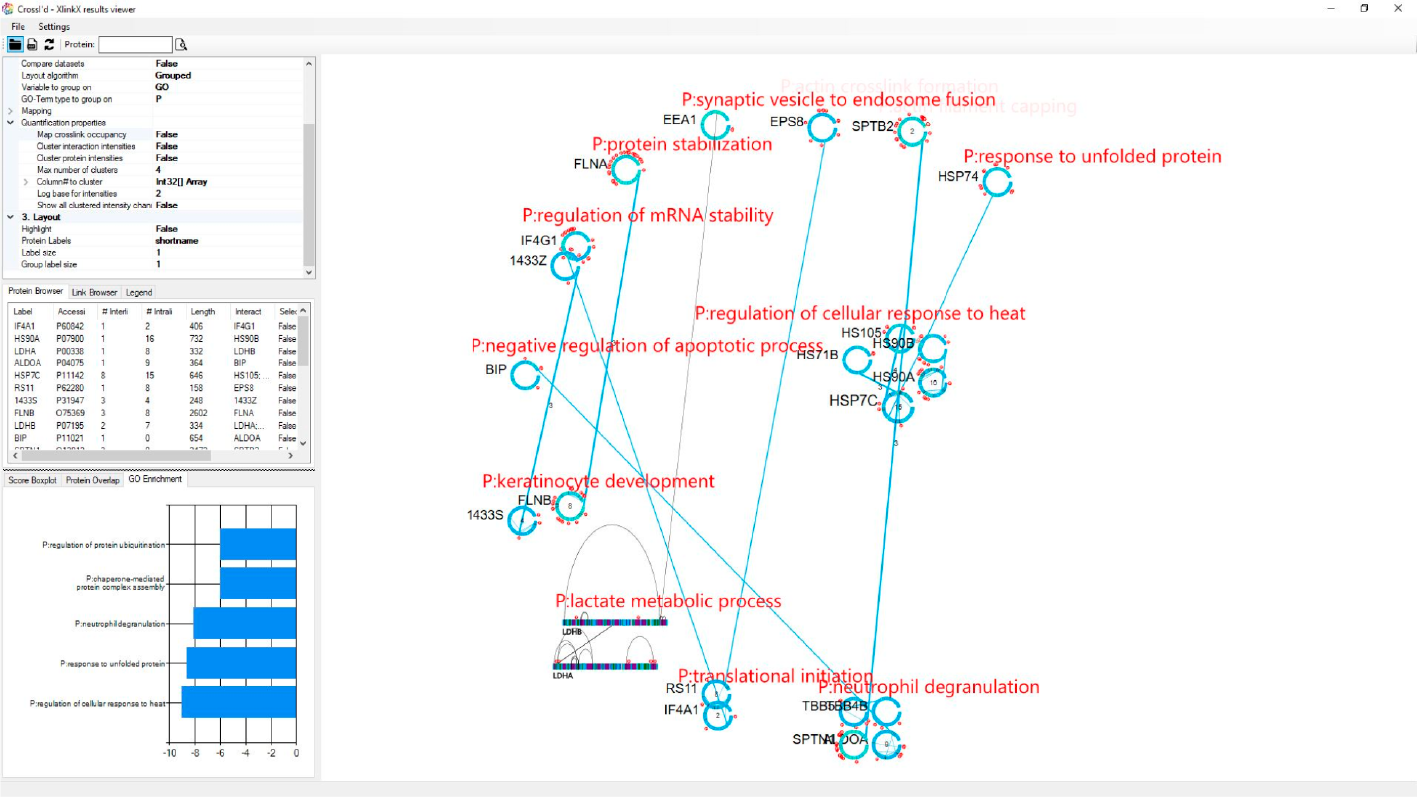
\includegraphics[]{Chapter.2/Figures/f2.png}
  \captionsetup{singlelinecheck = false, format= hang}
  \caption{\textbf{Screenshot of Cross-ID.}}
  \label{fig:fig2.2}
\end{figure*}

An attractive means to obtain a bird’s-eye view of the crosslinking results are network graphs \cite{shannon2003cytoscape:, cline2007integration, bastian2009gephi:}. This type of visualization however also becomes cumbersome to read for increasing sizes of the depicted datasets, where the large number of nodes and edges can easily obfuscate the view \cite{agapito2013visualization}. Additionally, when no connection between the visualized elements and the initial input datasets exists it remains very difficult for the user to browse the data and check for validity. To circumvent these obstacles advanced software allowing the network to be visualized, organized and filtered in real-time is needed. Several software platforms partly supporting such features exist \cite{courcelles2017clmsvault:, heymann2008msx-, kahraman2011xwalk:, kosinski2015xlink, lima2015sim-xl:, riffle2016proxl, schweppe2015xlmap:, schweppe2016xlinkdb, solis-mezarino2017complexview:}, with varying degrees of specificity towards XL-MS. The most widely used examples consist of xiNet \cite{combe2015xinet:} and xVis \cite{grimm2015xvis:}. Each of these tools has a unique set of features and each offers a different subset of visualization options, which tailors them for particular applications (e.g. Xwalk \cite{kahraman2011xwalk:} calculates solvent accessible surface distances or XlinkAnalyzer \cite{kosinski2015xlink} fits distance restraints to a given 3D model). However, when it comes to visualization of large scale crosslinking datasets like whole cell lysates, a combination of software solutions is often required. Proteome-wide interactomes can for example be visualized with biological network builders such as Cytoscape \cite{shannon2003cytoscape:, cline2007integration}, but there are no tools specifically tailored towards in-depth analysis of large proteome-wide XL-MS datasets. Added to this, relatively few tools support generic input formats from multiple software platforms (prominent example which do include this are xiNET \cite{combe2015xinet:} and ProXL \cite{riffle2016proxl} ); however, most are tightly linked to a specific search engine or define their own data format requiring cumbersome file format changes to compare results between different datasets.
Here we present Cross-ID, a standalone solution for visualization of XL-MS data as network graphs. It provides a direct connection to the output of XlinkX for Proteome Discoverer 2.3 but also supports an importer for comma-separated text output generated by any XL-MS search engine. Additional to crosslinking data, Cross-ID can display any data containing connection or distance restrains (e.g. small-angle X-ray scattering or SAXS data \cite{morimoto2013small-angle} ) as long as it is available in a tabular form. The importer uses natural language processing to predict the use of each column-header in the output file and allows the user to make adjustments where required. The generated graphs are highly interactive and can be explored by filtering, expanding, repositioning, highlighting, mapping or altering the graph directly. Ultimately, this will enable the user to draw meaningful conclusions from the graphs edited inside Cross-ID and without the need for editing the input dataset each time before uploading. It is also possible to group proteins based on detected interlinks or according to other parameters (e.g. their GO enrichment coefficient), significantly simplifying the data analysis. A number of site-specific findings from the Uniprot database \cite{bateman2017uniprot:} (among others glycosylation, disulfide bridges and phosphorylation sites) can be mapped onto all protein representations, as well as residues of interest. In addition, it is also possible to depict specific modifications detected by the search engine and quantitation by various methods. Cross-ID also supports validation of crosslinks for a single protein or protein complex using available structures in protein data bank (PDB) format. Alternatively, Cross-ID provides a direct link to DisVis for validating potentially interacting partners based on the detected crosslinks \cite{zundert2016disvis, zundert2015disvis:}. As a showcase study we provide a whole cell lysate dataset with 2754 crosslink spectra matches (CSMs), obtained from PC9 cells. To showcase the quantitation functionalities we used Tandem Mass Tag (TMT) quantitation to quantitate protein kinase A (PKA), activated upon addition of cAMP as a model system.


\section{Materials and Methods}

\subsection{DSSO Protein-Protein Crosslinking}
Crosslinked cell lysates have been prepared as previously described \cite{klykov2018efficient}. Briefly, PC9 (Sigma-Aldrich, Steinheim, DE) cells were collected and washed 3x with PBS (Lonza, Basel, SUI). After centrifugation, the cell pellet was resuspended in crosslinking buffer consisting of 50 mM HEPES, 150 mM NaCl and 1.5 mM MgCl\textsubscript{2} (all from Sigma-Aldrich, Steinheim, DE). Protease inhibitors (Roche, Basel, SUI) and 0.5 mM DTT (Sigma-Aldrich, Steinheim, DE) were added right before use. After the cells were lysed with a Bioruptor (Diagenode SA, Seraing, BE), freshly dissolved disuccinimidyl sulfoxide or DSSO in DMSO (Sigma-Aldrich, Steinheim, DE) was added to a final concentration of 2 mM. The crosslinking reaction was quenched after 30 minutes with Tris-HCl at a final concentration of 20 mM. The crosslinked proteins were denatured and reduced and alkylated in a mixture of 8 M Urea, TCEP and CAA. Proteolytic digestion was performed in 2 steps: for 30 min with LysC (Wako, Tokyo, JPN) at room temperature and overnight with Trypsin (Promega, Madison, WI, USA) at 37 ⁰C. Digested peptides were desalted with a Sep-Pak cartridge and dried prior to fractionation.


\subsection{Fractionation of Crosslinked Peptides}
Strong Cation Exchange (SCX) chromatography was performed on an Agilent 1200 HPLC system (Agilent Technologies, Waldbronn, DE). The setup was previously described \cite{hennrich2011improving}, but shortly consists of an Opti-Lynx trap column connected to a PolyLC SCX-separation column (PolyLC Inc., Columbia, MD, USA). Peptide mixtures were reconstituted in 5\% DMSO/10\% formic acid/85\% water (v/v/v) and separated over a gradient of 120 minutes, resulting in 50 collected factions. A total of 15 crosslinks-rich fractions were chosen for analysis and prior to further analysis dried and stored at -80 ⁰C.


\subsection{LC-MS/MS Analysis}
Peptide mixtures were reconstituted in 5\% DMSO/10\% formic acid/85\% water (v/v/v) and analyzed on an Orbitrap Fusion Lumos (Thermo Fisher Scientific, San Jose, CA, USA) coupled online to an Agilent 1290 UPLC (Agilent Technologies, Waldbronn, DE). Peptides were trapped on a double-frit C\textsubscript{18} pre-column (Reprosil C\textsubscript{18}, Dr. Maisch, 100 µm x 2 cm, 3 µm; packed in-house) for 5 min with buffer A (0.1\% formic acid) and separated on a single-frit analytical column (Poroshell 120 EC C18, Agilent Technologies, 50 µm x 50 cm, 2.7 µm) over 155 minutes with a linear gradient from 10\% to 40\% B (B: 0.1\% formic acid, 80\% acetonitrile). Optimized MS settings were described previously \cite{liu2017optimized, klykov2018efficient}. Acquired data were analyzed with the Proteome Discoverer software suite 2.3 (Thermo Fisher Scientific, San Jose, CA, USA) with incorporated XlinkX nodes. Spectra were matched against the Homo sapiens database from SwissProt (version 2018\_06, 20,349 sequences, downloaded from Uniprot). The protease was set to “Trypsin” and the maximum number of missed cleavages was defined as 2. Carbamidomethylation of cysteines was set as fixed modification and oxidation of methionine and protein N-terminal acetylation as variable modifications. For the linear peptide search, precursor mass tolerance was defined as 20 ppm and fragment mass tolerance as 0.5 Da for ion trap readout or 20 ppm for the Orbitrap readout. For the crosslinked peptides search, the minimum peptide length was set to 5 and minimum peptide mass to 300, while the maximum peptide mass was set to 7000. The precursor mass tolerance was set to 10 ppm, FTMS fragment mass tolerance at 20 ppm and ITMS fragment mass at 0.5 Da. FDR threshold was set to 0.01 (1\%) and FDR strategy as “Percolator”.


\subsection{TMT Experiments}
TMT labels were purchased from Thermo Fisher Scientific (San Jose, CA, USA) and the labelling protocol performed according to supplier instructions after desalting of the crosslinked peptides. 10 channels were used to label 10 samples of model system PKA (Sigma-Aldrich, Steinheim, DE) solubilized at a concentration of 5.74 µM with added cAMP (Sigma-Aldrich, Steinheim, DE) ligand to the final concentration of 0-8 µM and 10 µM respectively. Digestion, fractionation and LC-MS/MS analysis were performed according to the procedure described above, except for alterations to the LC gradient consisting of increasing the starting point from 5\% to 36\% of buffer B. For this data, the Orbitrap Fusion (Thermo Fisher Scientific, San Jose, CA, USA) with tune page version 3.1.2412.14 was used for data acquisition with the standard template for TMT labeled crosslinking samples. For data analysis, the TMT-specific nodes were added to the standard crosslinking data acquisition protocol \cite{klykov2018efficient} after “Precursor Ion Exclusion” node namely: “Isobaric Tag Loss” was set to TMT, “Precursor Selection Range” with Mass Range 400-1200 \emph{m/z} followed by 10 SPS scans with HCD at 65\% NCE and resolution of 50000 in Orbitrap. Recorded data were searched against PKA protein complex proteins with 200 Human proteins as decoys taken from the reviewed Swiss-Prot database. In addition to the standard XlinkX processing workflow, “Reporter Ions Quantifier” node was added with “Integration Tolerance” set to 0.03 Da and “Centroid With Smallest Delta Mass” as “Integration Method”. For the consensus workflow, “Reporter Ions Quantified” node was included with standard settings.
\begin{figure*}[!htb]
  \center
  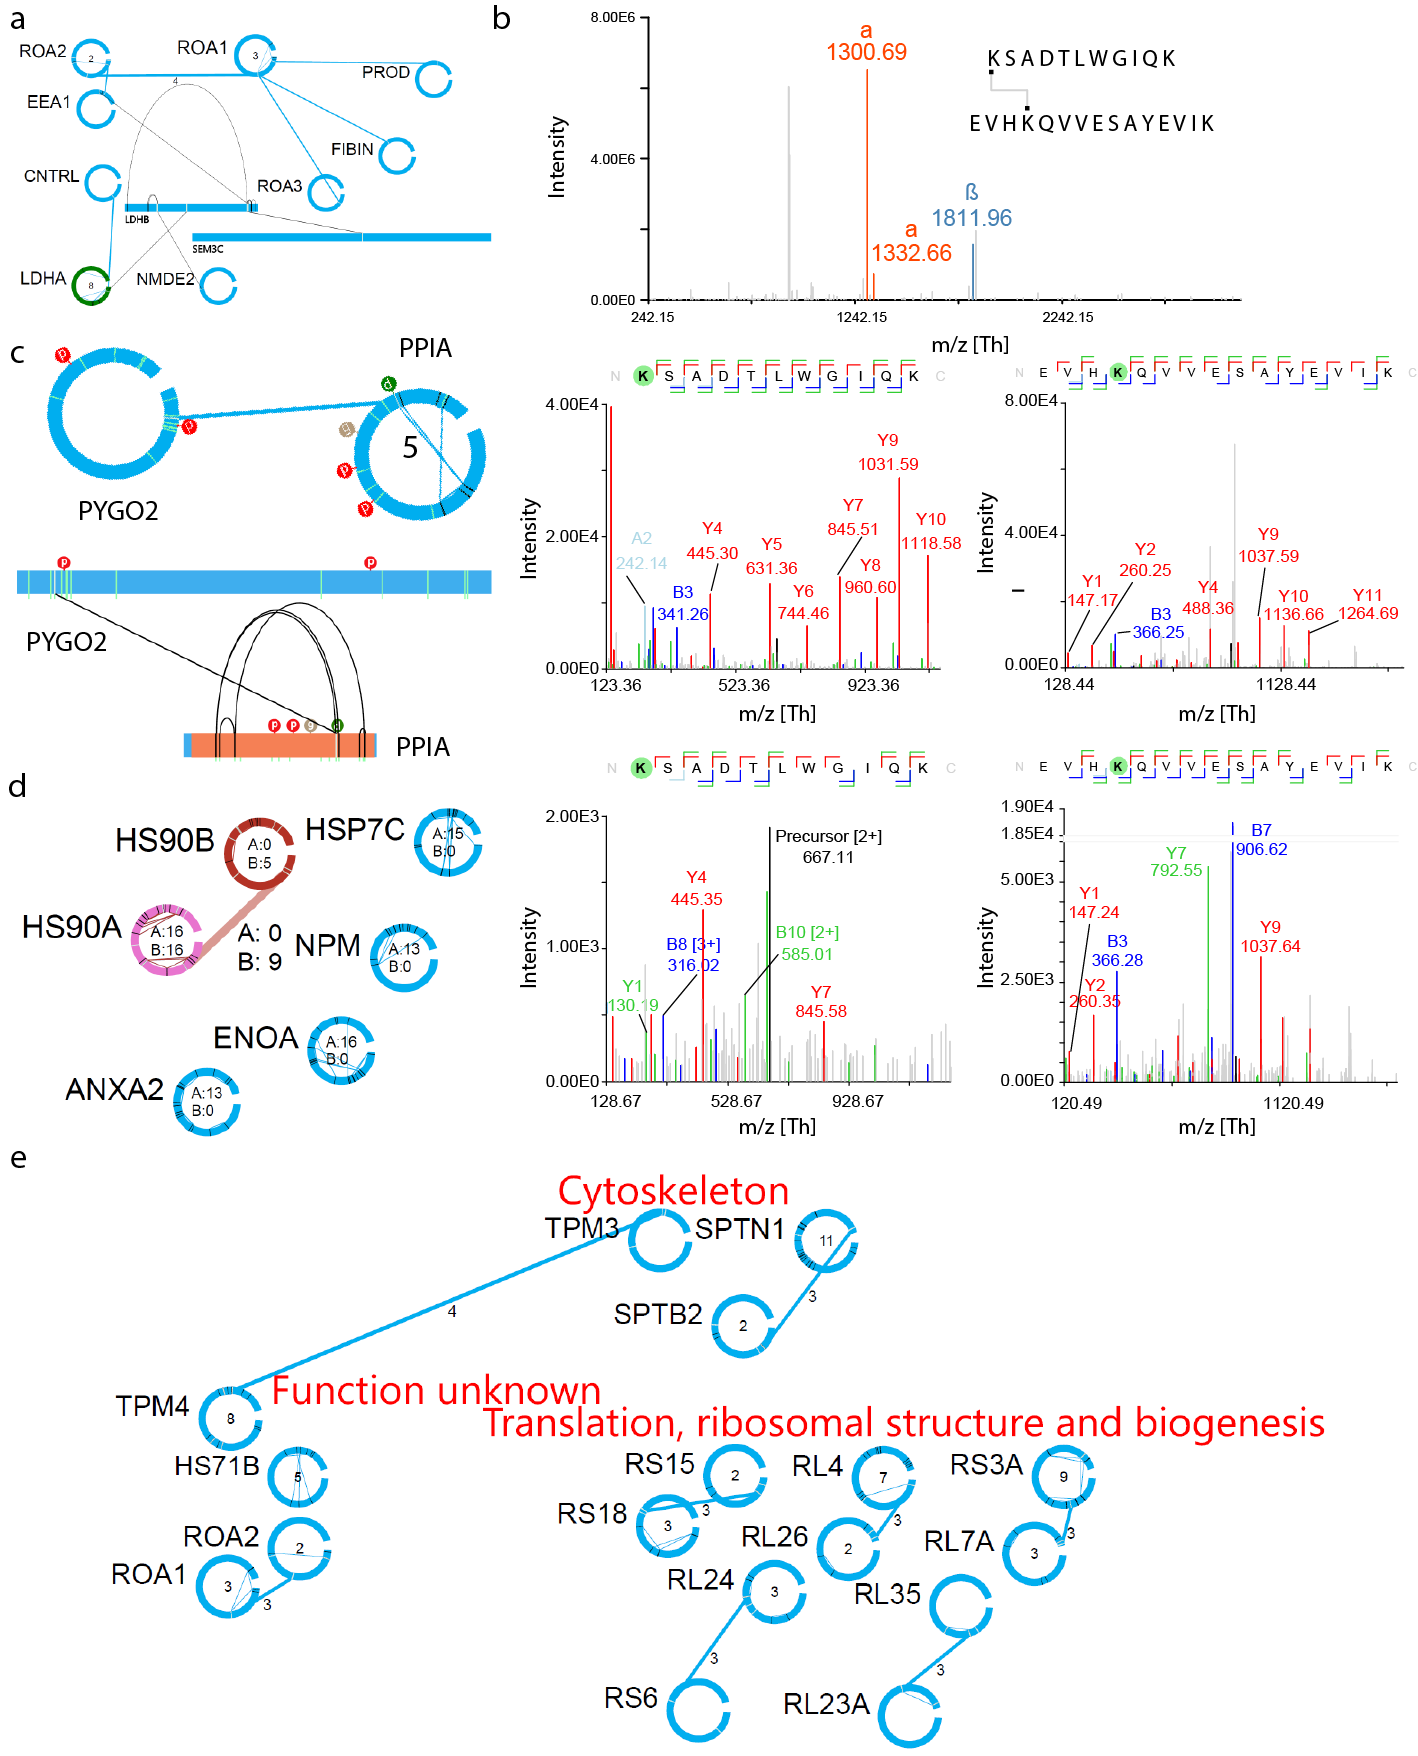
\includegraphics[]{Chapter.2/Figures/f3.png}
  \caption{
    \textbf{Visualization with Cross-ID on a PC9 whole proteome data set.} ~~a) Snapshot of the generated protein interaction network. ~~b) Spectral viewer for selected top-scored cross-links. ~~c) Comparison of bar and circle views for filtered proteins with depicted phosphorylation, glycosylation, and DSSO monolinks together with the known protein domain. ~~d) Comparison of cross-links filtered by XlinkX score at 50 with 13 intralinks and 7 interlinks. ~~e) Clustering according to the EggNOGG database for filtered proteins.
  }
  \label{fig:fig2.3}
\end{figure*}


\subsection{Software and Data Availability}
Cross-ID was developed in Microsoft Visual Studio 2017 as a C\# WinForms application using Windows Presentation Foundation elements. The GraphX .NET library was used as the foundation for the network visualizations. For running the tool, minimally .NET version 4.7 needs to be installed. The software can be downloaded from https://www.hecklab.com/software/xlinkx/ together with an instruction video. The raw data, all the associated output and databases used in this study have been deposited to the Proteome-Xchange Consortium \cite{vizcaíno2014proteomexchange} via the PRIDE partner repository with the identifier PXD008418 (already published and openly accessible) for the whole-proteome dataset and PXD011077 (user: reviewer59676@ebi.ac.uk; password: 7H5TMR0l) for the TMT dataset.
\begin{figure*}[!htb]
  \center
  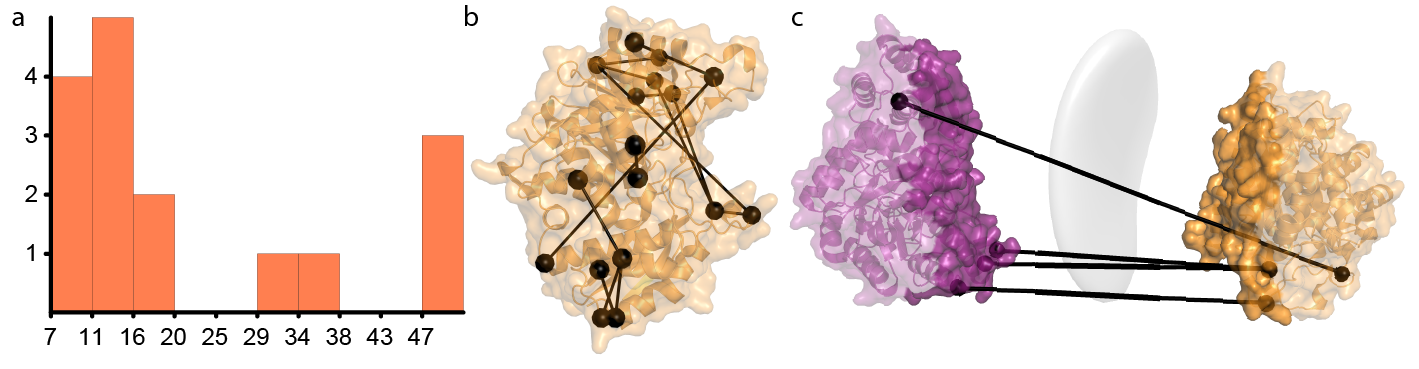
\includegraphics[]{Chapter.2/Figures/f4.png}
  \caption{
    \textbf{Validation of cross-links detected for alpha-enolase.} ~~a) Distance distribution of mapped cross-links on alpha-enolase. ~~b) Detected crosslinks on crystal structure. ~~c) Interaction interface generated by DisVis based on indicated restraints (grey surface) in comparison to the existing dimeric interface (dark purple and dark orange).
  }
  \label{fig:fig2.4}
\end{figure*}
\begin{table*}[!htb]
  \center
  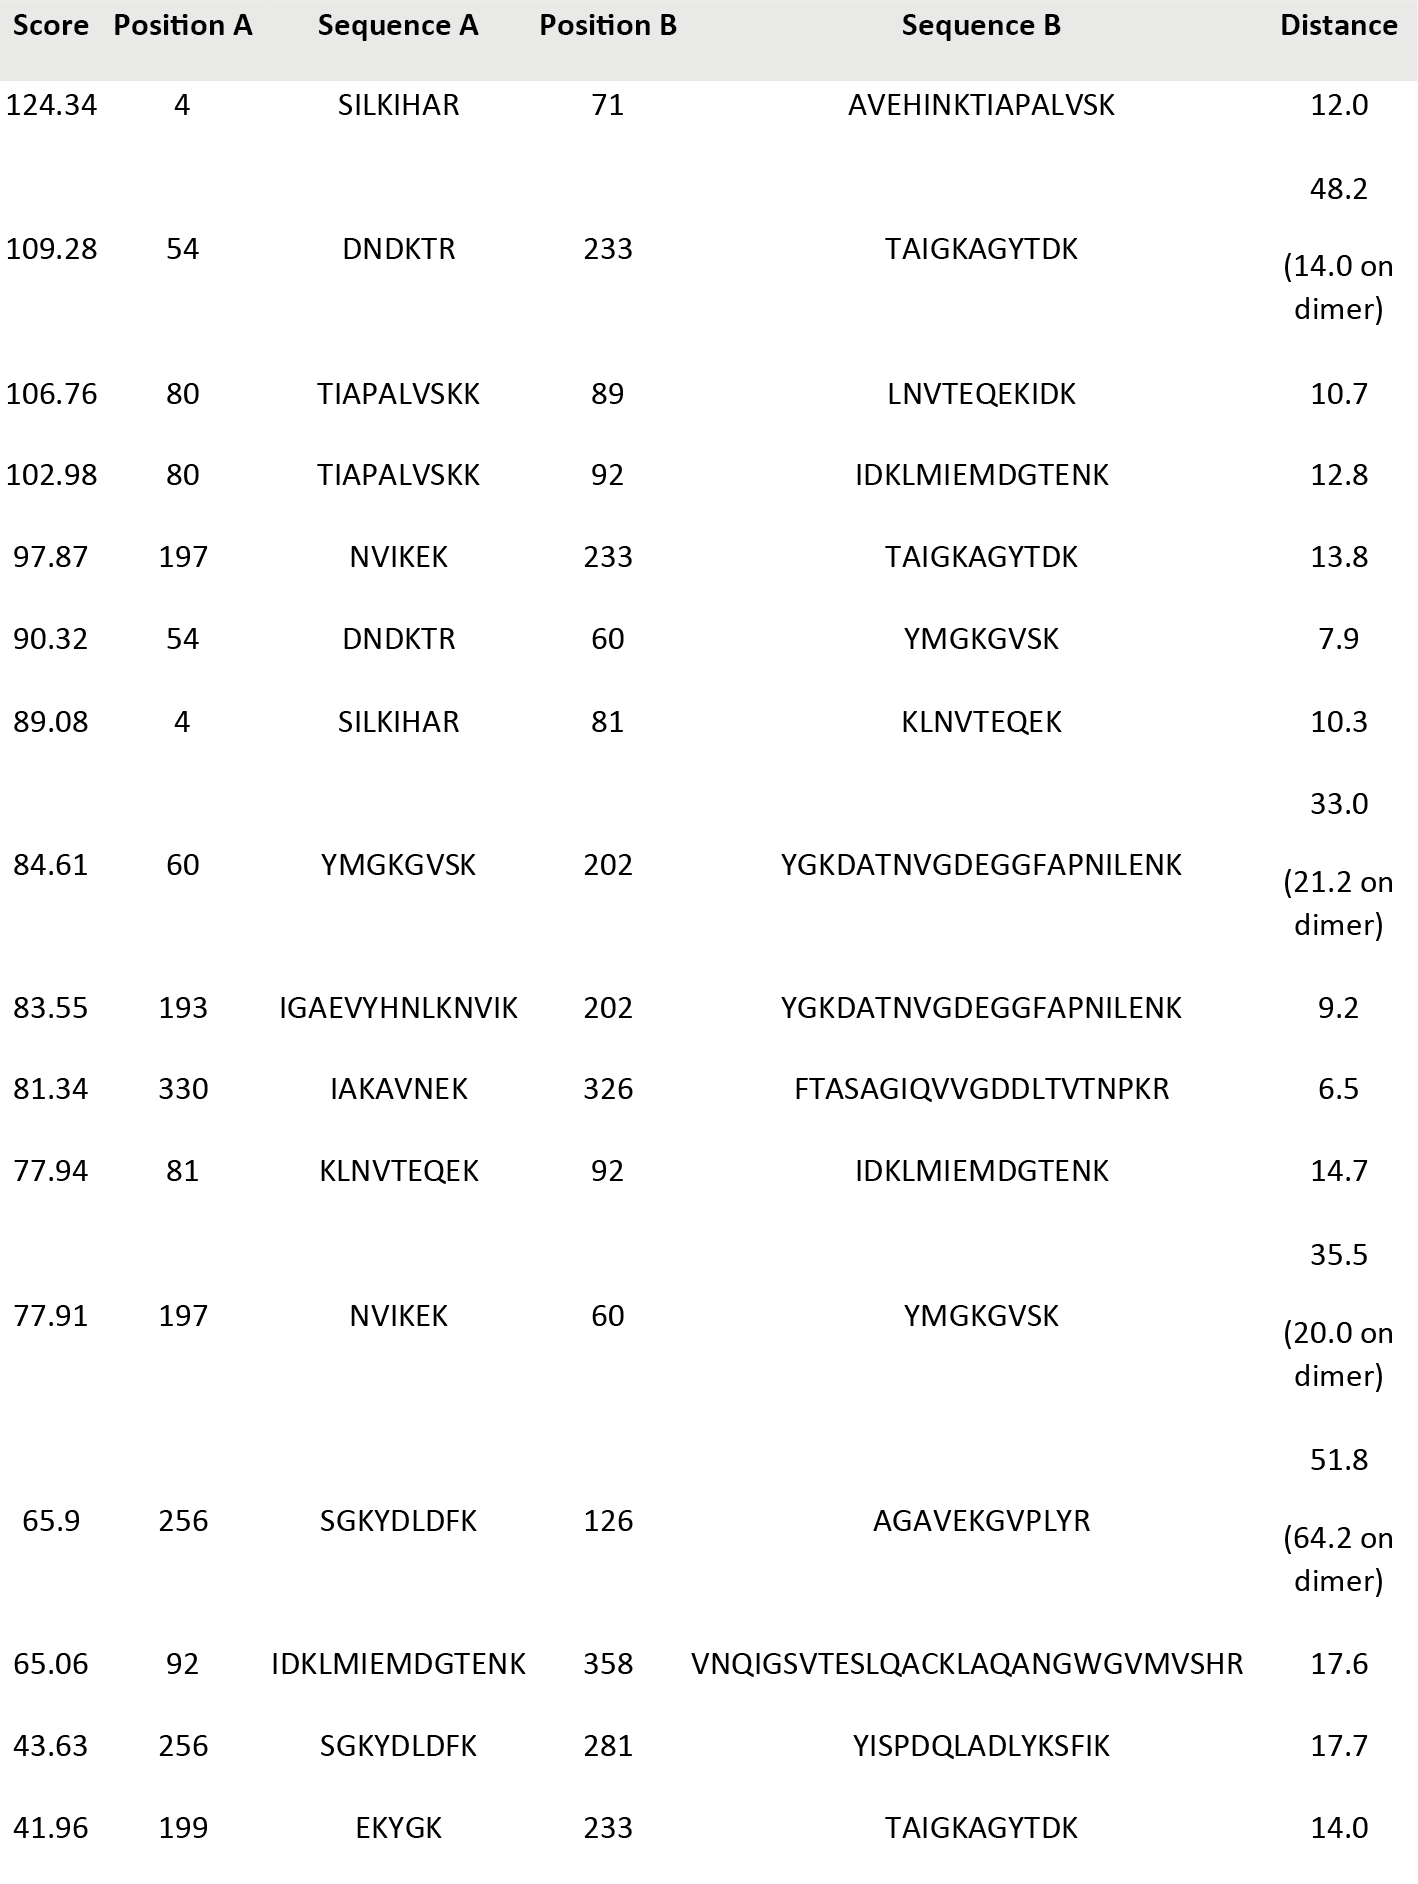
\includegraphics[]{Chapter.2/Figures/t1.png}
  \captionsetup{singlelinecheck = false, format= hang}
  \caption{
    \textbf{List of Crosslinks Detected for Alpha-Enolase.}\\
  }
  \label{tab:tab2.1}
\end{table*}

\section{Results and Discussion}

\subsection{Data Import}
Cross-ID provides a direct link to the output generated by the XlinkX nodes integrated in the Proteome Discoverer data analysis environment \cite{klykov2018efficient}. The files with extension ‘.pdResult’ contain all information required to build the visualization of the network, including the spectra and protein information, together with the tables generated by XlinkX. By loading this directly, correctness and access to all required information is ensured. To work with output from other search engines, Cross-ID provides a convenient import interface for tab- or comma-delimited text files, with column names on the first line. Since column names are not fixed between different search engines, or even in some cases between different versions of the same search engine, Cross-ID assists in manually selecting the correct columns. It provides a prediction of the purpose of each column by calculating a Levenshtein distance \cite{levenstein1966binary} to pre-defined column names.
The full Uniprot database \cite{bateman2017uniprot:} is supported by Cross-ID and is used to provide additional information about the identified proteins, like known PTMs and secondary/tertiary structure information. It can however only do so when the crosslinked peptides contain valid Uniprot accessions from the proteins they derive from (e.g. when the RAW data was analyzed against a protein FASTA file extracted from Uniprot). For those cases where Uniprot accessions are not available, Cross-ID automatically provides the opportunity to load the appropriate protein FASTA file for basic visualization and validation tasks described later.


\subsection{Basic Protein Visualization}
To show the basic functionality of Cross-ID we provide a whole cell lysate dataset with 2754 CSMs, obtained from PC9 cells (\textbf{\autoref{tab:tabdummy2.1}}). Individual proteins are visualized either as a horizontal bar or circular view, with the addition of their short or full protein name or the Uniprot accession number in the form of an editable label. For a ‘clean’ view these labels can be removed completely or resized. At any time the visualization style can be altered from circular to bar or vice-versa by mouse right-click for each individual protein (\textbf{\autoref{fig:fig2.2}a}). Both the circular and horizontal bar protein visualizations represent the amino acid sequence in clockwise fashion or from left to right respectively. In the horizontal bar, the width of the bar represents the length of the amino acid sequence, helping to get insight in the relative sizes of the different proteins and the exact positions of the detected crosslinks. To provide initial insight in the potential of PTM-driven interactions, both representations can be annotated with PTMs visualized as spherical tags containing the first letter describing the modification, both from Uniprot and/or detected by the search engine. Uniquely for the circular view, grey lines on the circle depict residues involved in interlinks. Interlinks are connected by a line between circles, at the positions from the crosslink with the highest score. The number of crosslinks between two proteins is shown above the connecting line, something which is also reflected by the thickness of the line. Black lines on the circle depict residues involved in intralinks, which are also connected by a line inside the circle. A number inside the circle depicts amount of unique intralinks. To assist in locating proteins with a high degree of interconnectivity, the size of both the circular display and the label are scaled according to the amount of interlinks detected for that protein. In addition, switching from circular to the horizontal bar view, provides insight into both domain and secondary structure information extracted from Uniprot.
Using a search bar, individual proteins and crosslinks can easily be located within the graphs by full name, abbreviated name or accession. All proteins involved in crosslinks are displayed in the protein browser tab and detected crosslinks in the link browser. Here the user can center the graph on selected proteins/crosslinks, sort and filter based on the source dataset, number of inter- or intra-links, associated GO-term (when grouped by GO-term) and whether or not the protein has been selected. Browsers can be sorted on a column by clicking the column name, while clicking the right mouse button on column names opens a filtering menu. For example, in the link browser, interactions can be filtered and sorted through both protein names (“source” and “target”), the number of crosslinks representing the interaction, the maximum score, dataset origin and crosslink type by mouse clicking on these column names. The protein browser can be filtered and sorted in a similar manner. To assess the data underlying the visualization, both the proteins and connecting lines can be clicked to access a list of all associated crosslinks and their properties. Selecting an individual crosslink in this list provides another list of associated CSMs and selecting a CSM shows the associated spectra in an integrated spectrum viewer together with information about the linked peptides and all detected modifications (\textbf{\autoref{fig:fig2.2}b}). This option will however only work when the path to the folder containing the (Thermo) raw file has been correctly specified.


\subsection{Graph Visualization Options}
The network graph can be laid out in three different fashions: circular layout, Lin Log layout \cite{noack2007energy} or via one of various grouping options. The Lin Log algorithm positions the largest groups of interconnected nodes in the center of the graph, and places groups of interconnected nodes increasingly further from the center the smaller they are, thereby minimizing the “energy” of the graph \cite{pajntar1900overview}. The grouping algorithm can group on GO-terms, source dataset, by protein function according to the eggNOGG database \cite{huerta-cepas2016eggnog}, by creating hubs of equally interconnected proteins or by user-defined groups (\textbf{\autoref{fig:fig2.2}e}). In all cases, the largest group of proteins is placed at the center as a circle of nodes and the rest of the groups as smaller circles around it. The GO-term grouping is determined by comparing the frequency of the associated terms to either occurrence in a reference dataset (provided in the form of a list of accession numbers) or in the whole genome of the organism under investigation by performing a Fisher’s Exact test \cite{rivals2007enrichment}. The term with the lowest resulting \emph{p}-value for each type of GO-term chosen by user (“P” for Pathway, “F” for Function or “C” for Compartment) is assigned as the term of interest for a given protein, and grouping can be done based on a term of interest for any of these three types. When clustered by connectivity, proteins are localized according to the number of interacting partners providing interaction hubs.
To make the graph more clear, crosslinks and/or proteins can be hidden through several mechanisms. For example, display of inter- and/or intra-links can be turned off and a minimum score can hide potentially lower quality crosslink identifications. Alternatively, displayed proteins can be filtered based on the minimum number of inter- or intralinks (\textbf{\autoref{fig:fig2.2}c}). Within the link or protein browser more intricate filters can be assembled as well (right-click the column of interest, select filtering and implement the desired filter). The filtered datasets, as displayed in the protein browser or link browser, can consequently be exported as a .CSV file and if required loaded again into Cross-ID, enabling the creation of more compact graphs. Cross-ID also implements functionality to easily compare two datasets (e.g. controls vs experimental groups). When comparing multiple datasets, proteins and interactions are colored based on which dataset they occur in: dataset 1 – darkred, dataset 2 – blue, or both – pink (\textbf{\autoref{fig:fig2.2}d}). Additionally, the number of crosslinks from each dataset is provided and a filter responsive Venn-diagram is included as well, indicating overlap for shown proteins. To support replicates, there is an overlap-check function for multiple datasets which requires as additional input a minimum number of datasets in which a crosslink must occur before it is included in the final dataset. Additionally, the fraction of crosslinks included in the final dataset is shown, as well as a Venn-diagram if more than one input file was provided. As before, the filtered dataset can be exported to .CSV or directly used as a dataset for further processing.


\subsection{Mapping Detected Crosslinks to Existing Structures}
An often time-consuming task when analyzing crosslinking data is mapping the detected crosslinks on existing structures. A major hurdle here is that the sequences in structures in PDB format tend to not precisely match those in standard databases like Uniprot, usually caused by truncations, point mutations or exclusive availability of a structure from another organism. Such differences require a lot of time-consuming and error-prone manual work to locate the correct position for each crosslink. Especially for large structures like the ribosome, this task quickly becomes infeasible. Automation is therefore desirable and a number of separate solutions are available. One of the notable examples is Xlink Analyzer \cite{kosinski2015xlink}, a Chimera \cite{pettersen2004ucsf} module which requires only structure and distance restraints as an input for mapping. Similar input information is required for the R package XLmap \cite{schweppe2015xlmap:}, which also generates overlaid plots of crosslinked sites on contact maps and assigns a score to each model. Cross-ID incorporates extensive automation for this cumbersome task. It aligns the sequences used for analysis and those encapsulated within the crystal structure file using the Smith-Waterman local sequence alignment together with the BLOSUM62 substitution matrix \cite{henikoff1992amino}. Non-natural amino acids such as pyrrolysine and selenocysteine are automatically substituted with standard lysine and cysteine respectively prior to alignment. The minimum sequence similarity for this step can be defined by the user, but is set by default to 60\% which works well in most cases. This initial alignment step is used to determine which proteins’ structure is represented in the provided PDB structure and select these proteins and their crosslinks as candidates for validation. Next, alignment of the selected crosslinks’ peptides by the same protocol is performed. Again a minimum sequence similarity can be defined, but the default is 88\%. To guide the process the residues involved in the crosslink can be defined, set by default to lysine. In case another residue is matched after alignment, the software automatically verifies whether this residue is characterized by similar chemistry (e.g. arginine instead of lysine). In those cases where this is not so, the crosslink is flagged and the user can decide on a case-to-case basis how to proceed. Afterwards, the crosslink positions are mapped to the structure, and Euclidian distances between the Cα atoms of linked residues are calculated and presented in a filter-responsive list. This list also contains the last 8 characters of the PDB filename and the detected distances, as well as amino acid sequences of crosslinked peptides with the highest sequence overlap. Upon completion, the user is presented with a dialog summarizing the validation by detailing the amount of unvalidated intra and inter-links, substituted residues and flagged residues. The distribution of the found distances is automatically shown in a histogram (\textbf{\autoref{fig:fig2.3}a}).
Another major hurdle is the preparation of the existing structures and crosslinking data for automated docking procedures. Cross-ID also provides far-reaching automation for these purposes by integrating with the DisVis/HADDOCK computational structural docking environment \cite{dominguez2003haddock:, zundert2016haddock, zundert2015disvis:, zundert2016disvis}. For this purpose, Cross-ID currently provides automated access to DisVis \cite{zundert2016disvis, zundert2015disvis:}, although we intend to add more options in future releases. Given a known structure for potential interacting partners, DisVis is able to predict prospective interaction interfaces based on user-supplied distance restraints (\textbf{\autoref{fig:fig2.3}c}), and has already been applied successfully to XL-MS datasets \cite{klykov2018efficient}. Restraints which are violated in the predicted interface will be marked as false positives and will be omitted prior to further modelling steps. A score indicating the probability of occurrence of each of the restraints between the submitted structures is calculated as well. All required files are automatically prepared and uploaded based on the results from the sequence alignment step described above. Prior to upload, the minimum and maximum restraint length can be changed manually. As a model for validation we used alpha enolase, which has a known PDB structure (PDB ID: 2PSN; resolution 2.2 Å). For this protein, XlinkX detected a total of 28 crosslinks (\textbf{\autoref{tab:tabs2.1}}) of which 16 are on enolase alone (\textbf{\autoref{tab:tab2.1}}). Of these, 12 restraints are within the DSSO crosslinking distance of 30 Å while four exceed this (\textbf{\autoref{fig:fig2.3}b}). Enolase however exists in solution as a dimer, meaning that the violated restraints are potentially crosslinks between the two subunits. To verify this, we submitted chain A and chain B from a known PDB structure with only the outliers to DisVis (\textbf{\autoref{tab:tabs2.2}}). Three out of four restraints were detected as valid and indeed could be mapped on a dimer structure with distances of 14.0 Å, 20.0 Å and 21.2 Å. The remaining restraint has been detected by DisVis as a false-positive and can be mapped on a dimer with a distance of 64.2 Å (\textbf{\autoref{tab:tabs2.3}}).


\subsection{Quantitation}
Quantitation of crosslinks is rapidly becoming an important facet for crosslinking analyses, providing insight in structural rearrangement of proteins upon stimulation. To support quantitation coming from crosslink analysis, Cross-ID offers two quantitation parameters in the generated graphs: intensities and crosslink occupancy (representing how often a pair of residues were actually crosslinked as opposed to not modified or mono-linked). The latter value is mapped as a heat-colored circle on the crosslink line (black for 0, white for 1 and a scale from red to yellow in between). In case intensities are provided, the column names in the input file have to be edited accordingly (\textbf{\autoref{tab:tab2.2}}). Measured CSM intensities (from label-free or labeling experiments like TMT) are clustered using the k-means algorithm \cite{jain1900data}. When several identified spectra for the same crosslink positions are quantified, the median value is taken for further analysis. The number of clusters is set by default to 4. The clustered intensities are subsequently visualized in table format within the graph, using heat colored squares, the color of which is determined by their log transformed intensity relative to the rest of the cluster. The number of columns of this table can be set to match the number of clustered intensity channels. The intensity values are automatically log transformed before clustering and the base of this log transformation can be set by the user. Within the table representation, a column represents the experiment (e.g. in the case of TMT labeling, the first column represents channel 1, etc.). The clustered values can be accessed for a more detailed overview by pressing the “C” key while clicking on either the edge (for interaction clustering) or the protein (for protein intensity clustering). The crosslinks sorted by cluster are returned, as well as a line graph for the selected cluster showing the median intensities as a thick red line with error bars and all the individual intensities as faded out gray thin lines.
\begin{table*}[!htb]
  \center
  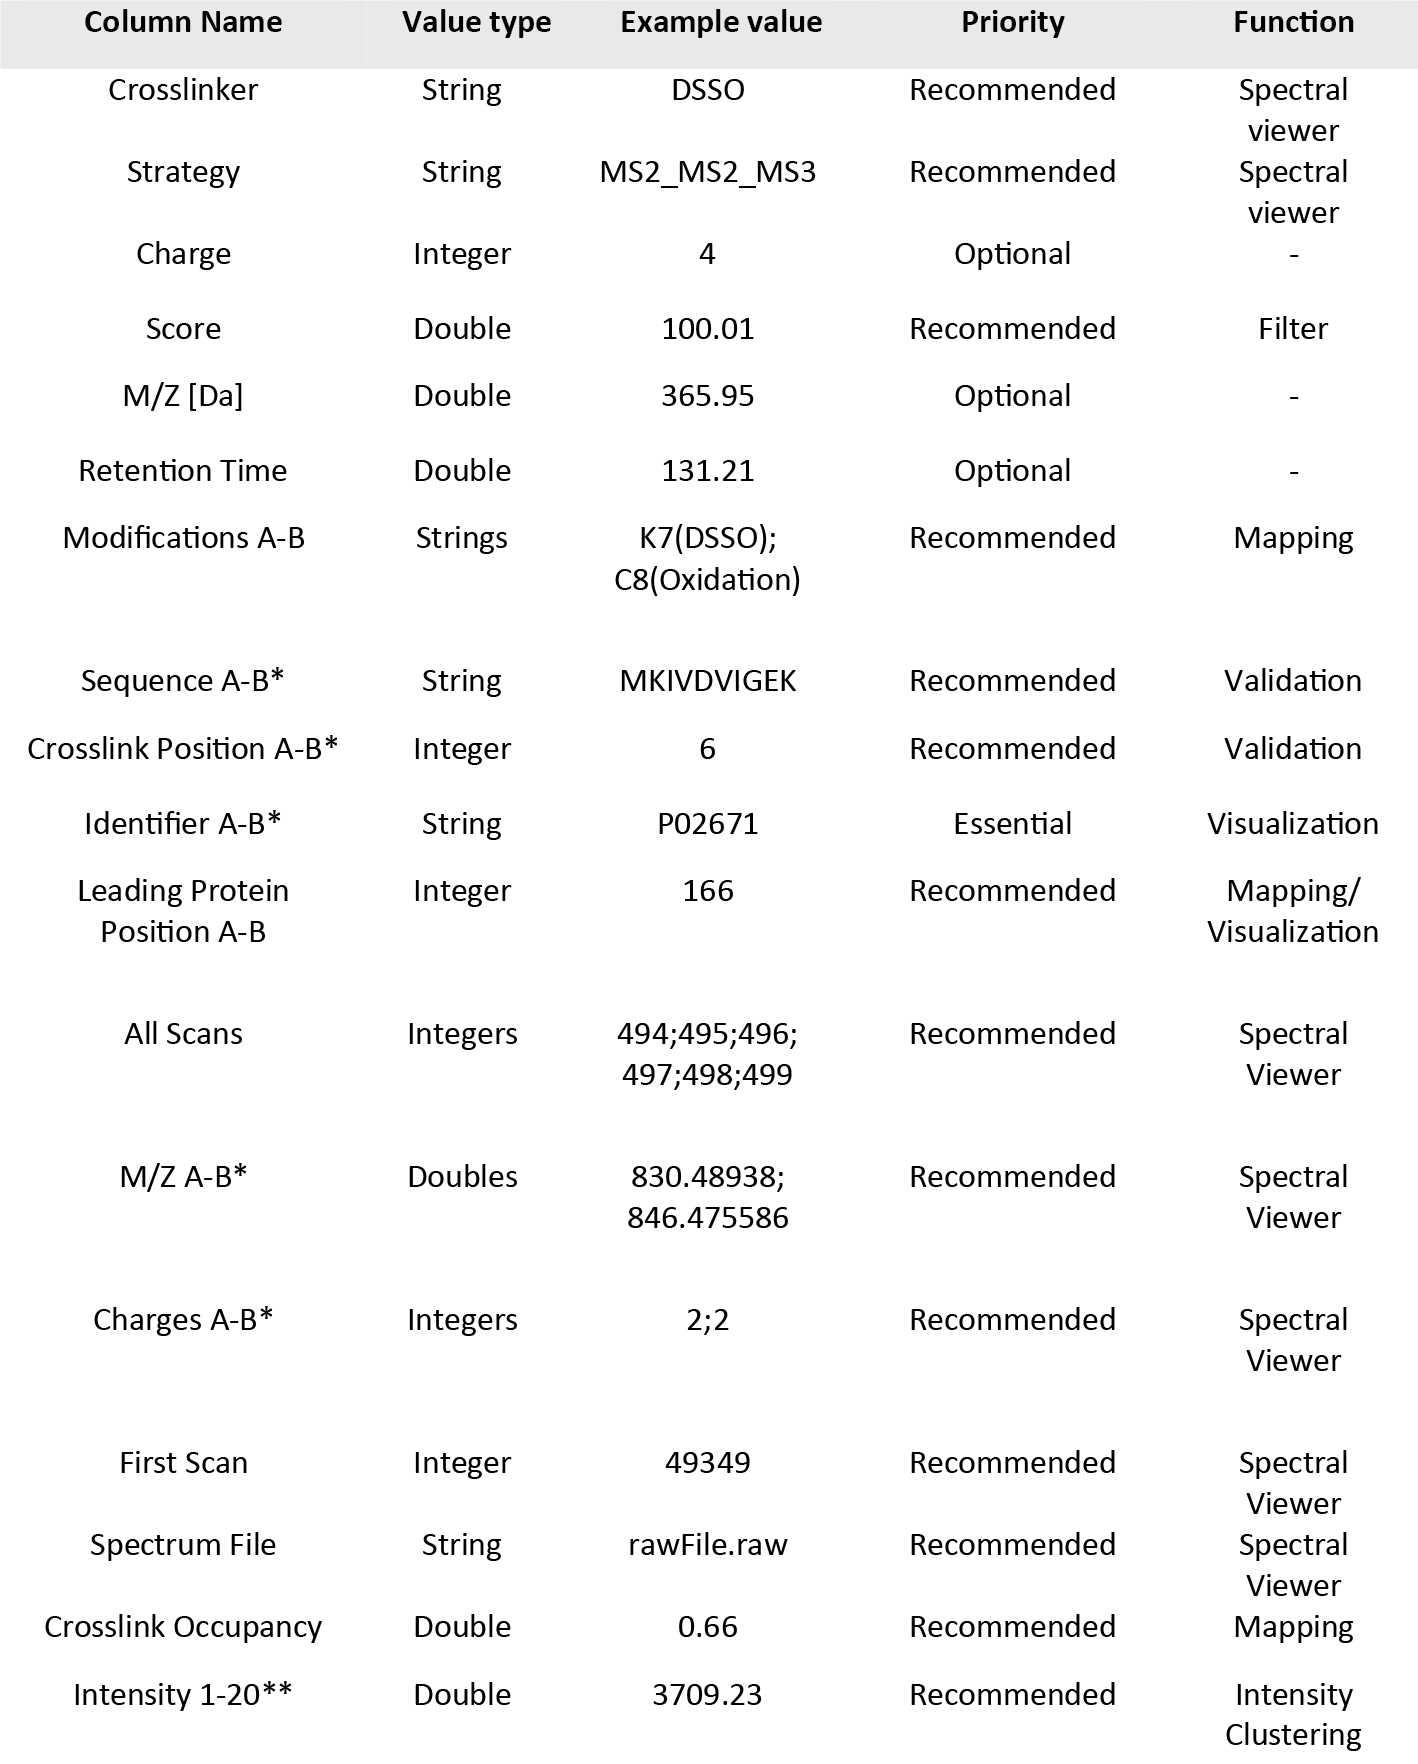
\includegraphics[]{Chapter.2/Figures/t2.png}
  \caption{
    \textbf{Recommended Input Format for Cross-ID}\textsuperscript{a}\\
    \textsuperscript{a}Optional columns were kept for the purpose of providing the user with additional information for inspection in tabular format and for exporting.\\
    \textsuperscript{b}Columns with a name indicating a range (e.g., charges A−B) indicate multiple columns with the same requirements. Columns needing an array of values (e.g., “all scans”) require those values to be separated by semicolons.\\
    \textsuperscript{c}Intensity columns are imported through a separate mechanism to avoid cluttering of the importer form. This means that the intensity columns should be named: intensity1, intensity2, and so on. Other column names do not require specific formatting as long as the importer is used.
  }
  \label{tab:tab2.2}
\end{table*}

To demonstrate the ability of Cross-ID to rapidly leverage quantitation information, we performed TMT labelling experiments on the bovine Protein Kinase A (PKA) complex. PKA is a tetramer composed of two regulatory subunits and two catalytic subunits. Each regulatory subunit is able to bind 2 molecules of cyclic AMP (cAMP), upon binding the catalytic subunits are released. We used TMT 10-plex to measure the structural behavior for increasing concentrations of cAMP. There are two types of regulatory subunits; for each type the alpha- and beta-forms are present and a complex can be formed either by combination of the alpha- and beta-forms or by one a single form. Catalytic subunits are also present as alpha- and beta-forms, but only one of the forms is present in the PKA complex. As the structure for the bovine type II alpha regulatory subunit is missing, we modelled this protein from residue 97 to 402 with I-TASSER \cite{yang2014i-tasser} (\textbf{Structure \ref{struct:structdummy2.1}}), using the available template from mouse (PDB ID 3TNP with resolution 2.3 Å, chain ~~b) . As structure with the bound cAMP ligand, we used a previously modelled structure from the SWISS-MODEL repository \cite{bienert2017swiss-model} (\textbf{Structure \ref{struct:structdummy2.2}}). We detect 5 intralinks for the type II regulatory subunit alpha-form (Uniprot accession P00515, \textbf{\autoref{fig:fig2.4}a}) and for the beta-form no crosslinks. The catalytic subunit is represented by the alpha subunit with 5 intralinks (Uniprot accession P00517, \textbf{\autoref{fig:fig2.4}a}). In both cases, it was possible to group the behavior of all detected crosslinks into 4 clusters even though the number of maximum clusters was set to 5 (see \textbf{\autoref{tab:tabdummy2.5}} and \textbf{\autoref{fig:figs2.1}a-d}).It is known that the regulatory subunit undergoes conformational changes upon binding of cAMP. Cluster 3 and 4 contain crosslinks with increasing intensities for increasing concentrations of cAMP. Crosslink 187-269 is mapped as 46.6 Å when no ligand is present (see \textbf{\autoref{fig:fig2.4}b}) and 21.0 Å with the ligand present (see \textbf{\autoref{fig:fig2.4}c}); for this crosslink we detect a 10-fold increase in intensity. Crosslink 342-376 is mapped as 21.2 Å on the holoenzyme regulatory subunit and quantified with relatively low intensity in the control experiment. On the folded conformation the same restraint is 30\% shorter and shows an intensity increase upon cAMP addition of almost 4–fold. There is one unmapped crosslink between lysine residues 315, which is located on the surface exposed flexble loop and might belong to an alternative folded conformation of the complex. Notably, the remaining crosslinks are mapped within the DSSO crosslinking range for at least one of the conformations of the regulatory subunit (\textbf{\autoref{tab:tabdummy2.6}}). The catalytic subunit is released upon cAMP binding and with this release cteayes a highly dynamic protein with domains involved in hinge and shear motions \cite{akamine2003dynamic}. Even though it is expected that this protein is very flexible, all detected intra-links can be mapped on the available apoenzyme structure (PDB ID 5VI9 with resolution 1.9 Å, chain ~~a) within the DSSO maximum crosslinking distance (\textbf{\autoref{tab:tabdummy2.6}}). Crosslink 24-193 is located in cluster 1 (\textbf{\autoref{fig:figs2.1}e}) and shows a drastic decrease in intensity for higher concentrations of cAMP. This behavior is not readily explainable, but we hypothesize that upon substrate binding the protein is made structurally less flexible by formation of a salt-bridge between one of these lysines and Asp’162 (see \textbf{\autoref{fig:fig2.4}d}).
%%TODO caption overflows
\begin{figure*}[!htb]
  \center
  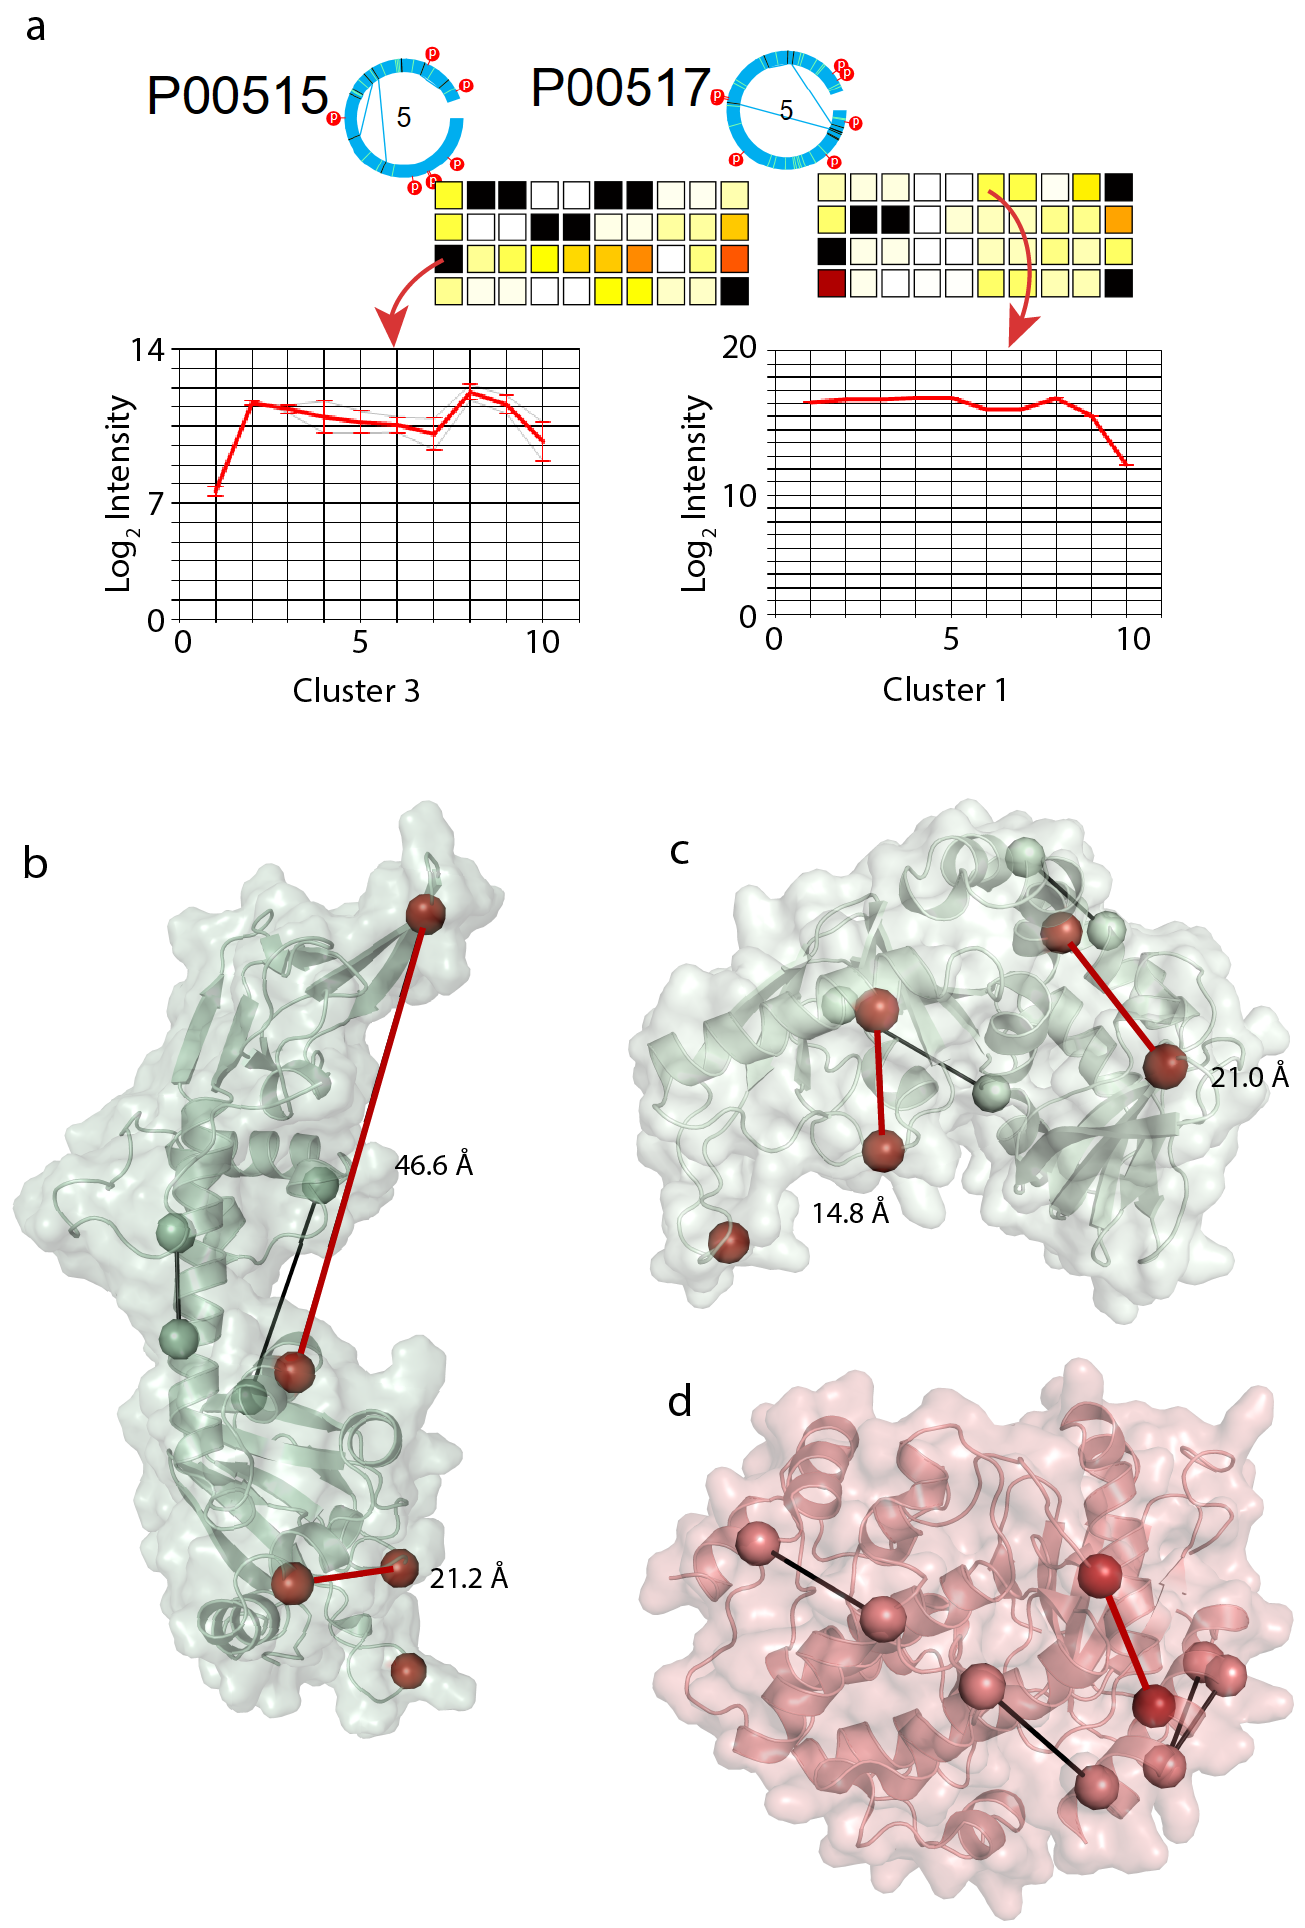
\includegraphics[]{Chapter.2/Figures/f5.png}
  \caption{
    \textbf{Quantitation with Cross-ID.} ~~a) Detected cross-links for the PKA complex in circular representation (left: regulatory subunit; right: catalytic subunit alpha). ~~b) Ligand-free and ~~c) cAMPbounded structures of bovine alpha type II regulatory subunit. ~~d)
    Structure of bovine catalytic subunit alpha with mapped cross-links. Cross-links mapped in black do not change intensity across TMT channels, whereas residues and cross-links mapped in dark red are changing their intensity across the TMT channels.
  }
  \label{fig:fig2.5}
\end{figure*}


\section{Conclusions}
Crosslinking mass spectrometry experiments tend to produce such large amounts of data, that processing rapidly becomes impractical – especially in the case of whole proteome experiments. To alleviate this we present Cross-ID, a tool that produces graph presentations of crosslinking data and offers several tools to bring the detected crosslinking data into structural data like crystal structures. It offers optimal integration with the XlinkX data analysis pipeline \cite{liu2017optimized, klykov2018efficient}, but also supports import of data in CSV format from other search engines with partial automation through a natural language importer. Various forms of grouping of the protein network are supported for gaining optimal insights in the detected data, with support for grouping on external data like e.g. GO annotations. To support analyses of the detected crosslinks on existing crystal structure data, Cross-ID implements automated sequence alignment to bridge the differences between the used sequences and those in the crystal structures. As further support in this direction, it also offers a convenient interface to the structural modeling pipeline of DisVis/HADDOCK. With support for various quantitation options with automated clustering, the tool provides a very detailed look at structures from a crosslinking point-of-view. Cross-ID was developed with extensibility in mind and as part of the XlinkX data analysis pipeline will see continued development and support. Future functionalities currently already under development include: integration of PPI databases such as String \cite{szklarczyk2015string} and CORUM \cite{ruepp2008corum:} to group based on known complexes, further integration with the HADDOCK software for structural modelling, implementation of true distance measures like e.g. Xwalk implements \cite{kahraman2011xwalk:}, integration with standardization efforts like mzIdentMl, and many others. To further integrate with other softwares, we aim to add support for non csv/text based output formats like pepXML \cite{hoopmann2016open} and/or pepXMLTab \cite{xiaojingwang2018pepxmltab:}.

\subsection{Acknowledgements}
We thank all Heck-group members for their helpful contributions and enduring early testing. From the Bonvin-lab we thank Alexandre Bonvin and Jörg Schaarschmidt for integration with the DisVis platform. From Thermo Fisher Scientific we thank Bernard Delanghe, Kai Fitzemeier and Frank Berg for their collaboration on incorporating the XLinkX crosslink search engine into the Proteome Discoverer software and Rosa Viner for her collaborative work on DSSO crosslinking and support in mass spectrometry method development. We acknowledge financial support by the large-scale proteomics facility Proteins@Work (Project 184.032.201) embedded in the Netherlands Proteomics Centre and supported by the Netherlands Organization for Scientific Research (NWO). Additional support came through the European Union Horizon 2020 program FET-OPEN project MSmed (Project 686547), and the European Union Horizon 2020 program INFRAIA project Epic-XS (Project 823839).

\subsection{Author contributions}
R.A.S. conceived of the study. O.K. performed the XL-MS experiments and provided ideas for features. S.C.d.G., H.v.d.T., and R.A.S. programmed Cross-ID. S.C.d.G., O.K. and R.A.S. wrote the paper, whereafter all authors critically read and edited the manuscript.

\clearpage
\begin{subappendices}
  \beginsupplement

  \section{Supplementary material}
  Supplementary Structure 1-2, Supplementary Result 1-2 and Supplementary Table 1 and 5-6 can be found online at:\\
  \emph{https://pubs.acs.org/doi/full/10.1021/acs.jproteome.8b00725}\\
  The Cross-ID software, documentation and instructional video can be found online at:\\
  \emph{https://www.hecklab.com/software/xlinkx}\\
  \refstepcounter{table}
  \label{struct:structdummy2.1}
  \refstepcounter{table}
  \label{struct:structdummy2.2}
  \addtocounter{table}{-2}
  \refstepcounter{table}
  \label{tab:tabdummy2.1}
  \addtocounter{table}{3}
  \refstepcounter{table}
  \label{tab:tabdummy2.5}
  \refstepcounter{table}
  \label{tab:tabdummy2.6}
  \addtocounter{table}{-6}

  \begin{figure*}[!hbt]
    \center
    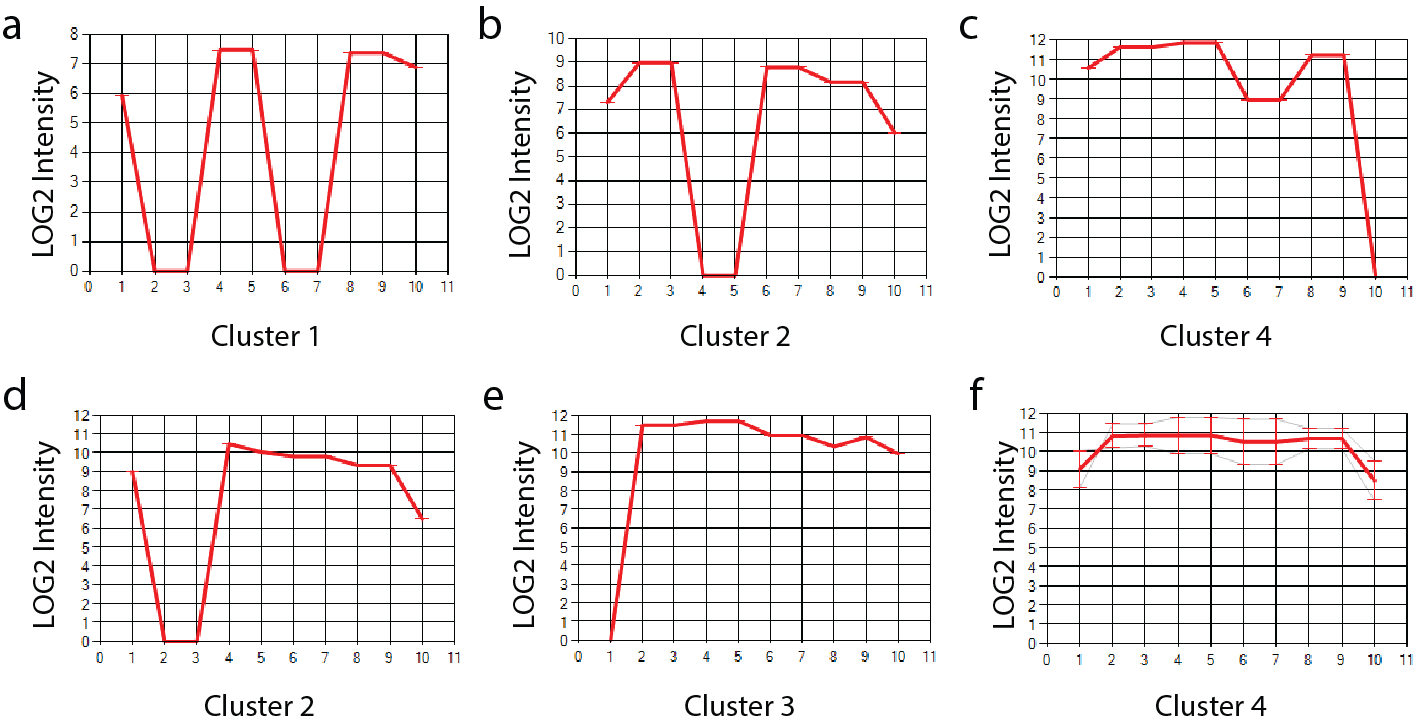
\includegraphics[]{Chapter.2/Figures/fs1.png}
    \caption{
      \textbf{Intensity clusters generated with Cross-ID for TMT-labelled crosslinked peptides of Protein Kinase A proteins.} TMT channels 1 to 10 corresponds to increasing concentration of cAMP ligand from 0 µM for channel 1 and 10 µM for channel 10. (A-D) Crosslinks intensity for bovine type II regulatory subunit alpha. (E-F) Crosslinks intensity for bovine catalytic subunit alpha.
    }
    \label{fig:figs2.1}
  \end{figure*}
  \vspace{1cm}
  \begin{table*}[!hbt]
    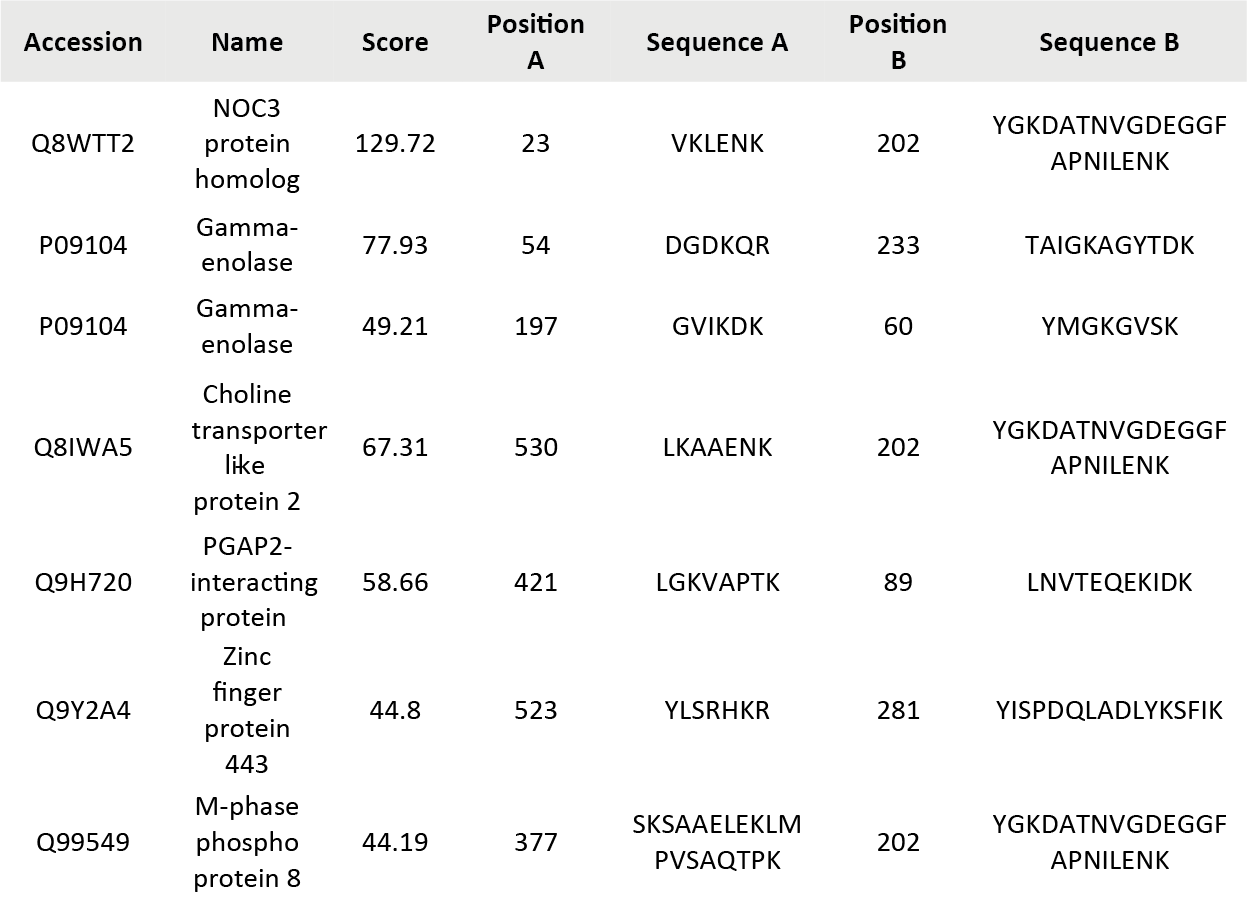
\includegraphics[]{Chapter.2/Figures/ts1.png}
    \captionsetup{singlelinecheck = false, format= hang}
    \caption{
      \textbf{Detected and mapped interlink-crosslinks for Alpha-Enolase.}
    }
    \label{tab:tabs2.1}
  \end{table*}
  \vspace{1cm}
  \begin{table*}[!hbt]
    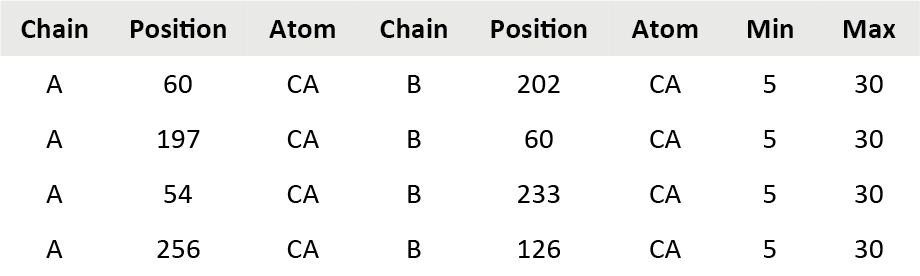
\includegraphics[]{Chapter.2/Figures/ts2.png}
    \captionsetup{singlelinecheck = false, format= hang}
    \caption{
      \textbf{DisVis input example file for potentially intersubunit Alpha-Enolase crosslinks.}
    }
    \label{tab:tabs2.2}
  \end{table*}
  \vspace{1cm}
  \begin{table*}[!hbt]
    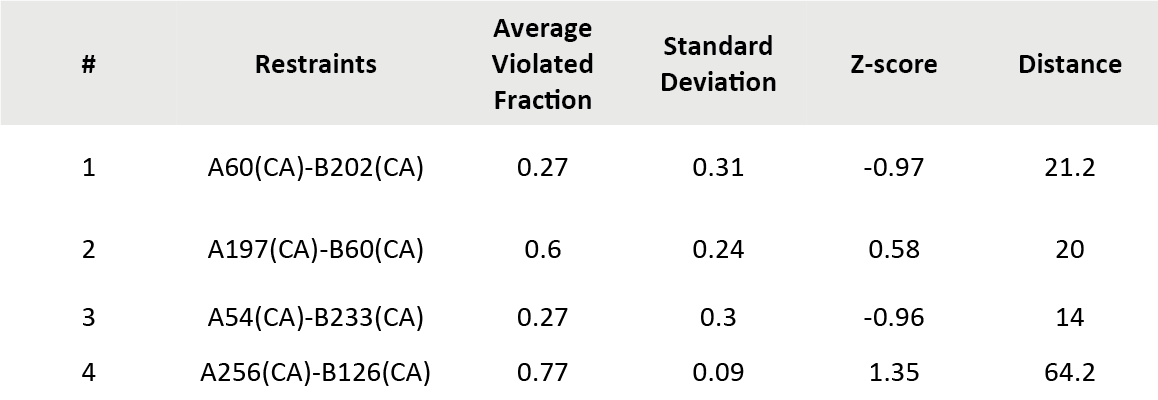
\includegraphics[]{Chapter.2/Figures/ts3.png}
    \captionsetup{singlelinecheck = false, format= hang}
    \caption{
      \textbf{DisVis output example for potentially intersubunit Alpha-Enolase crosslinks.}
    }
    \label{tab:tabs2.3}
  \end{table*}
\end{subappendices}

\clearpage
\section*{References}
\bibliographystyle{Stylesettings/pnas}
\patchcmd{\thebibliography}
{\clubpenalty 4000\widowpenalty 4000}
{\clubpenalties 1 10000 \widowpenalties 1 10000}
{}{}
\bibliography{chapmerge}
\stopthumb


\picturechapter{Human plasma IgG1 repertoires are simple, unique, and dynamic}{Chaptercovers/ch3.pdf} \label{ch-3}
\vspace*{0.25cm}

{\footnotesize Albert Bondt, Max Hoek, Sem Tamara, Sebastiaan C. de Graaf, Weiwei Peng, Douwe Schulte, Danique M.H. van Rijswijck, Maurits A. den Boer, Jean-François Greisch, Meri R.J. Varkila, Joost Snijder, Olaf L. Cremer, Marc J.M. Bonten, Albert J.R. Heck}

\begin{center}
  \vspace{1cm}
  \includegraphics[]{Chapter.3/Figures/ch3a.png}
  \vspace{0.25cm}
\end{center}

\begin{flushleft}
  \vspace*{\fill}
  \rule{\textwidth}{1pt}\\[0cm]
  \textbf{This chapter is based on work in the following publication:}\\
  \footnotesize
  \textbf{\emph{Cell Systems}} (2021), 12:1131-1143, doi:10.1016/j.cels.2021.08.008\\
  \footnotesize
\end{flushleft}
%%Abstract
\begin{abstract102}
  Although humans can produce billions of IgG1 variants through recombination and hypermutation, the diversity of IgG1 clones circulating in human blood plasma has largely eluded direct characterization. Here, we combined several mass-spectrometry-based approaches to reveal that the circulating IgG1 repertoire in human plasma is dominated by a limited number of clones in healthy donors and septic patients. We observe that each individual donor exhibits a unique serological IgG1 repertoire, which remains stable over time but can adapt rapidly to changes in physiology. We introduce an integrative protein- and peptide-centric approach to obtain and validate a full sequence of an individual plasma IgG1 clone \emph{de novo}. This IgG1 clone emerged at the onset of a septic episode and exhibited a high mutation rate (13\%) compared with the closest matching germline DNA sequence, highlighting the importance of \emph{de novo} sequencing at the protein level.
\end{abstract102}
%%Main Text
\thumbforchapter

\section{Introduction}
\lettrine[lraise=0.1, nindent=0em, slope=-.5em]{T}{he}
human immune system protects us not only from threats posed by pathogens but also cancer and various other diseases. The immune response in health and disease is crucially dependent on each person’s repertoire of immune cells, antibodies, and other circulating plasma proteins. A detailed molecular view of these plasma components is crucial to understanding how they affect each individual’s immune response. Immunoglobulins (Igs) represent some of the most important molecules in the human immune system. Ig molecules consist of two identical heavy chains and two identical light chains, held together by a network of disulfide bridges. The heavy chains possess three (IgG, IgA, and IgD) to four (IgM and IgE) immunoglobulin domains with large, conserved regions, which play a role in receptor binding and complement activation. Similar to the heavy chain, the C-terminal domain of the light chain is constant. On the other hand, for both heavy and light chain, the sequence of the N-terminal Ig domains is hypervariable and contains the recognition-determining parts, better known as complementarity-determining regions (CDRs), of the molecule. They are enclosed in the two fragment antigen-binding (Fab) arms of the antibody, consisting of the light chain and the N-terminal parts of the heavy chain (Fd).
The variable regions of the antibody, in particular the CDRs, are optimized to recognize antigens by a process known as affinity maturation. The best antigen binders, modified through somatic recombination and hypermutation of numerous coding gene segment variants, give rise to the mature IgG secreting plasma B cells that produce the antibodies that end up in our circulation. The circulating antibodies, thus, consist of the fully matured heavy- and light-chain variable domain sequences that harbor the CDRs, joined by generally less sequence-variable framework regions (FR). Each unique combination of mature chains is called an Ig clone.
Considering the genes encoding the variable domain sections and the known genomic rearrangements, somatic hypermutations, and post-transcriptional processes that join these sections—resulting into the ultimate protein products—it has been estimated that in humans the theoretical molecular Ig diversity may extend beyond 10\textsuperscript{15} \cite{schroeder2006similarity}. Not all theoretically possible Ig clones will be expressed in the human body, since the number of B cells in a human body is several orders of magnitude lower (1–2 × 10\textsuperscript{11}) \cite{apostoaei2012review}. Nevertheless, it has been assumed that the actual repertoire of circulating Igs is extremely large and diverse \cite{briney2019commonality, soto2019high}.
Recombinantly expressed clones (mainly IgG) have become a major class of therapeutics, used to fight multiple types of pathologies such as cancers and various infectious diseases. Recent developments have moved the field toward using therapeutic monoclonal antibody (mAb) sequences derived from human subjects instead of laboratory animals; this trend is exemplified by successful new treatments for Ebola \cite{corti2016protective, dyer2019two, mulangu2019randomized} and COVID-19 \cite{jones2021neutralizing}. These therapeutic antibody sequences are inferred from genetic material recovered from patients that successfully overcame the disease. The ability to detect and identify individual mature IgG protein sequences directly from donor specimens would aid such efforts.
To experimentally determine the Ig repertoire, attempts have been made to sequence Ig nucleic acids from bulk B cell populations or B cell subsets from single donors. These Igs are analyzed with high-throughput sequencing (Ig-seq or Rep-seq) at the DNA or RNA level \cite{georgiou2014promise}, resulting in datasets of tens to hundreds of thousands of unique reads of variable abundance \cite{vollmers2013genetic}. Unfortunately, these analyses at the level of DNA and RNA do not measure the actual antibodies of interest, and the presence of a cognate BCR sequence in the B cell population provides no information regarding abundance levels of the antibodies that end up in circulation.
Alternatively, the challenge could be approached from the protein level, analyzing the Ig repertoire present in circulation. The most abundant Ig in human plasma is IgG, at a concentration of approximately 10 mg/mL during health \cite{cassidy1975human, gonzalez-quintela2008serum}. Of the four IgG subclasses, IgG1 is the most abundant, accounting for more than 50\% of all IgGs \cite{giessen1975quantification} in most people. Given the extremely high theoretical limits on Ig diversity and the large number of experimentally determined variants, most researchers have refrained from analyzing plasma antibodies directly at the protein level. It has been mostly assumed that it is impossible to detect any single Ig clone against the expected background of thousands to millions of other clones.
However, in recent years, several attempts have been made to identify plasma Igs directly. G. Georgiou and colleagues should be considered pioneers. In their method (also referred to as Ig-seq, but protein-based instead of solely gene-based), IgGs are purified from plasma, and tryptic Ig peptides are characterized using liquid chromatography coupled online to tandem mass spectrometry (LC-MS/MS), focusing on the detection of IgG heavy-chain CDR3 peptides \cite{chen2017proteomic, lavinder2014identification, lee2016molecular-level, lee2019persistent, wine2013molecular}. Another recently developed proteomics approach uses LC-MS to profile intact light chains purified from plasma \cite{barnidge2014phenotyping, barnidge2014using, he2019classification, he2017analysis, mills2015detecting, sharpley2019novel}. In another report, profiling and sequencing of intact Fabs was attempted, but the sensitivity was too low, and only a few sequence tags could be derived from separated light chains \cite{wang2019top-down}.
In these approaches, information about the heavy- and light-chain pairing is often lost, which is unfortunate as only the combined CDRs from both heavy and light chain provide the full complementarity against an antigen. Of note, in nearly all these studies, only a subset of plasma immunoglobulins recognizing and binding a specific antigen was targeted, or a mAb spiked into plasma was used as a model. Nevertheless, the remarkable observation was made that a person’s plasma Ig repertoire could be several orders less variable than assumed based on the available B cell repertoire and likely dominated by only a limited number of clones. Whether this observed number of IgGs is a consequence of the targeted analysis of antigen-specific IgGs or diseases with monoclonal IgG overexpression (gammopathy) remained unclear.
Here, we introduce a sensitive and efficient approach for quantitative plasma IgG1 clone profiling. The method was applied to a sample set of two healthy control donors, as well as eight critically ill patients, from which sequential plasma samples were retrieved while developing nosocomial sepsis, experiencing a dramatic immunological change in a relatively short time span (\textbf{\autoref{fig:fig3.1}a}). The application of our method revealed several important properties of the human plasma IgG1 repertoire: (1) the total IgG1 repertoire is dominated by a few dozen clones, but (2) is unique for each individual, and (3) single clones are differentially affected by physiological changes. Next, as proof of concept, we \emph{de novo} sequenced a single plasma clone—that appeared at sepsis onset—directly from human plasma, only made possible by using iteratively a combination of protein-centric and peptide-centric proteomics. To validate the correctness of the derived \emph{de novo} IgG1 sequence, we produced its recombinant mAb equivalent and compared its key structural features with the plasma clone. We foresee that this approach will unlock the potential of mass spectrometric analysis and identification of disease-responsive IgGs that may be directly evaluated and used as therapeutic agents, as they do already represent fully matured, fully human Abs.
\begin{figure*}[!htb]
  \center
  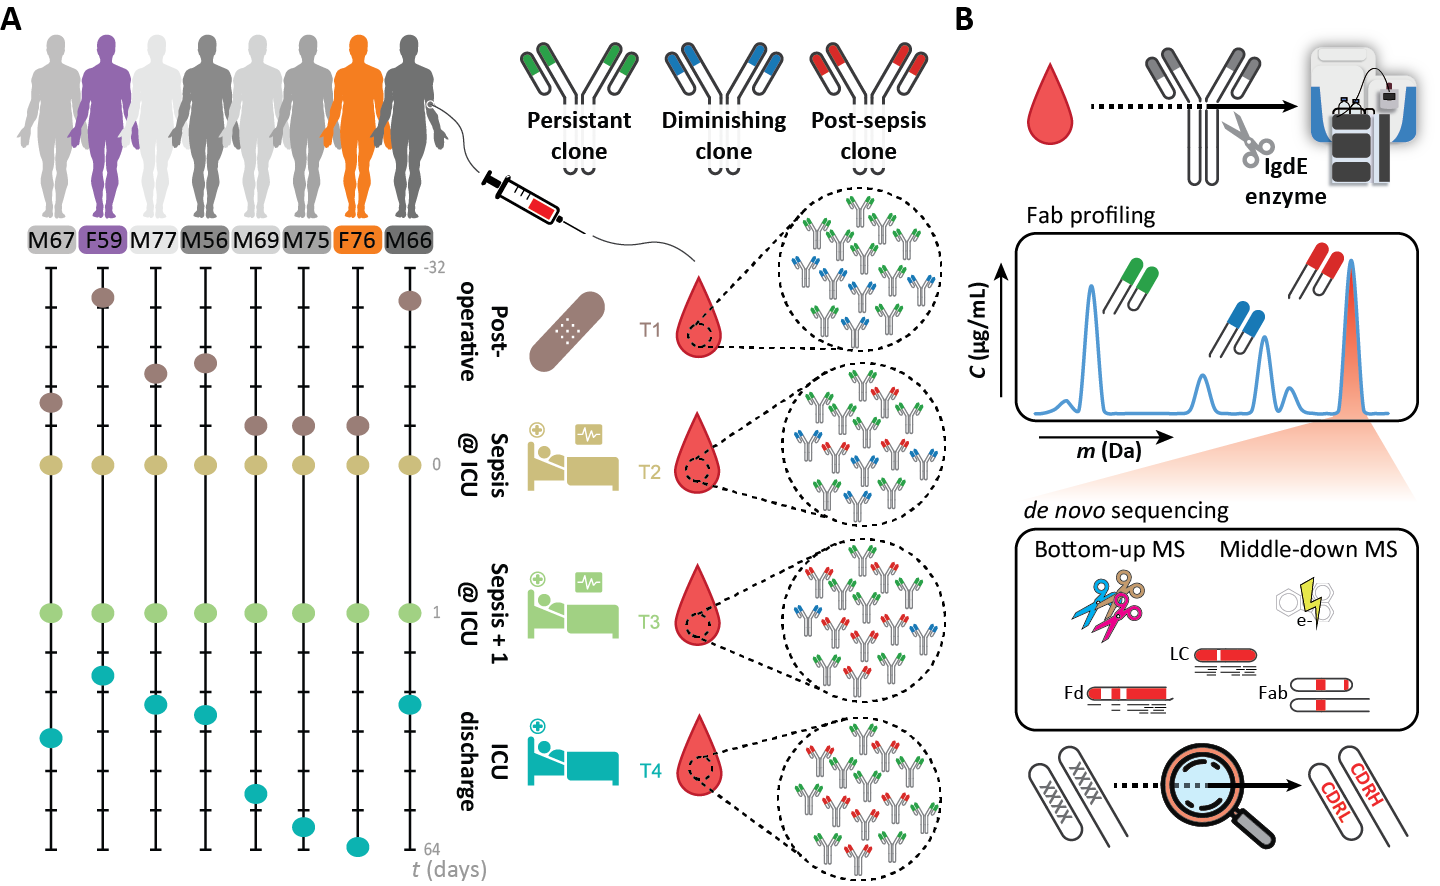
\includegraphics[]{Chapter.3/Figures/f1.png}
  \caption{
    \textbf{Monitoring individual plasma IgG1 profiles.} ~~a) Longitudinal analysis of the IgG1 repertoire from sepsis patient plasma obtained at four time points, reveals its simplicity and clonal dynamics: some clones are fairly constant (green), some disappear (blue), whereas others appear over time (red). ~~b) The experimental approach taken involves IgG capturing from 10–100 μL of serum, followed by the specific enzymatic digestion of the IgG1 molecules in their hinge region, generating two identical Fab portions. All generated Fabs are collected and subsequently subjected to LC-MS analysis. The clonal repertoire is profiled, whereby each identified clone is characterized by its unique mass and retention time. A single post-sepsis clone from one of the patients (F59) was selected for \emph{de novo} sequencing, combining protein- and peptide-centric mass-spectrometry-based sequencing. The extracted full sequence of the plasma IgG1 was validated by analyzing, in a similar manner, a recombinant IgG1 analog of the plasma clone.
  }
  \label{fig:fig3.1}
\end{figure*}


\section{Results}

\subsection{Mass-spectrometry-based Fab profiling of the human plasma repertoire}
To chart and monitor the nature of the plasma IgG1 repertoire, we started our analysis with 10 μL of plasma, derived from a single donor. From such a sample, we first captured all intact IgGs using affinity beads. Subsequently, the captured IgG molecules were digested using the highly specific Ig degrading enzyme (IgdE), cleaving specifically IgG1’s at a defined site in the upper hinge region, resulting in the segregated Fc (that remains bound to the affinity beads) and two identical Fabs (\textbf{\autoref{fig:fig3.1}b}) \cite{spoerry2016novel}. We focused on the Fab fragments derived from the intact IgGs because this (1) concentrates the clonal signal since each IgG1 provides two identical Fab molecules, (2) results in more homogeneous mass profiles by removing the Fc portions that harbor two heterogeneous N-glycosylation sites, and (3) retains all hypervariable CDRs, which define the unique identity and antigen recognition of each clone.
Following elution of the IgG1 Fabs, all these intact 45–53-kDa Fab molecules were subjected to reversed-phase LC-MS. All individual Fab fragments were subsequently characterized by their distinctive mass and chromatography retention time. In our analyses, we spiked-in two monoclonal IgG1 antibodies (\textbf{Data \ref{tab:tabdummy3.1}}, mAbs \#1 and \#2) of known sequence at a defined concentration. These mAbs were used as internal standards for mass and retention time calibration and quantification of all the other distinctive plasma IgG1 clones. This also allowed us to calculate the precision and accuracy of retention time, mass, and quantification in our measurements as illustrated in \textbf{\autoref{fig:figs3.1}a}.
Using a mixture of six monoclonal antibodies (\textbf{Data \ref{tab:tabdummy3.1}}) spiked into a single-donor plasma background, we furthermore observed linear relationship between (1) the quantity of mAbs that were spiked into the plasma sample, and (2) the quantity that is observed (R\textsuperscript{2} = 0.99, \textbf{\autoref{fig:figs3.1}b}), using a dilution/titration with 4,000, 800, 200, and 20 ng per mAb. Of note, no discrepancy was observed for the Fab glycosylated mAb as compared to the other mAbs. To evaluate the repeatability (technical replicate and sample preparation replicate), the 100 most abundant plasma-derived clones in this sample were quantified in multiple replicates (\textbf{\autoref{fig:figs3.1}c}). Finally, one of the samples was injected three times to serve as injection replicates (\textbf{\autoref{fig:figs3.1}c}, \#1). From all these validation experiments, we concluded that, by using the approach depicted here (\textbf{\autoref{fig:fig3.1}}), the repertoire of Fab clones could be accurately and reproducibly determined from as little as 10 μL of plasma obtained from a single donor at a single time point.

\subsection{Plasma IgG1 repertoires are dominated by a few clones}
Next, we analyzed in parallel a set of 32 plasma samples obtained from eight patients of the Dutch molecular diagnosis and risk stratification of sepsis (MARS) cohort (\textbf{\autoref{fig:fig3.1}a}; \textbf{Data \ref{tab:tabdummy3.2}}). All these patients underwent major gastrointestinal surgery and subsequently developed an infectious complication (i.e., anastomotic leakage or pneumonia) resulting in sepsis. Plasma samples were obtained from the patients at four different stages: within 24 h of surgery when no signs of sepsis were present (sample T1; between t = −19 and t = −2 days), on two consecutive days after onset of sepsis (samples T2 and T3; t = 0 and t = 1 day), and upon intensive care unit (ICU) discharge, when the sepsis had been resolved (sample T4; between t = 3 and t = 61 days) (\textbf{\autoref{fig:fig3.1}a}). In addition, to monitor the nature of the plasma IgG1 repertoire in healthy donors, we performed an identical analysis on two sets of three sequential healthy donor plasma samples, each collected roughly 1 month apart.
In marked contrast to expectations of extensive IgG1 diversity, we observed that all the LC-MS profiles of IgG1 Fab molecules were dominated by just a few dozen peaks, both in the 32 sepsis plasma samples as well as in the six plasma samples of the healthy donors (\textbf{Data \ref{data:datadummy3.1} and \ref{data:datadummy3.2}}). In each of the LC-MS runs, we could pick up distinctive IgG1 signals of between 35 and 543 in abundance dominant clones (median 196; \textbf{Data \ref{data:datadummy3.1}}) that we distinguished by their masses in Dalton and retention times (RT) in minutes. Each detected clone was given a unique identifier: \textsuperscript{RT} \# \textsubscript{mass}.
We found that the summed concentrations of the 30 most abundant IgG1 clones account for more than two-thirds of all IgG1 molecules detected from plasma (median 71.8\%, range 47.3\%–98.3\%, \textbf{Data \ref{data:datadummy3.1}}). The full lists of detected clones are provided in \textbf{Data \ref{data:datadummy3.1}}. In addition, the deconvoluted mass plots (similar to \textbf{\autoref{fig:fig3.2}c}) and the raw chromatograms supported by extracted chromatograms for all identified Fabs obtained in the LC-MS measurements are provided in \textbf{Data \ref{data:datadummy3.2}}, and one example of the actual raw mass spectrometry data of Fabs that we have analyzed is provided in \textbf{Data \ref{data:datadummy3.3}}.


Next, we looked at the cumulative mass distribution of all detected IgG1 Fabs in the plasma samples from all donors and at all time points. This cumulative mass distribution—representing more than 5,500 clones experimentally identified—resembled the expected mass distribution of over 130 million IgG1 Fabs constructed from the sequences in the ImMunoGeneTics information system (IMGT) \cite{lefranc1999imgt} database (\textbf{\autoref{fig:figs3.1}d}), revealing that we profiled a representative IgG1 repertoire.

\begin{figure*}[!hp]
  \center
  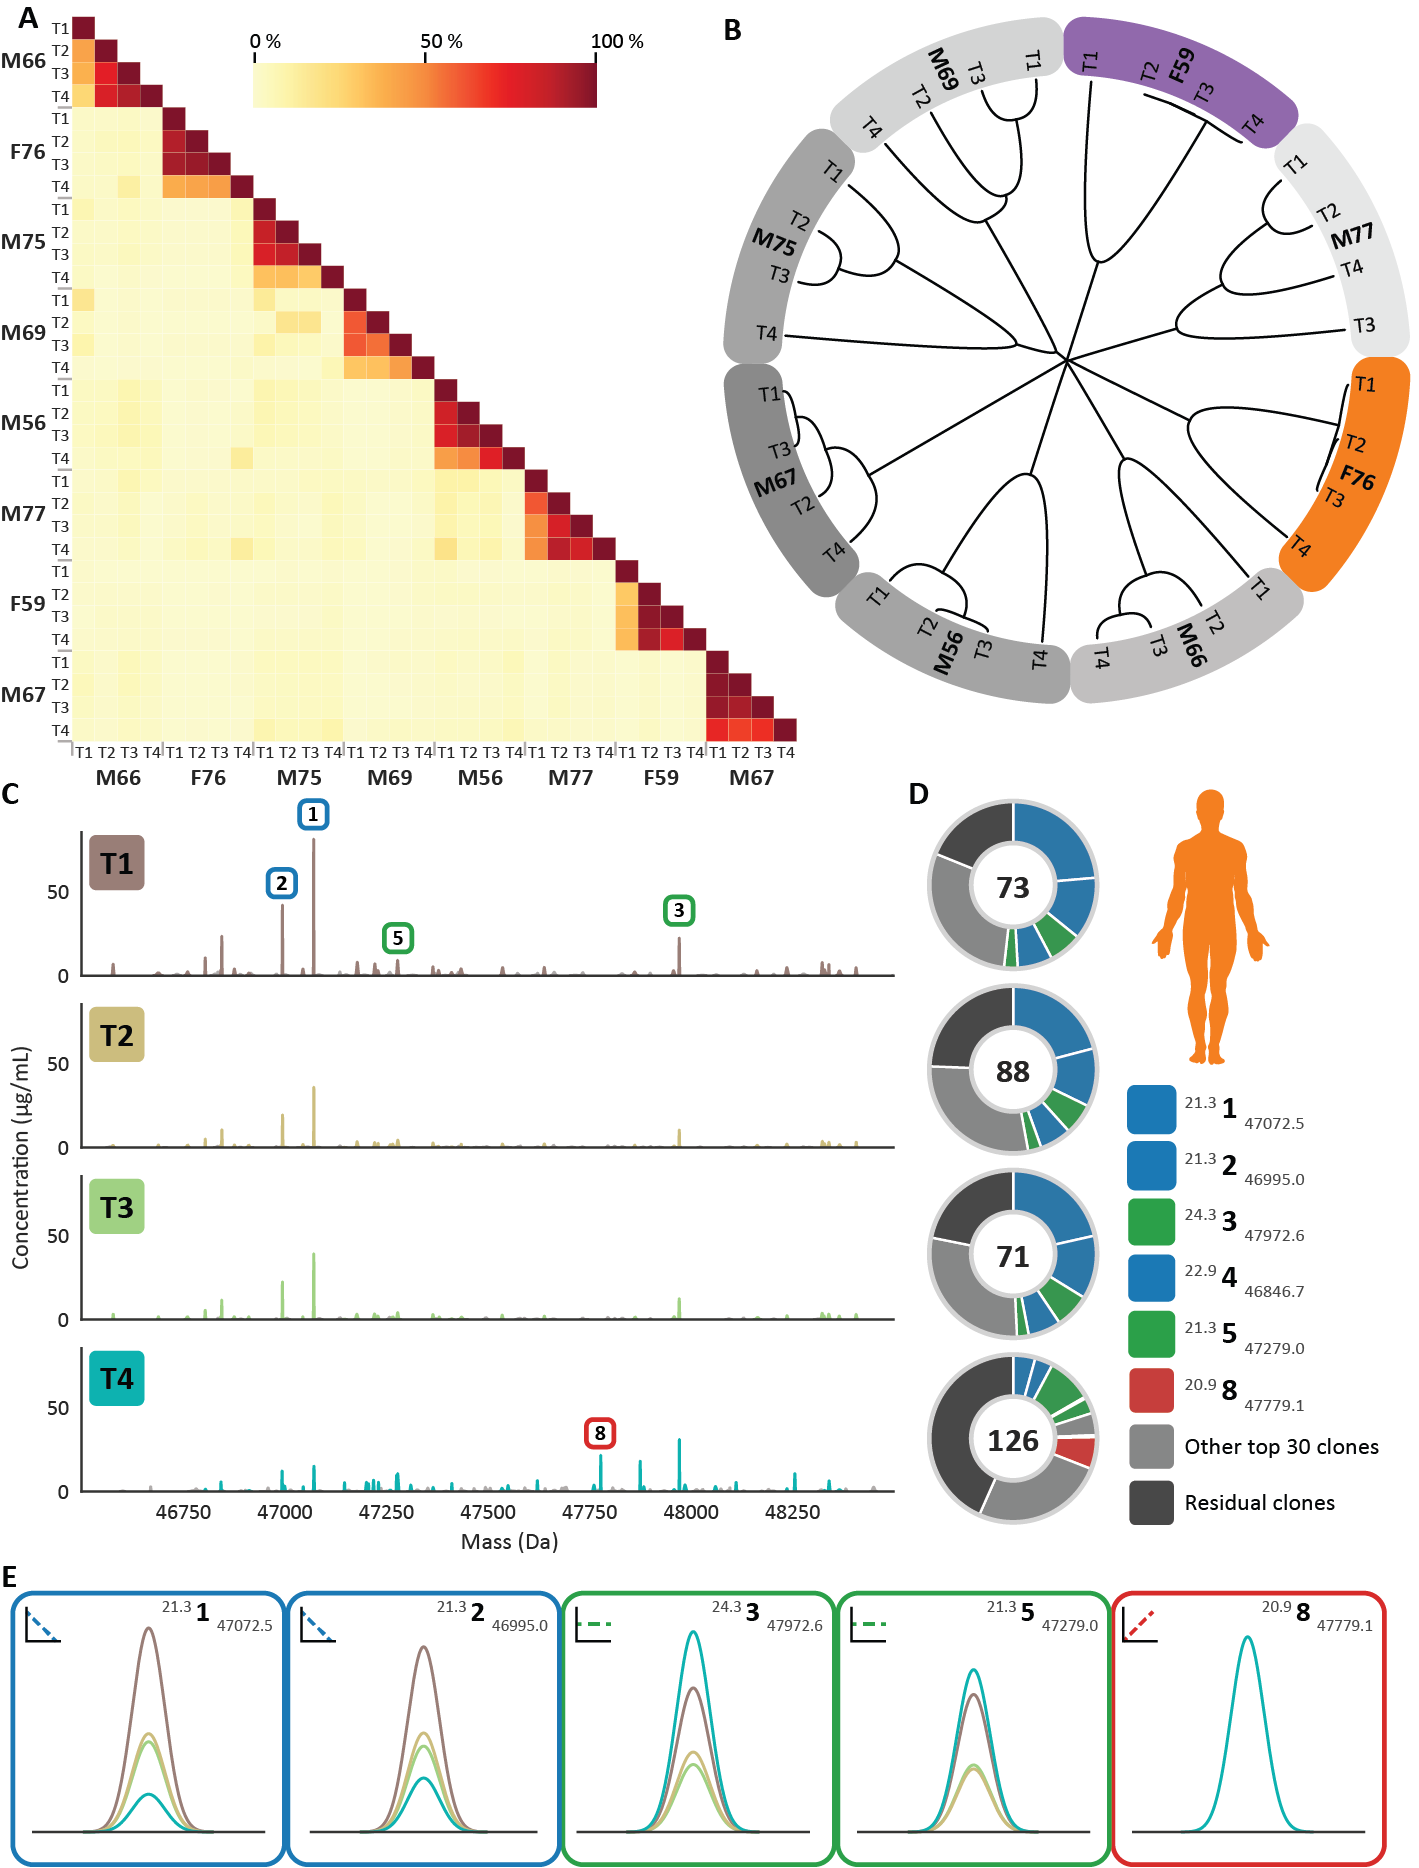
\includegraphics[]{Chapter.3/Figures/f2.png}
  \captionsetup{singlelinecheck = false, format= hang}
  \caption{
    Figure legend on next page.
  }
  \label{fig:fig3.2}
\end{figure*}
\addtocounter{figure}{-1}
\begin{figure*}[!ht]
  \caption{
    \textbf{Monitoring personalized plasma Fab repertoires reveals not only their simplicity and extreme donor uniqueness but also longitudinal clonal variations within a single donor.} ~~a) Heatmap illustrating the degree of overlap between the detected IgG1 repertoires in all analyzed sepsis patient plasma samples. For each of the eight donors, four sampling times were available, and Fab profiles were measured by LC-MS analysis. Each LC-MS peak, exhibiting a unique mass and retention time pair, was considered a unique clone and annotated as \textsuperscript{RT} \# \textsubscript{mass}. The amount of Fab molecules, based on intensity that is persistent, is quantified and shown as a percentage as indicated by the color bar. In between donors, the overlap is found to be on average 3\%, whereas within a single donor at different time points the overlap was found to be in between 26\% and 98\%. ~~b) Hierarchical clustering of the Fab clonal repertoires based on correlation distance. The branch lengths depict the distance between the repertoires. Donors are colored as in \textbf{\autoref{fig:fig3.1}a}. ~~c) Longitudinal deconvoluted Fab mass profiles of donor F76 at each of the four time points. Each peak represents a unique Fab at its detected mass and plasma concentration. The top 30 most intense Fab clones in each sample are colored reflecting the time points, the other clones are colored gray. Five peaks are highlighted with a box that is colored based on the longitudinal behavior of the Fab concentration in plasma (blue, diminishing clone; green, persistent clone; and red, post-sepsis clone), a magnified version of each of these Fab signals is shown in ~~e) . ~~d) Pie charts portraying the total number and distribution of clones in donor F76 for each time point. The value within the chart displays the number of identified unique Fab molecules. The five most intense Fabs are colored based on longitudinal behavior, and their mass and retention time are depicted in the legend in order of abundance. ~~e) Magnified mass plots for each of the highlighted clones. The peaks are colored according to the time points, the surrounding border and sign indicate the longitudinal behavior and the top right shows the annotated clone ID.
  }
\end{figure*}

As can be seen in \textbf{\autoref{fig:figs3.1}d}, most Fab fragments exhibit masses between 46 and 49.5 kDa. However, we also did detect some higher Fab masses, which may be indicative of Fab glycosylation. The average mass of Fab glycans is estimated to be around 2,300 Da \cite{bondt2016fab, hafkenscheid2017structural}. In two of our donors, annotated M66 and M77, we did detect relatively high levels of Fab glycosylation as shown for M66, time point 3, in \textbf{\autoref{fig:figs3.2}a}, with the annotation of the putative Fab glycosylation annotated in \textbf{\autoref{fig:figs3.2}b}. Still the Fab glycosylated clones represented just a few percent of the total abundance (2\%–6\% for donor M66 and M77). The fractional abundance of glycosylated Fabs in the other patients was between 0\% and 1.86\% (with a median of 0.295\%) (\textbf{\autoref{fig:figs3.2}c}). Also, in the two healthy donors, one displayed a fractional abundance of glycosylated Fabs of about 3\% (F66H), whereas in the other donor this remained around 0.5\% at all sampling time points. This fractional abundance is substantially lower than would be predicted based on the IMGT database ($\sim$11\% of these 130 million sequences carry at least one consensus N-glycosylation site) and lower than the $\sim$17\% described in literature \cite{bondt2016fab, hafkenscheid2017structural}. However, our data reveal that the fractional abundance of glycosylated Fabs is also donor-dependent.

\subsection{Plasma IgG1 repertoires are unique for each donor}
Next, we compared the IgG1 Fab profiles between time points not only within a single donor but also between different donors. Interindividual analyses showed that virtually none of the Fab IDs overlapped between individuals (\textbf{\autoref{fig:fig3.2}a, \autoref{fig:figs3.3} and \autoref{fig:figs3.4}a and b}). Also, hierarchical clustering based on clone IDs clusters each donor distinctively (\textbf{\autoref{fig:fig3.2}b}). Thus, each donor has its own simple albeit unique IgG1 repertoire. However, within each individual, overlap between the measured IgG1 repertoires measured across time was found to be very high, even when the time span largely exceeded the average half-life of IgG1s (\textbf{\autoref{fig:fig3.2}a–d and \autoref{fig:figs3.4}}). A large portion of the most abundant IgG1s remains present throughout the sampling window of up to 2 months, although we also observe a response in the IgG1 profile due to changes in the patient’s physiology (discussed below). To exclude whether these findings were due to the severe physiological state of the eight septic patient donors, we performed a similar analysis on plasma of two healthy donors. In the absence of a dramatic immunological challenge, the IgG1 profiles, as obtained from the two healthy donors, show (1) a very high stability over time within individuals and (2) an interindividual overlap in uniquely RT- and mass-identified IgG1 clones near to zero (\textbf{\autoref{fig:figs3.4}a and b}).

\subsection{Longitudinal quantitative monitoring of single IgG1 clones}
By spiking in two recombinant IgG1 mAbs at a known concentration to the plasma samples prior to sample preparation, we could provide additional absolute quantification for the abundance of the detected IgG1s. The concentrations of the LC-MS-detected endogenous IgG1 clones present in plasma ranged from less than 0.05 up to >400 μg/mL (<300 pM up to >2.5 μM, median $\sim$6.25 nM; \textbf{Data \ref{data:datadummy3.1}}). Monitoring serological IgG1 repertoires over time in patients who had undergone a septic episode, we observed several distinct quantitative patterns. The most recognizable patterns are highlighted in \textbf{\autoref{fig:fig3.2}c–e}. There are IgG1 clones that become lower in concentration over time (\textbf{\autoref{fig:fig3.2}c–e}, blue boxes). Another category of IgG1 clones was undetectable in the plasma until post-sepsis but became abundantly present at T4 (\textbf{\autoref{fig:fig3.2}c–e}, red boxes). Yet, another group of IgG1 clones was found to be rather persistent in concentration over all sampling moments (\textbf{\autoref{fig:fig3.2}c–e}, green boxes). In healthy donors, the majority of clones were more persistent in concentration, although some subtle changes could be observed for some clones.

\subsection{Full \emph{de novo} sequencing of an individual plasma IgG1 clone}
From the data presented earlier, we can conclude that the plasma IgG1 repertoire of individual healthy and diseased donors is unique and dominated by a few dozen abundant clones. Next, we sought to identify the exact sequences of these clones to obtain further insight into their function and origin. Complete \emph{de novo} sequencing of serological IgGs is notably difficult for several reasons. First, the inherent sequence hypervariability has so far proven to be highly challenging even when (personalized) genome-based sequence templates are available. Second, \emph{de novo} sequencing of antibodies at the protein level by MS is hampered by the complex nature of IgG molecules, stemming from their multichain structure and the intricate network of disulfide bridges. Finally, although shotgun proteomics can be used to obtain (partial) sequences of purified mAbs \cite{guthals2017de, sen2017automated, tran2016complete}, this becomes several orders of magnitude more difficult in a plasma background containing many IgG molecules of closely homologous sequences.
To tackle this challenge, we explored a hybrid and iterative approach combining state-of-the-art peptide-centric (i.e., bottom-up) and protein-centric (i.e., middle-down) mass-spectrometric sequencing methods, using dedicated algorithms to mix-and-match the extracted proteomics-based sequencing data. As proof of concept, we attempted to fully sequence the light and heavy chain of a Fab derived from a single highly abundant IgG1 clone observed in donor F59. This donor showed a plasma IgG1 repertoire dominated by two clones in particular: \textsuperscript{24.4} 1 \textsubscript{47,359.4} (average mass 47,359.4 Da, retention time 24.4 min) and \textsuperscript{20.6} 2 \textsubscript{47,025.7} (\textbf{\autoref{fig:fig3.3}a}). We focused on the \textsuperscript{24.4} 1 \textsubscript{47,359.4} clone, as this clone appeared exclusively after the onset of sepsis.

\begin{figure*}[!hptb]
  \center
  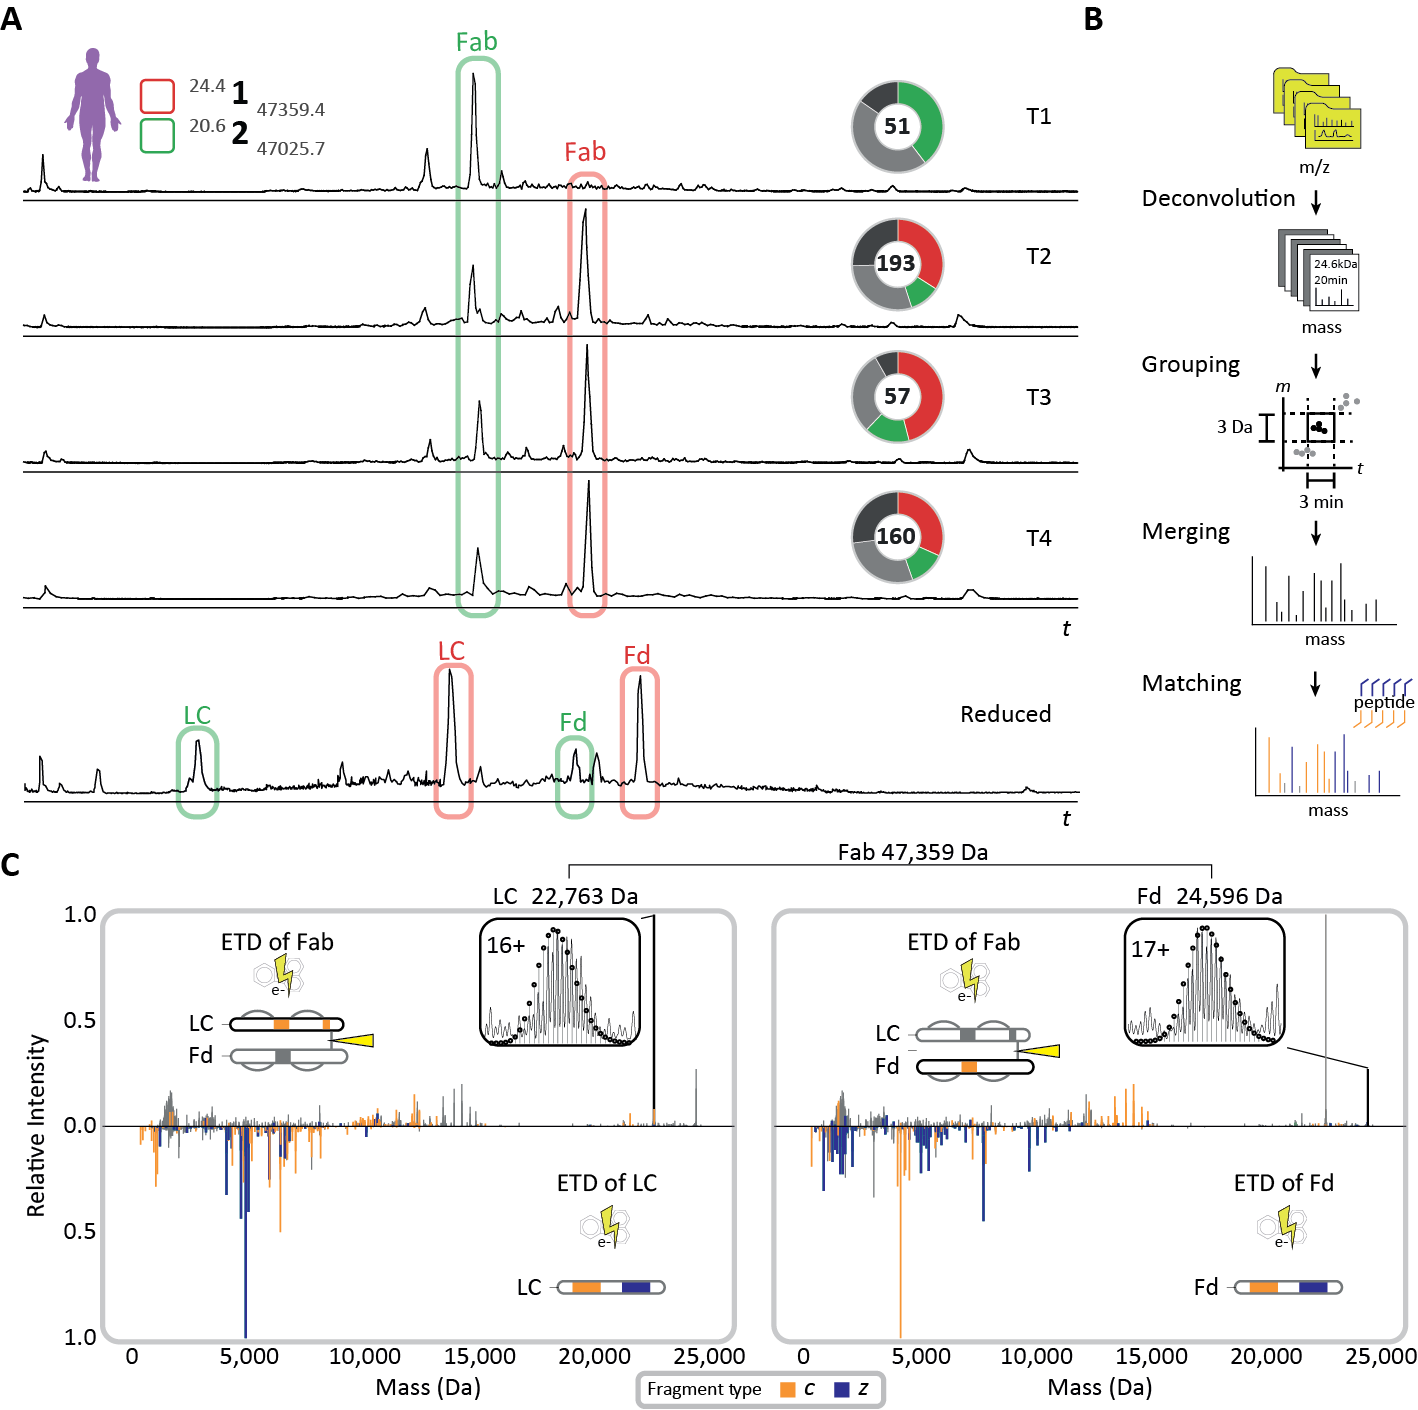
\includegraphics[]{Chapter.3/Figures/f3.png}
  \caption{
    \textbf{Middle-down sequence characterization of the Fab clone \textsuperscript{24.4} 1 \textsubscript{47,359.4} that becomes dominant in the repertoire after the onset of sepsis—under reducing and non-reducing conditions.}
    ~~a) Reversed-phase LC-MS base peak profiles of the Fab repertoire detected in samples T1-4 from donor F59 (top 4 profiles) reveal the dominance of a small number of clones, whereby especially clone \textsuperscript{24.4} 1 \textsubscript{47,359.4} becomes dominant in abundance after the onset of sepsis. The LC-MS chromatogram of the reduced and denatured Fab repertoire from donor F59 at T3 is depicted in the bottom panel. The light chains (LCs) and the N-terminal portions of the heavy chains (Fd) of the two dominant clones are annotated with corresponding colors and chain names. All species highlighted in red were subjected to middle-down LC-MS/MS using ETD. ~~b) Data processing workflow to prepare middle-down ETD-MS/MS spectra for fragment matching and sequence-tag detection (see Methods section for details). ~~c) Deconvoluted ETD-MS/MS spectra of the intact Fab (top spectra) and reduced LC and Fd fragments thereof (mirrored spectra) with the c/z-fragment ions annotated for the LC (left) and Fd (right). The isotopic envelopes of the most abundant charge states of the LC and Fd fragments released from the Fab upon ETD are depicted in the insets with theoretical isotope distributions of the corresponding chain sequences overlaid as black circles. Masses of the LC and Fd fragments and the cumulative mass of the Fab are indicated above the spectra. See also \textbf{\autoref{fig:figs3.6}} for more detail on the fragment ions identified in these middle-down MS spectra.
  }
  \label{fig:fig3.3}
\end{figure*}

Following fractionation and selection of the \textsuperscript{24.4} 1 \textsubscript{47,359.4} clone, we subjected this Fab to mass-spectrometry-based \emph{de novo} sequencing, combining data from middle-down and bottom-up proteomics (\textbf{\autoref{fig:fig3.1}b}). The \emph{de novo} sequence information from both approaches was used to first select several closely matching light- and heavy-chain templates from the publicly available IMGT database of IgG germline sequences (\textbf{\autoref{fig:figs3.5}; \autoref{tab:tabdummy3.3} and \autoref{tab:tabdummy3.4}}). Subsequently, the bottom-up and middle-down sequencing data and the measured intact accurate masses of the Fab, light chain, and Fd were used to refine the selected template sequences and ultimately determine the mature sequence present in the donor, revealing discrepancies between the germline and mature sequences.
In the protein-centric approach, we performed electron transfer dissociation (ETD) on the intact Fab, as well as the light chain and Fd separately, obtained by reduction of the Fab molecule (\textbf{\autoref{fig:fig3.3}a}, bottom trace). Several fragmentation scans obtained for the intact Fab, the separated light chain, and Fd were grouped and combined based on their unique precursor mass and retention time (\textbf{\autoref{fig:fig3.3}b}). The ETD mass spectra of the intact Fab yielded accurate masses of the light chain and Fd by cleavage of the interchain disulfide bond, thus providing direct information about the light-chain-heavy-chain pairing (\textbf{\autoref{fig:fig3.3}c}, top spectra). In addition, these ETD spectra yielded extended sequence tags, covering informative parts of the CDR3 and framework (FR) 4 regions of both Fab chains, in a similar manner as previously reported by performing ETD or ECD of intact IgG molecules \cite{boer2020selectivity, fornelli2017top-down, shaw2020direct}. Complementary, ETD spectra of the separated Fab chains yielded partial sequence information for the FR1, CDR1, FR2, CDR2, and the constant region of the selected clone (\textbf{\autoref{fig:fig3.3}c}, bottom spectra and \textbf{\autoref{fig:figs3.6}}). Although our middle-down MS data provided valuable information about the clone of interest, they did not fully cover the sequence, primarily due to incomplete fragment formation and ambiguous sequence information obtained from the larger fragments.
To further extend our sequencing attempt, we subjected the fraction containing the targeted IgG1 clone to enzymatic digestion, using in parallel four proteases: trypsin, chymotrypsin, thermolysin, and pepsin. The resulting peptides were analyzed by a bottom-up approach, using \emph{de novo} sequencing algorithms for sequence annotation \cite{peng2021mass}. Although fractionated and enriched for the desired \textsuperscript{24.4} 1 \textsubscript{47,359.4} clone, the bottom-up MS data also contained numerous peptides originating from co-isolated plasma clones (\textbf{\autoref{fig:figs3.7}}), which made it impossible to determine the correct sequence by solely using the bottom-up MS data. Nevertheless, by iteratively extending the sequence information from the middle-down MS approach with the \emph{de novo} peptides from the bottom-up MS approach, we ultimately were able to extract the most likely germline precursor of the targeted clone and, notably, its mature sequence by implementing various single-amino-acid mutations not present in the IMGT database (\textbf{\autoref{fig:fig3.4}}).
\begin{figure*}[!hptb]
  \center
  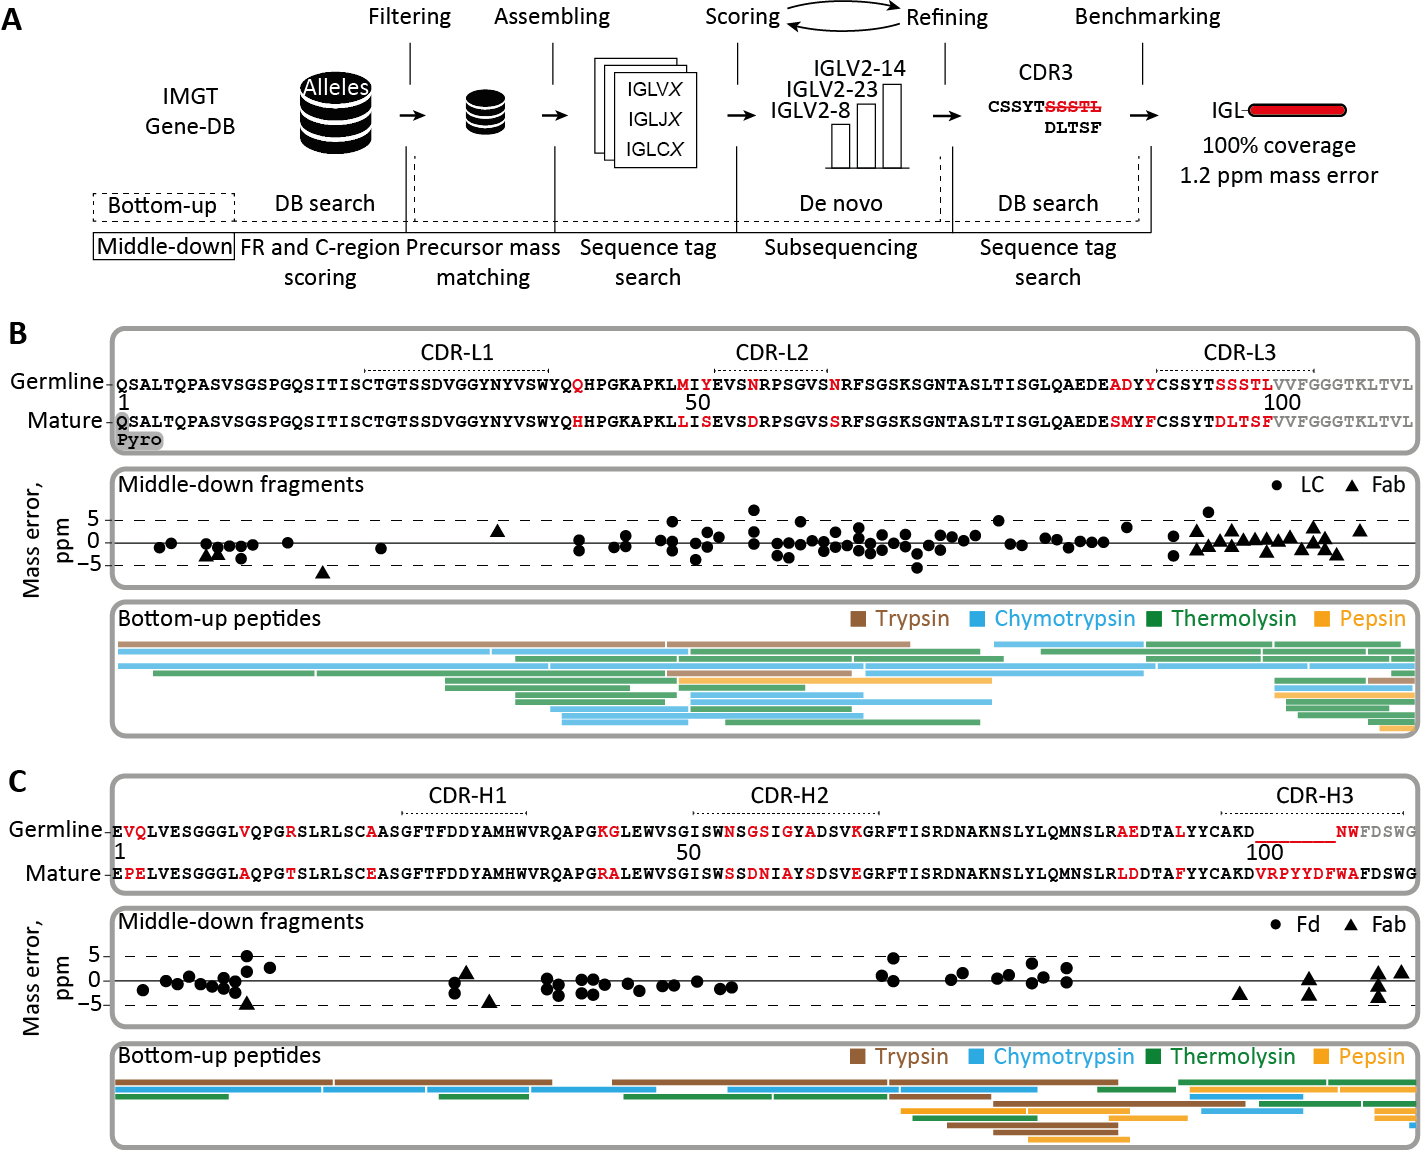
\includegraphics[]{Chapter.3/Figures/f4.png}
  \caption{
    \textbf{Integrative \emph{de novo} sequencing of the Fab clone \textsuperscript{24.4} 1 \textsubscript{47,359.4} from donor F59 combining middle-down and bottom-up MS data.} ~~a) Data analysis pipeline displaying the key steps in the \emph{de novo} sequencing, namely, filtering of the germline database of light- and heavy-chain sequences, assembling of selected allelic variants with mass constraints, scoring of the assembled sequences by using middle-down MS data, iterative refining of the best scoring templates by using peptides in bottom-up MS, and benchmarking of the optimized mature sequences using data from both middle-down and bottom-up MS analysis. ~~b) Alignment of the best matching germline IGLV amino acid sequence from the IMGT database (IGLV2-14$\star$01) with the mature sequence that was determined for the light chain of the dominant clone (top box), the fragments from middle-down MS (middle box), and the peptides from bottom-up MS. ~~c) Alignment of the best matching germline IGHV amino acid sequence from the IMGT database (IGHV3-9$\star$01) with the mature sequence that was determined for the Fd of donor F59’s clone \textsuperscript{24.4} 1 \textsubscript{47,359.4} (top box), the fragments from middle-down MS (middle box), and the peptides from bottom-up MS. CDR regions in top panels of ~~b) and ~~c) were annotated with reference to the closest matching IMGT sequence. Amino acids that were determined to be different in the mature \textsuperscript{24.4} 1 \textsubscript{47,359.4} sequence are highlighted in red.
  }
  \label{fig:fig3.4}
\end{figure*}

In more detail, by using the IMGT database of germline sequences as input, the cumulative MS evidence revealed that the analyzed IgG1 Fab carried a lambda light chain. This light chain originated from a combination of the immunoglobulin lambda (IGL) variable (V) 2-14$\star$01 (IMGT/LIGM-DB: Z73664), IGL joining (J) 2$\star$01 (IMGT/LIGM-DB: M15641), and IGL constant (C) 2$\star$01 (IMGT/LIGM-DB: J00253) alleles. For the heavy-chain Fd portion, we determined that it was constructed from the immunoglobulin heavy (IGH) V3-9$\star$01 (IMGT/LIGM-DB: M99651), IGHJ5$\star$01 (IMGT/LIGM-DB: J00256), and IGHG1$\star$03 (IMGT/LIGM-DB: Y14737) alleles and a diversity (D)-region, which substantially deviated from any reported germline D-region. Although initial identification resulted in just a partial sequence coverage, we could fill the gaps in the germline sequences using sequence tags from the middle-down MS and the \emph{de novo} peptides from the bottom-up MS (\textbf{\autoref{fig:figs3.8} and \autoref{fig:figs3.9}}). Eventually, our approach resulted in a complete and exact precursor mass match for the light and heavy chains, 100\% sequence coverage in bottom-up MS, and near-complete annotation of all available fragments in the middle-down MS data. In this process, numerous mutations had to be incorporated when comparing our data with the germline template sequences (\textbf{\autoref{fig:fig3.4}b and c}, in red letters), revealing somatic hypermutation (SHM) of around 13\% and 16\% for the V gene of the light chain and the heavy chain, respectively. The level of confidence in each identified mutation site is based on several criteria, including support of a mutation by consecutive mass peaks in the middle-down MS retrieved sequence tags, the peptide scores and coverage depth in the bottom-up MS data as well as the frequency of amino acid occurrence at a given position in a pool of experimental and the germline IgG1 sequences (\textbf{Data \ref{tab:tabdummy3.5}}; \textbf{\autoref{fig:figs3.10}}). Together this provides proof of concept that it is possible to \emph{de novo} sequence IgG1s present in plasma.
The definitive sequence assignment benefited largely from gathering multiple pieces of experimental evidence, notably (1) the accurate mass of the Fab, (2) the highly accurate masses of the two individual chains comprising the Fab, (3) the \emph{de novo} identified amino acid sequence reads, retrieved from the middle-down fragmentation of intact chains and intact Fab molecule, and (4) the \emph{de novo} identified amino acid reads from the—multiple proteases-based—peptide-centric bottom-up approach.

\subsection{Validation of the \emph{de novo} sequencing-derived sequence}
To validate the accuracy of the full \emph{de novo} sequence of the \textsuperscript{24.4} 1 \textsubscript{47,359.4} clone from donor F59, we generated a synthetic recombinant IgG1 clone based on the experimentally determined sequence. We used exactly the same procedures to sequence the recombinant mAb as applied to the plasma-obtained clone, including all the peptide- and protein-centric approaches. Since CDRs are the most critical and hypervariable regions of the antibody, we set out to find peptides in the two datasets covering these regions, so that we could directly compare their fragmentation spectra. A direct comparison of tandem MS spectra of the CDR-spanning peptides from the donor clone and the recombinant mAb are presented in \textbf{\autoref{fig:fig3.5}a and b}, covering parts of the light chain and Fd portion, respectively. Above the graphs, the \emph{de-novo}-obtained sequence is shown with the annotated CDRs, whereby the purple lines indicate the selected peptides. In each panel, the MS/MS spectra obtained from peptides derived from the plasma clone of donor F59 and the recombinant mAb are shown, with the donor spectrum on top and the recombinant mAb spectrum mirrored below. Through visual comparison and as evidenced by the high correlation scores ranging between 0.91 and 0.98, the spectra obtained for peptides originating from the recombinant clone were highly similar to the MS/MS spectra from the peptides derived from the plasma clone \textsuperscript{24.4} 1 \textsubscript{47,359.4}. The observed high similarity was not restricted to the \emph{m/z} positions but was found to be also reflected into fragment ion intensities, which are quite sequence specific, thus presenting an additional layer of confidence.
\begin{figure*}[!hptb]
  \center
  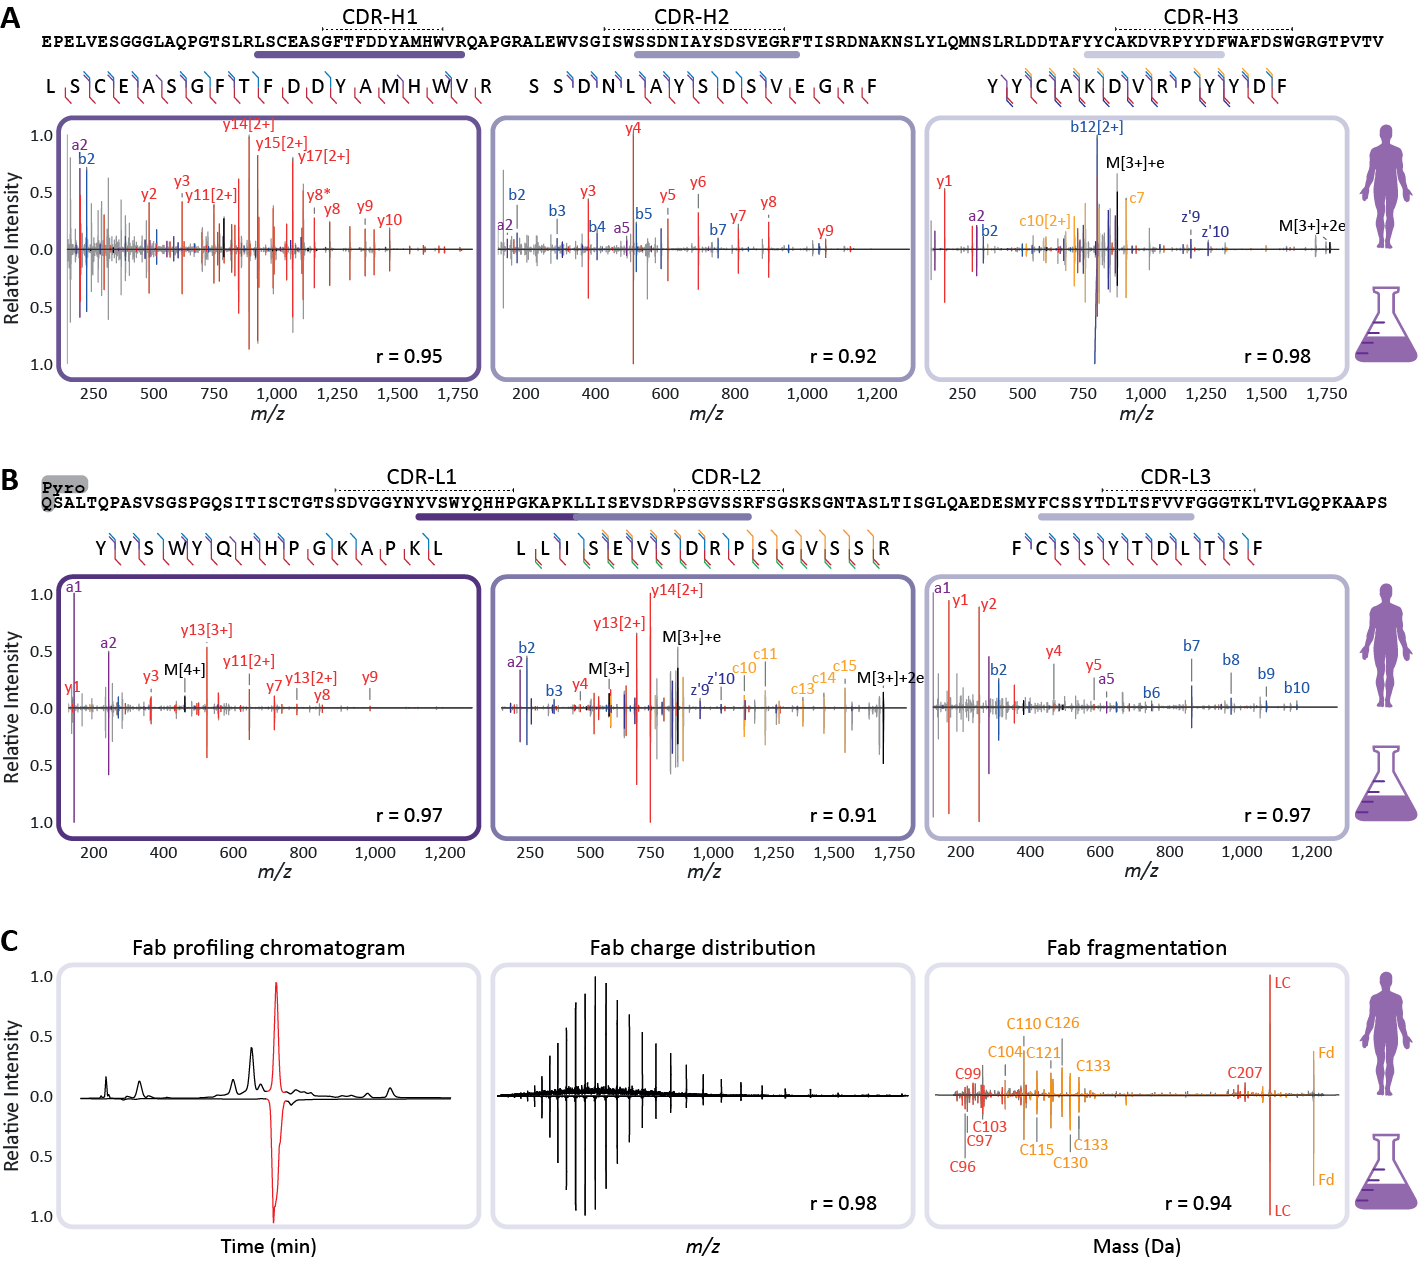
\includegraphics[]{Chapter.3/Figures/f5.png}
  \caption{
    \textbf{Comparison of sequencing data for clone \textsuperscript{24.4} 1 \textsubscript{47,359.4} of the donor F59, and the corresponding recombinant mAb validates the correctness of the \emph{de novo} sequencing approach.} ~~a) Peptide fragmentation spectra of CDR-spanning peptides from the HC of the dominant \textsuperscript{24.4} 1 \textsubscript{47,359.4} clone with, mirrored to each other, annotated spectra from the donor (top) and the recombinant IgG1 (bottom). ~~b) Peptide fragmentation spectra of CDR-spanning peptides from the LC of the dominant \textsuperscript{24.4} 1 \textsubscript{47,359.4} clone with, mirrored to each other, annotated spectra from the donor (top) and the recombinant IgG1 (bottom). Spectra in ~~a) and ~~b) are annotated with \emph{a}-ions in purple, \emph{b}-ions in blue, \emph{y}-ions in red, \emph{c}-ions in orange, and \emph{z}-ions in dark blue. Corresponding fragmentation maps are displayed above each spectral pair. ~~c) Comparison of the middle-down LC-MS/MS analysis of the \textsuperscript{24.4} 1 \textsubscript{47,359.4} clone and the recombinant IgG1. Shown are the base peak chromatograms (left panel), the charge-state distributions detected in MS1 of the Fab (middle panel), and the deconvoluted ETD fragmentation spectra for the donor (top) and recombinant (bottom) IgG (right panel). The Pearson correlation coefficients (r) calculated for all demonstrated spectral pairs in ~~a) , ~~b) , and ~~c) are indicated at the bottom of each spectrum.
  }
  \label{fig:fig3.5}
\end{figure*}


Such a direct comparison of spectral features was extended to the middle-down analysis, used for obtaining sequence tags of the intact Fab (\textbf{\autoref{fig:fig3.5}c}). The intact recombinant Fab displayed a nearly identical retention time profile when compared with the plasma clone \textsuperscript{24.4} 1 \textsubscript{47,359.4} Fab (\textbf{\autoref{fig:fig3.5}c}, left panel). Furthermore, both clone \textsuperscript{24.4} 1 \textsubscript{47,359.4} and the recombinant mAb emerged with nearly identical charge distributions (\textbf{\autoref{fig:fig3.5}c}, middle panel), whereby the slight differences in the distribution are likely due to the underlying background of co-eluting Fabs in the plasma-derived sample. Nevertheless, the masses detected for the two Fabs were identical, i.e., within a 20-ppm mass error. Moreover, when the intact Fabs were subjected to ETD, alike fragment masses and retention times for both the light chain and Fd were observed, comparing the recombinant mAb with the plasma-derived clone. Finally, the generated lower mass fragment ions used for sequence-tag generation were also very similar (\textbf{\autoref{fig:fig3.5}c}, right panel). Likewise, the in-solution reduction of the Fabs revealed that there were no mass differences between the donor clone and recombinant mAb (light chain and Fd mass within 10 ppm).
Based on all these data, we can conclusively state that the sequence of the plasma-derived clone \textsuperscript{24.4} 1 \textsubscript{47,359.4} is identical to that of the recombinant mAb, with practically identical data observed at every step of our integrative \emph{de novo} sequencing approach. This not only validates the accuracy of the IgG1 sequence that we obtained for clone \textsuperscript{24.4} 1 \textsubscript{47,359.4} but also reinforces that the methodology presented here can be used to derive the correct full sequences from individual clones even when they are in a background of other plasma (highly sequence-homologous) IgG1 clones. Although this whole analysis pipeline is still quite arduous, requiring manual validation throughout the process, we consider this proof of concept a major step forward and expect that further fine-tuning of the algorithms will enhance the throughput in the future.

\section{Discussion}
The human body can make billions of different antibodies, stemming from the versatile and complex recombination process, accompanied by additional somatic hypermutations, helping us to adapt to a life-long exposure to various pathogens. Here, we demonstrate that it is feasible to profile the IgG1 repertoire of individual donors qualitatively and quantitatively by LC-MS, following the capturing of IgGs from plasma and analyzing the generated IgG1 Fab fragments. From this technical advance, one of the key observations we make is that in all studied donors at all time points, only a limited number of IgG1 clones dominate an individual’s repertoire. In all donors, the 30 most abundant clones make up two-thirds of all detected circulating IgG1 molecules; in one donor just two clones contributed $\sim$50\% to the detected serum population of IgG1 molecules. The IgG1 clonal profiles are found to be unique for each donor. Within a donor, the profiles are highly similar across time, but they also adapt to physiological changes (e.g., sepsis). The mass-spectrometry-based approach requires only minute amounts of plasma ($\sim$10 μL) and does not involve labor-intensive enrichment protocols. We further show that specific IgG clones can be extracted from the plasma and analyzed in depth, ultimately leading to the mass-spectrometry-based \emph{de novo} sequencing of the whole Fab molecule. Therefore, one of the holy grails in proteomics, \emph{de novo} sequencing of antibodies directly extracted from plasma, seems to be within reach.
The ultimate mature sequence of \textsuperscript{24.4} 1 \textsubscript{47,359.4} clone we sequenced here revealed that around 13\% and 16\% of the amino acids of the V-regions of light and heavy chains were different when compared with the closest germline sequence match within the IMGT database. This number of mutations is higher than the reported average (7\%) for IgG1 heavy-chain variable regions, as determined from RNA sequences \cite{kitaura2017different}. This suggests that DNA/RNA templates of the IgG sequences can be helpful, but for obtaining the correct sequence of the circulating clone, analyzing sequences at the level of the proteins will be essential.
The ability to \emph{de novo} sequence the whole Fab molecule is the result of combining, iteratively, middle-down and bottom-up proteomics data. An alternative strategy employed is to combine bottom-up proteomics data with BCR sequences using RNA sequencing of one donor to generate a database to match this donor’s Ig bottom-up proteomics data against \cite{lee2016molecular-level}. Although also very powerful, a recent application of this approach highlighted further the relevance of antibody sequencing at the level of proteins, when it was shown that for the six potent anti-HIV1 antibodies found by antigen-specific single-B-cell sequencing, only three could also be detected in circulation as IgG protein products \cite{williams2017potent}. All these issues highlight the necessity of direct analysis of the serum Ig repertoire at the protein level, as we now demonstrated here to be feasible.
Longitudinal quantitative clonal profiling, as presented here, opens a myriad of future prospects, both fundamental and applied. It allows to advance our understanding of B cell biology and antibody dynamics. Historically, general observations have been made about antibody half-lives using a single dose of labeled antibodies \cite{morell1970metabolic} or by determining the restoration of normal IgG levels following high-dose administrations of intravenous IgG \cite{melamed2018pharmacokinetics}. Through the method presented here, we can monitor the longitudinal abundance of each single clone in the circulation and monitor how it responds to changes in the donor’s physiology. Given the approximately 20-day IgG antibody half-life, it is expected that in the time span studied here (10–63 days), a decay in the concentration of clones would be detected. Indeed, we do observe several diminishing clones as depicted in \textbf{\autoref{fig:fig3.2} and \autoref{fig:figs3.4}}. However, other patterns are also observed, indicative of continuous production of the clone, even over a time window of two months. This is in line with previous reports on the presence of and production of antibodies by long-lived plasma cells, both in mice and humans \cite{bernasconi2002maintenance, manz1997lifetime, slifka1998humoral}. In addition, persistence of autoreactivity has been reported before \cite{tebani2020integration}, as well as persistence of antibody clonotypes detected by CDR-H3 proteomics \cite{lee2019persistent}. From our data, we cannot derive information regarding (auto)reactivity, but the data do suggest that long-term stability is not exclusive to autoantibodies and is instead a common phenomenon.
In summary, the \emph{de novo} sequencing at the protein level of IgG clones circulating in plasma is shown here to be feasible. We demonstrate the synergistic power of combining iteratively peptide- and protein-centric-based sequencing, which is capable of not only identifying the distinct alleles from which a clone originates but also its entire mature sequence. The work presented here is still quite a laborious proof of concept. Our aim for the future is quantitative monitoring and mass-spectrometry-based sequencing of multiple serum immunoglobulins directly at the protein level, i.e., as they appear in circulation and function in the human immune response.

\subsection{Experimental model and subject details}

\subsubsection{Human subjects}
We obtained longitudinal plasma samples from the Molecular Diagnosis and Risk Stratification of Sepsis (MARS) biorepository (ClinicalTrials.gov identifier NCT01905033), for which subjects had been included in the mixed ICU of a tertiary teaching hospital in the Netherlands (University Medical Centre Utrecht, Utrecht) since January 2011. Donors were enrolled via an opt-out consent method approved by the institutional review board of the UMC Utrecht (IRB no. 10-1056C). Daily leftover EDTA plasma (obtained from blood drawn during routine care) was stored at -80 °C until use.
For the current study, we included eight patients with esophageal or gastroesophageal junction cancer who underwent an elective esophagectomy and gastric pull-through procedure and had subsequently developed an infectious complication (i.e., anastomotic leakage or pneumonia). These patients were all admitted to the Intensive Care Unit on two occasions. The first admission concerned routine observation after elective resection followed by an uncomplicated ICU stay of fewer than 2 days. All patients were subsequently readmitted to the ICU due to sepsis. For all episodes of sepsis, microbiological cultures were obtained either before or during ICU readmission, and clinical infection was adjudicated highly plausible according to pre-defined criteria \cite{klouwenberg2013interobserver}. Furthermore, all infectious episodes met SIRS criteria and had a Sequential Organ Failure Assessment (SOFA) score ≥ 2, thus fulfilling current Sepsis-3 definitions \cite{singer2016third}. All patients were ultimately discharged from ICU in a clinically stable condition. We analyzed plasma samples obtained at four well-defined time points: within 24 hours of surgery when no signs of sepsis were present (sample T1), on two consecutive days after onset of sepsis (samples T2 and T3), and upon ICU discharge following resolution of sepsis (sample T4). Patient characteristics are summarized in \textbf{Data \ref{tab:tabdummy3.2}}. All patients had been treated with neoadjuvant chemoradiotherapy prior to surgery. None of the patients received treatment with immunoglobulins or monoclonal antibodies either prior to or during ICU admission.
In addition, longitudinal EDTA plasma samples from two healthy Caucasian donors were purchased from Precision Med (Solana Beach, CA, US). The samples were part of the ‘Normal Control Collections’, protocol number 7005-8200. These donors were selected having similar characteristics as the sepsis donors regarding age and gender.

\subsection{Method details}

\subsubsection{Plasma IgG purification and Fab generation}
The IgG purification and generation of Fabs was adapted from an earlier published protocol \cite{bondt2014immunoglobulin}. The FcXL affinity matrix used in the workflow, which binds to the CH3 domain of the IgG constant region, has recently been shown not to provide a bias regarding analysis of the Fc glycosylation residing in the CH2 domain \cite{amezmartín2021serum}. Mobicol spin filters were assembled according to the manufacturer’s instructions and placed in 2 mL Eppendorf tubes. Then 20 μL FcXL affinity matrix slurry was added to the spin filter, followed by three washing steps with 150 μL PBS, in which the liquid was removed by centrifugation for 1 min at 1000 × g. Two additional washing steps with 150 μL were performed. After washing, the 2 mL tube was replaced by a 1.5 mL tube. The affinity matrix was resuspended in 150 μL PBS, and 10 μL plasma was added. Furthermore, 1 μL of a solution containing two known mAbs at 200 μg/mL each was added, corresponding to 20 μg/mL when calculated to the plasma concentration. The samples were then incubated, under shaking conditions for one hour at room temperature. After the incubation, the flow-through was collected, and the affinity matrix with bound IgGs was washed four times with 150 μL PBS. Finally, 50 μL PBS containing 100 U of the IgdE (FabALACTICA; Genovis AB, Lund, Sweden) protease was added before incubating on a thermal shaker at 37 °C for >16 hours. After the incubation, 10 μL of Ni-NTA beads were added to bind and remove the His-tagged protease, whereafter the samples were incubated for an additional 30 minutes. The flow through after centrifugation contained the Fab fragments generated from IgG1.

\subsubsection{Method optimization and validation using a mixture of recombinant mAbs}
In an array of experiments, we optimized and validated the robustness and accuracy of our IgG1 capturing approach, the generation of the Fab fragments and the analysis of the Fab LC-MS profiles. Therefore, we prepared a mixture of six IgG1 monoclonal antibodies, including the two spiked into every plasma sample subsequently analyzed. For the method optimization the 6 recombinant mAbs were added to the plasma of a single donor in different quantities: 4,000, 800, 200, 20, 2, or 0.5 ng per mAb. The mAbs used were trastuzumab (Roche, Penzberg, Germany), alemtuzumab (Genmab, Utrecht, The Netherlands), the Fab glycosylated cetuximab, rituximab, bevacizumab, and infliximab (Evidentic, Berlin, Germany). Fab sequences and theoretical masses of these mAbs, including the most abundant cetuximab glycoforms, are shown in \textbf{Data \ref{tab:tabdummy3.1}}. All these samples were injected once, except for the 200 ng sample which was injected three times to provide additional injection replicates.

\subsubsection{LC-MS(/MS)}
Reversed-phase liquid chromatography was performed by using a Thermo Scientific Vanquish Flex UHPLC instrument, equipped with a 1 mm x 150 mm MAbPac RP analytical column, directly coupled to an Orbitrap Fusion Lumos Tribrid (Thermo Scientific, San Jose, CA, USA) or Q Exactive HF-X mass spectrometer (Thermo Fisher Scientific, Bremen, Germany). The column preheater, as well as the analytical column chamber, were heated to 80 °C during chromatographic separation. Both samples, either containing intact Fabs or separate Fab chains, were separated over 62 min at a 150 μL/min flow rate. Gradient elution was achieved by using two mobile phases A (0.1\% HCOOH in Milli-Q) and B (0.1\% HCOOH in CH3CN) and ramping up B from 10 to 25\% over one minute, from 25 to 40\% over 55 min, and from 40 to 95\% over one minute. MS data were collected with the instrument operating in Intact Protein and Low Pressure mode. Spray voltage was set at 3.3 kV, capillary temperature 350 °C, probe heater temperature 100 °C, sheath gas flow 35, auxiliary gas flow 10, and source-induced dissociation was set at 15 V. The electrospray voltage was applied after 2 min to prevent the salts in the sample from entering the MS. Intact Fabs were recorded with a resolution setting of 7,500 (@ \emph{m/z} 200) in MS1, which allows for better detection of charge distributions of the large proteins (> 30 kDa) \cite{waterbeemd2018dissecting}. Separate Fab chains were analyzed with a resolution setting of 120,000 (@ \emph{m/z} 200) in MS1, which allows for more accurate mass detection of smaller proteins (< 30 kDa). MS1 scans were acquired in a range of 500-3,000 Th with the 250\% AGC target and a maximum injection time set to either 50 ms for the 7,500 resolution or 250 ms for the 120,000 resolution. In MS1, 2 μscans were recorded for the 7,500 resolution and 5 μscans for the 120,000 resolution per scan. Data-dependent mode was defined by the number of scans: single scan for intact Fabs and two scans for separate Fab chains. In both cases, MS/MS scans were acquired with a resolution of 120,000, a maximum injection time of 500 ms, a 1,000\% AGC target, and 5 μscans averaged and recorded per scan. The ions of interest were mass-selected by quadrupole in a 4 Th isolation window and accumulated to the AGC target prior to fragmentation. The electron-transfer dissociation (ETD) was performed using the following settings: 16 ms reaction time, a maximum injection time of 200 ms, and the AGC target of 1e6 for the ETD reagent. For the data-dependent MS/MS acquisition strategy, the intensity threshold was set to 2e5 of minimum precursor intensity. MS/MS scans were recorded in the range of \emph{m/z} = 350-5,000 Th using high mass range quadrupole isolation.

\subsubsection{Clonal profiling data analysis}
Masses were retrieved from the generated RAW files using BioPharmaFinder 3.2 (Thermo Scientific). Deconvolution was performed using the ReSpect algorithm between 5 and 57 min using 0.1 min sliding window with 50\% offset and a merge tolerance of 50 ppm, with noise rejection set at 95\%. The output mass range was set at 10,000 to 100,000 with a target mass of 48,000 and mass tolerance of 30 ppm. Charge states between 10 and 60 were included, and the Intact Protein peak model was selected. Further data analysis was performed using Python 3.8.10 (with libraries: Pandas 1.2.4 \cite{mckinney2010data}, Numpy 1.20.2 \cite{walt2011numpy}, Scipy 1.6.2 \cite{virtanen2020scipy}, Matplotlib 3.3.4 \cite{hunter2007matplotlib:} and Seaborn 0.11.1). Masses of the BioPharmaFinder identifications (components) were recalculated using an intensity weighted mean considering only the most intense peaks comprising 90\% of the total intensity. Furthermore, using the data of two spiked-in mAbs (trastuzumab and alemtuzumab) a mass correction was applied based on the difference between the calculated and observed mAb masses, and similarly, a retention time alignment was applied to minimize deviation between runs.
Components between 45,000 and 53,000 kDa with the most intense charge state above \emph{m/z} 1,000 and score ≥40 were considered Fab portions of IgG clones. The clones were matched between runs using average linkage (unweighted pair group method with arithmetic mean UPGMA) L∞ distance hierarchical clustering. Flat clusters were formed based on a cophenetic distance constraint derived from the mass and retention time tolerance. These tolerances were defined as three times the standard deviation of the mAb standards, which were 1.4 Da and 0.8 min, respectively. Clones within a flat cluster were considered identical between runs.

\subsubsection{Peptide-centric (bottom-up) \emph{de novo} sequencing}
Clones of interest were captured through fraction collection using the same chromatography setup used for LC-MS profiling. Samples were dried under vacuum and resuspended in a 50 mM ammonium bicarbonate buffer. To boost signal intensity, the fractions were pooled across the time points. Samples were equally split for digestion with four proteases.
For digestion with trypsin, chymotrypsin and thermolysin, a sodium deoxycholate (SDC) buffer was added to a total volume of 80 μL, 200 mM Tris pH 8.5, 10 mM tris(2-carboxyethyl)phosphine (TCEP), 2\% (w/v) SDC final concentration. For pepsin digestion, a urea buffer was added to a total volume of 80 μL, 2M Urea, 10 mM TCEP. Samples were denatured for 10 min at 95 °C followed by reduction for 20 min at 37 °C. Next, iodoacetic acid was added to a final concentration of 40 mM and incubated in the dark for 45 min at room temperature for alkylation of free cysteines. Then for trypsin, chymotrypsin and thermolysin 50 mM ammonium bicarbonate buffer was added to a total volume of 100 μL. For pepsin 1 M HCl was added to a final concentration of 0.04 M. 0.1 μg of each protease was added and incubated for 4 hours at 37 °C. After digestion 2 μL HCOOH was added to precipitate the SDC. SDC was removed by centrifugation for 20 min at max speed (20,817 × ~~g) after which the supernatant was moved to a new tube.
Samples were desalted by Oasis HLB (Waters Corporation, Millford, MA, USA) following a 5-step protocol. 1) Sorbent was wetted using 2x 200 μL CH3CN, 2) followed by equilibration with 2x 200 μL water/10\% HCOOH. 3) The sample was loaded and 4) washed with 2x 200 μL water/10\% HCOOH. 5) Finally, the sample was eluted using 2x 50 μL water/50\% CH3CN /10\% HCOOH and dried down by vacuum centrifuge. Prior to MS analysis samples were reconstituted in 2\% HCOOH.

\paragraph{LC-MS/MS}
Data acquisition was performed on the Orbitrap Fusion Tribrid Mass Spectrometer (Thermo Scientific, San Jose, CA, USA) coupled to UHPLC 1290 system (Agilent Technologies, Santa Clara, CA, USA). Peptides were trapped (Dr. Maisch Reprosil C18, 3 μm, 2 cm × 100 μm) prior to separation (Agilent Poroshell EC-C18, 2.7 μm, 500 mm × 75 μm). Trapping was performed for 10 min in solvent A (0.1\% HCOOH in Milli-Q), and the gradient was as follows: 0 – 13\% solvent B (0.1\% HCOOH in 80\% CH3CN) over 5 min, 13 – 44\% solvent B over 65 min, 44 – 100\% solvent B over 4 min, and 100\% B for 4 min (flow was split to achieve the final flowrate of approximately 200 nL/min). Mass spectrometry data was collected in a data-dependent fashion with survey scans ranging from 350-2,000 Th (resolution of 60,000 @ \emph{m/z} 200), and up to 3 sec for precursor selection and fragmentation with either stepped higher-energy collisional dissociation (HCD) set to [25\%, 35\%, 50\%] or electron transfer dissociation (ETD), used with charge-normalized settings and supplemental activation of 27\%. The MS2 spectra were recorded at a resolution of 30,000 (@ \emph{m/z} 200). The AGC targets for both MS and MS2 scans were set to standard within a maximum injection time of 50 and 250 ms, respectively.

\paragraph{Data analysis}
Raw LC-MS/MS data were processed using PEAKS X software (Bioinformatics Solutions Inc., Waterloo, ON, Canada) for \emph{de novo} sequencing of peptides. The following parameters were used for \emph{de novo} sequencing: parent mass error tolerance – 12 ppm, fragment mass error tolerance – 0.02 Da, max number of variable PTMs per peptide – 3. Fixed modifications: Carboxymethyl; variable modifications: Oxidation (HW), Oxidation (M), Pyro-glu from E, Pyro-glu from Q, Carboxymethyl (KW, X@N-term), and Carbamylation. Resulting \emph{de novo} peptide tables were exported as.csv files and used for filtering of the IMGT database and determination of the mature \textsuperscript{24.4} 1 \textsubscript{47359.4} clone sequences.

\subsubsection{Protein-centric (middle-down) \emph{de novo} sequencing}
Fab samples were prepared without treatment as well as under denaturing and reducing conditions for analysis of intact Fab and separate Fab chains, respectively. The latter were denatured and reduced in 10 mM TCEP at 60 °C for 30 min prior to LC-MS/MS analysis. Approximately 2-5 μg of each sample was injected for a single middle-down LC-MS(/MS) experiment using the parameters described above.

\paragraph{Data analysis}
Full middle-down MS spectra were deconvoluted with either Xtract \cite{zabrouskov2005new} or ReSpect (Thermo Fisher Scientific, Bremen, Germany) for isotopically-resolved (separate Fab chains) or unresolved (intact Fabs) data, respectively. Middle-down LC-MS/MS data were charge-deconvoluted and deisotoped into singly-charged mass spectra using the ‘Parallel Xtract’ node and converted to mascot generic format (mgf) files in Thermo Proteome Discoverer (version 2.3.0.523; Thermo Fisher Scientific, Bremen, Germany). Deconvolution parameters were set as follows: ReSpect: precursor \emph{m/z} tolerance – 0.2 Th; relative abundance threshold – 0 \%; precursor mass range from 3 to 100 kDa; precursor mass tolerance of 30 ppm; charge states between 3 and 100. Xtract: signal/noise threshold of 3; \emph{m/z} range – 500-3,000 Th.
For the analysis of the final mature Fab chains of the most abundant clone in the plasma of patient F59, we used an integrative approach that utilizes bottom-up and middle-down data and the international ImMunoGeneTics information system (IMGT) database (\textbf{\autoref{fig:fig3.3}b}). First, the replicate middle-down MS/MS spectra were grouped per deconvoluted mass feature in the LC-MS-only runs by using a 3 Da mass window and a 3 min retention time window. The resulting grouped spectra were merged into a single spectrum, whereby peaks’ intensities were combined when they coincided within a 2 ppm window. The identity of the constant domain (C-) gene was determined by matching the fragments in these combined spectra to a database of all functional, open reading frame, and in-frame pseudogene alleles for C-genes retrieved from IMGT/Gene-DB \cite{lefranc1999imgt}. Next, bottom-up LC-MS/MS spectra of the fractionated \textsuperscript{24.4} 1 \textsubscript{47359.4} clone were screened against a database of all functional, open reading frame, and in-frame pseudogene alleles for the variable domain (V-) genes retrieved from the IMGT/Gene-DB \cite{lefranc1999imgt}, using local Smith-Waterman alignment with the BLOSUM62 matrix in which the common \emph{de novo} sequencing errors I/L, Q/E and N/D were modified to neutral substitutions \cite{smith1981identification}. From any gene regions with confident peptide matches (FDR < 1\%), we then took the FR1, 2 and 3 regions and subjected them to an in-house scoring algorithm to score their agreement with our middle-down data (\textbf{\autoref{fig:figs3.5}}). In short: the algorithm searches for peak patterns that would occur as a result of fragmentation of the provided sequence regions, disregarding preceding and succeeding parts of the initial sequence. Ranking the gene regions by a resulting composite score enabled us to select top-scoring templates as a starting point for our sequencing efforts as well as discard low-scoring regions from further analyses. The remaining gene regions were then used to in silico generate a database of germline light and heavy chains.
Then, using a custom implementation of the DirecTag algorithm \cite{tabb2008directag:}, all possible sequence tags were detected and annotated in the combined middle-down spectra. These sequence tags were used to search the filtered germline light and heavy IgG chains. For the best scoring germline sequences, consistent sequence tags with a length of more than 4 amino acids were searched against \emph{de novo} predicted peptides originating from the bottom-up peptide-centric MS data. In an iterative manner, the matching peptides were used to modify the best scoring selected germline sequences until the mass of the final sequence matched the precursor masses determined by middle-down MS (\textbf{\autoref{fig:figs3.8} and \autoref{fig:figs3.9}}). In more detail, the gaps between the consecutive sequence tags extracted from the middle-down MS data were first filled with amino acids from the best matching germline sequence. Then, the filled gaps were compared to the highest scoring peptides retrieved from the bottom-up MS data, aligned to the region of interest using Clustal Omega algorithm. When aligned peptides showed discrepancies from the germline sequence the amino acid residues in the gaps were altered and the theoretical mass of the gap was compared to the experimental mass, defined by the mass difference between consecutive sequence tags. Finally, the modified sequences were rescored by spectral alignment, sequence-tag detection, and a bottom-up database search, providing the final mature Fab sequences. The final predicted sequences – and more specifically the identified mutations when compared to the most closely related gene regions – were additionally compared to the frequency of amino acid occurrence at their specific positions (as numbered by IMGT) in both the AbYsis database \cite{swindells2017abysis:} and the recombined full IMGT database \cite{lefranc1999imgt}. This screening yielded an estimate of how likely the mutations were to occur. While some of the predictions are rather rare, none of them are impossible as reported by AbYsis (\textbf{Data \ref{tab:tabdummy3.5}}).

\subsection{Quantification and statistical analysis}
For quantification of LC-MS profiling data, the intensity values of the two mAb standards (trastuzumab and alemtuzumab) were averaged in each run and set to 20 μg/mL. The intensity values of all other detected Fabs were normalized to these values in order to determine the concentration of each individual clone. For the quantification of mAbs in the validation experiment, a slightly different normalization was used. The intensity values of the detected mAbs in all runs were normalized to the intensity values of trastuzumab and alemtuzumab as measured in the first 200 ng replicate.
Statistical values in figures depicted as lower-case letter r indicate Pearson correlation coefficients. Distances between samples as shown in \textbf{\autoref{fig:fig3.2}b} were determined by distance correlation. Linear regression for validation of quantification \textbf{\autoref{fig:figs3.1}b} was determined by ordinary least squares regression with the coefficient of determination given as uncentered R\textsuperscript{2}. The error-bars in the figure represent the standard error of the mean (SEM).

\section{Acknowledgments}
This research received funding through the Netherlands Organization for Scientific Research (NWO) through the ENPPS.LIFT.019.001 project (A.J.R.H. and J.F.G.), the NACTAR project 16442 (A.J.R.H. and M.A.d.B.), Gravitation Subgrant 00022 from the Institute for Chemical Immunology (A.B., D.M.H.v.R., W.P., D.S., and J.S.), and the Spinoza award SPI.2017.028 to A.J.R.H. This project received additional funding from the European Union’s Horizon 2020 research and innovation program under the grant agreement 686547 (EPIC-XS) for A.J.R.H. We kindly acknowledge the teams of Janine Schuurman, Frank Beurskens, and Boris Bleijlevens (Genmab, Utrecht, NL) for continuous support over the years, stimulating discussions, financial co-support for A.B. and S.T., and the generation of the recombinant clone based on the sequence of the plasma clone \textsuperscript{24.4} 1 \textsubscript{47,359.4}. We thank Dietmar Reusch and Markus Haberger (Roche, Penzberg) for the kind donation of trastuzumab.

\subsection{Author contributions}
A.J.R.H. conceived the idea for this study. A.B., S.T., and A.J.R.H. designed the research, planned the experiments, and supervised the project. A.B., M.H., M.A.d.B., and D.M.H.v.R. performed the IgG capture from serum and subsequent generation of Fabs, subsequently analyzed by intact LC-MS. M.H. developed the repertoire profiling bioinformatics workflow. S.T. performed the middle-down MS/MS analysis of the clones and in collaboration with S.C.d.G generated the bioinformatics workflow to analyze the data. W.P., M.H., D.S., and J.S. performed all bottom-up proteomics experiments and subsequent data analysis. S.T. and S.C.d.G performed the de novo sequencing through the  iterative integration of middle-down and bottom-up proteomics data. J.-F.G. contributed to study design and data analysis. M.V., M.J.M.B., and O.L.C. provided the MARS cohort samples and selected the patient population used in this study. A.B., M.H., S.T., and A.J.R.H. wrote the original draft, which was read, improved, and approved by all co-authors.

\subsection{Declaration of interests}
The authors declare no competing interests.
\clearpage
\begin{subappendices}

  \section{Supplementary material}
  \beginsupplement
  Supplementary Table 1-5 and Supplementary Data 1-3 can be found online at:\\
  \emph{https://doi.org/10.1016/j.cels.2021.08.008}\\

  \vspace{24cm}

  \refstepcounter{table}
  \label{data:datadummy3.1}
  \refstepcounter{table}
  \label{data:datadummy3.2}
  \refstepcounter{table}
  \label{data:datadummy3.3}
  \addtocounter{table}{-3}
  \refstepcounter{table}
  \label{tab:tabdummy3.1}
  \refstepcounter{table}
  \label{tab:tabdummy3.2}
  \refstepcounter{table}
  \label{tab:tabdummy3.3}
  \refstepcounter{table}
  \label{tab:tabdummy3.4}
  \refstepcounter{table}
  \label{tab:tabdummy3.5}
  \addtocounter{table}{-6}

  \begin{figure*}[!h]
    \center
    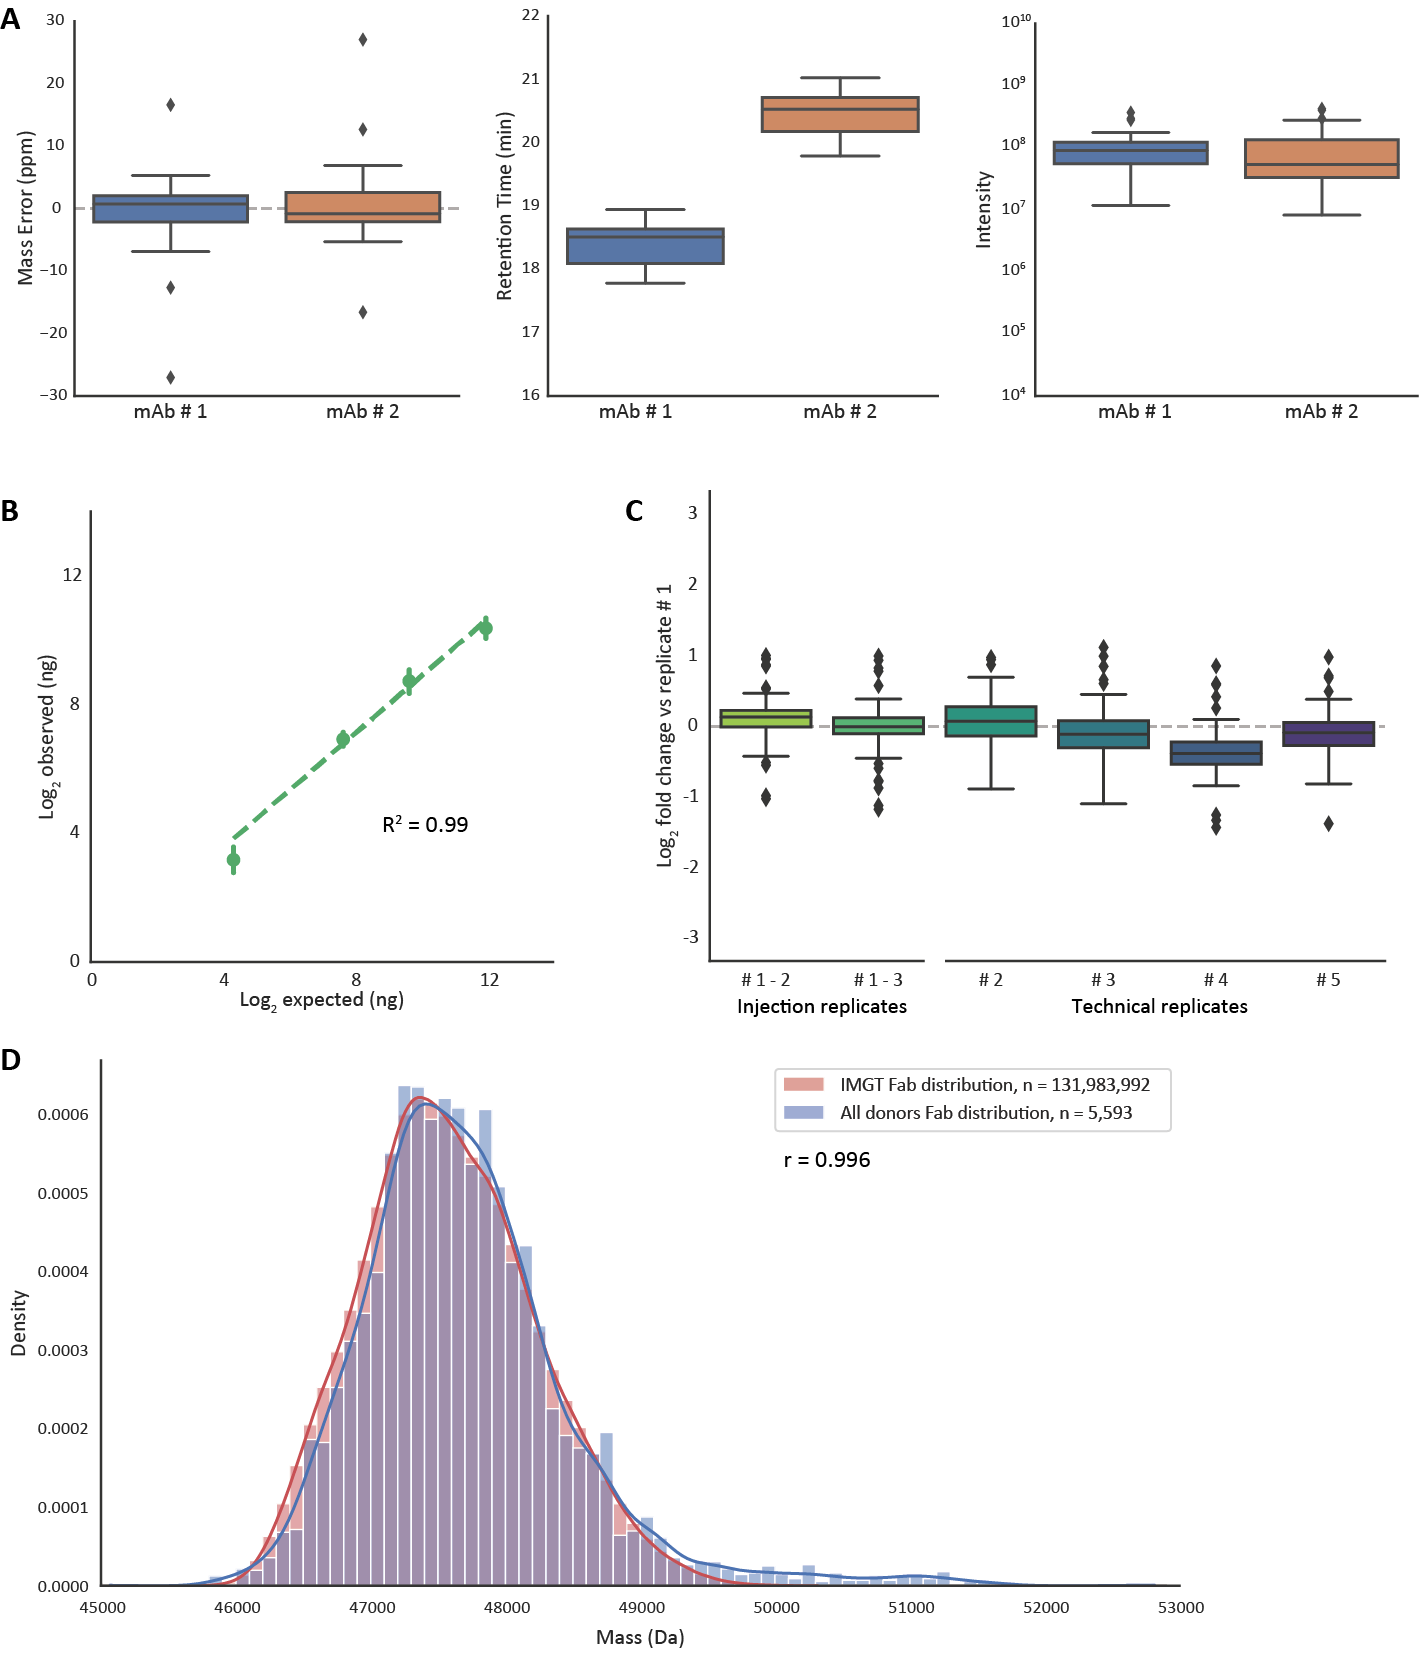
\includegraphics[]{Chapter.3/Figures/fs1.png}
    \captionsetup{singlelinecheck = false, format= hang}
    \caption{
      Figure legend on next page.
    }
    \label{fig:figs3.1}
  \end{figure*}
  \addtocounter{figure}{-1}
  \begin{figure*}[t!]
    \caption{
      \textbf{Performance evaluation of plasma Fab profiling approach using various experimental controls.} ~~a) Accuracy
      and precision in mass, retention time and abundance of spiked-in monoclonal antibody controls. The boxplots show aggregated data from the mAb controls over all plasma measurements. The box indicates median and inter quartile ranges (IQRs), and the whiskers span 1.5 times the IQR. Values outside this range (fliers) are marked with diamonds. From left to right, the panels show observed mass error of these mAbs, observed retention time, and detected intensity. ~~b) Linearity of detection. For these experiments six monoclonal antibodies (Trastuzumab, Cetuximab, Rituximab, Campath, Bevacizumab and Infliximab) were added at 20, 200, 800 and 4000 ng in a plasma background. The detected response of all of these mAbs was compared to the expected response visualized as scatterplot. The error bars depict the standard error, and the dotted line shows an ordinary least squares (OLS) linear regression accompanied by a R\textsuperscript{2}. ~~c) Reproducibility of quantitation. The reproducibility of the top 100 most intense clones in a plasma were measured over several replicates and visualized as boxplots. The values are shown as fold change of the concentration compared to the first replicate measurement. The first two boxplots depict injection replicates, i.e. replicates from multiple injections of the same sample. The other boxplots show technical replicates, which constitute the entire sample preparation procedure starting from the plasma. The boxes are constructed using the same method as the boxplots in panel ~~a) . ~~d) Distributions of detected Fab masses compared to the expected mass distribution. Kernel density estimation of all Fabs detected in all sepsis donors, at all analyzed time points, compared against an in silico generated distribution of Fabs from the IMGT database. The number of Fabs used to generate each distribution is shown in the Figure legend. Both distribution histograms use a bin size of 100 Da. The Pearson correlation coefficient (r) was calculated between both kernel density estimations.
    }
    \vspace{24cm}
  \end{figure*}

  \begin{figure*}[!p]
    \center
    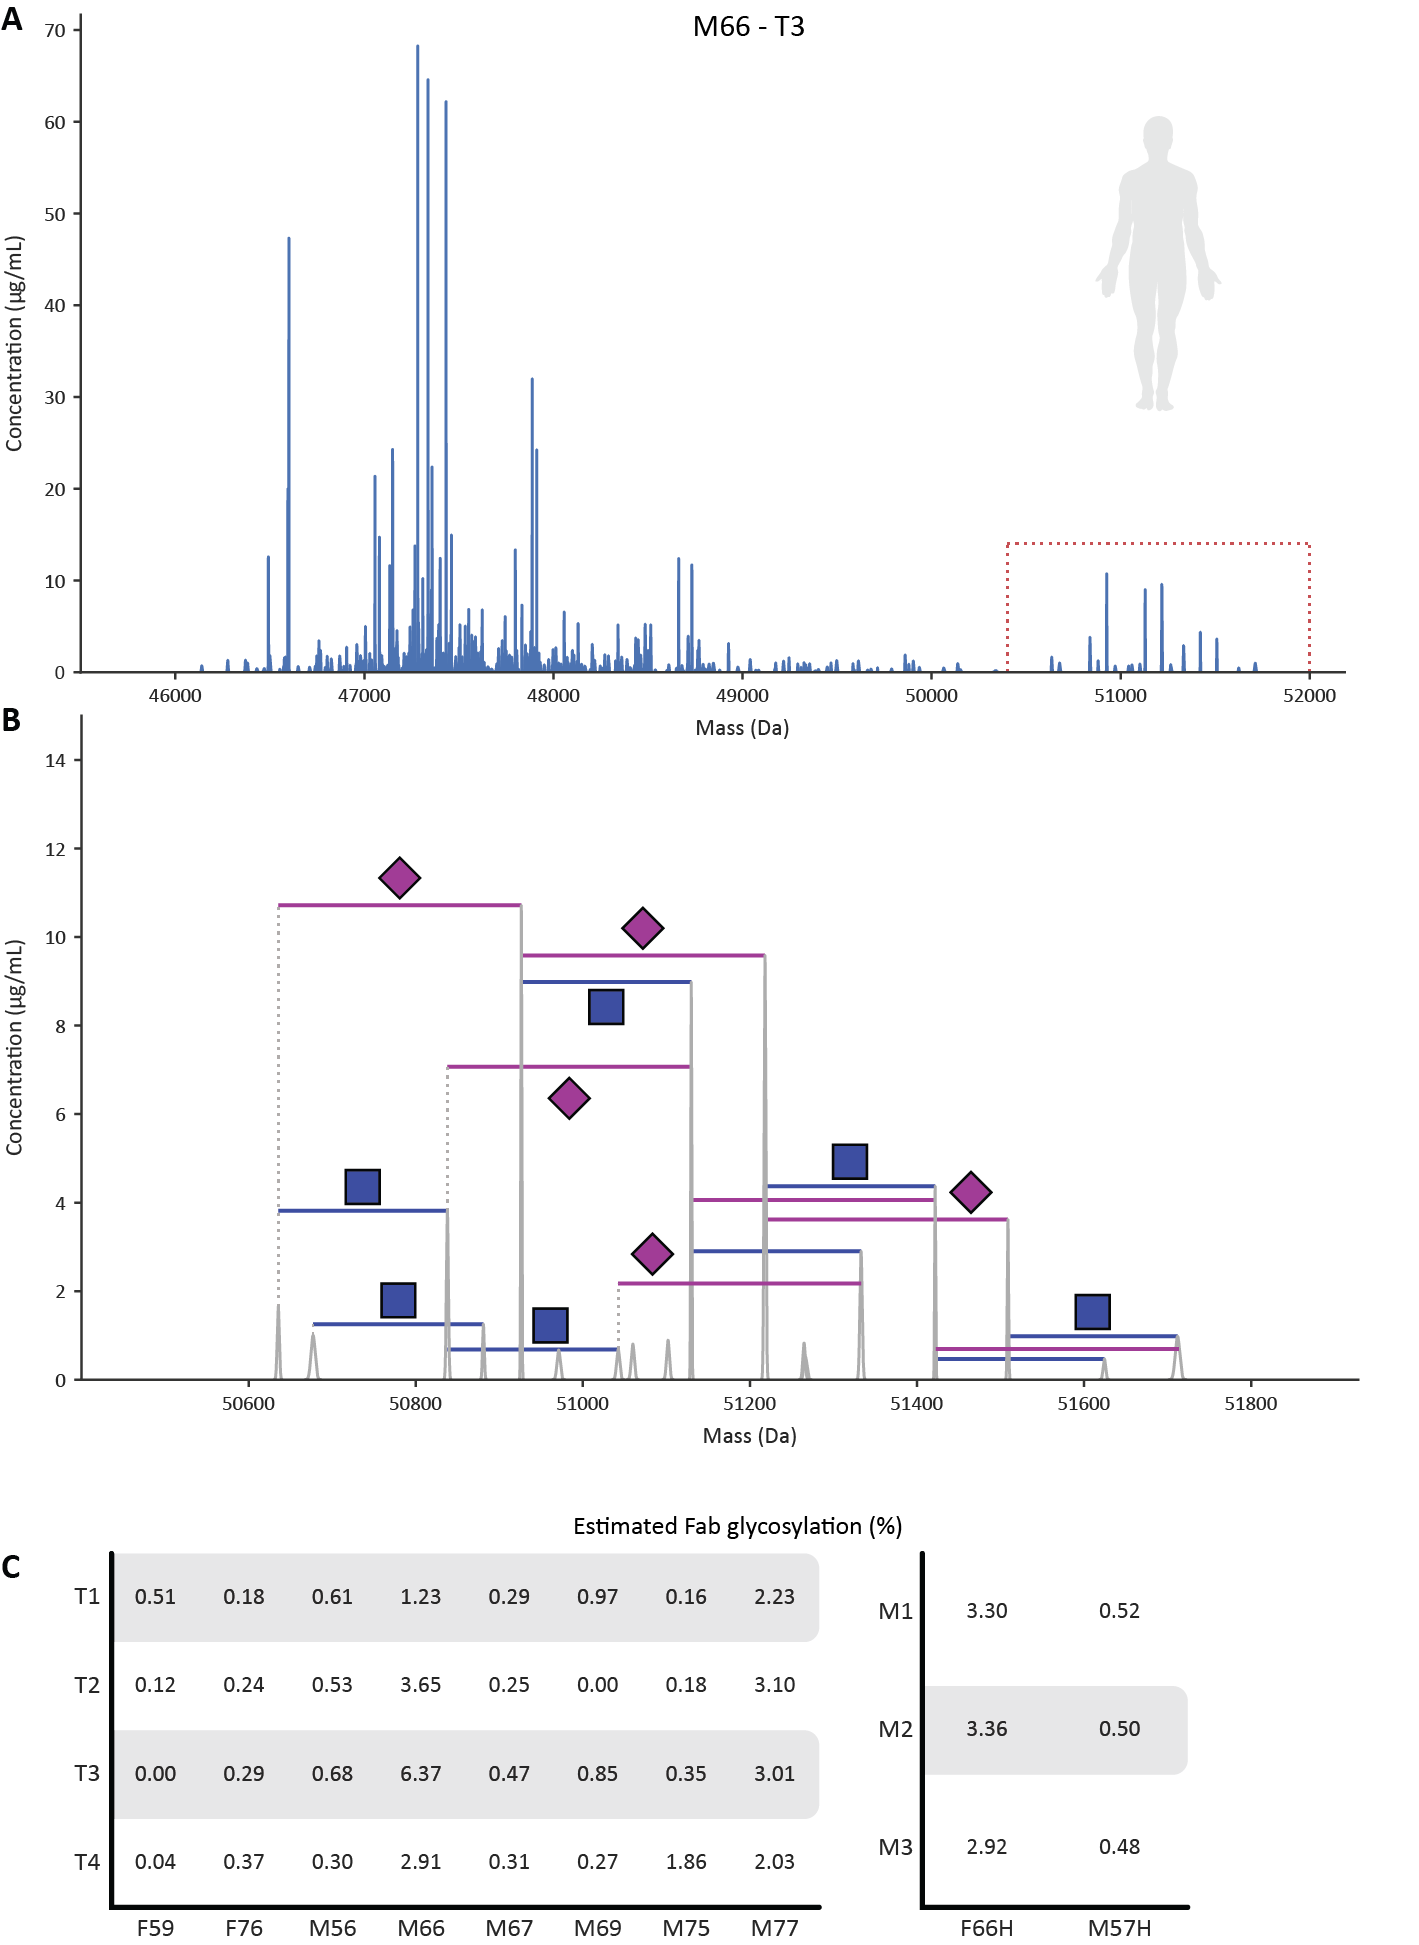
\includegraphics[]{Chapter.3/Figures/fs2.png}
    \captionsetup{singlelinecheck = false, format= hang}
    \caption{
      Figure legend on next page.
    }
    \label{fig:figs3.2}
  \end{figure*}
  \addtocounter{figure}{-1}
  \begin{figure*}[pt!]
    \caption{
      \textbf{Extent of Fab glycosylation in the plasma repertoire} ~~a) Fab mass profile of donor M66, taken from the plasma sample at time point 3. The mass range between 50,400 Da and 52,000 Da is boxed in red and shown magnified in panel ~~b) . ~~b) Zoomed-in mass profile with annotation of glycan-related masses. Monosaccharides mass differences between peaks are annotated as follows: blue square = GlcNAc (203 Da), magenta diamond = sialic acid (291 Da). For annotation of the glycosylation a mass tolerance of 1 Da and a retention time tolerance of 0.6 min was used. ~~c) Estimated percentages of plasma Fab molecules being glycosylated in all samples measured. For this, Fab clones with a mass >49,500 Da were assumed to carry one or more Fab glycans. This value was chosen because the in silico Fab distribution generated from the IMGT database (shown in \textbf{\autoref{fig:figs3.1}d}) extends up to 49,500 Da, the majority of Fabs has a mass between 47,000 and 48,000, and the average literature described Fab glycan has a mass of approximately 2,300 Da. The validity of this assumption is illustrated for M66 – T3 in panels ~~a) with the glycosylated Fabs being in mass quite separated from the other clones. The percentage of plasma Fab molecules being glycosylated was calculated by taking the sum of Fab concentrations above 49,500 Da and dividing these by the total detected concentration in each sample. On the left in ~~c) are shown the \% Fab glycosylation in the plasmas of the septic patients, on the right the \% observed in two healthy donors. In general, we observe that the \% Fab glycosylation is < 1\%, although in some donors it is substantially higher, i.e. M66, M77 and F66H.
    }
    \vspace{24cm}
  \end{figure*}
  \begin{figure*}[!hbt]
    \center
    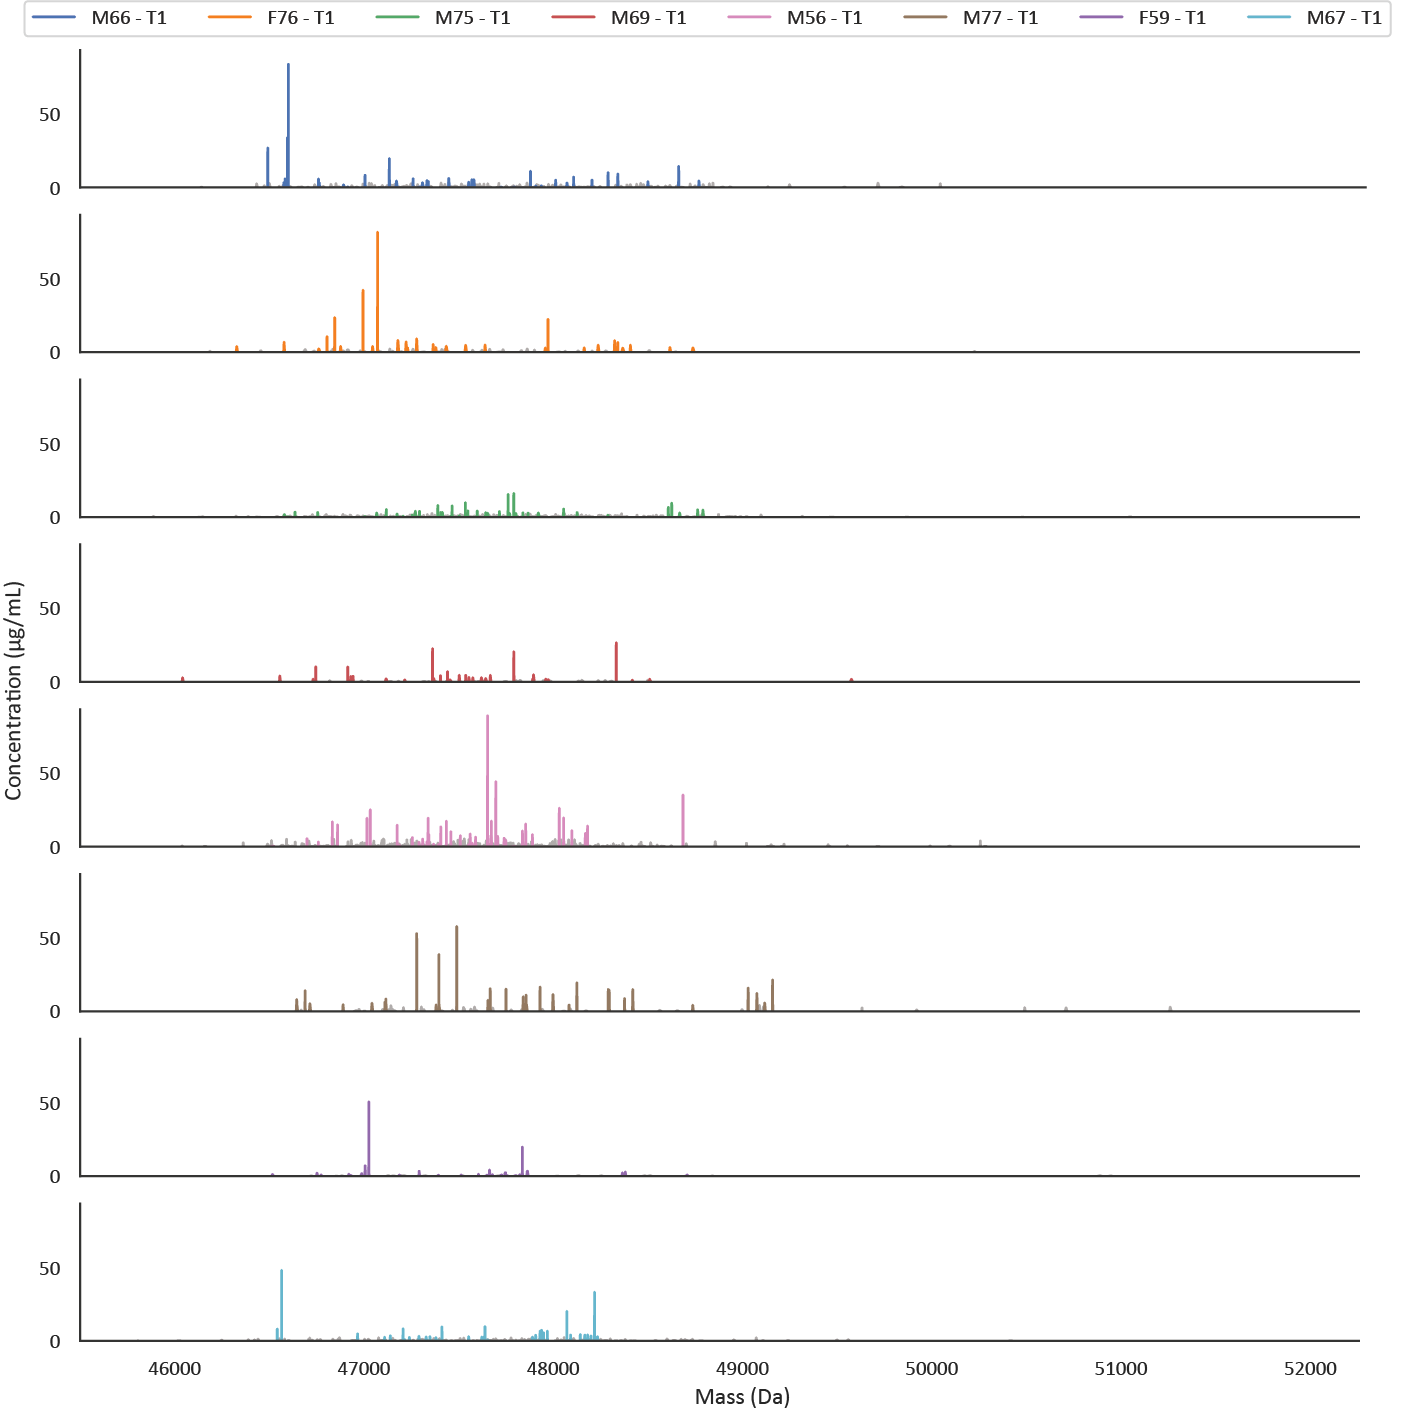
\includegraphics[]{Chapter.3/Figures/fs3.png}
    \caption{
      \textbf{Fab mass profiles are simple and uniquely individual.} The by LC-MS obtained Fab mass profiles are shown for plasma taken from each patient at time point 1 (post-operative). The Fab mass profiles are plotted along the full mass range. In each profile the top 30 most intense clones are colored, with a separate color for each donor. The remaining clones are shown in grey. The concentrations were determined from the LC-MS intensities, normalized against two spiked in recombinant mAbs.
    }
    \label{fig:figs3.3}
  \end{figure*}

  \vspace{1cm}

  \begin{figure*}[!p]
    \center
    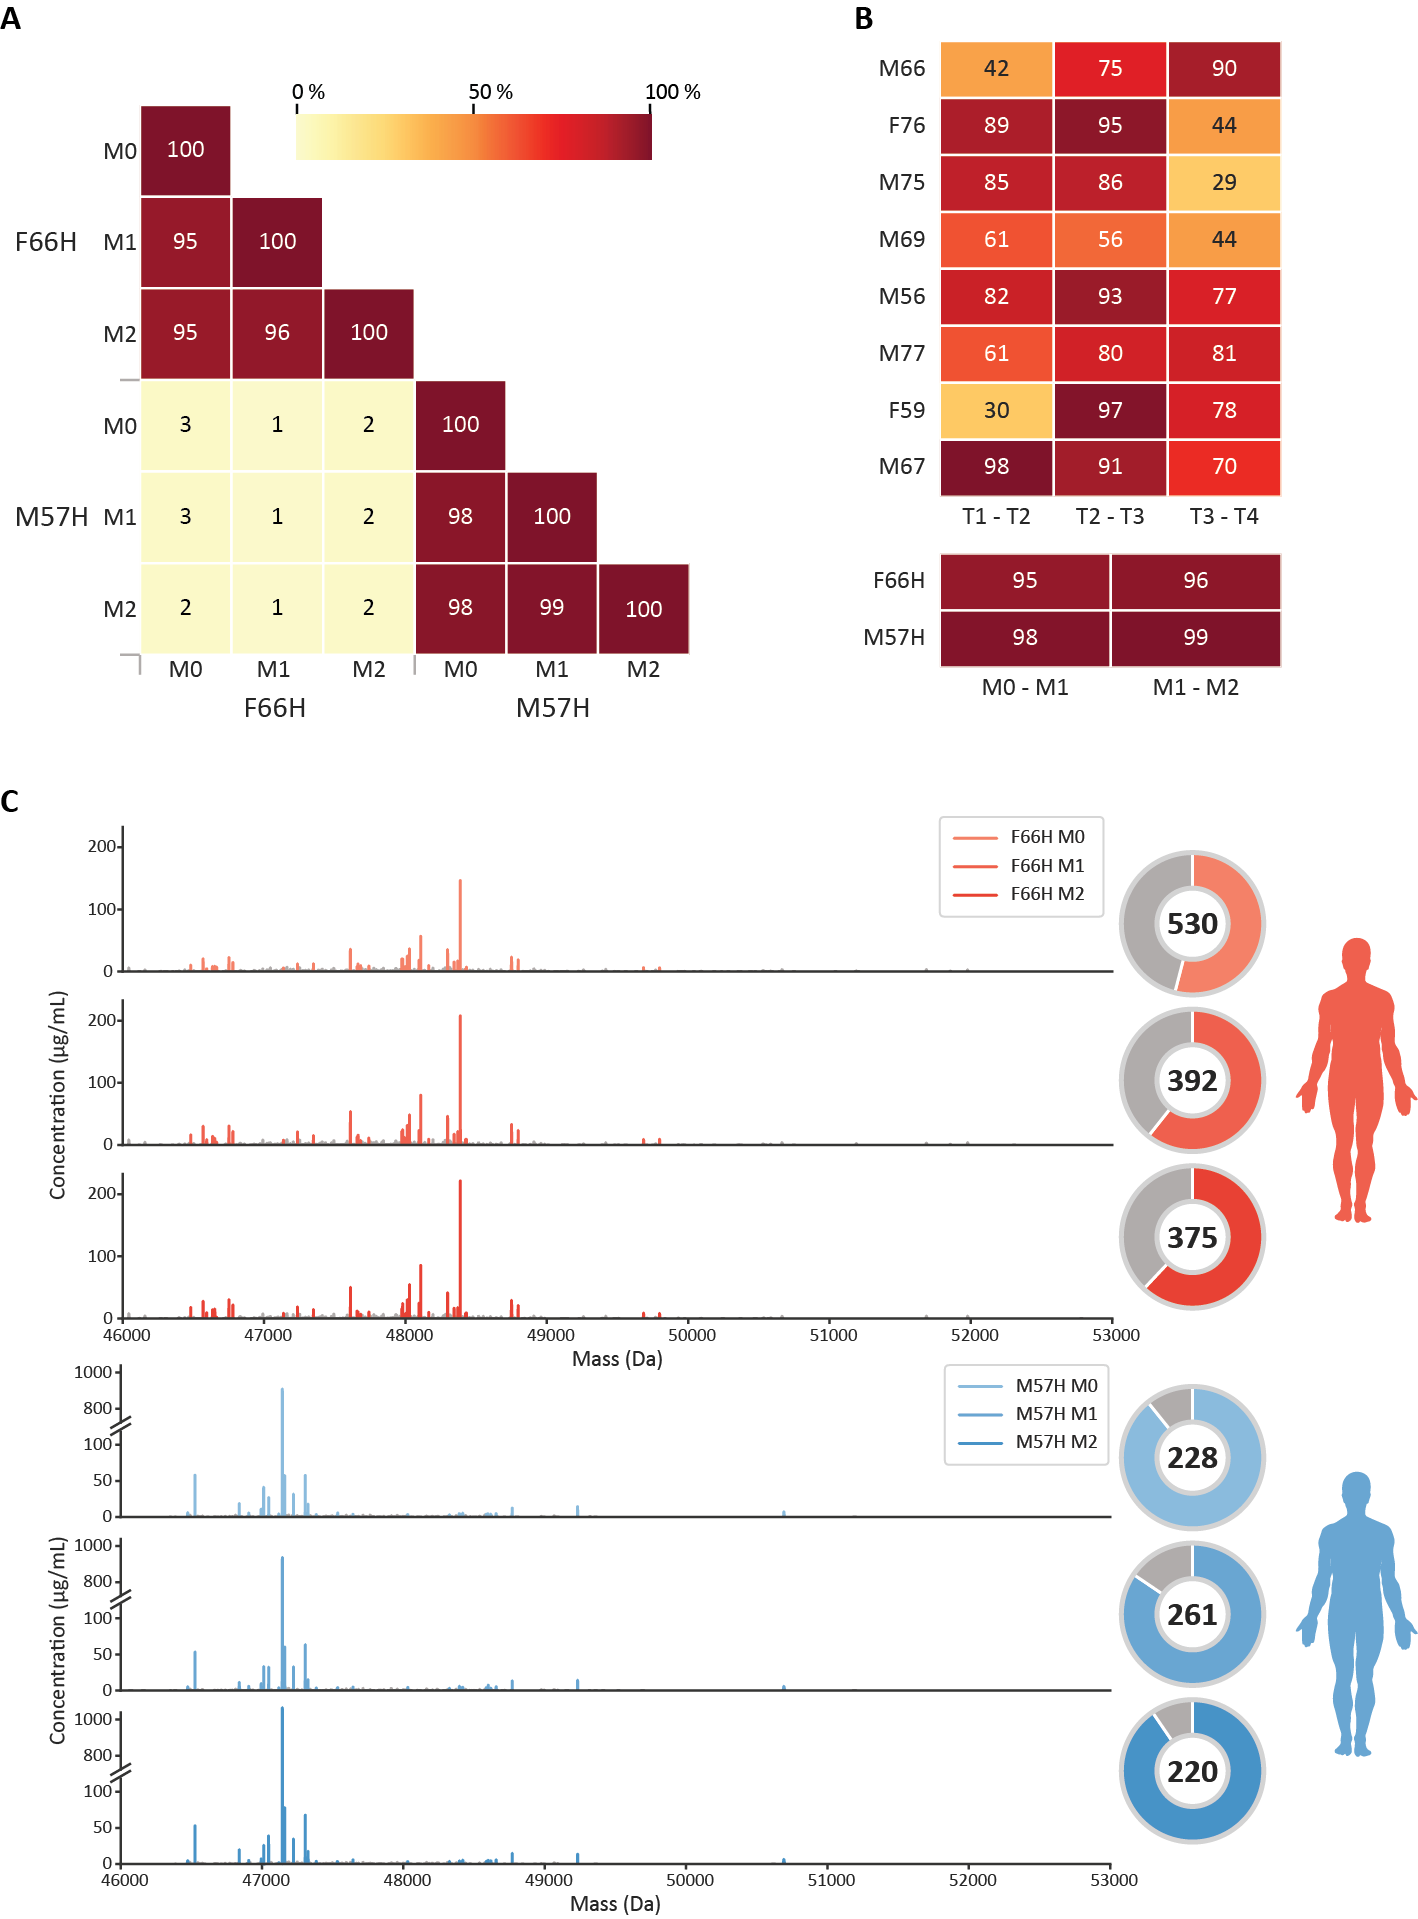
\includegraphics[]{Chapter.3/Figures/fs4.png}
    \captionsetup{singlelinecheck = false, format= hang}
    \caption{
      Figure legend on next page.
    }
    \label{fig:figs3.4}
  \end{figure*}
  \addtocounter{figure}{-1}
  \begin{figure*}[pht!]
    \caption{
      \textbf{Longitudinal plasma Fab profiles obtained for two healthy donors.} ~~a) Heatmap of healthy donors F66H and M57H constructed using the same method as used in \textbf{\autoref{fig:fig3.2}a}. Time points are marked M0, 1, and 2, representing month 0, month 1 and month 2, to clearly distinguish these from the sepsis donor time points. Inside each cell of the heatmap a percentage value shows the degree of overlap between samples, which is also represented by the color bar. ~~b) Heatmap showing the Fab overlap in consecutive time points of all healthy and sepsis affected donors, showing only the degree of overlap for consecutive time points within each donor. The colors match those of the color bar from panel A. ~~c) Mass profiles of healthy donors with donut charts. For each mass profile the top 30 most intense clones are colored, and the remaining clones are colored grey. In the donut charts the colored slice displays the distribution of the top 30 most intense clones compared to the other clones. The value inside the donut shows the total number of detected clones.
    }
  \end{figure*}

  \vspace{1cm}
  \begin{figure*}[!hbt]
    \center
    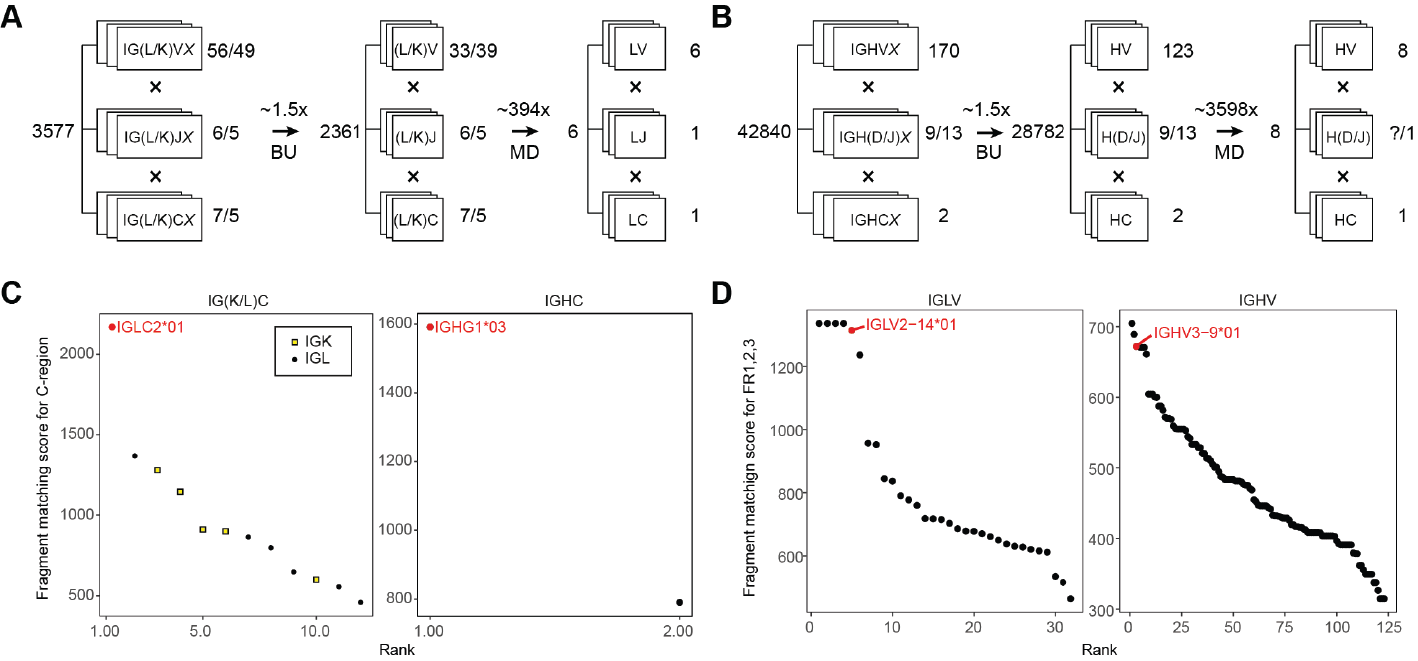
\includegraphics[]{Chapter.3/Figures/fs5.png}
    \caption{
      \textbf{Template matching of the obtained sequencing data for the Fab clone \textsuperscript{24.4} 1 \textsubscript{47359.4} versus the IMGT database.} The filtering of IMGT database and scoring of the germline IGXV and IGXC-alleles was performed by using iteratively bottom-up (BU) and middle-down (MD) proteomics data. ~~a) Filtering of germline IGL and IGK alleles with BU and MD mass spectrometry (MS) reduces the number of possible germline light chain sequences from 3,577 to 6 candidate sequences ($\sim$600-fold reduction). ~~b) Filtering of germline IGH alleles with BU MS and MD MS reduces the number of possible germline heavy chain sequences from 42,840 to 8 candidate sequences ($\sim$5,000-fold reduction). ~~c) Fragment matching scores for the germline C-gene alleles of the light (left) and heavy (right) chain of the Fab clone \textsuperscript{24.4} 1 \textsubscript{47359.4} using the middle-down MS data. ~~d) Fragment matching scores for the Framework Regions 1, 2, and 3 of the germline V-gene alleles of light (left) and heavy (right) chains of IgG1 determined by using the middle-down MS data.
    }
    \label{fig:figs3.5}
  \end{figure*}

  \vspace{1cm}

  \begin{figure*}[!ht]
    \center
    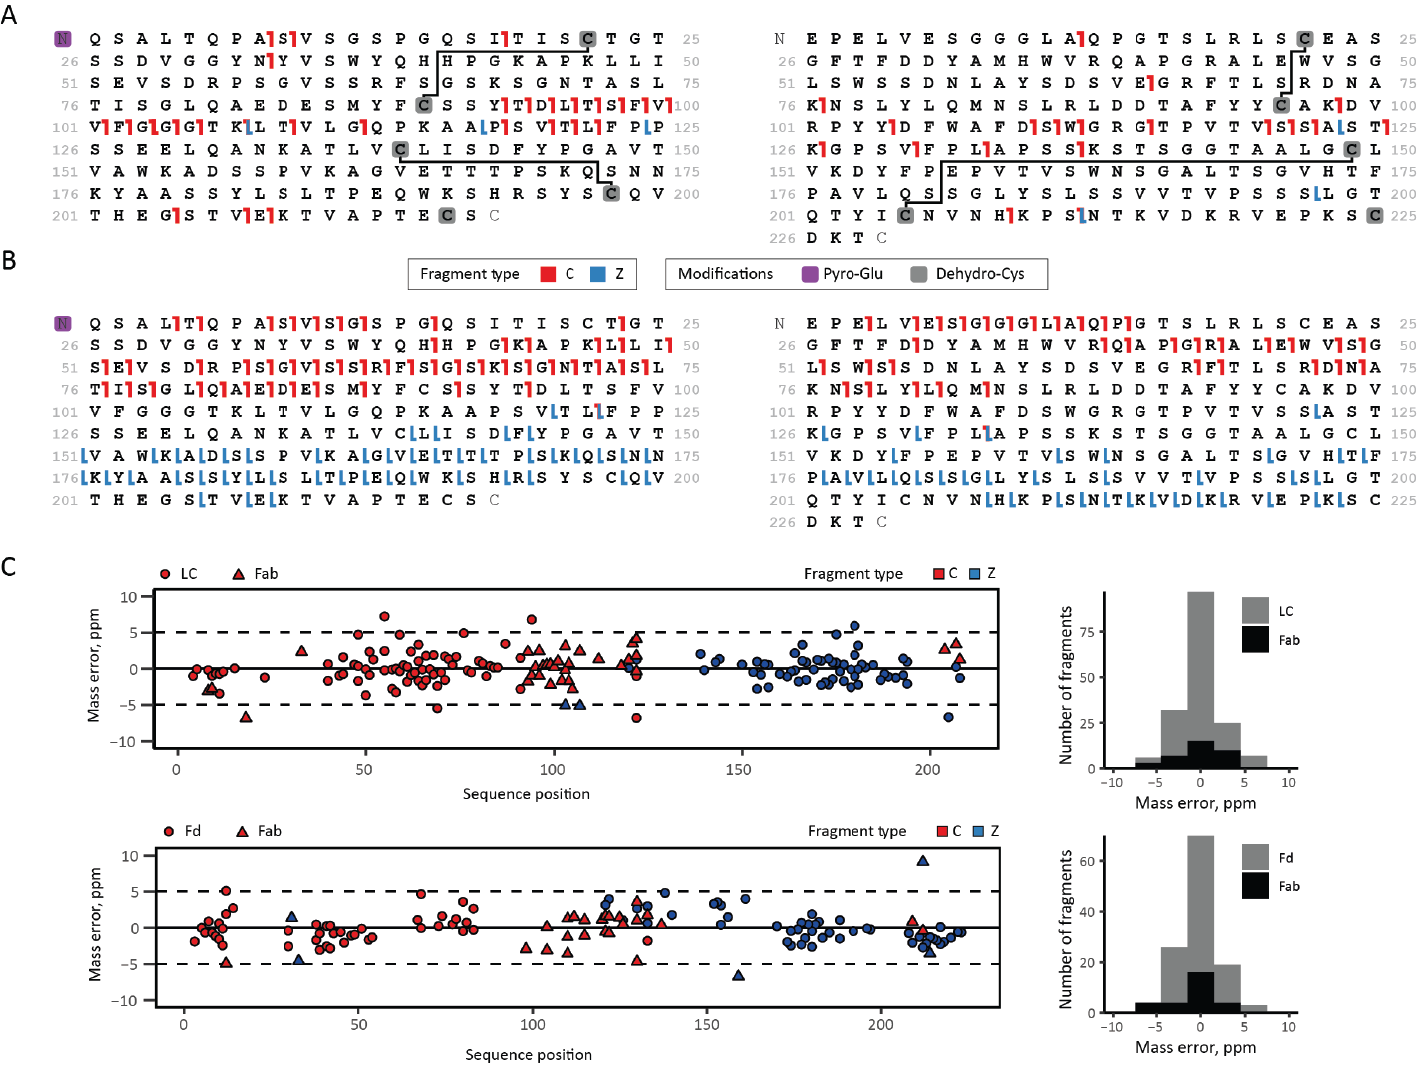
\includegraphics[]{Chapter.3/Figures/fs6.png}
    \caption{
      \textbf{Middle-down ETD analysis and sequence annotation of the light chain and the N-terminal portion of the
        heavy chain from clone \textsuperscript{24.4} 1 \textsubscript{47359.4} from donor F59.} ~~a) Fragmentation maps of the light chain (left) and Fd (right) when subjected to ETD within the intact Fab molecule. ~~b) Fragmentation maps of the light chain (left) and Fd (right) when subjected to ETD after reduction and denaturation of the precursor Fab. ~~c) Mass errors and their distribution of the light chain fragments observed in ETD of Fab and the light chain alone, and mass errors and distribution thereof for Fd fragments detected in ETD of Fab and Fd alone.
    }
    \label{fig:figs3.6}
  \end{figure*}

  \vspace{1cm}

  \begin{figure*}[!ht]
    \center
    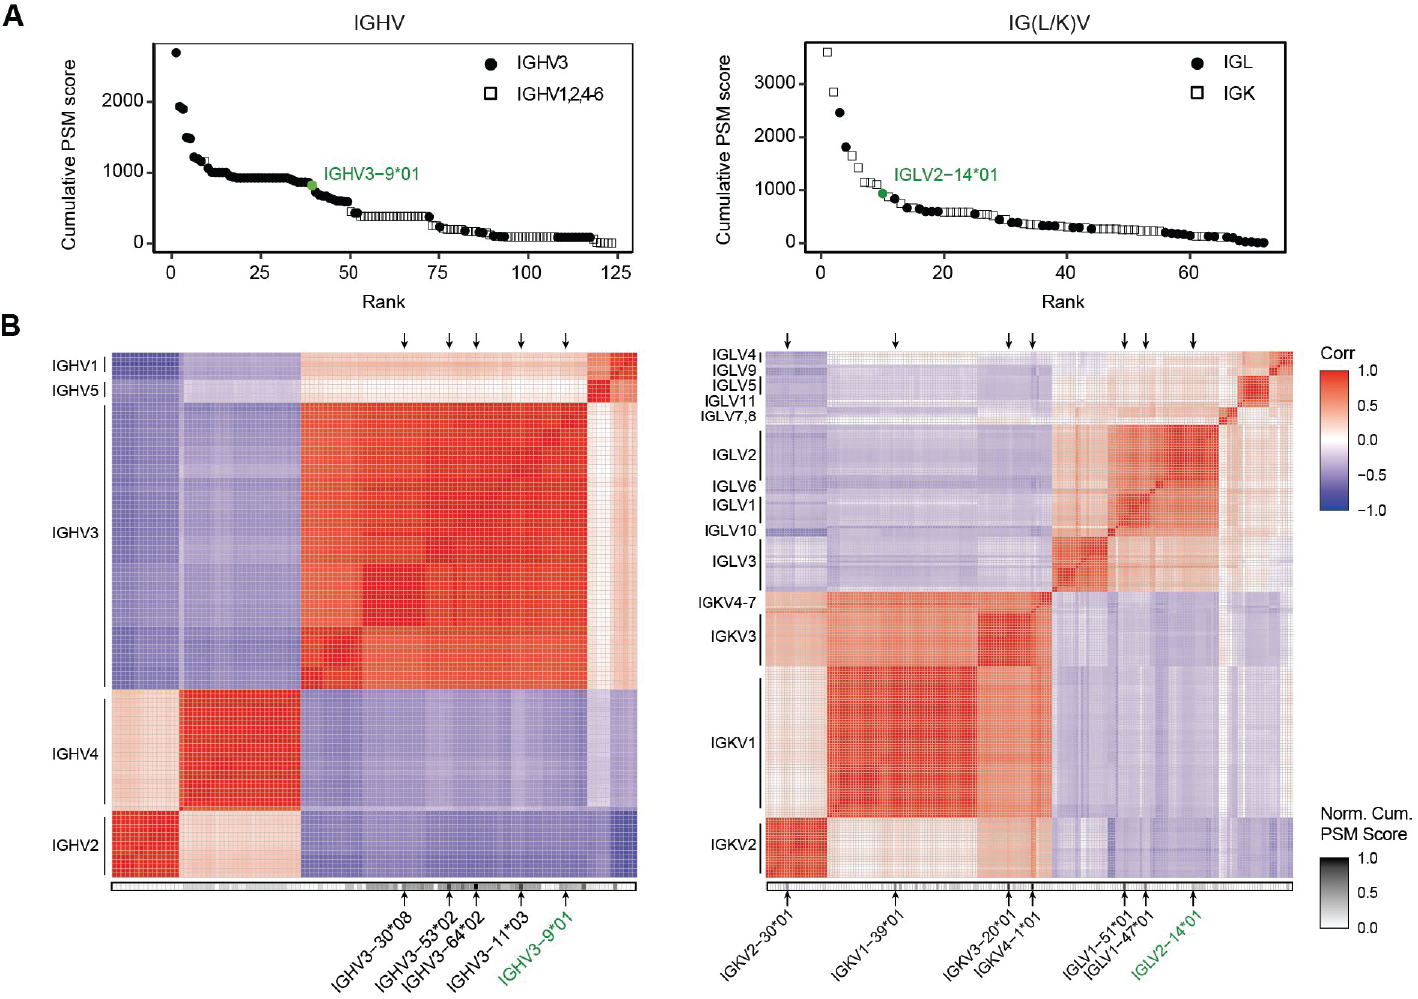
\includegraphics[]{Chapter.3/Figures/fs7.png}
    \caption{
      \textbf{Large homologous families of Ig V-gene alleles (e.g. IGHV3) are observed among the top-scoring identifications as extracted from the bottom-up proteomics data.} ~~a) Cumulative PSM scores determined for the germline V-gene alleles of the Fab heavy (left) and light chains (right). On the left, alleles from the largest IGHV3 family are displayed as filled circles; alleles of other IGHV families are shown as empty squares. On the right, alleles from larger and more homologous IGKV families are shown as empty squares, while filled circles display alleles of IGLV families. Germline V-gene sequences were downloaded from IMGT. ~~b) Correlation matrix displaying sequence similarity among all germline V-gene sequences of the Fab heavy (left) and light (right) chain. Normalized cumulative PSM scores are shown below the correlation maps. Some of the top-scoring V-gene sequences are indicated with black arrows. The V-genes ultimately determined for clone \textsuperscript{24.4} 1 \textsubscript{47359.4} by the integrative \emph{de novo} bottom-up and middle-down sequencing are highlighted in green.
    }
    \label{fig:figs3.7}
  \end{figure*}

  \vspace{1cm}

  \begin{figure*}[!ht]
    \center
    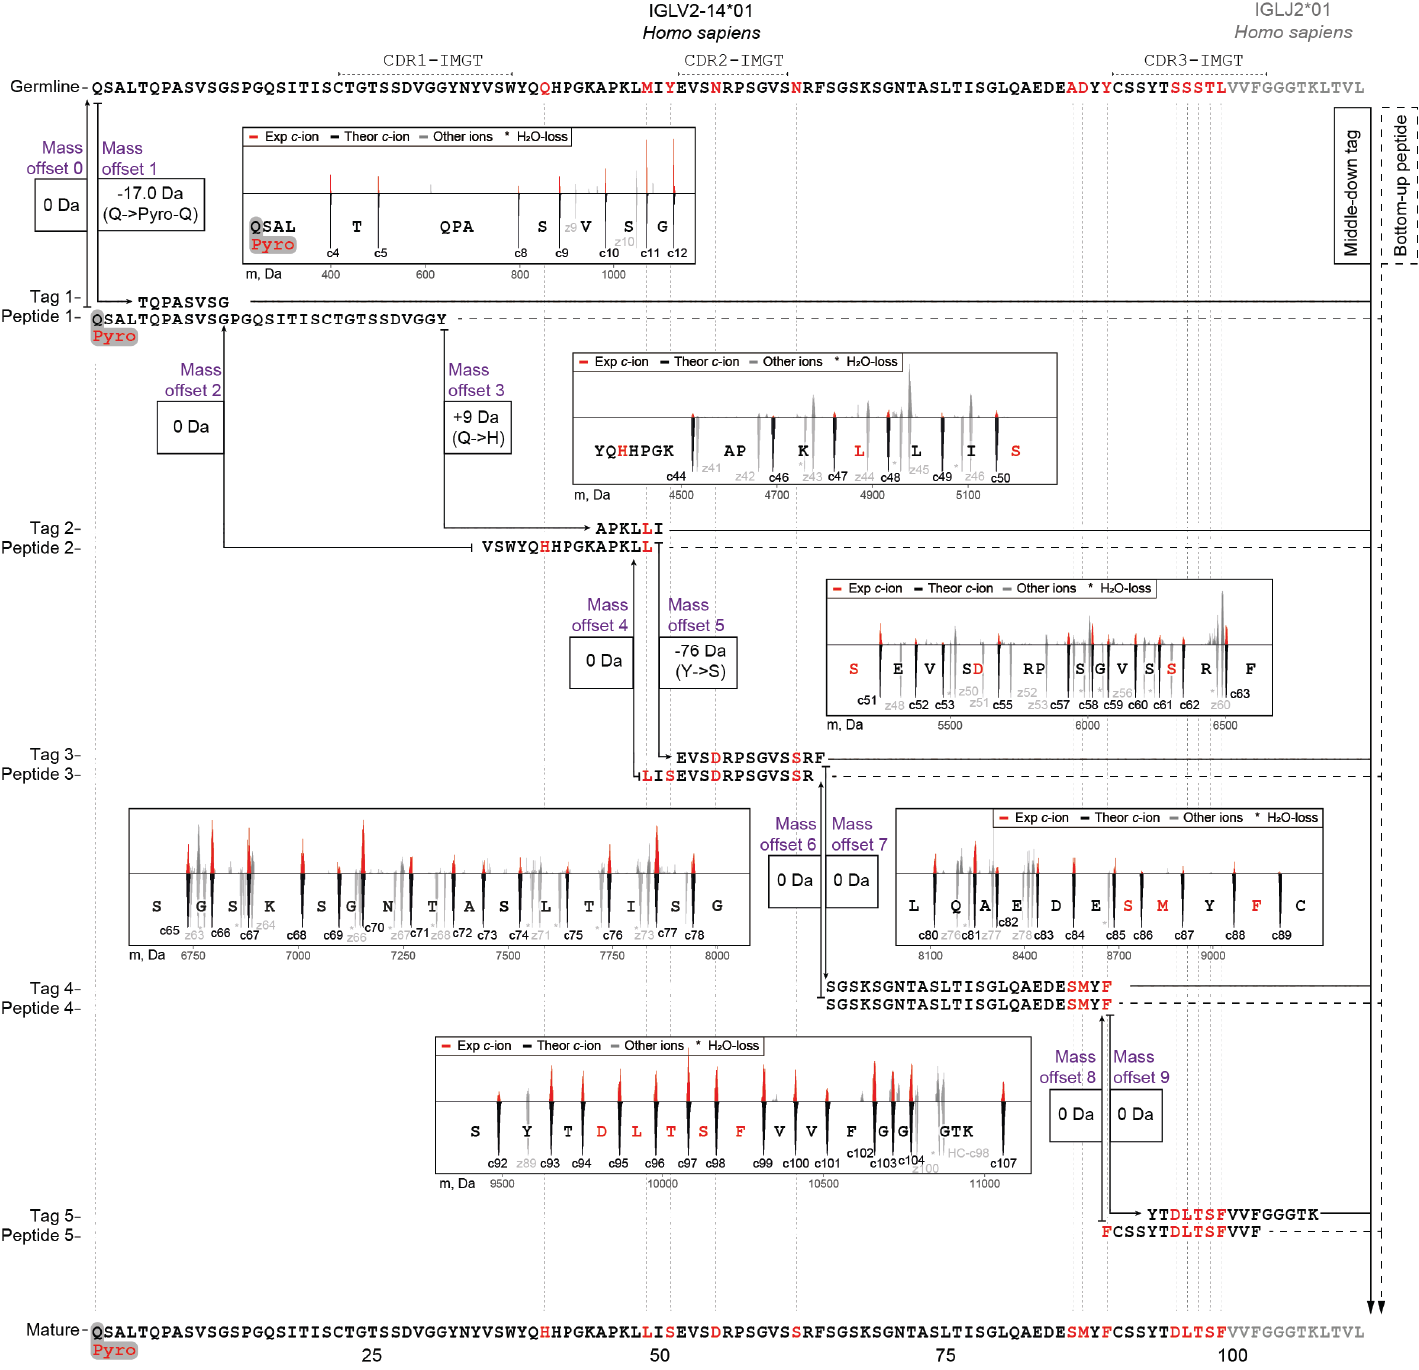
\includegraphics[]{Chapter.3/Figures/fs8.png}
    \caption{
      \textbf{Refining of the sequence of clone \textsuperscript{24.4} 1 \textsubscript{47359.4} light chain germline IGLV2-14$\star$01-IGLJ2$\star$01, based on the iterative integration of middle-down and bottom-up proteomics data.} ~~a) First, the sequence tags detected in the middle-down MS data were used as arrays of consecutive fragment peaks, which directly hinted at the presence of 11 mutations (M49L, Y51S, Y51S, N55D, N62S, A85S, D86M, Y88F, S95D, S96L, S97T, T98S, and L99F). Next, these tags were aligned to the \emph{de novo} sequenced peptide sequences obtained by bottom-up MS, revealing 2 additional mutations. The highest scoring aligned peptides were used to extend the initial sequence tags, and then these steps were iteratively repeated. At each step of tag extension, the mass offsets were calculated by comparing a mass gap between two consecutive tags to the mass of amino acid residues in the corresponding gap in the germline sequence. Iteratively, middle-down tags were extended with aligning peptides until all (if possible) mass offsets become equal to 0 Da. Eventually, 13 mutations and one modified residue (Pyro-Q) were determined for the \textsuperscript{24.4} 1 \textsubscript{47359.4} light chain sequence. De-charged isotopic distributions of the fragments involved in each sequence tag are displayed as red peaks in the corresponding insets with the theoretical isotopic distributions for these fragments displayed underneath each fragment. Fragmentation spectra of the peptides used in this refining process for the CDRs are shown in \textbf{\autoref{fig:fig3.5}}. See also \textbf{\autoref{tab:tabdummy3.5}}. for an overview of the evidence supporting each detected amino acid mutation.
    }
    \label{fig:figs3.8}
  \end{figure*}

  \vspace{1cm}

  \begin{figure*}[!ht]
    \center
    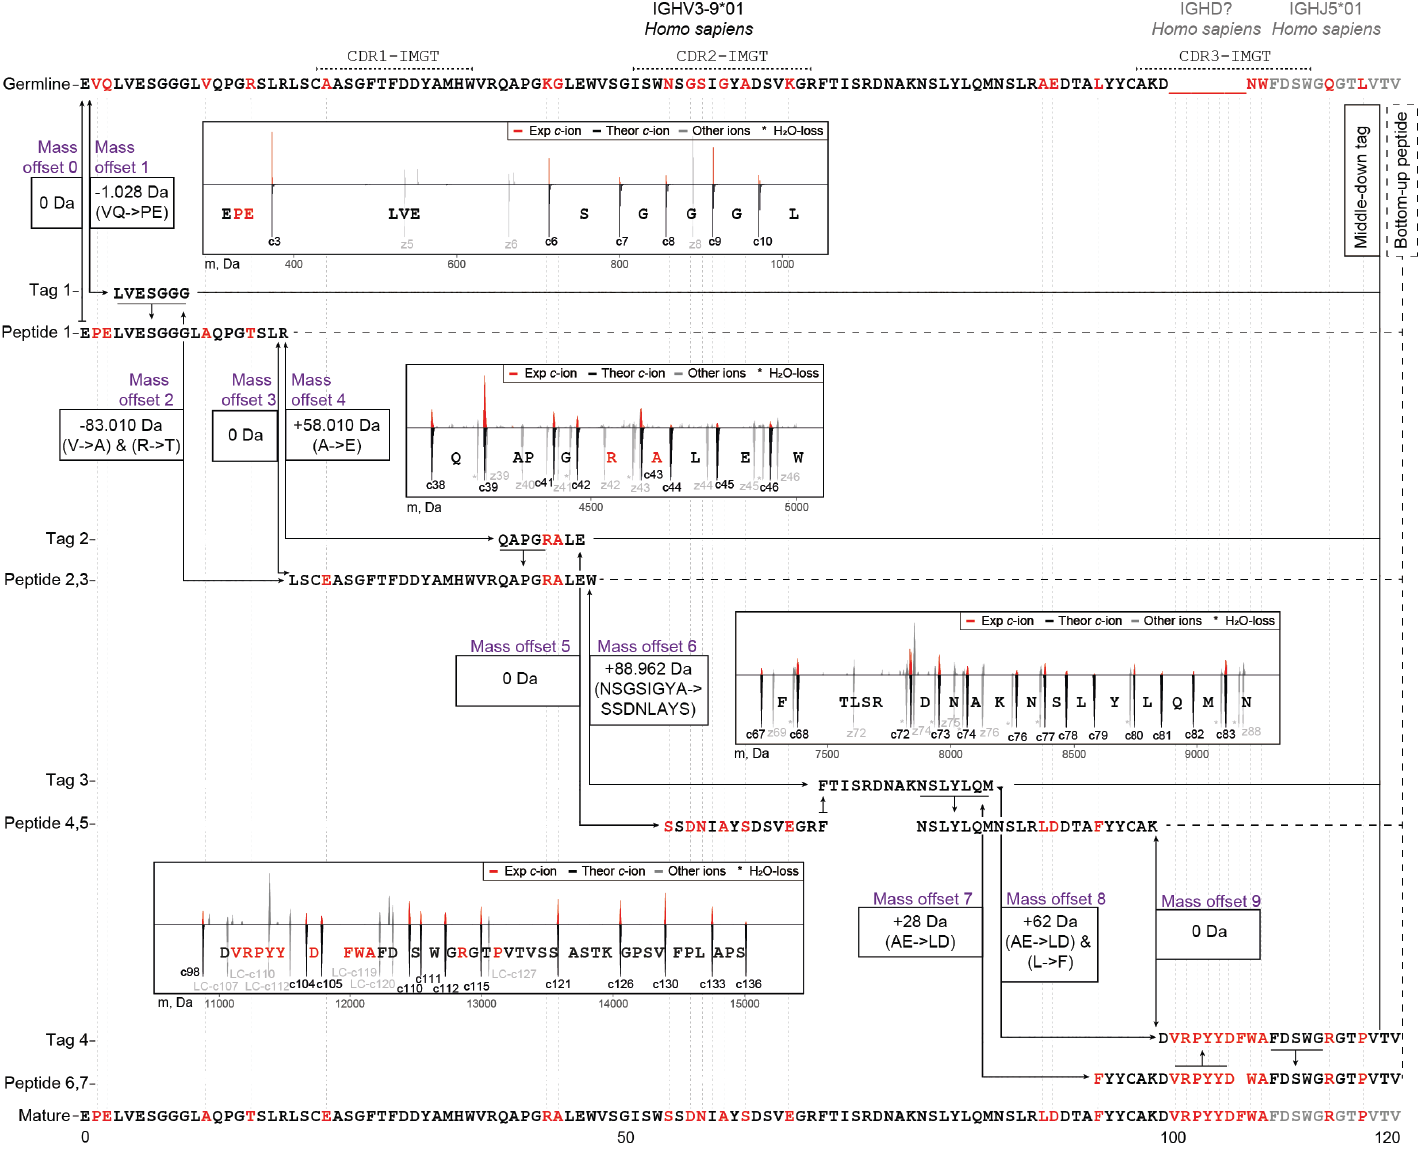
\includegraphics[]{Chapter.3/Figures/fs9.png}
    \caption{
      \textbf{Refining of the sequence of clone \textsuperscript{24.4} 1 \textsubscript{47359.4} heavy chain germline IGHV3-9$\star$01-IGHJ5$\star$01, based on the iterative integration of middle-down and bottom-up proteomics data.} ~~a) First, sequence tags were detected in the middle down MS data as arrays of consecutive fragment peaks similar to refining of the light chain. Next, these tags were aligned to the \emph{de novo} sequenced peptides from bottom-up MS. The highest-scoring aligned peptides were used to extend the initial tags, and then this step was repeated. At each step of tag extension, the mass offsets were calculated by comparing a mass gap between two consecutive tags to the mass of amino acid residues in the corresponding gap in the germline sequence. Iteratively, tags were extended with aligning peptides until all (if possible) mass offsets become equal to 0 Da. Eventually, more than 20 mutations were determined for the N-terminal portion of the heavy chain for clone \textsuperscript{24.4} 1 \textsubscript{47359.4}. De-charged isotopic distributions of the fragments involved in each sequence tag are displayed as red peaks in the corresponding insets with the theoretical isotopic distributions for these fragments displayed underneath each fragment. Fragmentation spectra of the peptides used in this refining process for the CDRs are shown in \textbf{\autoref{fig:fig3.5}}.
    }
    \label{fig:figs3.9}
  \end{figure*}

  \vspace{1cm}

  \begin{figure*}[!ht]
    \center
    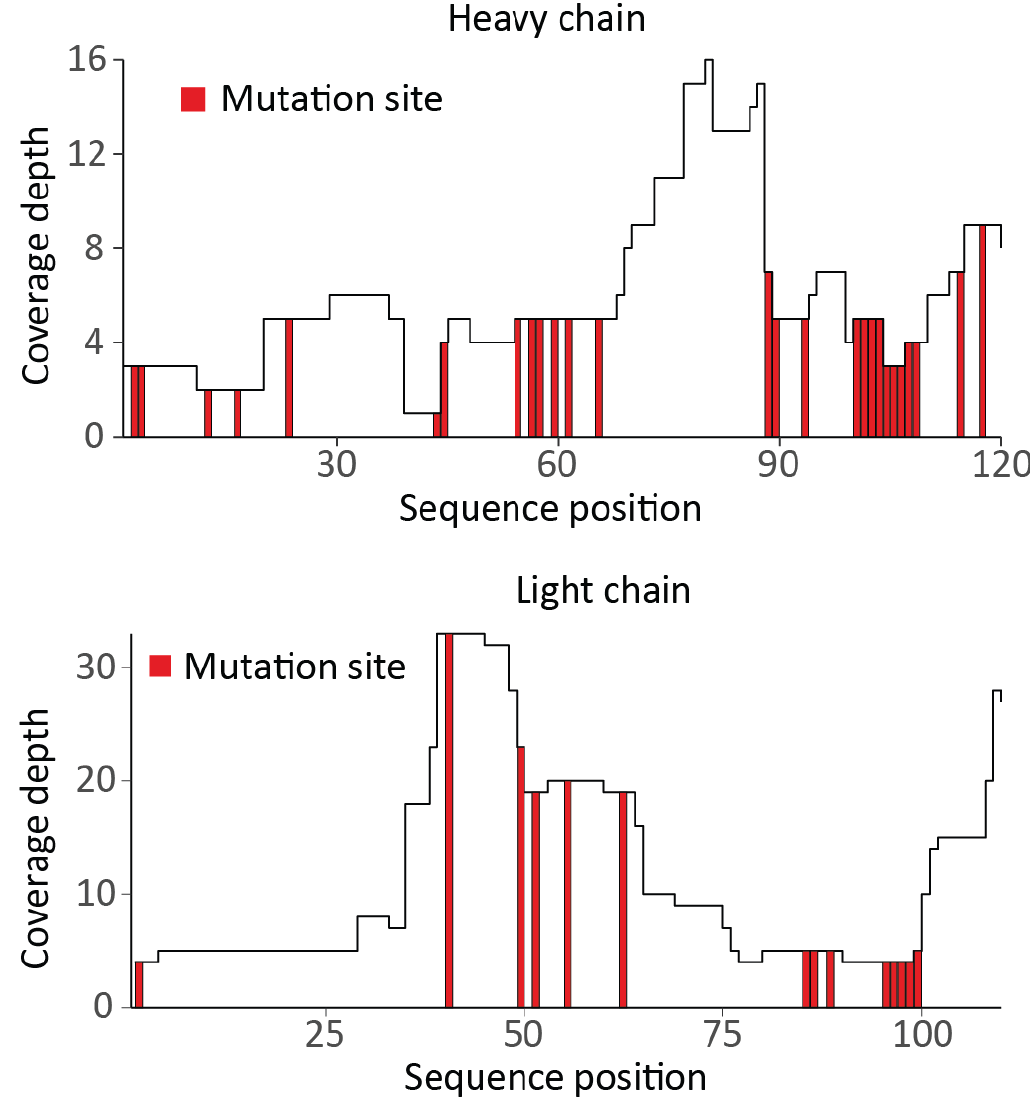
\includegraphics[]{Chapter.3/Figures/fs10.png}
    \caption{
      \textbf{Coverage depths for \emph{de novo} sequenced light and heavy chains of the clone \textsuperscript{24.4} 1 \textsubscript{47359.4} from donor F59.} ~~a) Values at each position represent the number of unique peptides identified in the bottom-up LC-MS/MS data. The determined mutation sites are depicted in red. Only the first 110 and 120 amino acids are shown for the light and heavy chain, respectively.
    }
    \label{fig:figs3.10}
  \end{figure*}

\end{subappendices}

\clearpage
\section*{References}
\bibliographystyle{Stylesettings/pnas}
\patchcmd{\thebibliography}
{\clubpenalty 4000\widowpenalty 4000}
{\clubpenalties 1 10000 \widowpenalties 1 10000}
{}{}
\bibliography{chapmerge}
\stopthumb



\picturechapter{A case series exploring the human milk polyclonal IgA1 response to repeated SARS-CoV-2 vaccinations by LC–MS based fab profiling}{Chaptercovers/ch4.pdf} \label{ch-4}
\vspace*{0.25cm}

{\footnotesize Sebastiaan C. de Graaf, Albert Bondt, Danique M.H. van Rijswijck, Hannah G. Juncker, Sien J. Mulleners, Mirjam J.A. Damen, Max Hoek, Britt J. van Keulen, Johannes B. van Goudoever, Albert J.R. Heck, Kelly A. Dingess}
%%
\begin{center}
  \vspace{3cm}
  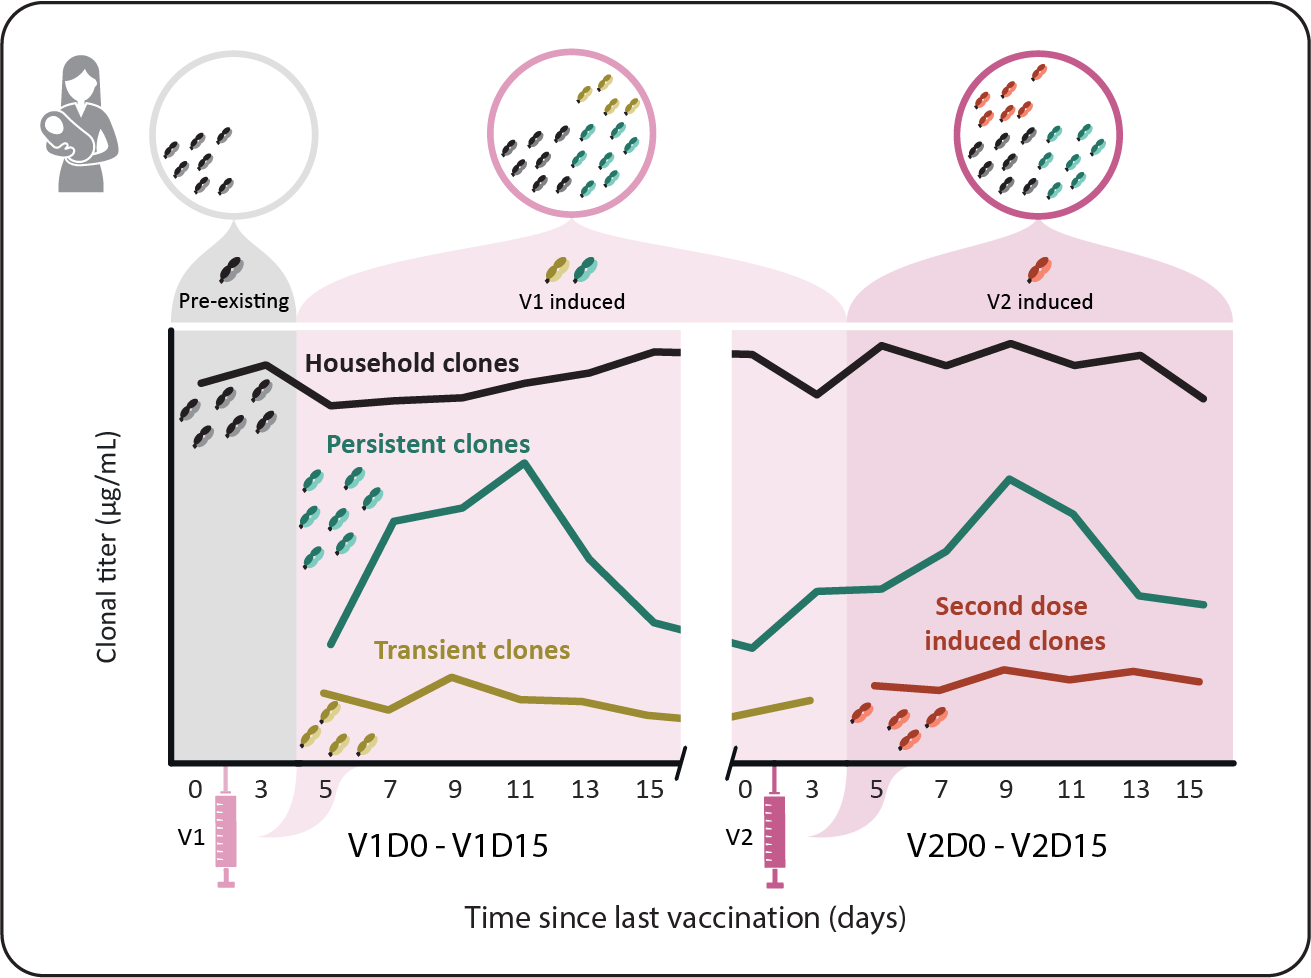
\includegraphics[]{Chapter.4/Figures/Ch4.png}
  \vspace{0.25cm}
\end{center}

\begin{flushleft}
  \vspace*{\fill}
  \rule{\textwidth}{1pt}\\[0cm]
  \textbf{This chapter is based on work in the following publication:}\\
  \footnotesize
  \textbf{\emph{Frontiers in Nutrition}} (2024), 10:1305086, doi:10.1016/j.mcpro.2023.100690\\
\end{flushleft}

\begin{abstract102}
  Upon vaccination against severe acute respiratory syndrome coronavirus 2 (SARS-CoV-2) humans will start to produce antibodies targeting virus specific antigens that will end up in circulation. In lactating women such antibodies will also end up in breastmilk, primarily in the form of secretory immunoglobulin A1 (SIgA1), the most abundant immunoglobulin (Ig) in human milk. Here we set out to investigate the SIgA1 clonal repertoire response to repeated SARS-CoV-2 vaccination, using a LC-MS fragment antigen-binding (Fab) clonal profiling approach. We analyzed the breastmilk of six donors from a larger cohort of 109 lactating mothers who received one of three commonly used SARS-CoV-2 vaccines. We quantitatively monitored the SIgA1 Fab clonal profile over 16 timepoints, from just prior to the first vaccination until 15 days after the second vaccination. In all donors, we detected a population of 89-191 vaccine induced clones. These populations were unique to each donor and heterogeneous with respect to individual clonal concentrations, total clonal titer, and population size. The vaccine induced clones were dominated by persistent clones (68\%) which came up after the first vaccination and were retained or reoccurred after the second vaccination. However, we also observe transient SIgA1 clones (16\%) which dissipated before the second vaccination, and vaccine induced clones which uniquely emerged only after the second vaccination (16\%). These distinct populations were observed in all analyzed donors, regardless of the administered vaccine. Our findings suggest that while individual donors have highly unique human milk SIgA1 clonal profiles and a highly personalized SIgA1 response to SARS-CoV-2 vaccination, there are also commonalities in vaccine induced responses.
\end{abstract102}
\thumbforchapter

\section{Introduction}
\lettrine[lraise=0.1, nindent=0em, slope=-.5em]{I}{mmunoglobulins} (Ig), or antibodies, are a key part of the adaptive immune response capable of specifically recognizing and binding to antigens derived from bacteria or viruses initiating and aiding in their neutralization. Every individual has a unique antibody repertoire generated by a magnitude of distinct antibody-producing B cells, with estimates ranging from 10\textsuperscript{13} to 10\textsuperscript{18} \cite{briney2019commonality, schroeder2006similarity}. Throughout our lives these repertoires are built up by encountering a huge variety of pathogens and other foreign stimuli, which we are exposed to daily or at specific moments in time, such as vaccines. However, at a given moment in time there are likely only hundreds to thousands of different detectable antibodies in human serum and milk, and typically the top 50 most abundant Ig clones account for up to 90\% of the complete Ig repertoire \cite{bondt2021human, bondt2021direct, dingess2023identification}.
In our first moments of life, we begin to build this repertoire and are provided passive immunity through breastfeeding, receiving in most cases our mother’s own unique antibodies. After natural infection with severe acute respiratory syndrome coronavirus 2 (SARS-CoV-2), SARS-CoV-2 specific antibodies with neutralizing capacity are present in human milk and are thought to provide immunity to infants \cite{dong2020antibodies, fox2020robust, pace2021characterization, keulen2021human, bode2022characterization, lebrão2020early, juncker2021human}. The advantages of breastfeeding and the absence of vertical transmission of SARS-CoV-2 via human milk \cite{dong2020antibodies, pace2021characterization, kumar2022sars-cov-, krogstad2021no, chambers2020evaluation} have led to the advice of the WHO to encourage mothers to continue breastfeeding their infant during the COVID-19 pandemic \cite{organization2020breastfeeding}. Recently, several SARS-CoV-2 vaccines have been widely administered to people around the world. While the accumulated evidence has shown that these vaccines are safe and effective also for pregnant and lactating women \cite{juncker2021comparison, zilver2023vaccination, fu2022systematic, jamieson2022update, shimabukuro2021preliminary, falsaperla2021covid-}, this more vulnerable group was excluded from initial SARS-CoV-2 vaccine trials. Therefore, information regarding vaccine driven antibody development in lactating women is still rather limited. This information is beneficial for breastfeeding women to make a well-informed decision regarding vaccination to confer protection to not only themselves, but also their immune naïve infant \cite{simon2015evolution}. The most abundant Ig in human milk is IgA at a concentration of 1.0-2.6 g/L being 10 to 100 times greater than IgG and IgM respectively \cite{czosnykowska-łukacka2020changes, lönnerdal2017longitudinal}. IgA comes in two subclasses IgA1 and IgA2, with IgA1 typically being the more abundant subclass in human milk. We recently developed methods to study IgA1 clonal repertoires in human serum and milk. After affinity-purification, all IgA (IgA1 and IgA2) molecules from human serum or milk \cite{bondt2021direct, dingess2023identification} become bound to the affinity resins, whereafter we use specific enzymes to cleave IgA1 molecules selectively, yielding the fragment antigen binding (Fab) domains that harbor the complementarity determining regions. These Fabs are then subjected to intact mass analysis by LC-MS clonal profiling. This yields a clonal profile that typically contains several hundred unique clones, each identified by a specific LC-MS signature based on mass and retention time. We can quantify the human milk concentrations of each Fab clone by spiking in recombinant IgA1 mAb standards \cite{bondt2021direct}, enabling us to monitor the abundance of individual clones over time. Monitoring the human milk IgA1 clonal repertoire of healthy individuals, we observed that they are relatively simple, being dominated by just a few hundred to thousand different clones at a given time. These repertoires are unique and highly personalized as we do not observe the same clones in more than one donor. Furthermore, we found the human milk IgA1 repertoires of healthy donors to be very stable over time \cite{bondt2021direct}, whereas the clonal repertoires of individuals that experience serious illness, can undergo distinct and sudden changes \cite{bondt2021human, rijswijck2022discriminating}.
Mothers that were previously infected with SARS-CoV-2 have significantly higher concentrations of spike specific IgA in their breastmilk than negative controls \cite{keulen2021human}, and using LC-MS we were able to detect spike specific secretory IgA1 (SIgA1) Fab fragments in these donors. Interestingly, concentrations of spike specific IgA in human milk had little correlation with neutralization capability, and spike specific SIgA1 Fabs were of a relatively low concentration when compared to total SIgA1 in human milk. Other studies have also shown weak correlations between antibody titers and the frequency of recirculating memory B cells relative to a respective antigen \cite{wolf2022antibody}. These findings suggest that high concentrations of antibodies may not be good predictors for effective viral recognition and binding. Detailed knowledge about the emergence and evolution of antibodies in response to vaccination could render better insights into the immunity they provide and thereby yield better predictors for its longevity and effectivity.
Here, we aim to expand the knowledge about the antibody response of lactating women following SARS-CoV-2 vaccination by investigating the SIgA1 profiles of six individuals that received repeated mRNA-based or vector-based SARS-CoV-2 vaccines. Donors and their samples for this observational longitudinal case series were selected from a previously described cohort \cite{juncker2022comparing}. Using LC-MS Fab clonal profiling, we monitored the abundance of individual SIgA1 clones and studied the antibody response at a clonal level of detail. Novel in this study is that we use computational methods to detect SIgA1 Fab clonal populations emerging after vaccination by eliminating all clones that were present before a response to vaccination could be expected. The human milk SIgA1 clonal repertoires of six individual donors receiving one of three SARS-CoV-2 vaccines were longitudinally (at 16 timepoints), quantitatively monitored. All six donors had unique SIgA1 clonal repertoires in which longitudinal changes were observed, with novel clonal populations emerging after both the initial and second vaccination. Our data reveals that antibody responses to vaccination are highly personalized traits and argues for monitoring antibody responses beyond the total Ig titer level, using a more detailed, personalized, and longitudinal approach.
\begin{figure*}[!pt]
  \center
  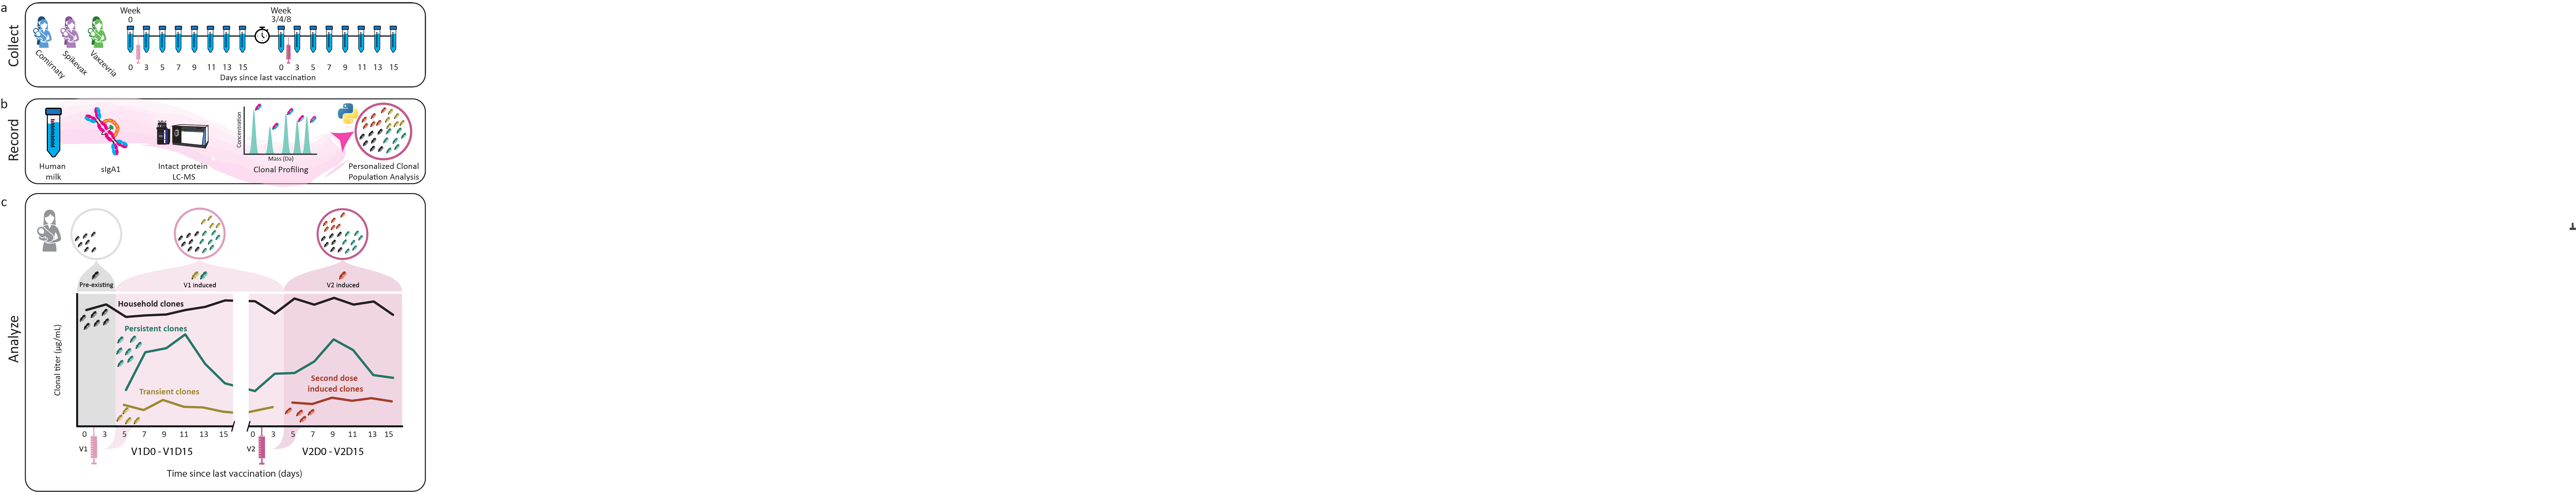
\includegraphics[]{Chapter.4/Figures/f1.png}
  \captionsetup{singlelinecheck = false, format= hang}
  \caption{
    Figure legend on next page.
  }

  \label{fig:fig4.1}
  \vspace{24cm}

\end{figure*}

\addtocounter{figure}{-1}

\begin{figure*}[!ht]
  \caption{\textbf{Study Workflow.} ~~a) Human milk samples were obtained from six donors across 16 timepoints, from just prior to the first vaccination until 15 days after the second vaccination. Individual donors received one of three vaccines, BNT162b2/Comirnaty (blue), mRNA-1273/Spikevax (purple) or AZD1222/Vaxzevria (green). The sample collections are indicated by the tubes and each vaccination with a syringe. The clock indicates the gap in time between vaccinations. ~~b) SIgA1 was affinity-purified from human milk. Subsequently, proteolytically formed SIgA1 Fab fragments were separated and analyzed by LC-MS to obtain a list of clones (i.e., Fab molecules with a unique mass/retention time pair). The concentration of each clone was retrieved at the sampled timepoints using two recombinant IgA internal standards. Clones were then assigned to populations based on their window of detection relative to vaccination, and these populations were analyzed for each donor individually. ~~c) Illustrative examples of abundance profiles of clonal populations over time. The y-axis shows the clonal titer (i.e., the summed concentrations of the clones) for each population over time. Timepoints are referred to as for example V1D3, where D3 indicates the number of days since the last vaccination and V1 indicates the last vaccination. Clones were assigned to one of four populations based on their detection window relative to vaccination. The black line represents \emph{household} clones, SIgA1 clones that were detected in one of the first two timepoints, before a response to vaccination could be expected based on analysis of the parent cohort. All other clonal population were absent from these time points and are considered vaccine induced clones. The remaining three populations designated are \emph{persistent} (teal), \emph{transient} (mustard) and \emph{second dose induced} (maroon) clones. The transient population consists of clones that are only detected in the window V1D5 - V2D3. The persistent clones are clones that arise in the window V1D5 - V2D3 and are also detected after V2D3. Clones in the second dose induced population are clones that were not observed until after V2D3.}
\end{figure*}


\section{Results}

\subsection{Vaccination results in a heterogeneous polyclonal response}
In this observational longitudinal case series, we recorded the human milk SIgA1 clonal profiles of six individual donors receiving either Comirnaty, Spikevax or Vaxzevria vaccines (\textbf{\autoref{fig:fig4.1}}). We detected a total of 2553 clones across all donors, ranging between 229 and 505 unique clones per donor (\textbf{\autoref{fig:fig4.2}a}), excluding clones that were only found at a single timepoint from all subsequent analysis to limit false discoveries. In line with our previous studies, there was virtually no overlap in the clonal repertoire between donors (only a single clone had an overlapping mass and retention time between donors). In contrast, overlap within each individual donor over the longitudinal sampling was exceptionally high (over 95\% of clones were detected at more than one timepoint).\\
\begin{figure*}[!htp]
  \center
  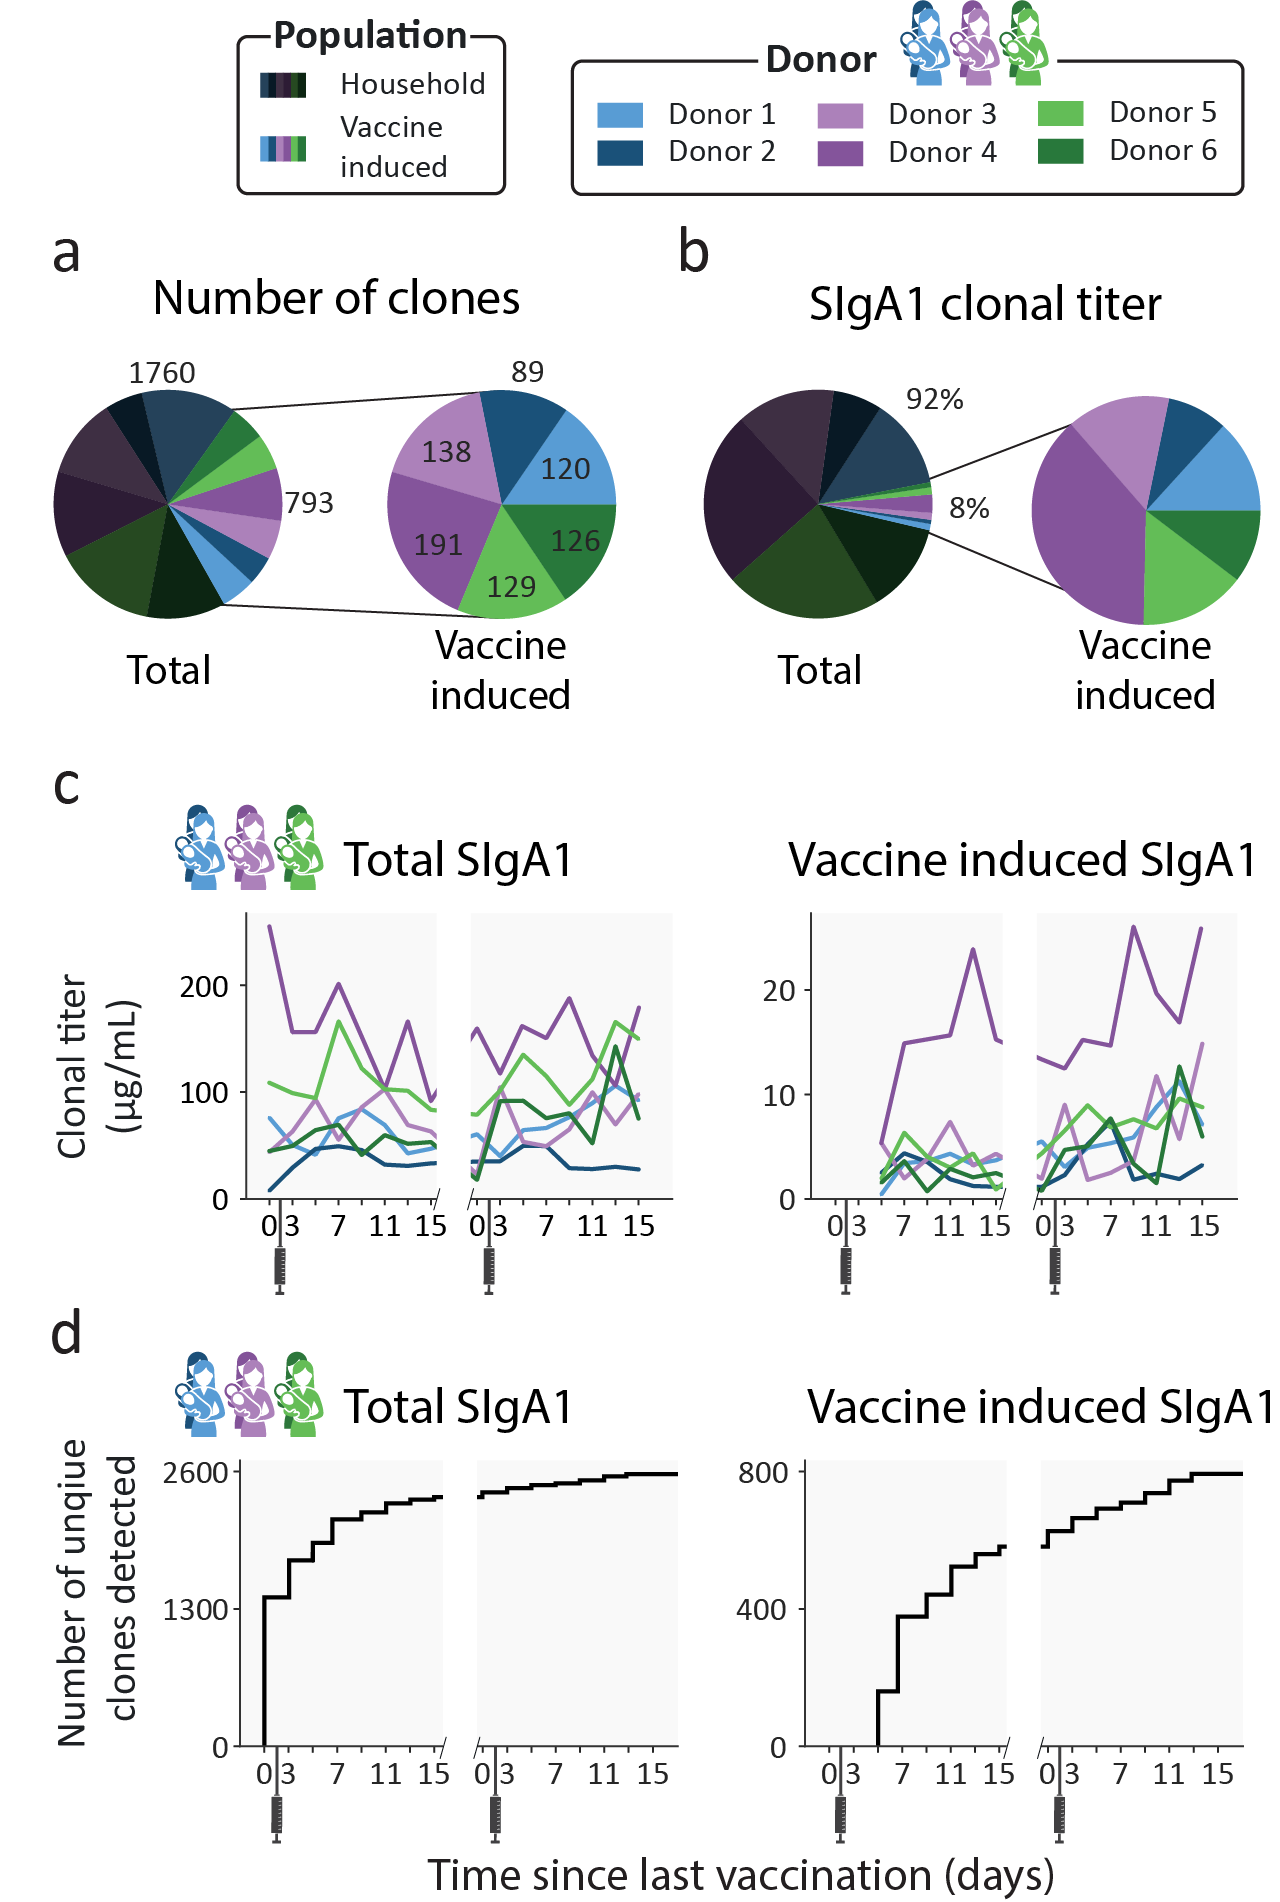
\includegraphics[]{Chapter.4/Figures/f2.png}
  \caption{\textbf{Emergence of novel clones after vaccination.} ~~a) Pie charts showing the number of unique clones designated as household (dark) and vaccine induced (light), colored per donor. Vaccine induced clones made up 31\% of all detected clones (793 out of 2553 clones). ~~b) Pie charts showing the percent total abundance the household clones (dark) and vaccine induced clones (light), colored per donor. ~~c) Longitudinal changes in total SIgA1 clonal titer (left) and vaccine induced SIgA1 clonal titers (right) for each donor. Vaccine induced SIgA1 clonal titers rise in response to the repeated vaccinations and make up an average of 7\% of the total SIgA1 clonal titer. ~~d) Total number of unique clones detected over time (left) and number of unique vaccine induced clones (right). Novel clones emerge shortly after vaccination and by day 7 nearly half of all vaccine induced clones (377 out of 793) have been detected.
  }
  \label{fig:fig4.2}
\end{figure*}

For all donors, the SIgA1 clonal repertoire was dominated by abundant clones that were already detected in the first (V1D0) or second (V1D3) milk sample, before a clonal response is expected as it is prior to or too close to vaccination, as also confirmed based on ELISA data \cite{juncker2022comparing} (\textbf{\autoref{fig:figs4.1}}). These clones, which we term \emph{household} clones (\textbf{\autoref{fig:fig4.1}c, \autoref{fig:figs4.2}}), accounted for 92\% of the total SIgA1 \emph{clonal titer} (the summed abundance of all clones) of all samples combined (\textbf{\autoref{fig:fig4.2}b}) and 83-99\% of the total SIgA1 clonal titer in any single sample. In each donor, we detected between 89 and 191 clones that emerged more than 3 days after the first vaccination (V1D5 and later) (\textbf{\autoref{fig:fig4.2}a}). These clones, which we termed \emph{vaccine induced clones} (\textbf{\autoref{fig:fig4.1}c,} \textbf{\autoref{fig:figs4.2}}), made up 31\% of the total detected clones (793 out of 2553 clones, \textbf{\autoref{fig:fig4.2}a}). These vaccine induced clones were comparatively low in abundance and made up a relatively small portion of the total SIgA1 clonal titer per sample (\textbf{\autoref{fig:fig4.2}c}). Most of the vaccine induced clones emerged shortly after the first vaccination was administered: 47\% of the vaccine induced clones (377 clones), were first observed between V1D5 and V1D7 (\textbf{\autoref{fig:fig4.2}d}). This agreed with the ELISA findings for these same samples, where anti-spike SIgA titers started rising around day 5, and further sharp increases were observed 9 days after vaccination (\textbf{\autoref{fig:figs4.1}}).

\subsection{Novel clonal populations emerge after the second vaccination in all donors}
As the vaccines the donors received consist of two doses, we defined four clonal populations based on the window of detection relative to both vaccinations (\textbf{\autoref{fig:fig4.1}c,} \textbf{\autoref{tab:tabs4.1}}). The first population we termed above as \emph{household} clones. These are SIgA1 clones that were detected before a clonal response was expected, at V1D0 or V1D3. The previously described \emph{vaccine induced} clones were categorized into three distinct populations: \emph{transient, persistent}, and \emph{second dose induced} clones. The transient and persistent populations are both made up of clones that were detected before timepoint V2D3 but were absent at the first two timepoints (V1D0 and V1D3). The transient clones were \emph{only} detected in the time window from V1D5 to V2D3. Persistent clones arose in this same time window but were \emph{also} detected after V2D3. Clones in the second dose induced population are clones that were first observed after V2D3.
These four populations were observed in all donors. Persistent clones were the largest population: 21\% of all detected clones were persistent clones (539 clones, \textbf{\autoref{fig:fig4.3}a}), and persistent clones made up between 50 and 80\% of donor specific vaccine induced clones (\textbf{\autoref{fig:fig4.3}b}). The transient and second dose induced populations were much smaller and more diverse. The transient and second dose induced populations each make up 5\% of all clones (126 and 128 clones respectively, \textbf{\autoref{fig:fig4.3}a}), and 5-20\% and 5-27\% of donor specific vaccine induced clones (\textbf{\autoref{fig:fig4.3}b}) respectively. When looking at the fractional clonal titer (i.e., the proportion a population contributed to the total SIgA1 clonal titer at a single timepoint) over time, the behavior of these populations was remarkably similar between donors (\textbf{\autoref{fig:fig4.3}c}). The persistent clones dominated here too, as they made up the bulk of the vaccine induced clonal titer at nearly all timepoints and on average of 5.9\% of the total SIgA1 clonal titer. Transient and second dose induced populations accounted for a much smaller fraction (on average 0.7\% and 1.7\% respectively) of the total SIgA1 clonal titer for any single sample (\textbf{\autoref{fig:fig4.3}c}).
\begin{figure*}[!htb]
  \center
  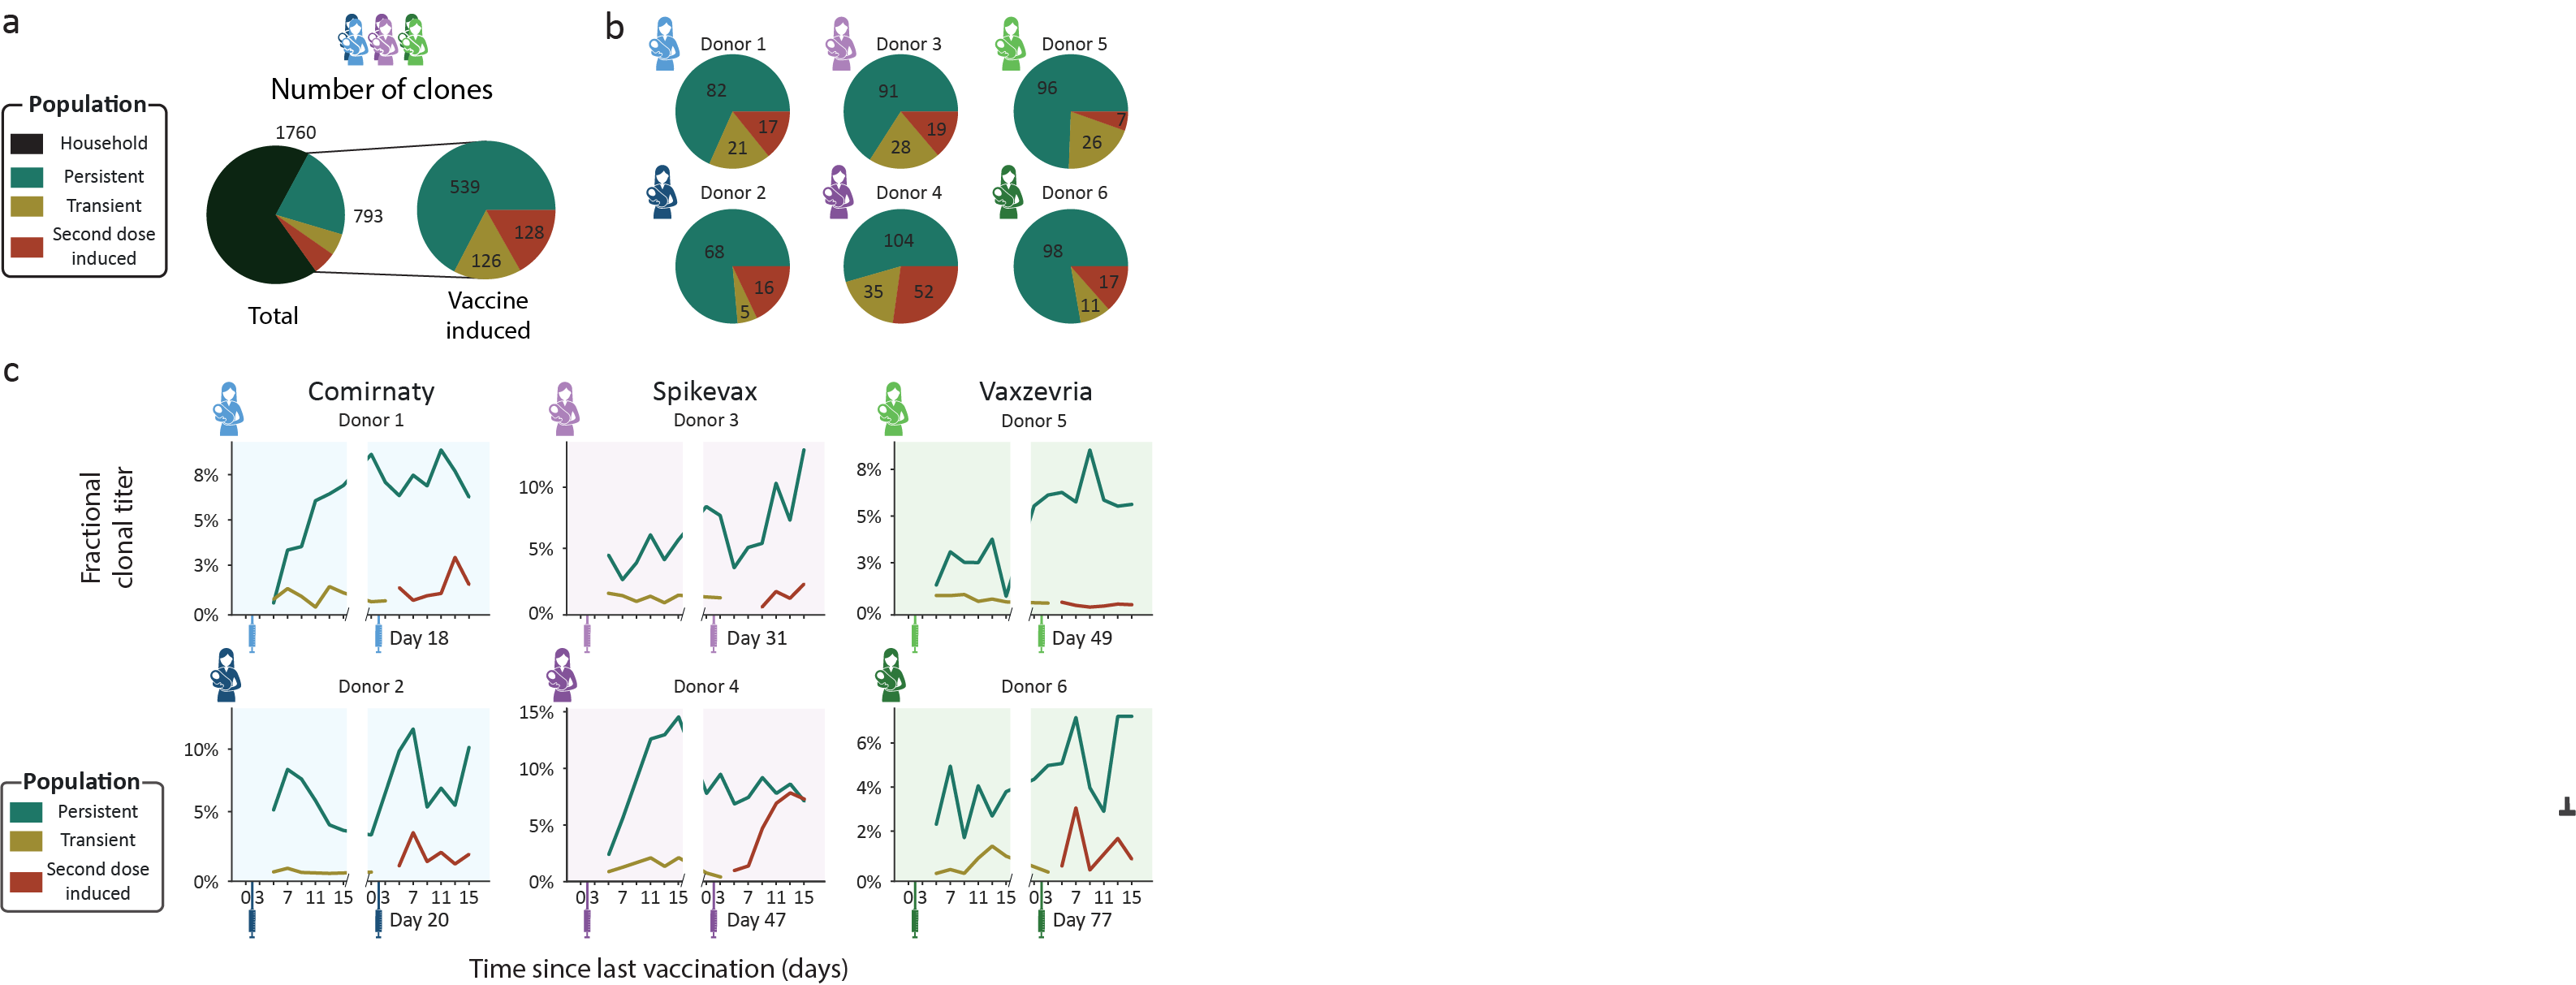
\includegraphics[]{Chapter.4/Figures/f3.png}
  \caption{\textbf{Clonal population analysis.} ~~a) Pie charts showing the total number of unique clones in each population. Clones were assigned to populations based on their detection window relative to the vaccination moments: persistent (teal), transient (mustard), and second dose induced clones (maroon). ~~b) Pie charts showing the number of unique clones in each population per donor. Each pie chart shows data for a single donor (Comirnaty (2 blue donors), Spikevax (2 purple donors) and Vaxzevria (2 green donors)). ~~c) Longitudinal changes in fractional clonal titer (i.e., fraction of the total clonal titer made up by each population) for the vaccine induced clonal populations. Vaccination moments are depicted as color-coded syringes. Each panel shows donor-specific, fractional clonal titers for the three vaccine induced populations. While all donors show a unique repertoire without overlapping clones, varying in number of clones and total clonal titer, when grouped into populations the responses are more consistent. Persistent clones make up the bulk of the vaccine induced SIgA1 clonal titer at nearly every timepoint. The clonal titers of the transient and second dose induced populations account for a much smaller fraction of SIgA1.}
  \label{fig:fig4.3}
\end{figure*}


\subsection{Clonal titer fluctuations can be driven by highly divergent clonal populations}
From the ELISA analysis by Juncker et al. \cite{juncker2022comparing}, donor 4 was identified as the strongest responder in terms of spike-specific IgA. This prompted us to have a closer look at this donor. Our analysis confirmed the strong response, as the vaccine induced clonal titer reached a peak concentration of 26.3 μg/mL, higher than any other donor (maximum 14.7 μg/mL, \textbf{\autoref{fig:fig4.2}c}), and featured 191 unique clones, more than any other donor (maximum 138 clones, \textbf{\autoref{fig:fig4.2}a}).
Uniquely in donor 4, we observed that the second dose induced clonal titer increased comparably to the persistent clonal titer (\textbf{\autoref{fig:fig4.3}c}), indicating that the clonal makeup of the response to the second vaccination was strongly divergent from the response to the initial vaccination. Despite looking very similar to the first phase of the biphasic response (\textbf{\autoref{fig:fig4.2}c}), the second phase of the response was largely driven by the second dose induced population and not the persistent population that was induced by the first dose as the persistent population clonal titer remained relatively stable (\textbf{\autoref{fig:fig4.3}c}). The second dose induced population that drives this second peak in the vaccine induced titer is the largest and most abundant in this study, consisting of 52 unique clones (\textbf{\autoref{fig:fig4.3}}), peaking at over 10 μg/ml (\textbf{\autoref{fig:figs4.3}}). Additionally, the second dose induced population made up 45-50\% of the vaccine induced clonal titer and 39-44\% of vaccine induced clones during the last 3 timepoints (\textbf{\autoref{fig:fig4.4}}), demonstrating how seemingly similar titer fluctuations can be driven by highly divergent clonal populations.
\begin{figure*}[!htb]
  \center
  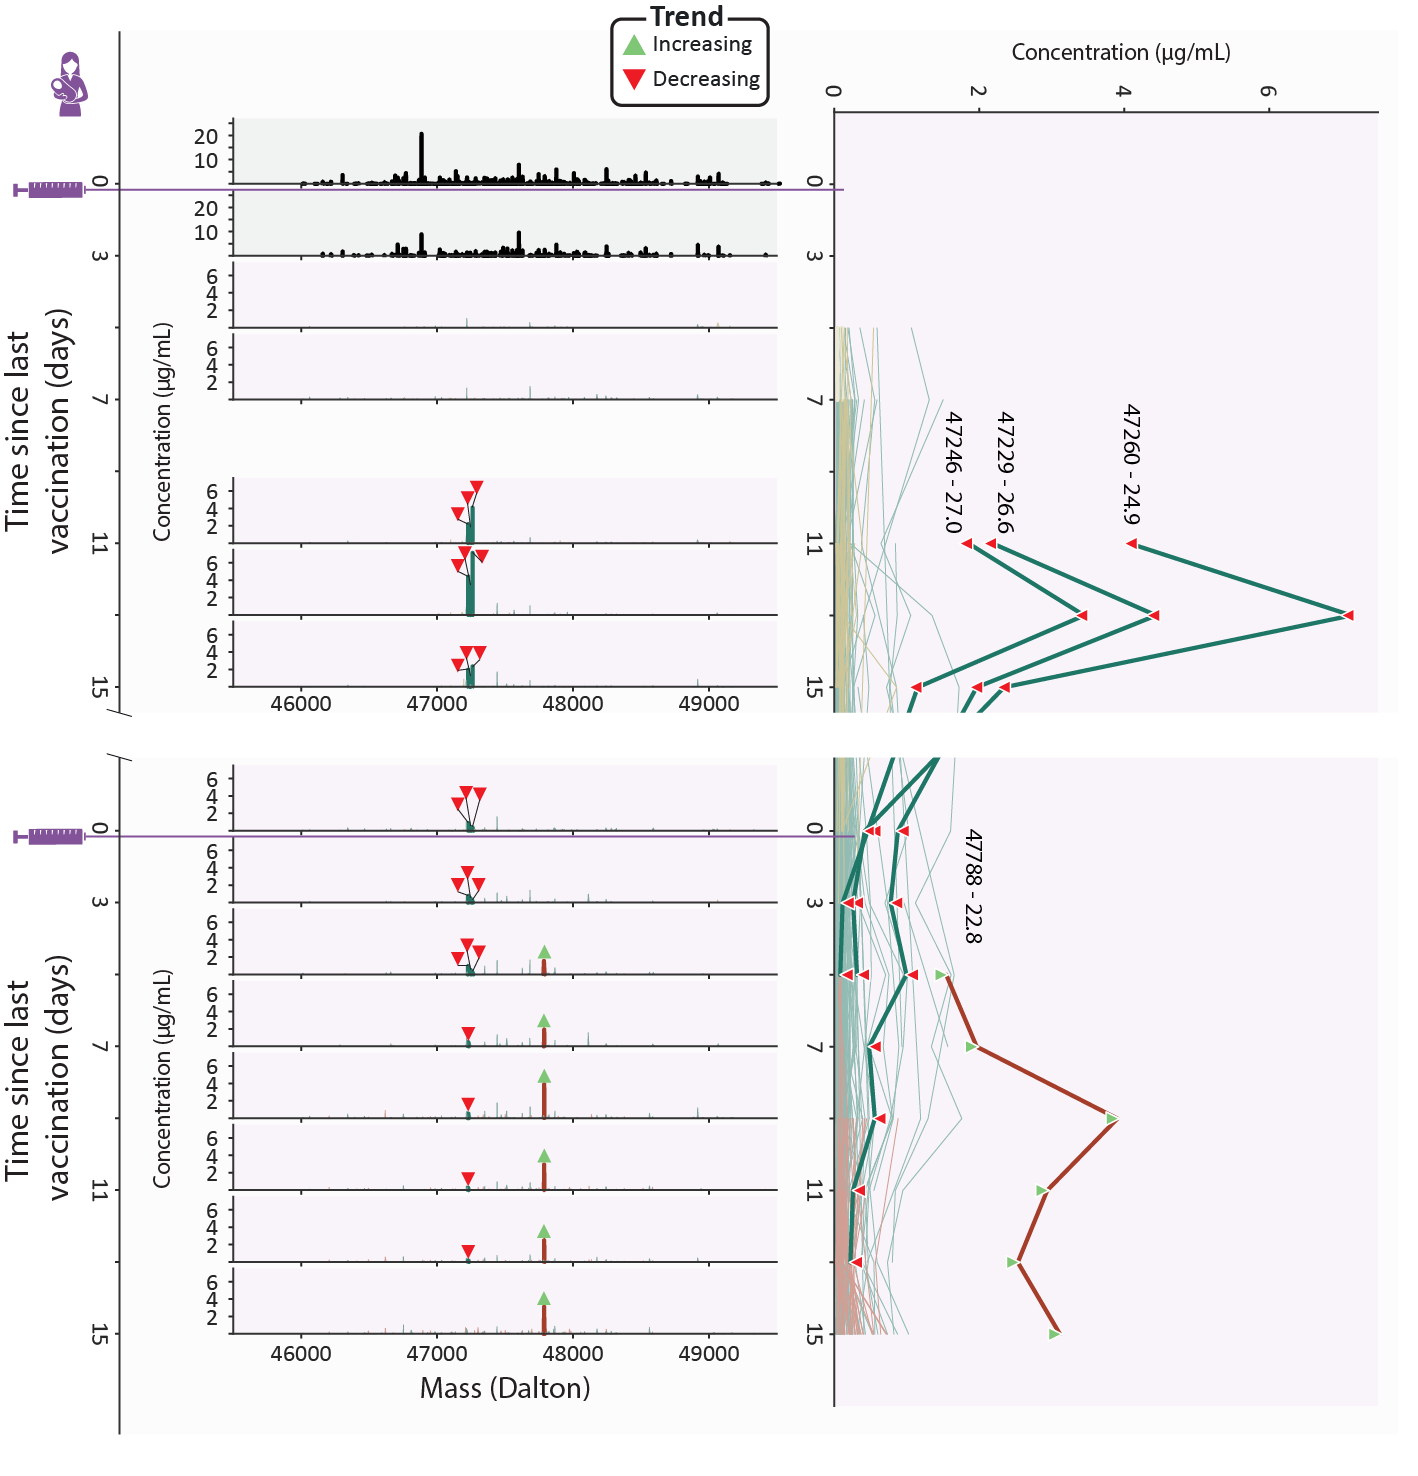
\includegraphics[]{Chapter.4/Figures/f4.png}
  \caption{\textbf{Clonal profile analysis for donor 4, a strong responder.} Changes in the vaccine induced clonal profile for donor 4 are depicted, with the 4 most abundant vaccine induced clones annotated by their mass and retention time, highlighted in bold, with each timepoint annotated with a triangle indicating if the clone trends upwards or downwards in concentration over the course of this study. On the left we show mass profiles (SIgA1 clonal concentration in µg/mL) showing either household clones (top two profiles, in black) or vaccine induced clones (subsequent profiles, with individual clones colored according to their assigned population (persistent (teal), transient (mustard), and second dose induced clones (maroon)). Each peak indicates a single clone and each row a single timepoint. The line plot on the right shows the abundance of individual vaccine induced SIgA1 clones over all timepoints, colored by their population, with the same clones as the mass plots highlighted in bold, labeled with their mass and retention times and annotated with triangles indicating if the clone trends upwards or downwards in concentration throughout the study duration. The highlighted persistent clones are initially highly abundant, but their abundance decreases rapidly, and at the final timepoint none of them are detected. The highlighted second dose induced clone is part of a large and abundant population of second dose induced clones, which at the final timepoints make up 45-50\% of the vaccine induced clonal titer.}
  \label{fig:fig4.4}
\end{figure*}
At these final timepoints, the persistent clonal titer had decreased to approximately half its peak value (\textbf{\autoref{fig:figs4.3}}). However, we did not observe a similar decrease in the number of detected persistent clones suggesting either a simultaneous drop in the intensity of the individual persistent clones or a strong decrease in abundance of one or more dominant clones from this population. Inspection of the individual persistent clones revealed that at its peak (V1D13), the persistent population included three highly abundant clones which together made up 60\% of the persistent clonal titer (\textbf{\autoref{fig:fig4.4}}). While initially these highly abundant clones almost completely dictated the persistent clonal titer fluctuations, they quickly declined in abundance after an initial peak and eventually disappeared while the persistent clonal titer remained relatively stable (\textbf{\autoref{fig:fig4.4}} and \textbf{\autoref{fig:figs4.2}}), seemingly causing the persistent clonal titer drop between the first and second phase.
A similarly dominant second dose induced clone was observed to increase in concentration as the three dominant persistent clones were decreasing at V2D5 (\textbf{\autoref{fig:fig4.4}}). The abundance profile of this clone mirrored the upward trending second dose induced titer (\textbf{\autoref{fig:figs4.3}}) and was the most abundant clone at the final timepoint, at 3.1 μg/mL (\textbf{\autoref{fig:fig4.4}}). However, 37 other second dose induced clones are still detected at the last timepoint and as we saw with the persistent clones, it may be these lower abundant clones that persist in the long term.
These dominant clones demonstrate how clonal titers fluctuations can be strongly influenced by a limited number of abundant clones. Sometimes these clones only amplify the behavior of their parent population, as with the highlighted second dose induced clone. However, they may paint a misleading picture by masking the cumulative behavior of the remaining, lower abundant, clones in the population. The clonal resolution of the LC-MS based Fab profiling method enables us to zoom in on individual clones and allows us to confirm the presence or absence of factors that drive polyclonal responses.

\section{Discussion}
The current body of knowledge about humoral immunity in response to infections and vaccinations are normally determined by ELISAs for total antigen-specific antibody titers and more recently by screening for antigen-specific B-cells. However, recent work by Wolf et al. \cite{wolf2022antibody} shows that the antibody titers are poor markers of the frequency of memory B cells after an infection. Therefore, alternative analyses are needed to assess the basics of humoral immunity. We may gain new insights by uncovering when, how and why specific antibodies come up after an infection or vaccination. A first step in doing this is by monitoring individual clones and extracting patterns from clonal populations, as we demonstrate here.
In this study, we detected a heterogeneous polyclonal response to vaccination, as distinct populations of novel clones emerged in every donor after vaccination. We defined three populations vaccine induced clones can be assigned to based on their window of detection relative to vaccination: transient, persistent and second dose induced clones (\textbf{\autoref{fig:fig4.1}c,} \textbf{\autoref{fig:figs4.2}}). These populations were not only observed in all donors, but also behaved remarkably similar relative to each other, as the persistent population was dominant both in terms of clonal titer and size, regardless of which vaccine the donor had received.
As the donors in this study had not been exposed to SARS-CoV-2 prior to vaccination, the clonal response to the first vaccination can be considered the primary response: a first generation of antibodies, having undergone little to no somatic hypermutation \cite{charlesajaneway2001immunological}. The dominant persistent clones we observe might be the effective portion of the primary response, which are encoded in long lived plasmablasts or memory B cells that proliferate quickly in response to restimulation with the same antigen whereas the transient population could be the ineffective portion of the primary response.
The response to the second vaccination can then be considered the secondary response. In every donor, we observed a population of novel clones emerge during this secondary response. In at least one donor, donor 4, the secondary response had a strongly divergent clonal makeup from the primary response, as it was not predominantly driven by clones induced upon the first vaccine dose but largely by a completely novel clonal population. These novel clones may be the result of a completely new gene recombination but could also be the result of somatic hypermutation of transient or persistent clones, as even small mutations are likely to cause shifts in mass and retention time. Alternatively, they could be clones that escaped detection during the primary response or clones that were derived from previously undetected clones through somatic hypermutation or isotype switching, as our profiling method in this study was limited to SIgA1. While more extensive sequence information is needed to definitively determine the genetic and cellular origin of circulating clones, the second dose induced clones in this study seemingly did not emerge faster than the transient clones, possibly indicating they are not maturations of the first batch of B cells. However, given the small sample size in this study, we are unable to sufficiently answer these questions.
In the parent study of this cohort, spike specific IgAs were longitudinally monitored by ELISA. A biphasic antibody response to SARS-CoV-2 vaccination was observed for spike-specific IgA in these samples, with an accelerated response after the second vaccination, in line with expectations based on leading theories on humoral immune responses \cite{charlesajaneway2001immunological}. We were able to confirm a number of these findings from our case series analysis of this cohort. From both the ELISA and Fab profiling data, donor 4 could be identified as a strong responder, with an observed biphasic response irrespective of analysis type. These confirmations, however, could only be made qualitatively. Quantitatively, we observed a discrepancy between the reported ELISA and measured clonal titers. We believe there are several factors contributing to these discrepancies. First, the applied ELISA measured IgA1 and IgA2, whereas our profiling method detect only IgA1 \cite{keulen2021human, juncker2022comparing}. Furthermore, the ELISA measured spike-specific IgA titers, using a pre-fusion stabilized variant of the spike protein sequence termed 2P \cite{hwang2020cryo-em}. Thus, clones that do not bind to the 2P spike protein variant, but perhaps to other components of the vaccine, will not be detected. Similarly, weak binders may be underrepresented in affinity-based assays. As a recent study showed that low rather than high affinity antibodies delivered greater antibody-mediated receptor activity through increased receptor clustering \cite{yu2023reducing}, these low affinity clones may be of particular importance.
To date, it is often thought that highly efficient neutralizing antibodies would perhaps not be among the most abundant clones. However, at the current stage of implementation the most reliable detection and quantitation through LC-MS is limited to relatively abundant clones, and low abundant clones likely exist at concentrations below our limit of detection. One way to study these low abundant clones is through fractionation or purification. While there is value in retaining biological context by minimizing purification, simultaneous analysis of the sample in an enriched form can enable a more targeted look at clones of interest or provide us with contextual information about clones in our sample such as binding affinity. For example, in a recent study van Rijswijck et al. \cite{rijswijck2022discriminating} analyzed serum samples of SARS-CoV-2 patients, with and without affinity purification, and combined the results to yield information about the cross-reactivity of individual clones to different SARS-CoV-2 variants of concern. This illustrates how the ability to identify and track clones between samples and experiments can be used to obtain functional information about individual clones, and how we can relate this information back to the original abundance profile. Future applications of LC-MS fab profiling hold the promise of high throughput characterization of antibody repertoires, allowing for a greater understanding of the mechanisms related to antibody mediated immunity and defining immune signatures that predict how an individual will respond to future encounters with similar antigens. We imagine this to have future applications similar to HLA phenotypes for organ transplants or genetic markers for cancer treatment. In addition to defining such “biomarkers” for individual patients, we could identify markers of efficacy for individual clones, potentially enabling the direct identification of potential therapeutic antibodies from polyclonal samples. We believe studies like this pave the way to elucidate the mechanisms involved in mounting an effective antibody response and can lead to future targeted efforts to find potential therapeutic candidates.


\section{Methods}

\subsection{Study design}
In this study we used samples from an existing prospective longitudinal study COVID MILK – POWER MILK \cite{juncker2022comparing}. All participants were subjected to longitudinal analysis of specific antibodies against the SARS-CoV-2 spike-protein by ELISA and general SIgA1 Fab clonal profiling in human milk after vaccination against COVID-19 with BNT162b2/Comirnaty developed by Pfizer-BioNTech, mRNA-1273/Spikevax developed by Moderna or AZD1222/Vaxzevria developed by Oxford/AstraZeneca. Ethical approval was acquired from an Independent Ethics Committee\\
(2020.425/NL74752.029.20). The study was conducted in accordance with the principles of the declaration of Helsinki and the ICH GCP Guidelines, and the Regulation on Medical Research involving Human subjects.

\subsection{Subjects}
Details concerning subjects have been extensively described \cite{juncker2022comparing}. Briefly, lactating women in the Netherlands receiving one of the above-described SARS-CoV-2 vaccines were eligible to participate and were recruited through social media platforms. There were no exclusion criteria. All participants were requested to send their vaccination certificate, including the type of vaccination and lot number. From the larger study a subset of 2 women per vaccine group were selected based on the following criteria: 1) a pre-vaccine milk sample was available, 2) data from an enzyme-linked immunosorbent assay (ELISA) with the SARS-CoV-2 spike protein for human milk SIgA was available and indicated high spike-specific SIgA titers. Written informed consent was obtained from all participants.

\subsection{Sample collection}
Sample collection was performed between January 2021 and July 2021. Human milk samples were collected longitudinally over a period of up to 95 days (\textbf{\autoref{fig:fig4.1}}). In this study, 16 samples of human milk were analyzed per lactating woman. These samples were collected according to the following schedule: one sample before the first vaccination and one sample on days 3, 5, 7, 9, 11, 13, and 15 after the first vaccination. This schedule was the same for the second vaccination (\textbf{\autoref{tab:tabs4.1}}). Participants were instructed to empty one breast in the morning, before the first feeding moment, and collect 5 mL of milk after mixing the milk. Participants were requested to store the milk samples in the home freezer. Samples were transported back to the lab on dry ice and remained at -80 until analysis \cite{juncker2022comparing, keulen2021human}.

\subsection{Fab clonal profiling from human serum and milk}

\subsubsection{IgA enrichment, capture, and digestion}
Methods for IgA1 Fab profiling have previously been extensively detailed \cite{bondt2021human, bondt2021direct}. Briefly, all IgA was captured using CaptureSelect IgA affinity matrix (Thermo Fisher Scientific). Human milk samples were assumed to contain 0.8 µg/µL SIgA and added to excess amount of bead slurry, PBS, and 200 ng of the monoclonals anti-CD20 mIgA1 (7D8-IgA1) and anti-cMET (5D5v2-IgA1). These monoclonals were used as internal standards for quantification, and were a gift from Genmab (Utrecht, NL). Samples were incubated followed by removal of the flow through, containing all non-IgA human milk components. The samples were then washed several times and IgA was digested overnight with the O-glycopeptidase from Akkermansia muciniphila, OgpA (OpeRATOR®, Genovis, Llund, Sweden). Digestion was performed using 40 U SialEXO (a sialidase cocktail to remove sialic acids from the O-glycans) and 40 U of OgpA enzyme, and incubated overnight at 37 °C, in an Eppendorf thermal shaker (Eppendorf, The Netherlands). Following overnight digestion with OgpA, Ni-NTA agarose slurry was added to the samples to bind the enzyme and incubated for 30 min. Finally, the flowthrough, containing the IgA1 Fabs, was collected by centrifugation.


\subsubsection{Fab profiling by LC-MS}
The LC-MS and data processing approaches as described by Bondt et al. were applied \cite{bondt2021human, bondt2021direct}. In short, the collected Fab samples were separated by reversed phase liquid chromatography on a Thermo Scientific Vanquish Flex UHPLC instrument, equipped with a 1 mm x 150 mm MAbPac analytical column, directly coupled to an Orbitrap Fusion Lumos Tribrid mass spectrometer (Thermo Fisher Scientific, San Jose, California, USA). The column preheater and the analytical column chamber were heated to 80°C during chromatographic separation. Fab samples were injected as 10 µL and subsequently separated over a 62 min gradient at a flow rate of 150 µL/min. The gradient elution was achieved using mobile phases A (0.1\% HCOOH in Milli-Q HOH) and B (0.1\% HCOOH in CH3CN), see previous publications for details \cite{bondt2021human, bondt2021direct}. The instrument was operating in Intact Protein and “Low Pressure” mode for the acquisition of MS data, with a spray voltage of 3.5 kV set from minute 2 to minute 50 of the gradient. The ion transfer tube temperature was set at 350°C, vaporizer temperature at 100°C, sheath gas flow at 15, auxiliary gas flow at 5, and source-induced dissociation (SID) was set at 15 V. Spectra were recorded with a resolution setting of 7,500 (@ 200 \emph{m/z}) in MS1. Scans were acquired in the range of 500-4,000 \emph{m/z} with an AGC target of 250\% and a maximum injection time set to 50 ms. For each scan 5 µscans were recorded.

\subsubsection{IgA1 clonal profiling data analysis}
Intact masses were retrieved from the generated RAW files using BioPharmaFinder 3.2 (Thermo Scientific). Deconvolution was performed using the ReSpect algorithm between 5 and 57 min using 0.1 or 0.3 min sliding windows with a 25\% offset, a merge tolerance of 30 ppm, and noise rejection set to 95\%. The output mass range was set from 10,000 to 100,000 with a target mass of 48,000 and mass tolerance 30 ppm. Charge states between 10 and 60 were included and the Intact Protein peak model was selected.
Further data analysis was performed using Python 3.9.13 (with libraries: Pandas 1.4.4 \cite{mckinney2010data}, NumPy 1.21.5 \cite{walt2011numpy}, SciPy 1.9.1 \cite{virtanen2020scipy}, Matplotlib 3.5.2 \cite{hunter2007matplotlib:} and Seaborn 0.11.2). Masses of the BioPharmaFinder identifications (components) were recalculated using an intensity weighted mean considering only the most intense peaks comprising 90\% of the total intensity. Using the mAb standards, the intensity was normalized, a relative mass shift was applied to minimize the mass error and a retention time shift was applied to minimize deviation between runs.
Components between 45 and 53 kDa with the most intense charge state above \emph{m/z} 1000 and a score of at least 40 were considered Fab portions of IgA1 clones. The clones in samples of the same donor were matched between runs using average linkage (unweighted pair group method with arithmetic mean UPGMA) L∞ distance hierarchical clustering. Flat clusters were formed based on a cophenetic distance constraint derived from a mass and retention time tolerance which were 2 Da and 1 min respectively. Clones within a flat cluster were considered identical between runs. Clones that were only detected at a single timepoint within a donor were excluded from the analysis. Clones were assigned to populations according to their detection window relative to vaccination as outlined in \textbf{\autoref{fig:figs4.2}}.

\section{Acknowledgements}
We would like to sincerely thank all the mothers who participated and all students and research assistants who helped with this study.

\subsection{Data Availability}
The mass spectrometry proteomics data have been deposited to the MassIVE repository with the dataset identifier MSV000092157.


\subsection{Trial registration}
This research project was registered at the Dutch Trial Register on May 1st, 2020, number: NL 8575, URL: https://onderzoekmetmensen.nl/nl/trial/23001.


\subsection{Funding statement}
This research received funding through the Netherlands Organization for Scientific Research (NWO) TTW project 15575 (SCdG and AJRH), the ENPPS.LIFT.019.001 project (AJRH) and the Roadmap Program X-omics 184.034.019 (AJRH). This research received further support by Stichting Steun Emma Kinderziekenhuis. MJvG acknowledges the Amsterdam Infection and Immunity Institute for funding this work through the COVID-19 grant (24175). KAD acknowledges the Amsterdam Reproduction and Development Institute for funding this work though the AR\&D grant (V.000296).

\subsection{Declaration of Interests}
JBvG is the founder and director of the Dutch National Human Milk Bank and a member of the National Health Council. JBvG has been a member of the National Breastfeeding Council from March 2010 to March 2020.


\section{Author Contributions}
KAD, JBvG and AJRH conceived the ideas and jointly designed the study and experiments. KAD, MH, DMHvR, MJAD and AB performed all experiments. SCdG performed the data analysis. HGJ, SJM, BJvK and JBvG collected all samples. SCdG, KAD, AB and AJRH wrote the manuscript, all others provided edits. AJRH and JBvG provided resources and funding for the project. All authors contributed to the article and approved the submitted version.


\clearpage
\begin{subappendices}
  \beginsupplement

  \section{Supplementary material}
  \begin{figure*}[!htb]
    \center
    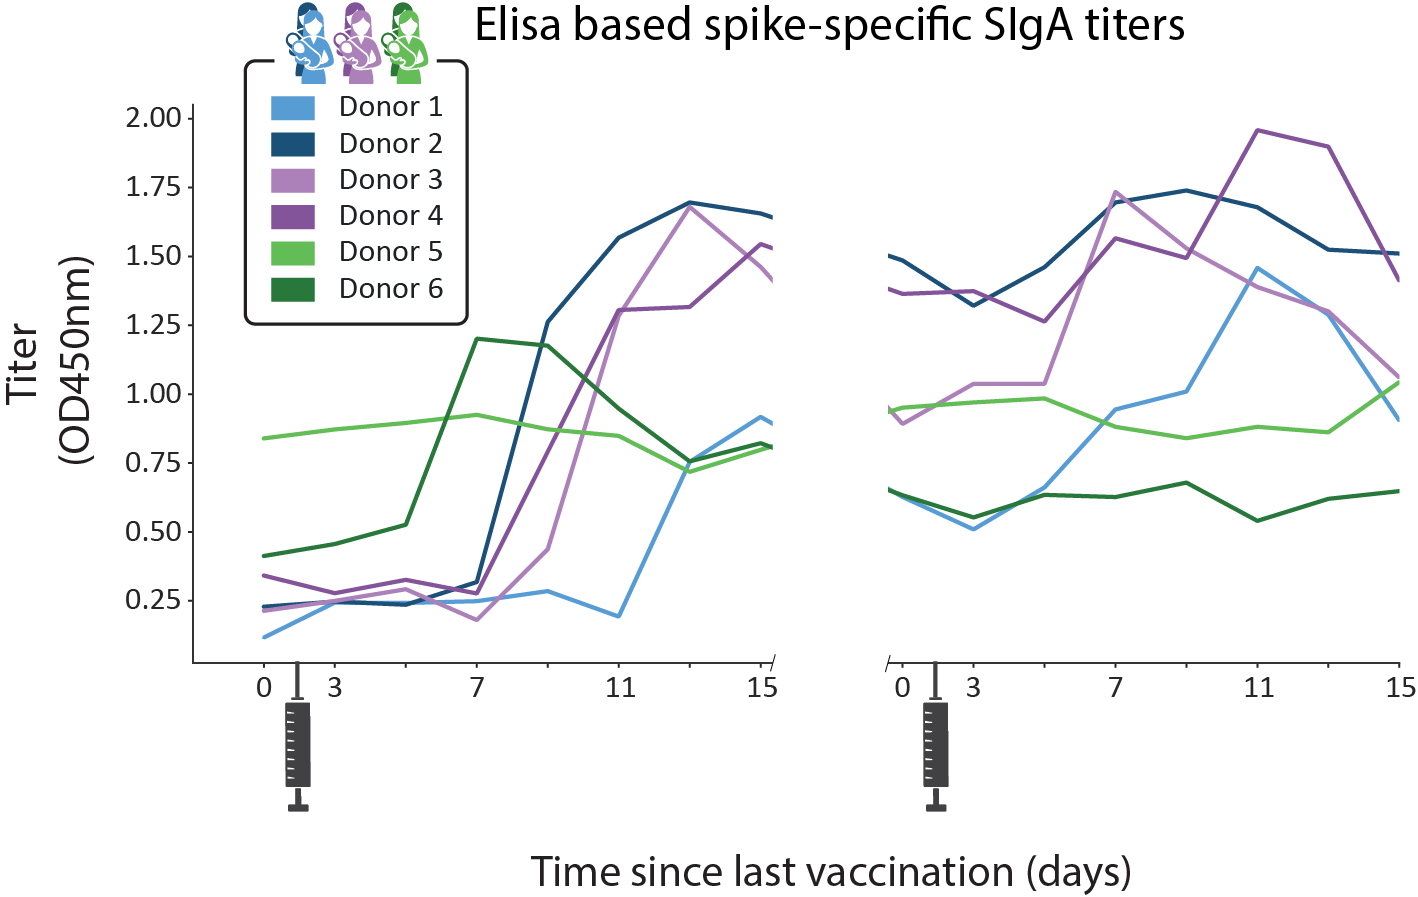
\includegraphics[]{Chapter.4/Figures/fs1.png}
    \caption{\textbf{Quantified ELISA Spike-specific IgA titers.} A biphasic antibody response to SARS-CoV-2 vaccination was observed for spike-specific IgA, with an accelerated response after the second vaccination. Original data from Juncker et al. \cite{juncker2022comparing}.}
    \label{fig:figs4.1}
  \end{figure*}
  \begin{figure*}[!htb]
    \center
    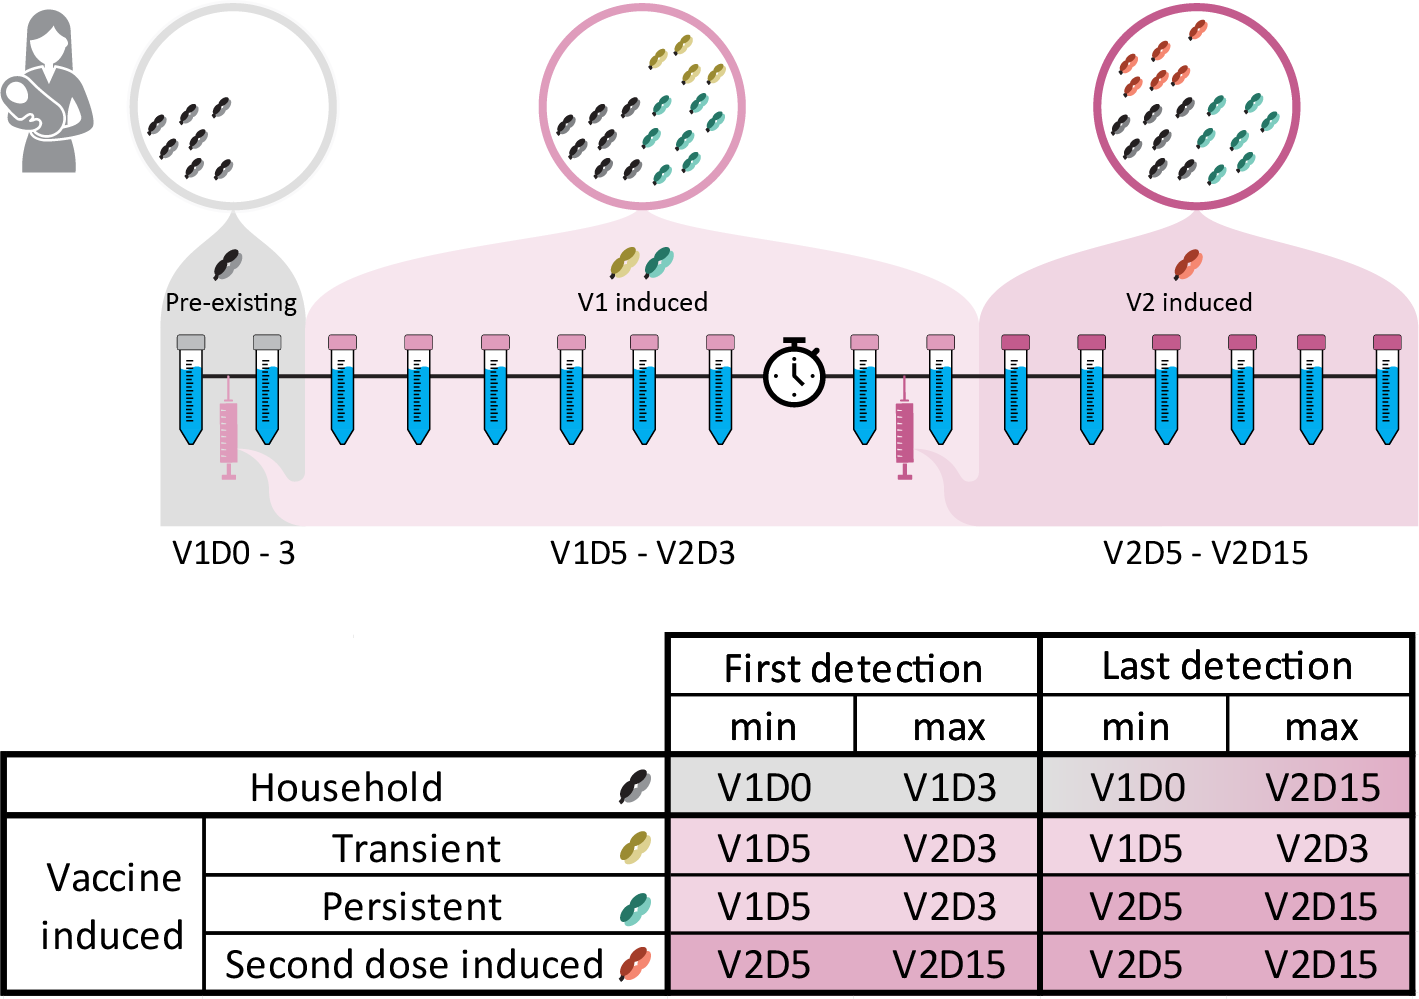
\includegraphics[]{Chapter.4/Figures/fs2.png}
    \caption{\textbf{Clonal population inclusion criteria.} Description of the criteria used to assign clones to the designated clonal populations based on their first and last detection moment (i.e., their detection window) relative to vaccination. Time windows are colored by appearance of clones relative to vaccination. Grey window (V1D0 – V1D3): Not attributed to vaccination. Light pink window (V1D5 – V2D3): Attributed to the first vaccination. Dark pink window (V2D5 – V2D15): Attributed to the second vaccination. Clones not detected in the first window were considered vaccine induced clones, and further assigned as follows: Clones first detected in the light pink window were considered transient clones if they were only detected in the light pink window, or persistent clones if they were detected in the dark pink window as well. Clones first detected in the dark pink window were considered second dose induced clones.}
    \label{fig:figs4.2}
  \end{figure*}
  \begin{figure*}[!htb]
    \center
    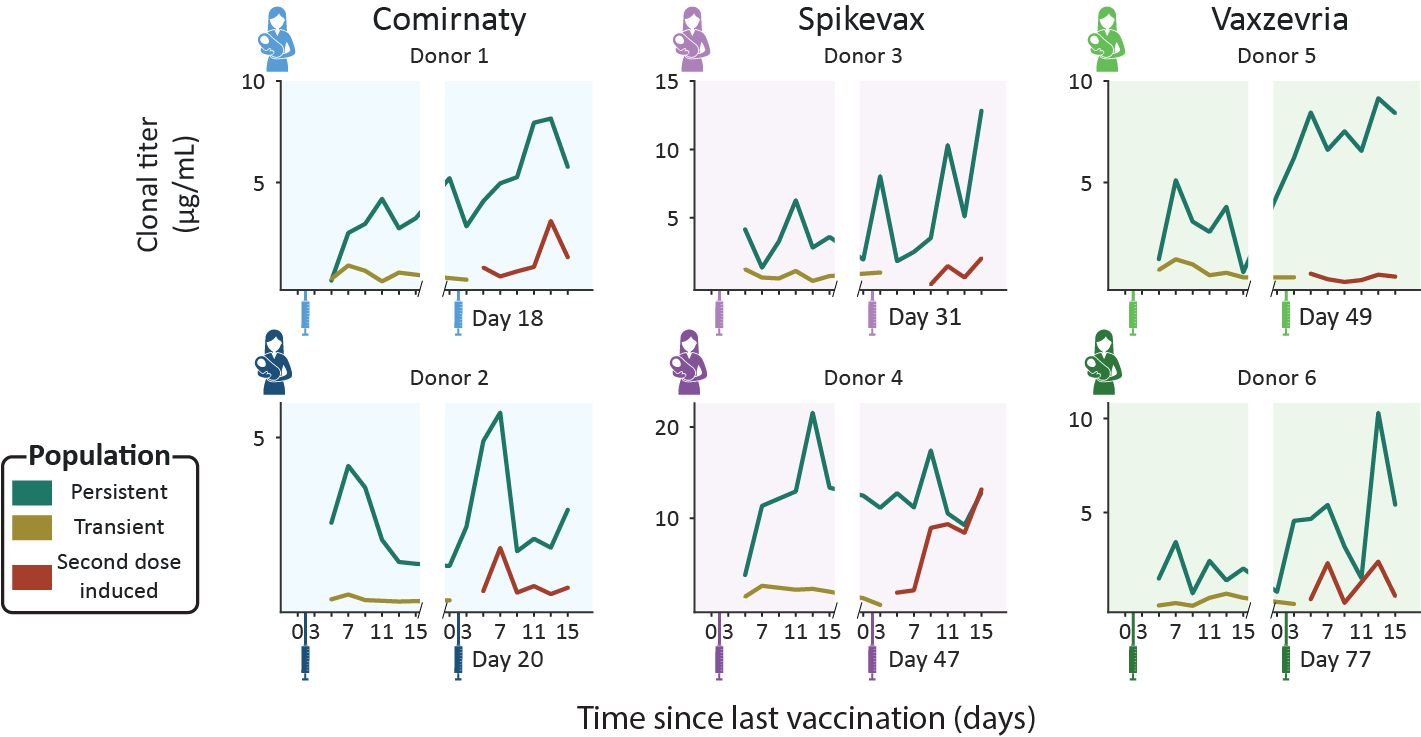
\includegraphics[]{Chapter.4/Figures/fs3.png}
    \caption{\textbf{Longitudinal changes in absolute clonal titers for the vaccine induced populations.} Each panel shows the population clonal titer (i.e., the summed concentrations of the individual SIgA1 clones) for our three assigned, vaccine induced populations: Persistent clones (teal), transient (mustard) and second dose induced (maroon). Each panel shows data for a single donor (Comirnaty (2 blue donors), Spikevax (2 purple donors) and Vaxzevria (2 green donors)). Vaccination moments are depicted as color-coded syringes. Each panel shows donor-specific, clonal titers for the three vaccine induced populations. While all donors show a unique repertoire without overlapping clones, varying in number of clones and total clonal titer, when grouped into populations the responses are more consistent. Persistent clones make up the bulk of the vaccine induced SIgA1 clonal titer at nearly every timepoint. The clonal titers of the transient and second dose induced populations account for a much smaller fraction of SIgA1.}
    \label{fig:figs4.3}
  \end{figure*}
  \begin{table*}[!hbt]
    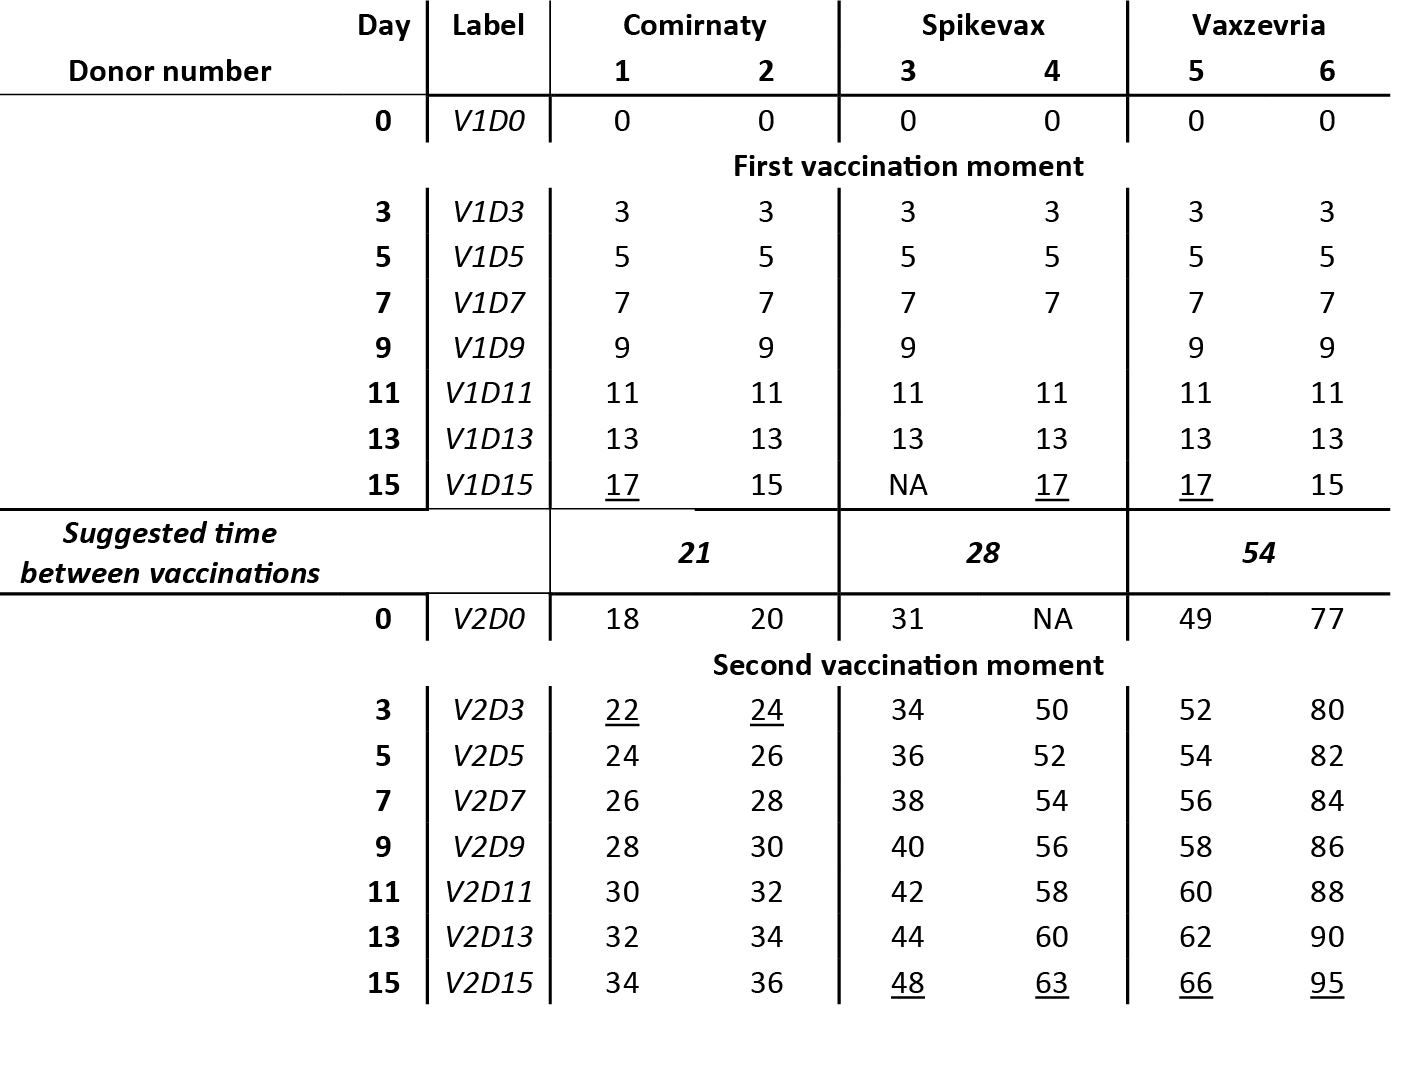
\includegraphics[]{Chapter.4/Figures/ts1.png}
    \caption{
      \textbf{Sampling schedule for each donor.} The “Day” column indicates the number of days between the last vaccination and the collection of each sample. The “Label” column indicates the label that is to refer to each sample in this manuscript. These are constructed as follows: for a sample labeled V1D3, D3 indicates the number of days since the last vaccination and V1 indicates the last vaccination received by the donor, so this sample was taken three days after the first vaccination. Samples collected just before vaccination are referred to as day 0 (i.e., V1D0 and V2D0). The actual days samples were collected from each individual donor are indicated as the number of days between the first vaccination and each sample collection. For some samples, the number of days between sample collection and the preceding sample collection deviated slightly from the schedule, these samples were underlined. NA indicates that the sample was collected but a date was not recorded. Blank spaces indicate that no sample was collected. The parent study included a follow-up sample, V2D70, for donor 2, 3 and 4. For donor 4, sample V2D15 was lost, and the follow-up sample was used instead. To unify the number of samples analyzed per donor per population, we excluded the remaining 2 follow-up samples from our analysis. The original study refers to donor 1-6 as PM2272, PM2183, PM2387, PM0281, PM0287 and PM0267 respectively.
    }
    \label{tab:tabs4.1}
  \end{table*}

\end{subappendices}

\clearpage
\section*{References}
\bibliographystyle{Stylesettings/pnas}
\patchcmd{\thebibliography}
{\clubpenalty 4000\widowpenalty 4000}
{\clubpenalties 1 10000 \widowpenalties 1 10000}
{}{}
\bibliography{chapmerge}
\stopthumb



\picturechapter{Modular antibody \emph{de novo} sequence analysis using multi-tier LC-MS/MS data}{Chaptercovers/ch5.pdf} \label{ch-5}
\vspace*{0.25cm}

{\footnotesize Sebastiaan C. de Graaf, Douwe Schulte, A. Bondt, Max Hoek, Weiwei Peng, Sem Tamara, Joost Snijder, Richard A. Scheltema, Albert J.R. Heck}
%%
\begin{center}
  \vspace{3cm}
  \includegraphics[]{Chapter.5/Figures/Ch5.png}
  \vspace{0.25cm}
\end{center}

\begin{flushleft}
  \vspace*{\fill}
  \rule{\textwidth}{1pt}\\[0cm]
\end{flushleft}

\begin{abstract102}
  Antibodies form an important class of biomolecules that are produced by the immune system to defend us against infections. Their importance is underlined by their successful use as therapeutic agents, enabled by their production as recombinant monoclonal proteins (mAbs). Prior to development of an antibody lead, identification of the amino acid sequence needs to be achieved. Commonly B-cell sequencing is used to identify the DNA/RNA sequences that lead to the antibodies of interest, although only a small subset of the B cells produce antibodies that end up in circulation. More recently mass spectrometry-based (MS) methods have been used for sequencing, with the added benefit that this is a direct approach to extract the sequence of the protein in circulation, thereby potentially providing insights into post-translational modifications. Both approaches have their implicit challenges, and the complete extraction of the amino acid sequence is still difficult to achieve. In MS-based approaches mostly shotgun proteomics has been applied, where the antibody is digested into peptides prior to identification. With such an approach, gaps in sequence coverage often arise, mostly in the complementarity-determining regions (CDRs) of the antibody that are responsible for the recognition and binding of infectious agents. Here, we demonstrate that by combining shotgun proteomics with middle-down (MD) proteomics, where the protein or large fragments thereof are measured intact, these gaps can be filled and better information on the sequence can be extracted. We therefore developed and described here software solutions to iteratively integrate data from BU and MD proteomics.
\end{abstract102}
\thumbforchapter

\section{Introduction}
\lettrine[lraise=0.1, nindent=0em, slope=-.5em]{A}{ntibodies}, or immunoglobulins, are one of the cornerstones of the human immune system and are abundantly present in various bodily fluids, such as serum, saliva, milk, the lumen of the gut, and cerebrospinal fluid \cite{schroeder2010structure}. Because of their important role in combatting infectious diseases, immunoglobulins have been intensively studied and in the last decades have taken centre stage for the development of novel therapeutics \cite{kaplon2021antibodies, marks2020how, raybould2020thera-sabdab:}. In the last decade, antibodies have become the best-selling drugs in the market, notably in 2018 eight of the top ten bestselling drugs were biologics.
New antibody leads for biotherapeutics can be extracted from various sources, such as immunized animals or recovered patients who carry pathogen neutralizing antibodies \cite{bornholdt2016isolation, corti2016protective, valgardsdottir2021identification}. The incredible potential for diversity of immunoglobulin molecules in the human body, with over 10\textsuperscript{15} theoretically possible sequences \cite{schroederjr.2006similarity, briney2019commonality}, indicates that each antigen exposure may lead to a unique, personalized (polyclonal) antibody response. One way to chart the antibody repertoire is to sequence the B-cell receptors of all B cells that can produce antibodies. It is however thought that only a marginal fraction of all these B cells indeed produce immunoglobulin proteins that end up in circulation, making this an inefficient undertaking. Alternatively and more ideal, investigation and sequencing of antibodies occurs directly at the protein level \cite{hom2022exploring}.
Mass spectrometry (MS) has become the method of choice for analysing protein mixtures \cite{altelaar2013next-generation, aebersold2016mass-spectrometric}, but sequencing polyclonal antibody mixtures still poses one of the major remaining challenges \cite{sen2017automated, peng2021mass, srzentić2020interlaboratory}. Most protein analyses by MS are performed by peptide-centric proteomics, also called shotgun or bottom-up (BU) proteomics, where the presence and relative abundance of proteins is inferred from peptides obtained by digesting the proteins with proteases, prior to sequencing. For the identification, this approach makes use of a protein sequence database to generate theoretical peptides from which the expected precursor mass and fragmentation spectrum is generated \cite{aebersold2003mass}. A sequence database is however not available for the full repertoire of antibodies, as their sequences are the result of the recombination and mutation of several genes encoded by many different alleles in each person. An option to sequence antibodies by shotgun proteomics is by using \emph{de novo} sequence analysis, where peptide sequences are directly determined from the fragmentation spectra. The resulting short peptide \emph{reads}, typically 5-25 amino acid residues in length, are assembled into longer \emph{contigs} or even full-length \emph{protein chain} sequences \cite{sen2017automated, tran2016complete, guthals2012shotgun}. A factor that makes read assembly for antibodies particularly difficult is that the sequence of both the light- and heavy chain of an antibody are made up of alternatingly conserved and hypervariable sequence domains \cite{charlesajaneway2001generation, alberts2002generation}. Fortunately, the quality of software platforms for \emph{de novo} sequence analysis of antibodies by MS is steadily increasing \cite{graaf2022perspective}. Virtually all published platforms make use of homologous sequence templates \cite{sen2017automated, tran2016complete, schulte2022template-based, castellana2010template}, obtained by comparing experimental data to an immunogenetic database such as the IMGT \cite{lefranc2003imgt, lefranc2020immunoglobulins}. The commercially available antibody sequencing platform Supernovo for example takes BU data as an input and returns a full-length sequence, along with the determined germline template sequences \cite{sen2017automated}. Through recent development in software and mass spectrometry results of these approaches may now lead to correct sequencing, albeit only for monoclonal antibody samples \cite{peng2021mass}. However, established software solutions in the field, including Supernovo, cannot yet sequence antibodies in polyclonal mixtures with equal success.
Recent advances in instrumentation, separation, sample preparation and computational power have facilitated protein-centric proteomics (also called top-down proteomics). This enables the simultaneous analysis of an entire protein, removing the need for protein inference \cite{toby2016progress}. This approach is very enticing as it side-steps the need for assembling peptide sequences into a full protein sequence. While the field has not yet matured to yield spectra that can routinely be used for confident \emph{de novo} sequencing without additional data, the continuous advances indicate that the future of antibody sequence analysis will surely include these techniques as a complementary source of information to the more established peptide-centric (BU) analyses. One particularly striking example of this is the use of middle-down (MD) proteomics for antibody sequence analysis, which improves sequence coverage and reduces complexity of the spectra by cleaving the constant region of the heavy chain with high specificity \cite{johansson2008ides:}. Reports of sequencing components of polyclonal mixtures are currently released as proof-of-concept studies \cite{bondt2021human, dupré2021de, schulte2022template-based}, where most of the studies make use of some form of intact protein (fragment) analysis, pointing towards integrative workflows combining multiple MS approaches as the way forward.
Recently, a tool to sequence polyclonal mixtures using only BU \emph{de novo} peptides was reported. The tool, named Stitch, yields exciting results by resequencing an abundant clone from serum \cite{schulte2022template-based}. Here we describe an integrated approach that builds upon Stitch by integrating MD-MS data, with the aim of improved antibody sequencing. This workflow sequences a target chain, selected from deconvoluted MS1 spectra of reduced antibody chains, in a modular, three-stage process based on germline domains as defined in the IMGT residue numbering scheme \cite{lefranc1997unique}. Each stage deals with increasingly large sequence segments, first sequencing the framework regions (FRs), then CDRs with flanking FRs (FR-CDR-FRs), and ultimately full-chain sequences (\textbf{\autoref{fig:fig5.1}a}). To demonstrate the performance of this approach, we analysed three samples of increasing complexity: a pure therapeutic antibody, namely Trastuzumab, both in a monoclonal sample and in a mixture of three monoclonal antibodies, as well as a single abundant IgA1 clone endogenously present in the serum repertoire of a sepsis patient. We used these samples to test the effectiveness of the workflow, by reconstructing the known sequence of the Trastuzumab heavy chain to a high degree in the monoclonal sample as well as in the more complex mixture of three monoclonal antibodies. We next applied the approach to sequence an abundant IgA1 heavy chain in a highly diverse polyclonal sample of IgA1 clones present in the serum of a sepsis patient. We chose to describe our sequencing efforts for the more complex heavy chain rather than describe the same steps for the light chain simultaneously, for the sake of brevity as the analysis treats the two as completely separate entities. We show how integration of MD-MS data can be used to resolve ambiguity in \emph{de novo} sequence predictions, particularly in hypervariable regions, through determining the mass of the CDR and using this mass to filter candidate CDR sequences and confirm their pairing to the fragmented precursor chain. We hypothesize that such improvements will be particularly beneficial when analysing polyclonal mixtures of increasing complexity or when lower sample amounts are available. The algorithms supporting the analyses were programmed in the C\# programming language and are freely available on GitHub.

\section{Results}
Antibody sequencing by any source of information poses a tough challenge due to the hypervariable yet homologous nature of the vast number of sequences. For example, reference databases are of little to no benefit when sequencing the hypervariable CDRs, which in turn makes assigning bottom-up reads to these regions extremely difficult. Using MD proteomics provides not yet a realistic alternative, as the fragment coverage in MD-MS, although superior to that of top-down (TD) MS, is still too limited for stand-alone \emph{de novo} sequencing, although exciting progress is made for sequencing reduced light chains \cite{dupré2021de, melani2019direct}. Here, our hypothesis was that by combining BU- with MD-MS data, and reference sequences from immunological databases, these sources of information can complement each other and be used to fill gaps not covered by the individual approaches. Therefore, we make use of MD-MS fragmentation spectra combined with the relatively conserved nature of the FRs to determine the molecular mass of the CDRs. This is subsequently used as a filter to substantially reduce the number of candidate CDR sequences while simultaneously confirming their pairing to the fragmented precursor target chain.
The workflow consists of three stages: we first consider only FR sequences, then the FR-CDR-FR sequences, and finally the full-length sequences. Each stage first generates a candidate pool of sequence-solutions by considering ambiguities left by the previous stage, then evaluates these candidates using the integrated evidence streams, and finally resolves the ambiguities by discarding candidates that do not have supporting evidence (\textbf{\autoref{fig:fig5.1}a}). By starting with the FRs, which are relatively well-conserved sequence segments, and resolving ambiguities at this scale before moving to longer, more variable segments by joining adjacent FR candidates into FR-CDR-FR contigs, the size of the search space at each stage remains at manageable sizes, limiting computational costs and enabling the analysis of more complex samples (\textbf{\autoref{fig:fig5.1}b}).
\begin{figure*}[!htb]
  \center
  \includegraphics[]{Chapter.5/Figures/f1.png}
  \caption{\textbf{Modular sequencing can be used to limit the search space.} ~~a) Schematic of data-integration workflow. The approach consists of three stages in which increasingly large sequence segments are sequenced and then used as input for the next stage. Initially, only the framework regions (FRs) are sequenced. Then the FR candidates are converted into extended FR-CDR-FR candidates (\emph{i.e.}, CDRs with adjacent FRs). Finally, the FR-CDR-FRs are recombined into full chain candidates. Each stage follows a flow starting with sequence candidate generation based on input data (“Generate”). These candidates are scored using multiple data streams (“Integrate”), then the best candidates are selected using these scores (“Evaluate”). ~~b) Size of the search space throughout the workflow. The approximate number of candidates is shown in the modular approach (pink) versus processing the whole sequence at once (teal). By first sequencing smaller segments, the search space can be kept relatively small. The segment candidate pool is expanded at the start of the stage and reduced after scoring. This ensures we never consider more than $\sim$10\textsuperscript{3} segment candidates at the same time, keeping computational cost in balance .}
  \label{fig:fig5.1}
\end{figure*}


\subsection{Target mass determination and sample characterization by using MD-MS}
\label{ch:mass-determ}
To characterize the complexity of the samples and determine the precursor masses of the target chains, we collected MD LC-MS/MS data for all samples. Our MD approach was performed according to previously published protocols (see \textbf{\autoref{ch:ig-capt}: Immunoglobulin capture and Fab generation}) \cite{bondt2021direct, bondt2021human}. These protocols yield Fab fragments by specifically cleaving the Fc portion of the heavy chain. The resulting Fab fragments were then reduced before LC-MS/MS analysis, to yield separated Lc and Fd chains. We then deconvoluted the MS1 spectra to assess the number of unique Lc and Fd masses in each sample (\textbf{\autoref{fig:fig5.2}})
\begin{figure*}[!htb]
  \center
  \includegraphics[]{Chapter.5/Figures/f2.png}
  \caption{\textbf{Increasing complexity leads to an increase in ambiguity in mass determination in middle-down proteomics of antibodies.} LC-trace (top panel), zero-charge deconvoluted mass spectrum (middle panel), and averaged MS2 spectrum (bottom panel). ~~a) Pure Trastuzumab with clear signals for the light chain and the Fd chain. ~~b) Mixture of Trastuzumab and two other monoclonal antibodies. ~~c) Polyclonal sample from plasma. The contributions of the target and paired chains diminish relatively when the background becomes more complex.}
  \label{fig:fig5.2}
\end{figure*}

For the monoclonal sample, as expected, 2 highly abundant peaks were observed (originating from the separated Lc and Fd chains), accounting for over half of the total deconvoluted intensity. When adjacent peaks in both mass and retention time (±50 Da and ±1 minute) are considered, this increases to over 90\% with the remaining masses consisting of background peaks of less than 5\% relative abundance (\textbf{\autoref{fig:fig5.2}a}). For the mixture of 3 mAbs, likewise and as expected, six abundant peaks were observed. The abundance of the target chains (±50 Da and ±1 minute) made up $\sim$33\% of the deconvoluted intensity. The other clones make up a total of 50\% of deconvoluted intensity and $\sim$20\% is background (\textbf{\autoref{fig:fig5.2}b}). Lastly, for the polyclonal sample, the target clone (±50 Da and ±1 minute) made up less than 20\% of deconvoluted intensity (\textbf{\autoref{fig:fig5.2}c}). The data in \textbf{\autoref{fig:fig5.2}} highlight challenges in deconvoluting MD-MS spectra. We observe that the deconvolution software reports (inaccurate) masses  besides the expected masses, increasingly so for more complex samples. To obtain the most exact masses, we averaged the MS1 spectra recorded over the elution window of each target chain (\textbf{\autoref{fig:fig5.2}}; highlighted in red) before deconvolution. This improved the mass assignments to within 30 ppm accuracy for the Trastuzumab Fd in the monoclonal and mix sample and yielded a target precursor mass of 24811.17 Da for the most abundant clone in the polyclonal sample extracted from serum. Similarly, the MS2 fragmentation spectra were averaged over the elution windows of the target chains and deconvoluted. This yielded 919, 265 and 469 deconvoluted fragment ion peaks for the monoclonal, mix and polyclonal sample respectively (\textbf{\autoref{tab:tabs5.1}}  ).


\subsection{Using multi-enzyme shotgun proteomics data for \emph{de novo} sequencing}
\label{ch:bu-ms}
As part of the analysis each sample was also measured by BU-MS, by digesting each sample with 4 proteases in parallel and collecting peptide-centric LC-MS/MS data. The resulting spectra were submitted for \emph{de novo} peptide identification using PEAKS \cite{ma2003peaks:}, yielding a total (\emph{i.e.}, cumulatively from all protease treatments) of 14000, 27421 and 35003 \emph{de novo} peptide reads for the monoclonal sample, the mixture of three, and the polyclonal sample, respectively (\textbf{\autoref{tab:tabs5.1}}). To illustrate the growing challenges of sequencing through shotgun proteomics in more complex samples, we reconstructed the known sequence of the Trastuzumab Fd from the \emph{recombinant benchmark samples} (\emph{i.e.}, the monoclonal and mixture of three sample) using BU-MS data alone. To this end, the peptide reads for these samples were submitted to the \emph{de novo} peptide assembly tool Stitch \cite{schulte2022template-based}. The resulting output for the monoclonal sample was nearly perfect (\textbf{\autoref{fig:fig5.3}a}). However, the consensus sequence as obtained for the sample from the mixture of 3 mAbs contained 4 erroneous residue predictions in the FR2, and 6 in the CDR1 and CDR2 (\textbf{\autoref{fig:fig5.3}c}). These errors were the result of low peptide coverage, caused by assigning reads to the wrong templates. This caused splitting of reads that belonged to the same chain. Furthermore, the unassisted germline recombination by Stitch failed to select the correct V-region for recombination, as it was not the highest scoring V-region in the mix sample. This standard \emph{de novo} sequencing of a recombinant mAb, already becomes difficult when two other mAbs of equal abundance are spiked into the sample.
\begin{figure*}[!htb]
  \center
  \includegraphics[]{Chapter.5/Figures/f3.png}
  \caption{\textbf{Sequencing higher complexity samples lead to a loss of fidelity in sequencing when using only shotgun proteomics data.} Sequencing results for the monoclonal (panel a-b) and mixture of 3 mAbs (panel c-d) samples are shown. Each sample was submitted to Stitch twice: as a \emph{template selection} run (light blue, panel a and c) and a \emph{definitive} run (dark blue, panel b and d). Each panel shows residue candidates as letters and depth of coverage as bars. The monoclonal sample had no coverage below the cut-off (pink highlight), very few erroneous residue candidates (grey residues), ambiguity, or errors in the consensus sequence (marked with “\emph{x}”). The mixture of 3 mAbs sample had substantially more stretches of sequence with low coverage (pink bars), resulting in more ambiguity, erroneous candidates, and errors.}
  \label{fig:fig5.3}
\end{figure*}

To tackle these issues, we ran Stitch again with refined templates (\emph{i.e.} the consensus sequence as output by the initial Stitch run, or \emph{template selection} run, rather than the germline sequence) and a lower score cut-off for the input reads (50 instead of 85). To ensure recombination of the correct V-region, we manually defined which V-region templates should be recombined by Stitch by providing refined templates equal to the number of abundant clones present in the MD data (1 and 3 for the monoclonal and mixture sample, respectively; \textbf{\autoref{fig:fig5.2}a and b}). For the monoclonal sample we selected the best scoring V-region, IGHV3-66, as a refined template. For the sample of 3 mAbs we selected 3 V-region templates: the highest unique score (IGHV4-39), the highest score (IGHV4-30-4), and the highest score in a different family (IGHV3-66). This additional Stitch run, or \emph{definitive} run, gave a major improvement for analysis of Trastuzumab in the 3 mAb sample, as it improved the depth of coverage 2 to 28-fold and raised depth of coverage above the dynamic cut-off (the depth of coverage at Cys104, \textbf{\autoref{fig:fig5.3}}) for 13 out of 21 positions (\textbf{\autoref{fig:fig5.3}d}). Pleasingly, these adjusted settings had no detrimental effects on the performance for the monoclonal sample (\textbf{\autoref{fig:fig5.3}b}), although some ambiguity remained in the predicted sequence for Trastuzumab in the 3 mAb sample.


\subsection{Integrating multiple evidence streams}

\subsubsection{Performance on recombinant samples}

\paragraph{Framework region sequencing}
\label{ch:fr}
Using the residue frequency tables (\textbf{\autoref{fig:figs5.1}}) from both Stitch runs, as well as a residue frequency table generated from the IMGT database, FR candidate sequences were generated by converting ambiguous residues into sequence candidates (\textbf{\autoref{fig:figs5.1}}). This yielded between 1 and 756 candidates per target FR (\textbf{\autoref{tab:tabs5.2}}) and included the known correct candidate for all recombinant benchmark samples. These candidates were evaluated against experimental BU- and MD-MS evidence and ranked by a combination of the resulting scores. For BU-MS scoring, a score was used that represents the depth of coverage of exact sequence matches longer than 6 residues, weighted by match length (termed Shotgun-score; \textbf{\autoref{tab:tabs5.3}}). For MD-MS scoring, a score was used that represents the overlap between theoretical fragments of the sequence and peaks in the MD fragmentation spectrum (MD-score; \textbf{\autoref{tab:tabs5.3}}). The MD-score is obtained using a \emph{sliding window} scoring algorithm, which slides theoretical fragments generated from a given (sub)sequence over the spectrum to find the best scoring position, and thus outputs the optimal prefix- and suffix- mass of a given contig (\textbf{\autoref{fig:figs5.2}}). Candidates missing highly conserved residues (Cys23, Cys104) as well as terminal segment (\emph{i.e.}, FR1 and FR4) candidates with illogical prefix- or suffix- masses were removed in a first pass filtering step. This reduced the candidate lists up to 10-fold, to a maximum of 90 candidates (\textbf{\autoref{fig:figs5.3}}).
We further filtered the candidate pools to a maximum of 40 candidates (\textbf{\autoref{tab:tabs5.2}}) without eliminating any correct candidates by manual inspection of the scores. For the monoclonal sample, the correct FR1 candidate was ranked \#1 with a large discrepancy between scores (\textbf{\autoref{fig:figs5.3}}). As FR2, FR3, and FR4 only had one candidate each, no selection was needed. However, it was encouraging to see that the sliding window algorithm was able to correctly determine the prefix masses for these contigs with a mass error that did not exceed 18 ppm.
The candidate pools for the mixture of 3 mAbs were reduced from 240, 756, 5 and 4 candidates to 40, 7, 1 and 2 candidates for al FRs respectively (\textbf{\autoref{tab:tabs5.2}}). For FR1, we rejected 200 candidates in the first pass, leaving 40 candidates. No further filtering was possible, as fragment and read coverages were too low for confident filtering (maximum of 2 fragments and no read coverage past Cys23). The FR2 candidates had many overlapping scores (\textbf{\autoref{fig:figs5.3}}) due to low read coverage of the N-terminal ambiguous residues (\textbf{\autoref{fig:fig5.3}c and d}) and a near total overlap of theoretical fragments for these candidates. We rejected the lower MD-scores (106 vs 121), which represented the same fragments but without a fragment match on the second residue. This reduced the number of candidates from 756 to 90. Subsequent filtering using the Shotgun-score, rejecting all but the best Shotgun-score (9.4k), left only 7 candidates, representing a single remaining ambiguous N-terminal residue. For FR3, only 1 out of 5 candidates had the highly conserved Cys104, leading us to reject all other candidates. For FR4, we rejected all candidates not starting with the conserved Trp118 but considered the difference in Shotgun-score for the remaining 2 candidates too small to reject either.

\paragraph{Complementarity determining region sequencing}
\label{ch:cdr}
To determine the sequence of the CDRs, we extended the selected FR candidates into FR-CDR-FR candidates. All adjacent FR candidates were paired to obtain all possible neighbouring pairs. We then calculated the mass gap between each of these FR pairs (which is equal to the theoretical molecular weight of the CDR sequence) using the prefix- and suffix- mass of each FR candidate. Each FR pair was converted into a set of FR-CDR-FR candidates by connecting the FRs with candidate CDR sequences. These candidate CDR sequences were generated by first connecting peptide reads that extend from the FRs into the CDR, then discarding the candidates that do not match the calculated molecular weight of the CDR at 5 Da tolerance (\textbf{\autoref{fig:figs5.4}}). The resulting FR-CDR-FR candidates were scored and ranked using the MD- and Shotgun- score (\textbf{\autoref{tab:tabs5.3}}).
The top 10 FR-CDR-FR candidates for each FR pair were manually evaluated based on the scores to select the most likely FR-CDR-FR candidates. For both recombinant benchmark samples, these candidates contained the correct sequence for CDR1, CDR2 and CDR3. For the monoclonal sample, 10 FR-CDR-FR candidates were generated per CDR (\textbf{\autoref{tab:tabs5.2}}). The correct candidate for each CDR could easily be selected using the Spectrum and Shotgun-score (\textbf{\autoref{fig:figs5.2}}). The selected candidates all had the top MD-score (255, 508 and 1561 for the CDR1, CDR2 and CDR3 respectively) and the best (CDR1 and CDR2) or second best (CDR3) Shotgun-score (137k, 56k and 122k respectively).
For the mixture of 3 mAb sample 1106, 49 and 20 FR-CDR-FR candidates were generated for the CDR1, CDR2 and CDR3, respectively (\textbf{\autoref{tab:tabs5.2}}). Despite the much larger starting pools, the correct CDR1- and CDR2- candidates could be selected unambiguously during manual inspection as they had the second best and best MD-scores (143 and 257 for CDR1 and CDR2 respectively) and the top Shotgun-score (30k and 40k respectively; \textbf{\autoref{fig:figs5.3}}). The selected FR-CDR-FR candidates for CDR1 also caused rejection of the remaining incorrect FR1 and FR2 candidates, which left only 7 FR-CDR-FR candidates for CDR2 as the rest did not contain the right FR2.
Scoring for the CDR3 was more ambiguous. Fragment coverage was insufficient to make a distinction between the FR-CDR-FR candidates, as MD-scores ranged only from 280 to 282. The Shotgun-scores were distributed in two clusters based on which FR4 candidate was included (\textbf{\autoref{fig:figs5.3}}). The correct FR4 (starting with WGQGT) scored $\sim$221k while the incorrect FR4 (starting with WGQGS) scored higher ($\sim$244k). However, we noted that the candidates with the wrong FR4 lacked connecting reads between the FR4 and CDR3. The candidates with the correct FR4 sequence had fewer but longer and more overlapping reads which connected the CDR3 and FR4 better (average read length of $\sim$25 vs average read length of $\sim$12). We rejected the higher Shotgun-scores on this basis.
The candidate pool with the correct FR4 included 2 incorrect FR-CDR-FR candidates, SR\textbf{\emph{WNDG}}FYAMDY and SR\textbf{\emph{DNWG}}FYAMDY, that were nearly identical to the correct candidate, SR\textbf{\emph{WGGDG}}FYAMDY. We selected these 3 candidates based on the presence of longer and more overlapping reads in the CDR3 than the other 7, same as above. However, we could not discriminate between the 3 isobaric candidates at this point, leaving 3 candidates for the CDR3.


\paragraph{Full chain sequencing}
We next expanded the scope to the entire target chain to verify the selected FR-CDR-FR candidates. To achieve this, we recombined all remaining FR1 to FR4 candidates and transformed these FR-sets into full length chain candidates by joining the FRs with CDR candidates in the same manner as before (see \textbf{\autoref{ch:cdr}: Complementarity determining region sequencing}; \textbf{\autoref{fig:figs5.4}}). The resulting chain candidates that deviated more than 5 Da from the precursor mass in the MD-MS data were discarded. To ensure that the selected FR-CDR-FR candidates indeed represented the best predictions, all resulting chain candidates were scored and ranked using the MD- and Shotgun- score (\textbf{\autoref{fig:figs5.3}}).
This recombination yielded 930 chain candidates for the monoclonal sample and 616 for the mixture of 3 mAb sample. The correct chain candidate for the monoclonal sample was ranked \#1, despite not having the highest Shotgun-score (267k vs 270k) or MD-score (1815 vs 1818). For the mixture of 3 mAb sample, the chain candidates made up solely out of previously selected FR-CDR-FR candidates were ranked \#3-5, with the correct sequence at \#5. The top 2 candidates had CDR3 sequences that were previously rejected in the CDR sequencing stage, which were again rejected on the same basis (shorter, less overlapping reads). The isobaric CDR3s still could not be confidently ranked as the scores were too close, with Shotgun-scores between 255.7k and 255.8k and MD-scores between 426.1 and 427.2 (\textbf{\autoref{fig:figs5.3}}). Low fragment coverage combined with other clones being present at similar concentrations seemingly prevented us from resolving the final ambiguities for the mix sample. This is highlighted by the large difference between the MD-scores for the correct chain candidates (426 for the mix sample vs 1815 for the monoclonal sample).


\subsubsection{Performance on the complex polyclonal samples}
After successfully reconstructing the known sequence of Trastuzumab from the recombinant samples, we proceeded to analyse the polyclonal sample. We selected the most abundant heavy chain (precursor mass 24811.17 Da; \textbf{\autoref{tab:tabs5.1}}) as a sequencing target and prepared deconvoluted fragmentation spectra from the raw MD-MS data (see \textbf{\autoref{ch:mass-determ}: Target mass determination and sample characterization using MD-MS}; \textbf{\autoref{fig:fig5.2}c}). To generate FR candidates for the selected target chain, we submitted \emph{de novo} peptide reads to Stitch (see \textbf{\autoref{ch:bu-ms}: Using multi-enzyme shotgun proteomics data for \emph{de novo} sequencing}). From the \emph{template selection} run we selected IGHV3-33, the most abundant V-region in the Stitch results, for recombination during the \emph{definitive} run (\textbf{\autoref{fig:fig5.4}a}). The Stitch frequency tables from both runs were then converted into FR candidates as described above (see \textbf{\autoref{ch:fr}: Framework region sequencing}; \textbf{\autoref{fig:figs5.1}}).
\begin{figure*}[!htb]
  \center
  \includegraphics[]{Chapter.5/Figures/f4.png}
  \caption{\textbf{Sequencing an abundant IgA1 heavy chain in a polyclonal sample converges on a single sequence prediction.} The sequencing process of the target chain in the polyclonal sample is shown. Residue candidates per position are shown in sequence logos, with rejected residue candidates in grey. Below the sequence logos the number of candidates at the start and end of the stage is shown. ~~a) The selected germline template, IGHV3-33*06, is shown along with the deviations from the final sequence. ~~b) In the FR sequencing stage, we reduced all FR candidate pools to 4 candidates or less despite starting with large pools of FR3 and FR4 candidates. ~~c) During the CDR sequencing stage, we converged on a single CDR1 and CDR2 candidate, thereby also rejecting the remaining incorrect FR1 and FR3 candidates. The only remaining ambiguity was in between two isobaric CDR3 sequences. ~~d) Recombining the remaining FR candidates into chain sequences yielded 975 chain candidates. Two of these contained the previously selected CDRs. These two candidates were isobaric, had highly similar Shotgun-scores and fully overlapping fragment coverage. ~~e) middle-down fragment coverage for the final sequence (constant region not shown).}
  \label{fig:fig5.4}
\end{figure*}

FR candidate generation yielded 8, 2, 384 and 64 candidates for the FR1 to FR4 respectively. After scoring and filtering this was reduced to 2, 1, 3 and 4 candidates (\textbf{\autoref{fig:fig5.4}b}, \textbf{\autoref{tab:tabs5.2}}). From the FR candidates which remained after the first pass (see \textbf{\autoref{ch:fr}: Framework region sequencing}; \textbf{\autoref{tab:tabs5.2}}), we rejected all but the top scoring candidates with respect to MD-score (10, 155, 163 and 133 for FR1 to FR4 respectively; \textbf{\autoref{fig:figs5.3}}). We then manually selected candidates for each FR based on Shotgun-score. For FR1, we selected the top 2 candidates (34k and 35k Shotgun-score) as the other two candidates had an LTC motif that had a lower Shotgun-score. This left a single ambiguous isobaric residue, an N-terminal pyro-Q/E. For FR2, only 1 candidate had the top MD-score, which was much higher than the alternative candidate (155 vs 105). For FR3 the top 3 Shotgun-score candidates were selected (27k-30k), leaving 2 ambiguous sites (Q/E and TV/RA, \textbf{\autoref{fig:fig5.4}b}). For FR4, the top 4 candidates in terms of Shotgun-score (308k-310k) were selected, representing a single ambiguous N-terminal residue (\textbf{\autoref{fig:fig5.4}b}).
Using these FR-candidates, 20, 30 and 120 FR-CDR-FR candidates were generated for CDR1 to CDR3 respectively. The top MD- and Shotgun-scores were unambiguous for CDR1 and CDR2 (\textbf{\autoref{fig:figs5.3}}), identifying the CDR1 as GLTFSTYD (MD-score 118, Shotgun-score 57k), and CDR2 as LWNDGYNK (MD-score 377, Shotgun-score 51k). By selecting these FR-CDR-FR candidates, 2 out of 3 remaining FR3 candidates could be rejected leaving 40 FR-CDR-FR candidates for CDR3. From these, we selected 2 isobaric FR-CDR-FR candidates (\textbf{\emph{LG}}QR\textbf{\emph{PL}} and \textbf{\emph{GL}}QR\textbf{\emph{LP}}) with the top Shotgun-scores (346.2k and 346.4k) and the second-best MD-score (both 370.7) (\textbf{\autoref{fig:fig5.4}c}, \textbf{\autoref{fig:figs5.3}}).
Recombining the selected FR candidates into chain candidates yielded 975 chain candidates. Two chain candidates were made up of previously selected FR-CDR-FR candidates and scored very well as they had the fourth highest MD-score (434) and top Shotgun-scores (411k; \textbf{\autoref{fig:figs5.3}}). To resolve the remaining ambiguity in the CDR3 (\textbf{\autoref{fig:fig5.4}d}), we revisited the peptide coverage for this region. This revealed a break in the peptide coverage of CDR3 in one of the candidates suggesting the CDR3 sequence LGQRPL. However, strong support for the LP motif in the CDR3 led us to reinspect the \emph{de novo} reads manually, where we found several reads suggesting the CDR3 sequence LGQRLP, a sequence absent in any single bridging or overhanging CDR3 reads. Rescoring this sequence indeed revealed an increased Shotgun-score, from 411.3k to 411.7k, providing the final piece of the sequence (\textbf{\autoref{fig:fig5.4}e}).


\section{Discussion}
With this work we show that integration of BU and MD data is beneficial to achieve a higher fidelity for \emph{de novo} extraction of the sequences of antibodies. To provide a solid basis with the \emph{de novo} peptide data, we utilize Stitch \cite{schulte2022template-based} although this step does not yet allow for unambiguous sequence determination. To correct the errors and resolve this ambiguity, MD fragmentation data was used. Although the MD data for even the most abundant clone in a mixture is far from complete, we show that it can be used as a potent filter to remove erroneous candidates and even to assist with filling gaps in the sequence. We have used the presented workflow to simultaneously sequence light and heavy chains, but for the sake of brevity have omitted the light chain sequencing efforts in this manuscript. As we analyse one chain at a time, there is little difference between the analysis of light and heavy chains aside from differences arising from the quality of the data or the complexity of the target. Light chains are less complex owing to a lower degree of somatic hypermutation and the lack of a D-segment. Unsurprisingly therefore, these targets performed equally well or better than their heavy chain counterparts.
The polyclonal sample used in this study still represents a hand picked case for sequencing plasma antibodies, where the sample was dominated by a single clone. While moving to more complex samples will surely pose new challenges, it has been shown that circulating antibody repertoires are, more often than previously thought, dominated by a limited number of clones \cite{bondt2021human, bondt2021direct}. We are therefore optimistic that the presented approach will be applicable to a significant fraction of polyclonal samples . Additionally, for those samples where it does fall short due to sample complexity, enrichment strategies can be applied before analysis in an effort to reduce sample complexity and increase the chance of successfully obtaining the protein sequence. Another point to improve is the need for expert manual interpretation at various points in this workflow, which significantly limits the throughput. Although the main goal of the presented work was to define a broadly applicable protocol for polyclonal antibody sequencing, we have not yet been able to define robust score cut-offs for several decision points making this an intermediate step in the development of a fully automated pipeline. The integration of multiple data sources, as well as the diversity of the analysed samples (polyclonal, complex), targets (light or heavy chain, dominant clones, isotypes and subclasses), regions (FR1-4, CDR1-3) and segments (FRs, FR-CDR-FR, chain), makes this an even bigger challenge. As the field matures however, a point will be reached where scoring functions and corresponding cut-offs can be defined. This will automate an ever-increasing portion of this work, eventually leading to a high throughput, fully automated method.


\section{Materials and Methods}

\subsection{Immunoglobulin capture and Fab generation}
\label{ch:ig-capt}

\subsubsection{Recombinant IgG1 sample preparation}
The IgG purification and generation of IgG1 Fabs for the recombinant monoclonal and mix samples was performed as previously published \cite{bondt2021human}. IgGs were captured using CaptureSelect FcXL affinity matrix (Thermo Scientific). Mobicol spin filters were assembled according to manufacturer instructions and placed in 2 mL Eppendorf tubes. Then 20 µL FcXL affinity matrix slurry was added to the spin filter, followed by three washing steps with 150 µL PBS, in which the liquid was removed by centrifugation for 1 min at 1000 × \emph{g}. Two additional washing steps with 150 µL were performed. The affinity matrix was resuspended in 150 mL PBS, and 100 µg of sample was added. The samples were then incubated while shaking for one hour. Next, the flow-through was collected and the affinity matrix with bound IgGs was washed four times with 150 µL PBS. bound IgGs were digested overnight using 50 µL PBS containing 100 U of the IgdE protease (FabALACTICA®, Genovis, Llund, Sweden) on a thermal shaker (Eppendorf, The Netherlands) at 37 °C. Next, 10 µL of Ni-NTA beads were added to bind and remove the His-tagged protease and left incubating for an additional 30 minutes. The flow through after centrifugation contained the IgG1 Fab fragments generated.

\subsubsection{Serum IgA1 sample preparation}
The IgA purification and generation of IgA1 Fabs for the polyclonal sample was performed as previously published \cite{bondt2021direct}. IgAs were captured from a patient serum sample using CaptureSelect IgA affinity matrix (Thermo Scientific). 40 µL bead slurry was added directly to Pierce spin columns with screw cap (ThermoFisher Scientific). The beads were then repeatedly washed with 150 µL PBS by centrifugation at 500 × g, room temperature (RT). After the third wash, a plug was inserted to the bottom of the individual spin columns and 100 µL PBS was added to the beads. Twenty microliter of serum was diluted in 150 µL PBS and added, then incubated for 1 hour while shaking. Following the incubation, the plugs were removed from the spin columns and the diluted sample was collected by centrifugation for 1 min at 500 × g, RT. Then the beads were washed four times by addition of 200 µL PBS and subsequent centrifugation for 1 min at 500 × g, RT. After the fourth wash the plugs were reinserted into the bottom of the spin columns. We added to each spin column 50 µL PBS containing 40U SialEXO (SialEXO, Genovis, Llund, Sweden), a sialidase cocktail to remove sialic acids from the O-glycans, and incubated for 1 h at 37°C with continuous shaking at 750 rpm. 1 µL (40 U) of OgpA enzyme (OpeRATOR, Genovis, Llund, Sweden) was then added, and incubation was continued overnight, in and Eppendorf thermal shaker. Next, 10 µL of Ni-NTA beads were added to bind and remove the His-tagged proteases and left incubating for an additional 30 minutes. The flow through after centrifugation contained the IgA1 Fab fragments generated.

\subsection{Bottom-up \emph{de novo} sequencing}

\subsubsection{Sample preparation}
Fab fragments were digested for BU analysis as described previously \cite{bondt2021human}. All purified Fab antibody fragments were dried under vacuum and resuspended in a 50 mM aqueous ammonium bicarbonate buffer. For each bottom-up analysis, 12 µg of sample was used, 3 µg per protease. For digestion with trypsin, chymotrypsin, elastase and thermolysin, a sodium deoxycholate (SDC) buffer was added to a total volume of 80 µL, 200 mM Tris pH 8.5, 10 mM TCEP, 2\% (w/v) SDC final concentration. For digestion with pepsin, a urea buffer was added to a total volume of 80 µL, 2M urea, 10 mM TCEP. Samples were denatured for 10 min at 95 °C followed by reduction for 20 min at 37 °C. Next, iodoacetic acid was added to a final concentration of 40 mM and incubated in the dark for 45 min at room temperature for alkylation of free cysteines. Then for trypsin, chymotrypsin and thermolysin, 50 mM ammonium bicarbonate buffer was added to a total volume of 100 µL. For pepsin 1 M HCl was added to a final concentration of 0.04 M. A total of 0.06 µg of each protease was added and the mixture incubated for 4 hours at 37 °C. After digestion 2 µL formic acid was added to precipitate the SDC. SDC was removed by centrifugation for 20 min at maximum speed (20817 × \emph{g}) after which the supernatant was moved to a new tube. The final samples were desalted by Oasis HLB (Oasis).  Sorbent was wetted using 2x 200 µL ACN, followed by equilibration with 2x 200 µL water/10\% formic acid.  The sample was loaded and washed with 2x 200 µL Mili Q water/10\% formic acid.  Finally, the sample was eluted using 2x 50 µL water/50\% ACN/10\% formic acid and dried down by vacuum centrifuge. Prior to MS analysis samples were reconstituted in 2\% FA.

\subsubsection{LC-MS/MS}
Data acquisition was performed on the Orbitrap Fusion Tribrid Mass Spectrometer (Thermo Scientific, San Jose, CA, USA) coupled to UHPLC 1290 system (Agilent Technologies, Santa Clara, CA, USA) as previously published \cite{bondt2021human}. Briefly: Peptides were trapped (Dr. Maisch Reprosil C18, 3 mm, 2 cm3 100 mm) prior to separation (Agilent Poroshell EC-C18, 2.7 mm, 500 mm 3 75 mm). Trapping was performed for 10 min in solvent A (0.1\% HCOOH in Milli-Q), and the gradient was as follows: 0 – 13\% solvent B (0.1\% HCOOH in 80\% CH3CN) over 5 min, 13 – 44\% solvent B over 65 min, 44 – 100\% solvent B over 4 min, and 100\% B for 4 min (flow was split to achieve the final flowrate of approximately 200 nL/min). MS data was collected in a data-dependent fashion with survey scans ranging from 350-2,000 Th (resolution of 60,000 @ \emph{m/z} 200), and up to 3 sec for precursor selection and fragmentation with either stepped higher-energy collisional dissociation (HCD) set to [25\%, 35\%, 50\%] or electron transfer dissociation (ETD), used with charge-normalized settings and supplemental activation of 27\%. The MS2 spectra were recorded at a resolution of 30,000 (@ \emph{m/z} 200).

\subsubsection{Data analysis}
Bottom-up MS/MS spectra were processed with the PEAKS-X \emph{de novo} sequencing suite (Bioinformatics Solutions Inc., Waterloo, ON, Canada). Default settings were used unless explicitly mentioned. Variable modifications were set to pyro-Glu from E, pyro-Glu from Q, oxidation (H/W), oxidation ~~m) . Max 4 variable modifications per peptide, max 5 peptides reported per spectrum, 0.02 fragment mass error tolerance, 20 ppm parent mass tolerance, fixed modification: Carboxymethyl. The resulting \emph{de novo} predictions (referred to as \emph{reads} throughout the manuscript), were inserted into the proteomic short read assembly tool Stitch for two subsequent runs to yield a frequency table and select a germline sequence template for each target chain. The residues of this sequence template were numbered according to the IMGT numbering convention \cite{lefranc1997unique}. The \emph{de novo} reads were numbered by aligning them to the sequence template using the Smith Waterman algorithm with a custom scoring matrix (Supplementary data 1) and copying the numbering. Throughout the manuscript, AA residues are referred to by their IMGT numbering.

\subsubsection{Germline database preparation}
The full IMGT database was used as a source of homologous germline sequences (Supplementary data 2). This database was filtered by excluding non-human entries, entries with identical sequences, partial or non-functional entries and sequences including wildcards or non-canonical AAs. The resulting sequences were filtered by excluding allelic polymorphisms to create a reduced and nonredundant set of germline template sequences, as described previously \cite{schulte2022template-based}. Only the constant regions relevant to the analysed sample were included (\emph{i.e.}, IgA1 for the polyclonal sample and IgG1 for the monoclonal and mix samples). These constant regions were cleaved to match the Fab fragments produced by the IgdE and OgpA enzymes. The resulting template sequences were used by Stitch for template selection and read assembly, and to generate the IMGT residue frequency table used for FR generation (\textbf{\autoref{fig:figs5.1}}).

\subsection{Middle-down \emph{de novo} sequencing}

\subsubsection{LC-MS/MS}
All Fab samples were denatured and reduced in 10 mM tris(2-carboxyethyl)phosphine (TCEP) at 60 °C for 30 min prior to LC-MS/MS analysis. For each LC-MS/MS experiment 2-5 µg of sample was injected. Reversed-phase liquid chromatography was performed by using a Thermo Scientific Vanquish Flex UHPLC instrument (Thermo Fisher Scientific, Germering, Germany), equipped with a 2.1 mm x 50 mm or 1 mm x 150 mm MAbPac RP analytical column (Thermo Fisher Scientific, Germering, Germany) and directly coupled to an Orbitrap Fusion Lumos Tribrid mass spectrometer (Thermo Fisher Scientific, Bremen, Germany). The column preheater, as well as the analytical column chamber, were heated to 80 °C during chromatographic separation.
The recombinant samples were separated over 27 min at a flow rate of 250 µL/min. The polyclonal sample in 22 min at a flow rate of 150 µL/min. Gradient elution was achieved by using two mobile phases A (0.1\% HCOOH in Milli-Q HOH) and B (0.1\% HCOOH in CH3CN) and ramping up B from 10 to 25\% over one minute, from 25 to 40\% over 14 min, and from 40 to 95\% over one minute. MS data were collected with the instrument operating in Intact Protein and Low Pressure mode. The spray voltage was set at 3.3 kV, capillary temperature 350 °C, probe heater temperature 100 °C, sheath gas flow 15, auxiliary gas flow 5, and source-induced dissociation was set at 15 V.
The reduced Fab chains were analysed with a resolution setting of 120k (@ 200 \emph{m/z}) in MS1, which allows for more accurate mass detection of smaller proteins (< 30 kDa) with 250\% AGC target and a maximum injection time of 250-500 ms. For the recombinant samples, 2 µscans were acquired and averaged per MS1 scan, in a range of 500-3000 Th. For the polyclonal sample 5 µscans were averaged in a range of 600-2000 Th. Data-dependent mode was defined as two scans.
MS/MS scans were acquired with a resolution of 120k (@ 200 \emph{m/z}) and a maximum injection time of 500 ms. The ions of interest were mass-selected by quadrupole 2-10 Th isolation windows, depending on the sample complexity, and accumulated to the AGC target prior to fragmentation. Electron-transfer dissociation (ETD) was performed using the following settings: 16 ms reaction time, a maximum injection time of 200 ms, and an AGC target of 1e6 for the ETD reagent. For data-dependent MS/MS acquisition, the intensity threshold was set to 5e4. MS/MS scans were recorded in the range of 350-5000 Th using high mass range quadrupole isolation.

\subsubsection{Data analysis}
Following the MD LC-MS/MS data acquisition of the Fab fragments, MS1 features were retrieved from the generated RAW files using BioPharmaFinder 3.2 (Thermo Scientific). Deconvolution was performed using the ReSpect algorithm, deconvoluting averaged scans over a selected RT window where the target clone eluted (\textbf{\autoref{tab:tabs5.1}}). The output mass range for the fragment ions was set at 10 to 40 kDa. Charge states between 10 and 50 were included with a minimum of 6 and 10 adjacent charges for the low and high model mass respectively. No relative abundance or score threshold was used. The target mass was set to 25 kDa, the number of peak models to 1, with a shape of 2 and 2 (left/right). The peak detection minimum significance measure was set to 1 standard deviation and the peak detection quality measured was set to 95\%. The MS2 spectra over the selected retention time were deconvoluted to yield their protonated monoisotopic fragment masses using the Freestyles Xtract algorithm. The minimum charge was set to 1, the maximum charge was set to 50, no thresholds were set for the minimum number of detected charges and the relative abundance.

\subsubsection{Contig scoring and refinement using middle-down data}
Throughout the manuscript, we make use of a scoring algorithm to optimize contig placement for a given MD-MS fragmentation spectrum, which we termed the \emph{sliding window} scoring algorithm (\textbf{\autoref{fig:figs5.2}}). This algorithm slides a set of theoretical fragments generated from the provided sequence along a provided \emph{m/z} range, incrementing the fragment masses by a set increment (default 0.01 Th). To limit processing time, peaks in the spectra are binned and the number of non-empty bins are counted for each position. The top scoring positions (default: top 100) are then refined by incrementing by smaller step size while scoring with a more refined scoring function \cite{olsen2004improved}, and finally the best scoring position is returned. This enables error-tolerant scoring of (sub)sequences, even if the exact prefix- and suffix- mass (distance from the N- and C- termini respectively) is not known, for example for sequence candidates which are not connected to the N- or C- terminus. In addition to a score, it also returns the optimal prefix- and suffix- mass for the sequence, which is used to calculate the theoretical molecular weight of CDRs during CDR sequencing, by calculating the mass gap between adjacent FR candidates.


\section{Acknowledgements}
SCdG and AJRH acknowledge the Dutch Research Council (NWO) supporting this work via project number 15575.


\subsection{Data availability}
The MS proteomics data have been deposited to the ProteomeXchange Consortium via the PRIDE \cite{perez-riverol2022pride} partner repository with the dataset identifier PXD042757.\\
The software and source code are freely accessible at\\
https://github.com/Bdegraaf1234/FabLabPublic.

\subsection{Author contributions}
AJRH conceived the study, SCdG performed the data analysis, wrote the required code and prepared the manuscript, RAS supervised the coding and prepared the manuscript, DS prepared the manuscript, AB performed the immunoglobulin capture, ST recorded and analysed the middle-down proteomics data, MH and WP recorded and analysed all shot-gun proteomics data.


\clearpage
\begin{subappendices}
  \beginsupplement


  \section{Supplementary material}
  Supplementary data as well as the source code can be found online at\\
  https://github.com/Bdegraaf1234/FabLabPublic

  \begin{table*}[!hbt]
    \includegraphics[]{Chapter.5/Figures/ts1.png}
    \caption{
      \textbf{Overview of input data.} Middle-down: The MS1 section shows the retention time window over which MS1 scans were averaged before deconvolution to obtain the target precursor mass, the selected mass, and the deviation of that selected mass from the known target mass. The MS2 section shows the retention time window over which MS2 scans were averaged before deconvolution to obtain the fragment masses, how many scans were averaged to achieve, and how many fragment masses were obtained. Bottom-up: The bottom-up section of the table shows the number of raw files that were used as input, which proteases were used for digestion and the number of peptides that resulted from \emph{de novo} peptide sequencing using PEAKS.
    }
    \label{tab:tabs5.1}
  \end{table*}
  \begin{figure*}[!htb]
    \center
    \includegraphics[]{Chapter.5/Figures/fs1.png}
    \caption{\textbf{Framework region candidate generation.} Candidate FR sequences for each framework region are generated from residue frequency tables from three sources: The definitive Stitch run, the template selection Stitch run and the IMGT (from highest to lowest priority respectively). Residue candidates are selected based on their relative frequency. For each position, residue candidates from the next frequency table are only taken if the depth of coverage in the current table is lower than the depth of coverage at the highly conserved Cys104. After residue candidates have been selected for all positions, all permutations of these candidates are taken for each FR to yield sequence candidates for these FRs.}
    \label{fig:figs5.1}
  \end{figure*}
  \begin{figure*}[!htb]
    \center
    \includegraphics[]{Chapter.5/Figures/fs2.png}
    \caption{\textbf{Schematic of the sliding window fragment matching algorithm.} The sliding window fragment matching algorithm finds the optimum mass offset for an imperfect subsequence for a given fragmentation spectrum (FR2 in the figure). Theoretical fragments are generated at an approximate offset and shifted by a predefined increment (default: 0.01 Da) throughout a predefined range (default: starting position plus and minus 190 Da). This enables error-tolerant scoring of subsequences and determination of the prefix- and suffix- (N- and C-terminal) masses.
    }
    \label{fig:figs5.2}
  \end{figure*}


  \begin{table*}[!hbt]
    \includegraphics[]{Chapter.5/Figures/ts2.png}
    \caption{
      \textbf{Number of segment candidates throughout the workflow.} The table shows the number of segment candidates at the start and end of each stage. For the mix and polyclonal FR sequencing stage, a middle column is included which displays the number of candidates after a “first pass” filtering, for example excluding candidates that do not have highly conserved residues (Cys23 and Cys104 specifically), or candidates with highly unlikely terminal mass offsets.
    }
    \label{tab:tabs5.2}
  \end{table*}

  \begin{figure*}[!pt]
    \center
    \includegraphics[]{Chapter.5/Figures/fs3.png}
    \captionsetup{singlelinecheck = false, format= hang}
    \caption{
      Figure legend on next page.
    }
    \label{fig:figs5.3}
  \end{figure*}
  \addtocounter{figure}{-1}
  \begin{figure*}[!ht]
    \caption{\textbf{BU- and MD- based scoring and germline-based selection criteria enable effective segment candidate selection throughout the workflow.} Score distributions (MD-score (x axis) and Shotgun-score (y axis)) for all considered segment candidates are shown. Each column depicts segment candidates for a sample. Each graph represents segment candidate scores for a target segment. Each dot in the graphs represents a rejected candidate, whereas stars indicate selected candidates. A yellow outline highlights the correct candidate. The correct candidate was selected in all stages (except for the CDR3 and chain for the polyclonal sample, where it was not present.) However, ambiguity could not be fully resolved everywhere. A legend with the consecutive selection criteria is shown at the top of the figure. Grey: Input candidate. Red: First pass criteria met (default criterium: Has conserved Cys23 or Cys104). Blue: Preliminary selection criterium met (default criterium: MD-score was <5 removed from the maximum in the pool). Green: Selected for the next stage (default criterium: Top Shotgun-score). Any additional/alternative criteria are shown in the graph itself (e.g., for the mix FR4 candidate pool, the first pass filtering criterium included the presence of Trp118). The number of candidates satisfying each criterium is given at the top of each graph. E.g., for the monoclonal, 8 FR1 candidates were considered in total. Of these 8, only 4 had the highly conserved Cys23. Of these 4, only 2 were considered top candidates based on their MD-score. A single candidate was finally selected for the next stage.}
    \vspace{24cm}
  \end{figure*}



  \begin{table*}[!hbt]
    \includegraphics[]{Chapter.5/Figures/ts3.png}
    \caption{
      \textbf{Different scores calculated throughout the workflow.} The Template- and Germline- score are not used in the manuscript. The local BU-score is only used for internal ranking before CDR rescoring as the CDR-candidate are too short for the Shotgun-score.
    }
    \label{tab:tabs5.3}
  \end{table*}


  \begin{figure*}[!htb]
    \center
    \includegraphics[]{Chapter.5/Figures/fs4.png}
    \caption{\textbf{CDR candidate generation.} Candidate CDR sequences are generated by joining a pair of adjacent FR candidates (e.g. a FR1 candidate and a FR2 candidate) using overhanging reads from both FRs. ~~a) Reads containing the 3 CDR flanking residues are taken for the left (e.g. FR1) and right FR (e.g. FR2). ~~b) The N-terminal overhanging reads (left\_overhangs) are then combined with the C-terminal overhanging reads (right\_overhangs), generating all possible combinations. ~~c) The mass of the CDR is calculated using the FR candidates and the \emph{sliding window score} (\textbf{\autoref{fig:figs5.2}}) and used to filter the CDR candidates, retaining only those matching the target mass within a 5 Da tolerance.}
    \label{fig:figs5.4}
  \end{figure*}

\end{subappendices}


\clearpage
\section*{References}
\bibliographystyle{Stylesettings/pnas}
\patchcmd{\thebibliography}
{\clubpenalty 4000\widowpenalty 4000}
{\clubpenalties 1 10000 \widowpenalties 1 10000}
{}{}
\bibliography{chapmerge}
\stopthumb



\picturechapterlong{Perspective and outlook, synopsis}{Perspective and outlook\\Summary\\Samenvatting}{Chaptercovers/ch6.pdf} \label{ch-6}
%%{
%%  \begin{center}
%%    \vspace*{5cm}
%%    \includegraphics[]{Chapter.6/Figures/ch6.p%%ng}
%%    \vspace{0.25cm}
%%  \end{center}
%%}

\begin{flushleft}
  \vspace*{\fill}
  \rule{\textwidth}{1pt}\\[0cm]
  This chapter includes parts of the following publication:\\
  \textbf{A perspective towards mass-spectrometry-based \emph{de novo} sequencing of endogenous antibodies}\\
  \footnotesize
  \vspace{0.3cm}
  Sebastiaan C. de Graaf*, Max Hoek*, Sem Tamara and Albert J.R. Heck \\
  %%\vspace{0.3cm}
  \textbf{\emph{mAbs}} (2021), 14:1, 2079449, DOI: 10.1080/19420862.2022.2079449 \emph{Review}\\
  %%\footnotesize
  \vspace{0.3cm}

  \textsuperscript{*} These authors contributed equally to this work

\end{flushleft}

\newpage
\thumbforchapter

\section{Summary}
\lettrine[lraise=0.1, nindent=0em, slope=-.5em]{A}{ntibodies} are essential to adaptive immunity and represent one of the most polymorphic proteins found in the human body. This polymorphism provides the incredible flexibility seen in adaptive immunity and makes antibodies a true "personalized proteome", unique to each individual and adapted to their needs. However, this diversity also makes studying antibodies difficult. The chapters in this thesis detail efforts to develop generalizable data analysis strategies for studying secreted antibody repertoires using mass spectrometry.
\bigskip\\
\textbf{Chapter 2} is on a distinctive topic, as we highlight the importance of having generalized computational tools to effectively analyze large and complex cross-linking proteomic datasets. While crosslinking MS has emerged as an attractive method to probe protein interactions, the complexity of dealing with protein interactions rather than individual proteins has resulted in the production of large amounts of data, making processing difficult, especially for experiments targeting the whole proteome. To address this issue, we developed a tool that is interactive and facilitates analysis and visualization of these large datasets. The tool directly handles the output of XlinkX for Proteome Discoverer but can also be used with output from other platforms through a user-controllable text-file importer. It comes equipped with a spectrum viewer and supports preprocessing of replicate datasets, enabling easy handling of large amounts of data. We have also integrated data from protein databases Eggnog and Uniprot, which enable integrated gene ontology enrichment analysis, grouping based on function, and mapping of known post-translational modification sites, domains, and secondary structures. Another feature is length-based validation of detected crosslinks by mapping the crosslinked peptides onto validated structural models of proteins or protein complexes. In situations where no structure is available, structures obtained by homology modelling can be used. In such cases, crosslinked peptides are aligned to the homologous sequence to obtain a confident placement of the linked residues before the distance between these residues is calculated using the 3D structure. Crosslinks between two proteins with known structures where no structure of the complex is available can also be directly submitted to DisVis for visualization and quantification of the information content of distance restraints.
\bigskip\\
In \textbf{Chapter 3}, we show how advancements in intact protein mass spectrometry allow for the detection of IgG1 molecules in human serum with clonal resolution. This enabled the construction of personalized IgG1 repertoires. Despite there being an enormous number of theoretically possible clones, the observed antibody repertoires were relatively simple, with only several hundred clones dominating at any given time point. Moreover, while the majority of the clones in these profiles were stable over time, we observed substantial changes in the repertoires following a sepsis episode. We also demonstrated that a combination of peptide- and protein-centric mass spectrometry could be employed to \emph{de novo} sequence individual clones directly from the serum. The peptide-centric approach provided extensive coverage, while the protein-centric (fragmentation) approach provided sequence information that is inherently grouped per clone. The synergy between these techniques was used to sequence a single highly abundant clone from the sample of one of our donors.
\bigskip\\
\textbf{Chapter 4} showcases the potential of antibody repertoire profiling data to compare and characterize individual donors within a group. We constructed SIgA1 profiles for a cohort of six lactating women who had received two identical SARS-CoV-2 vaccinations. The resulting profiles complement findings from earlier ELISA-based titer level analysis of these samples, where a biphasic rise in spike-specific IgA was found. Our observations indicate the emergence of a heterogeneous polyclonal population of between 100 and 200 novel clones in all donors after vaccination. This vaccine-induced population is dominated by a persistent population of clones that appear shortly after the initial vaccination and persist until at least five days after the second. However, we also detect a population of clones that emerge more than three days after the second vaccination was administered, in every donor. In-depth analysis of a strong responder, selected by ELISA and confirmed by our data, reveals that the second rise in spike-specific IgA coincides with an abundant second dose-induced population, highlighting the divergent clonal makeup of what initially seemed like a symmetrical biphasic response. Additionally, we observed several highly abundant clones appear and subsequently disappear from the secreted repertoire over the course of $\sim$40 days, showing that highly abundant clones do not necessarily persist over time.
\bigskip\\
In \textbf{Chapter 5}, we built further upon the proof of concept for \emph{de novo} sequencing of endogenous antibodies by mass spectrometry initially presented in Chapter 3 to create a more standardized and broadly applicable workflow for sequencing antibody chains in mixtures using a combination of peptide- and protein-centric mass spectrometry. The proposed approach sequences a target chain in a modular, three-stage process based on germline domains. It starts with sequencing the framework regions, followed by complementarity determining regions with flanking framework regions, and ultimately full chain sequences. Through integration of middle-down fragmentation, we could resolve ambiguity in \emph{de novo} sequence predictions for the hypervariable complementarity determining regions. To achieve this, we filtered candidate sequences by comparing their theoretical mass to the gap between adjacent framework regions. We demonstrated the effectiveness of this approach by accurately sequencing a single targeted chain in a pure monoclonal antibody sample, an equimolar mixture of three monoclonal antibodies, and a polyclonal serum sample. This approach provides a broadly applicable workflow that could be used in future studies to sequence complex samples with high accuracy, as well as a step towards full automation of the process.\\
\clearpage

\section{Perspective and Outlook}
Recent work by Wolf et al. \cite{wolf2022antibody} demonstrated that an individual's antibody titers are a poor marker of the frequency of memory B cells generated following SARS-CoV-2, seasonal influenza, or EBV infection. If assessing humoral immunity through polyclonal antibody titers does not reflect an individual's ability to mount an antibody response, we need to find additional ways to determine an individual's level of protection. The research presented in this thesis describes a promising new strategy to achieve this goal through antibody repertoire characterization by using mass spectrometry.
By monitoring antibody dynamics at an unprecedented resolution, we can gain new insights into humoral immune responses by uncovering when, how, and why specific antibodies are generated in response to physiological events. Coupled with targeted sequencing of endogenous antibodies by MS, this approach holds exciting potential for drug discovery as integration of these techniques into therapeutic development pipelines could lead to significant advancements in the field. Moreover, large scale profiling of endogenous secreted antibody repertoires may lead to the definition of immune signatures for use in disease risk assessment, diagnostic classification, or measuring treatment effectiveness.

\subsection{The importance of standardized tools}
The advancements made over the last decade in MS-based antibody sequencing provide an optimistic outlook for the future. I expect that a therapeutic antibody discovered by MS could be right around the corner. Looking back at the timeline of key developments in the field of antibody sequencing, we can notice several clear trends (\textbf{\autoref{fig:fig6.1}}). Since the 1960s, rudimentary sample preparation for antibodies was available, but practical methods of obtaining sequence information appeared only in 1993, when Sanger sequencing was first applied to B cells. The first therapeutic antibody was registered in 1986, and this advent launched large-scale development of mAbs, with a hundred mAbs registered by 2008 \cite{raybould2020thera-sabdab:}. At that point, next-generation sequencing led to high-throughput sequencing workflows and further facilitated the lead-finding and development of therapeutic antibodies. Over the last 20 years, the rapid expansion of genome-based sequencing techniques kick-started antibody discovery by allowing large-scale BCR sequencing, and the number of deposited antibody sequences and registered antibody therapeutics has been growing exponentially ever since, with the 100\textsuperscript{th} therapeutic mAb being approved by the United States Food and Drug Administration (FDA) in 2021 \cite{mullard2021fda}. Observing this trend, the popularization of MS-based proteomics has now spurred the development of platforms for \emph{de novo} sequencing of antibodies heavily supported by MS, and I envision that the ongoing advancement of MS based antibody profiling and \emph{de novo} sequencing will complement available strategies by protein-level analysis. More specifically, monitoring of antibody repertoires could be used to select a limited number of reactive antibodies from a patient with an effective immune response, which could then be sequenced, recombinantly produced and screened for neutralizing capacity. Such a direct approach to antibody discovery would be much more straightforward than screening of B-cells at the DNA/RNA level.
\begin{figure*}[!htb]
  \center
  \includegraphics[]{Chapter.1/Figures/f7.png}
  \caption{\textbf{Timeline of key developments paving the way towards MS-based \emph{de novo} sequencing of serum antibodies.} Blue: Key developments in the field of genomic sequencing. Green: Key advances in the field of antibody research. Orange: Selected hallmark papers in the field of MS-based antibody sequencing. To visualize the impact of therapeutic antibody development, the bar graph indicates the cumulative number of registered antibody-based drugs, and the line shows the number of registrations for a given year \cite{raybould2020thera-sabdab:}.}
  \label{fig:fig6.1}
\end{figure*}
The impact of accessible, standardized, high throughput analytical methods, can be observed in the discovery of genomic and proteomic biomarkers as well \cite{simon2011genomic, cui2022high-throughput}. As standardized, high-throughput genomic and proteomic techniques became widely accessible, the number of genomic and proteomic biomarkers for disease risk assessment, early diagnosis, diagnostic classification and measuring treatment effectiveness rose drastically. I believe the current advances in immune response characterization could represent a similar opportunity, as large-scale, in-depth characterization of proteomic antibody repertoires may lead to the discovery of defined immune signatures that could be used as immunological biomarkers in very similar ways.

\subsection{Challenges}

\subsubsection{Larger sample size needed}
However, several challenges must be overcome before we can realize these goals. At the present time, there is, at the protein level, simply not enough antibody repertoire data to draw generalizable conclusions about antibody repertoire dynamics. While we clearly observe drastic changes in the clonal abundance profiles in response to disease and vaccination, the significance of these clones in relation to the antigen is not yet immediately apparent. The fact that these repertoires are unique to each donor means we cannot simply compare the clonal repertoires of donors to screen for antibodies of interest, which, combined with the complex and heterogenous nature of these responses, makes finding patterns extremely challenging. Larger cohorts will need to be studied, and the obtained longitudinal antibody repertoires should be correlated to established techniques. Existing techniques like ELISA, BCR sequencing and neutralization assays will be well complemented by the detailed characterization of the antibody repertoire. B cell receptor sequencing data could be used to determine the genetic and cellular origin of circulating clones, shedding light on whether novel clones are the result of somatic hypermutation or if they are the result of a completely new recombination of variable, diversity and joining (VDJ) gene recombination. Neutralization and binding assays could be used to determine exactly when an effective response emerges which can then be related to changes in the clonal profile. Such information on (individual) Fabs and the B-cells which produce them could be useful in studying the personalized nature of immune responses. As we increasingly correlate other assays to LC-MS Fab profiling data, we may also be able to distill a set of features common to effective neutralizing antibodies.

\subsubsection{Dealing with other isotypes and subclasses of antibodies}
A complete characterization of the antibody repertoire also requires including more antibody isotypes and subclasses, such as IgG1-4, IgA1-2, IgM, IgD, and IgE, as they each exhibit a specific tissue distribution and effectiveness against certain pathogens. Upon encountering antigens, B cells produce specific immunoglobulin isotypes and subclasses, depending on the antigen type and entry mode. In humans, IgG1 and IgG3 are effective against viruses, IgG2 against encapsulated bacteria, IgG4 and IgE against large extracellular parasites, and IgA1 and IgA2 against pathogenic bacteria at mucosal sites \cite{vidarsson2014igg, xu2012immunoglobulin}. As these subclasses target different antigens, it follows that their fab repertoires would not completely overlap. However, while differences between antibody isotypes and subclasses have been described extensively, comparatively little is known about their Fab repertoires. By comparing these repertoires we may gain a better understanding of the interplay between them.
The current Fab profiling methodologies for antibody characterization by mass spectrometry are focused on the two most abundant subclasses in humans, IgG1 and IgA1, as they require highly specific Fab-cleaving proteases that are only available for these subclasses. However, with the increasing demand for proteomic antibody characterization, it is likely that additional proteases will be developed, enabling the study of Fab repertoires of less abundant immunoglobulin isotypes and subclasses, thereby leading to a more complete understanding of the humoral immune response.

\subsubsection{Dealing with low-abundant clones}
A deep characterization of the proteomic antibody repertoire would also be highly desirable, as long lived, protective clones may not be among the most abundant fraction of the repertoire. While the observed proteomic repertoires were simple, consisting of 50-500 clones and dominated by a few abundant clones, the dynamic range of these secreted antibodies was wide and there may still be low abundant clones at concentrations below the current limit of detection. This is compounded by the fact that obtaining accurate uncharged, deisotoped masses for intact proteins (i.e. deconvolution) is an incredibly challenging task, particularly for low abundant species in complex samples. As we identify clones by mass and retention time, inconsistent mass determination impedes our ability to perform longitudinal tracking of clones in question and can lead to an underestimation of clonal longevity and an inability to deconvolute the LC-MS signal of a clone to an “antibody-like” Fab mass (i.e., a mass of 45-53 kDa) will result in failure to identify said clone. Similarly, a robust chromatography setup is required to prevent shifts in retention time due to an unstable system.

\subsubsection{Clonal lineage analysis and profiling MS}
Outside of experimental variation or artefacts of spectral processing, antibodies are highly polymorphic species and as such are subject to constant mutations which almost certainly lead to significant mass- and retention time shifts. Mutated clones would therefore show up as novel species in the antibody repertoire. While the ability to distinguish between these clones makes our analysis powerful, it also means that we are unable to identify clones with a shared clonal ancestor. While such clonal lineage analysis should in theory be greatly facilitated by referring detected masses to BCR-sequencing data, we have only observed a very small overlap between these two data streams. This apparent disjoint between the genomic or transcriptomic BCR sequences and proteomic data suggests that we are still missing a piece of the puzzle. A possible explanation lies in the sampling of the sequenced B cells. The most commonly used source of B cells for BCR sequencing is peripheral blood mononuclear cells, which only represent about 2\% of the total B cell population \cite{guthals2017de}.

\subsubsection{The need for full sequencing}
While limited sequence information, in the form of sequence tags for example \cite{tabb2008directag:}, can be used to reject the possibility of a shared clonal lineage, complete certainty requires full knowledge of the protein sequence of two clones. Unfortunately, in the current stage of implementation, \emph{de novo} sequencing of antibodies is not suitable for such analysis or at least not at a significant scale, as it is still a highly challenging task which requires manual curation by experts to derive the correct sequence. This manual curation is not only time-consuming, but also makes the process subject to interpretation errors when compared to more established sequencing techniques such as next generation DNA/RNA sequencing. As such, the need for automation is high, to improve not only the throughput but also the reproducibility and robustness.

\subsubsection{Sequencing-specific challenges}
Several challenges need to be overcome to achieve automated sequencing of abundant clones in polyclonal mixtures. Similar to deconvolution of intact mass spectra (MS1), accurate and consistent deconvolution of fragmentation spectra (MS2) is immensely challenging, doubly so as signal intensity is split across multiple fragments. Low abundant fragments are difficulty to acquire, and fragment coverage (i.e. the fraction of amide bonds that have one or more matching fragment mass in the spectrum) is typically limited \cite{he2018protein}. Peptide-centric analysis are hindered by the presence of other clones with homologous sequences, short peptide length and low depth of coverage, which make read assembly exceptionally challenging. Nevertheless, leveraging the synergy between the peptide- and protein-centric MS, as well as the available germline sequences has made sequencing of abundant clones in serum possible, and the generalizable workflow presented in this thesis can be used as a steppingstone towards full automation.

\subsubsection{Factors impacting sequencing strategies}
As antibody samples can be incredibly diverse, a big challenge for a robust antibody sequencing workflow is keeping the workflow broadly applicable. The optimal strategy for a sequencing experiment depends on many factors: How many other clones are in the sample? Are these other clones relatively abundant compared to your target clone? Are specific proteases available to facilitate middle down analysis? How much sample is available? Are there coeluting clones? Is there the possibility for affinity purification or fractionation prior to sequencing? How divergent is the clone from the germline sequence? How good is bottom-up coverage? How good is top-down coverage? Many of these questions cannot be answered before starting the experiment or require additional experiments and therefore time, resources, and sample. While this may seem like a negative outlook, it is good to remember that just a few years ago detection and deconvolution of individual antibody clones in complex samples such as serum seemed practically impossible and sequencing even more so. The incredible advances in the field of biomolecular mass spectrometry over the past decades are an indication that there really is no telling how far we can still improve through incremental improvements, not only to spectral processing and acquisition but also to downstream processing of the data. In my opinion, the current stage of implementation of \emph{de novo} sequencing of endogenous antibodies has only scratched the surface of the possibilities, and there is a litany of opportunities to improve data analysis, instrumentation and protocol adaptations that are readily available.

\subsubsection{Protein centric improvements}
Nano-flow LC-MS can reduce sample requirements up to 100x, making it possible to acquire more middle down fragmentation data using the same sample. However, these systems are less robust than the high-flow systems used in our current experimental protocol \cite{wilm1996analytical, gatlin1998protein}. Parallel acquisition strategies as seen in several 2D-MS techniques could be used to boost signal intensity \cite{vasilopoulou2020trapped, ridgeway2018trapped, graham2023characterizing}, and super resolution methods could provide greater resolving power \cite{grinfeld2017phase-constrained}. Improving precursor selection for fragmentation either by implementing some form of real-time processing \cite{jeong2022flashida} or providing an inclusion list of target precursors based on a separate full MS spectrum of the same sample. Additionally, while the current generalized implementation uses fragmented reduced antibody chains, fragmentation of intact Fabs through ECD can yield highly complementary fragments which could be beneficial to the sequencing process \cite{boer2020selectivity}. Furthermore, additional fragmentation methods could be used to increase sequence coverage, as different fragmentation methods will preferentially fragment different backbone positions \cite{dupré2021de, brodbelt2016ion}. We have also landed on the Xtract and Respect deconvolution algorithms as our deconvolution method of choice, but there are alternatives out there. One drawback of our current methodology is that it is restricted to deconvolution of scans from a single raw file and does not allow for manual selection of MS2 scans to average for deconvolution, instead only supporting averaging scans over a selected retention time window. Ms\_deisotope \cite{klein2021mobiusklein/msdeisotope:} is one such alternative that could be explored.

\subsubsection{Peptide centric improvements}
Our peptide centric efforts have been centered around using the \emph{de novo} read assembly tool stitch \cite{schulte2022template-based}, combined with PEAKS \emph{de novo} sequencing suite \cite{ma2003peaks:}, both of which are under continued development along, as are \emph{de novo} peptide sequencing algorithms and are thus likely to show improved performance over time. While the employed peptide-centric experimental strategies are highly optimized through selection of complementary proteases and defining a robust data acquisition method \cite{peng2021mass}, we still find ways to improve throughput or performance regularly, for example through the use of SP3 beads \cite{johnston2022solvent}, and potential future improvements could include providing exclusion lists of known constant region peptides.

\subsection{Conclusion}
The work presented in this thesis emphasizes the need for advanced analytical strategies in studying antibody dynamics and showcases the potential of MS-based proteomics as one such strategy. In doing so, I hope to have made studying these complex molecules less daunting for future researchers by outlining analytical strategies for untangling them.
Historically, the complexity of antibodies has made them difficult to analyze on a large scale, as they lack the universal protein sequence databases used in other proteomic studies. However, recent advances in MS-based proteomics and \emph{de novo} sequencing have paved the way for their inclusion, as evidenced by the increasing number of published strategies for proteomic analysis of these repertoires. Combined with the immunological studies of unparalleled scale that we are seeing since the SARS-CoV-2 pandemic, the stage now looks to be set for large scale, in depth, proteomic analysis of endogenous antibody repertoires.
The incredible advances in studying these repertoires in multidisciplinary, collaborative studies has left me feeling highly optimistic about the future of this field. Through comprehensive analysis of endogenous antibody repertoires we can gain a deeper understanding of the immune responses they are a part of and I believe that mass spectrometry will play an integral role in untangling these personalized proteomes.
\begin{otherlanguage}{dutch}
  \clearpage


  \section{Samenvatting}
  Antilichamen zijn een essentieel onderdeel van ons immuun systeem en behoren tot de meest polymorfe eiwitten in het menselijk lichaam. Dit polymorfisme zorgt voor de ongelooflijke flexibiliteit van het verworven immuunsysteem en maakt ons antilichamen repertoire tot een "gepersonaliseerd proteoom", uniek voor elk individu en aangepast aan diens behoeften. Deze diversiteit maakt het analyseren van antilichamen echter ook zeer uitdagend. De hoofdstukken in dit proefschrift beschrijven mijn contributies aan het ontwikkelen van generaliseerbare computationale analyse strategieën voor het bestuderen van antilichaam repertoires met behulp van massaspectrometrie.
  \bigskip\\
  \textbf{Hoofdstuk 2} is uniek in dit proefschrift, omdat we het belang benadrukken van algemene computationele hulpmiddelen om grote en complexe crosslinking proteomics datasets effectief te analyseren. Crosslinking MS is een aantrekkelijke methode geworden om eiwitinteracties te onderzoeken, maar levert zeer grote datasets op, omdat de complexiteit van eiwitinteracties exponentieel stijgt ten opzichte van individuele eiwitten. Dit heeft geleid tot de productie van grote hoeveelheden complexe datasets waarvan interpretatie moeilijk is, vooral voor experimenten gericht op het gehele proteoom. Om dit probleem te verhelpen hebben wij een interactief programma ontwikkeld dat de analyse en visualisatie van deze grote datasets vergemakkelijkt. Het programma, CrossID, verwerkt de output van XlinkX voor Proteome Discoverer, maar kan ook worden gebruikt met output van andere platforms door een flexibele import-module. Het kan spectra annoteren en visualiseren en ondersteunt de analyse van replicaten, zodat grote hoeveelheden gegevens gemakkelijk kunnen worden verwerkt. We hebben ook gegevens geïntegreerd uit de Eggnog en Uniprot databases, die geïntegreerde genontologieverrijkingsanalyse, groepering op basis van eiwitfunctie, en visualisatie van bekende posttranslationele modificatieplaatsen, domeinen en secundaire structuren mogelijk maken. Een andere functie is validatie van gedetecteerde crosslinks middels hun lengte door het plaatsen van de gecrosslinkede peptiden op gevalideerde structurele modellen van eiwitten of eiwitcomplexen. In situaties waarin geen structuur beschikbaar is, kunnen structuren verkregen door homologiemodellering worden gebruikt. In dergelijke gevallen worden gecrosslinkede peptiden met behulp van sequentiealignering (Engels: sequence alignment) geplaatst op de homologe sequentie om een betrouwbare plaatsing van de gekoppelde residuen te verkrijgen waarna de afstand tussen deze residuen wordt berekend aan de hand van de 3D-structuur. Crosslinks tussen twee eiwitten met bekende structuren waar geen structuur van het complex beschikbaar is kunnen ook direct worden ingediend bij DisVis voor visualisatie en kwantificering van de informatie in de crosslinks. Hierbij worden de crosslinks, en het feit dat deze een bekende min- en maximum lengte hebben, gebruikt om een structuur te genereren die zo goed mogelijk overeenkomt met de crosslinking data.
  \bigskip\\
  In \textbf{hoofdstuk 3} laten we zien dat ontwikkelingen in eiwitmassaspectrometrie de detectie van individuele IgG1-moleculen in menselijk serum mogelijk maakt, met klonale resolutie. Dit stelde ons in staat om gepersonaliseerde klonale IgG1-repertoires te construeren. Deze serologische repertoires werden gedomineerd door enkele honderden klonen, een onverwachts laag aantal wanneer het enorme aantal theoretisch mogelijke klonen in acht wordt genomen. Bovendien waren deze profielen grotendeels stabiel: Het merendeel van de gedetecteerde klonen was langdurig aanwezig. We zagen echter ook aanzienlijke veranderingen in de repertoires na een sepsis-episode. Tevens hebben we aangetoond dat een combinatie van peptide- en eiwit-gerichte massaspectrometrie kan worden gebruikt om de sequentie van individuele klonen uit het serum \emph{de novo} te bepalen. De peptide-centrische benadering levert hierbij een uitgebreide dekking op, terwijl de eiwit-centrische benadering sequentie-informatie oplevert die per definitie gegroepeerd is per kloon. De synergie tussen deze technieken werd gebruikt om de sequentie van een enkele zeer abundante kloon uit het serum van een van onze donoren te bepalen.
  \bigskip\\
  \textbf{Hoofdstuk 4} beschrijft hoe wij de antilichaam repertoire-profileringstechniek uit Hoofdstuk 3 gebruikt hebben om individuele donoren binnen een groep te vergelijken en te karakteriseren. We hebben SIgA1-profielen samengesteld voor moedermelk van een cohort van zes moeders, die twee identieke SARS-CoV-2 vaccinaties hadden ontvangen. De betreffende profielen vormden een aanvulling op bevindingen van eerdere ELISA-gebaseerde analyse van deze monsters, waarbij een bifasische stijging van spike-specifiek IgA werd gevonden. In alle donoren detecteerden wij een heterogene polyklonale populatie van tussen de 100 en 200 klonen die na vaccinatie onstonden. Deze populatie werd gedomineerd door populatie van persistente klonen die kort na de eerste vaccinatie verschijnt en blijft bestaan tot ten minste vijf dagen na de tweede vaccinatie. Wij observeerden bij elke donor ook een populatie klonen die pas meer dan drie dagen na de tweede vaccinatie ontstaan. Diepgaande analyse van een sterke responder, geselecteerd door ELISA en bevestigd door onze analyse, toonde aan dat de tweede stijging van spike-specifiek IgA van deze donor werd gedreven door een zeer abundante populatie van door de tweede dosis geïnduceerde klonen, wat de uiteenlopende klonale samenstelling benadrukt van wat aanvankelijk leek op een symmetrische bifasische respons. Bovendien zagen we enkele zeer abundante klonen verschijnen en vervolgens verdwijnen uit het repertoire in een periode van $\sim$40 dagen, waaruit blijkt dat zeer overvloedige klonen niet noodzakelijk langdurig dominant blijven.
  \bigskip\\
  In \textbf{hoofdstuk 5} bouwen we op in hoofdstuk 3 gelegde funderingen voor antilichaam-sequentiebepaling, door een meer gestandaardiseerde en algemeen toepasbare computationele workflow te creëren voor de \emph{de novo} sequentiebepaling van antilichaamketens in mengsels met behulp van een combinatie van peptide- en eiwitgerichte massaspectrometrie. Onze aanpak bepaalt de sequentie van een geselecteerde eiwitketen in een modulair, drieledig proces op basis van sequentiedomeinen. We beginnen met het bepalen van de sequentie van de geconserveerde domeinen, de zogeheten “framework” regios. Vervolgens bepalen we de sequentie van de complementariteitsbepalende regios en de aangrenzende framework regios, voordat we uiteindelijk de sequentie van de volledige eiwitketen bepalen. Door het gebruik van middle-down fragmentatie konden we de ambiguïteit in de hypervariabele complementariteitsbepalende regios oplossen. Daartoe filterden wij kandidaat-sequenties door hun theoretische massa te vergelijken met het “gat” tussen de aangrenzende framework regios. We hebben de effectiviteit van deze aanpak aangetoond door de sequentie van een antilichaamketen te bepalen in drie monsters: Een zuiver monoklonaal antilichaammonster, een equimolair mengsel van drie monoklonale antilichamen en een polyklonaal serummonster. Deze aanpak biedt een generaliseerbare workflow die in toekomstige studies kan worden gebruikt om complexe monsters met hoge nauwkeurigheid te sequencen en brengt ons dichter bij volledige automatisering van dit proces.\\
\end{otherlanguage}


\clearpage
\section*{References}
\bibliographystyle{Stylesettings/pnas}
\patchcmd{\thebibliography}
{\clubpenalty 4000\widowpenalty 4000}
{\clubpenalties 1 10000 \widowpenalties 1 10000}
{}{}
\bibliography{chapmerge}
\stopthumb


%Settings for Bibliography Appendix
\renewcommand{\bibpreamble}{}
\renewcommand{\bibpostamble}{}
\renewcommand\bibfont{\normalfont\fontsize{8.58}{8}\selectfont}

%Content starts
\picturechapterlong{Curriculum vitae, List of publications, Acknowledgements}{Curriculum vitae, \\List of publications, \\Acknowledgements}{Chaptercovers/ch7.pdf} \label{ch-7}
{
	\begin{center}
		\vspace*{4cm}
		\includegraphics[]{Chapter.7/Figures/group2022.png}
		\vspace{0.25cm}
	\end{center}
}
\clearpage
\thumbforchapter
\section{Curriculum vitae}
I was born on the 11\textsuperscript{th} of September 1991 in Utrecht, the Netherlands. After finishing high school in 2012, I started my Bachelor studies in Pharmaceutical Sciences in Utrecht in 2012. During my bachelors I focussed on medicinal and organic chemistry, developing a strong interest in chemical interventions on the biological processes of our body. The completion of my studies was marked by writing my Bachelor thesis entitled “\emph{Explorative synthesis toward an asymmetrically protected entero-bactin derivative suitable for conjugation using CuAAC}”, which I conducted in the research group of Prof. dr. Roland Pieters (Utrecht University), but also by the realisation that I did not want to perform experiments, but rather focus my efforts on the computational front. In 2016, started my Master studies in drug innovation, with a bioinformatics course load. My first computational research project was at the Computational Structural Biology lab of Prof. Dr. Alexandre Bonvin, and involved protein-protein docking. Continuing along this line of structural biology, I then joined the biomolecular mass spectrometry group under the supervision of my current copromotor, Dr. Richard Scheltema, but now using proteomic crosslinking MS data. I truly found my passion in mass spectrometry. The simultaneous simplicity and versatility of "molecular scales" as my copromotor Richard so aptly puts it, being applied to yield rich data and achieve so many different goals continues to amaze me. I decided to stay with the group to write a research project, which ended up being the subject of my PhD under the supervision of Prof. dr. Albert Heck and Dr. Richard Scheltema in 2019, after a brief stint of travelling and work at a startup at the Delft University of Technology. Leveraging the computational skills I had acquired, we set out to achieve what then seemed like a herculean task, sequencing endogenous antibodies. However, as presented throughout this thesis, we managed to not only achieve this but pave the way towards a more generalizable workflow.
\clearpage
\section{List of publications}
\nocite{*}
\bibliographystyle{Stylesettings/pnasAllNames}
\patchcmd{\thebibliography}
{\clubpenalty 4000\widowpenalty 4000}
{\clubpenalties 1 10000 \widowpenalties 1 10000 }
{}{}
\bibliography{Chapter.7/mypublications.bib}
\clearpage
\section{Acknowledgements}

This Ph.D. thesis represents the culmination of an incredible journey, and I would like to express my heartfelt gratitude to the wonderful individuals who played crucial roles in its completion. Their unwavering support, expertise, and spirit have made this endeavor possible.

\textbf{Albert}, I am immensely grateful for your invaluable input. While our perspectives may not have always aligned, I have always felt assured knowing that I could rely on your insight and judgment. Your presence and knowledge have been a pillar of strength throughout this journey. Likewise, I extend my deepest appreciation to \textbf{Richard}. Your guidance in informatics and programming, as well as life and career advice, have been instrumental in shaping the trajectory of my Ph.D. To both of you, your wisdom, patience, and enthusiasm have not only expanded my knowledge but also inspired me to push the boundaries of scientific exploration.

I would like to acknowledge the collaborators who have contributed to all projects I was involved with. \textbf{Ron Heeren} and \textbf{Alexander Makarov}, your energy and wisdom were inspiring and elevated my research. \textbf{Wei Wu}, I want to thank you for including me in a captivating dive into the realms of genomics and immunopeptidomics. \textbf{Kelly}, I extend my heartfelt gratitude to you for making our collaboration a breeze. Your expertise and energy were instrumental in the completion of our profiling project.

My gratitude also goes to the Heck-lab IT-warriors, \textbf{Henk} and \textbf{Andris}, with whom I embarked on the collaborative journey of transforming and maintaining our core libraries. Your technical prowess and ability to appreciate even the lamest of coding jokes have made this process not only productive but even enjoyable. \textbf{Oleg}, \textbf{Pascal}, \textbf{Gadi}, and \textbf{Barbara}, I want to express my appreciation for your warm reception and invaluable contributions to CrossID. Your insights and welcoming personalities played a significant role in persuading me to embark on this transformative Ph.D. journey.

A profound thanks goes to the entire \textbf{Ig taskforce}, in particular \textbf{Jeff}, \textbf{Max}, \textbf{Douwe}, \textbf{Albert}, \textbf{Joost}, and \textbf{Weiwei}. Without your tireless dedication and collective efforts, I would have found myself at a loss, not just because of the lack of data but also due to the absence of your expertise and support.

I cannot overlook the contributions of the unsung heroines of the Heck lab, \textbf{Mirjam} and \textbf{Corine}. \textbf{Mirjam}, your coffee and the accompanying chitchat provided much-needed moments of respite on those days that everything seemingly went wrong. \textbf{Corine}, I am indebted to you for your patience, assistance, and willingness to help with any difficulties I encountered. I, and probably the whole lab, would undoubtedly be adrift without you both.

\textbf{Sem}, your patience, intelligence, and most of all friendship have meant so much for the completion of this thesis. I don't think I could have wished for a better person to guide me into the peculiarities of top-down mass spectrometry, or on how to sniff pickles and drink vodka. Similarly, a very special thanks goes to \textbf{Johannes}, with \textbf{Morgane} by his side, for being my steadfast companion throughout these years. Your incredible kindness, support, and understanding have made this journey exceptionally memorable. If I were to identify a single source of positive energy, it would undeniably be you.

\textbf{Riccardo}, and \textbf{Douwe}, you have been more than just office mates; you have become cherished friends. I am grateful for the camaraderie we shared, the conversations that sparked new ideas, and the laughter that brightened even the most challenging days. \textbf{Douwe}, in particular, I must thank you for your endless patience and insightful input on software design. I have learned invaluable lessons from you and am continually surprised by your extraordinary abilities.

I would like to acknowledge the wonderful colleagues and friends who have enriched my journey, \textbf{Dario}, \textbf{Wouter}, \textbf{Tim}, \textbf{Fujia}, \textbf{Donna}, \textbf{Julia}, \textbf{Vojtec}, and \textbf{Laura}. Despite my preference for remote work, your warmth and camaraderie have created an inspiring and supportive environment that I am deeply grateful for.

A special mention is reserved for my loving girlfriend, \textbf{Annemiek}, without whom this milestone would not have been possible. Your support, love, and encouragement during the most challenging moments have meant the world to me. I love and appreciate you like no other, and the connection we share has gotten me through hardships which may otherwise have been even more impactful. You are an incredible person, and I am grateful every day that I get to share my life with you.

To my parents, \textbf{Tiny} and \textbf{Frits}, I am eternally grateful for the collaborative efforts that have propelled me this far. You are my biggest role models, and your love, belief in my abilities, and sacrifices have shaped me into the person I am today. Beyond that, I extend my thanks to my family — \textbf{Ineke} and \textbf{Isabelle} in particular — for their enduring interest, support, and confidence, which have provided immeasurable strength throughout this journey.

I would be remiss not to mention my roommates and closest friends, \textbf{Mark}, \textbf{Jamie}, and \textbf{Laurens}. Your friendship and presence during relaxing nights, vibrant parties and delicious barbecues are a gift and were an essential source of relaxation throughout these past years.

Lastly, a special mention goes to \textbf{Bas Dutilh}, my serendipitous neighbor, colleague, and mentor. Your words of advice (and tolerance of my youthful shenanigans) have left an indelible mark on my journey, and I am profoundly grateful for that.

To all those mentioned, and to those whose names may have inadvertently been omitted, please know that your contributions, whether big or small, have played an integral role in the completion of this Ph.D. thesis. Your support, expertise, friendship, and belief in me have made this journey unforgettable. Thank you from the depths of my heart.

\stopthumb
\blankpage
\end{document}


% optional
% TODO paragraph titels hetzelfde formatteren (particularly crossid)
% TODO add graphical abstract for chapter 4 and 5 and 6
% TODO Change chapter cover for chapter 6 and 7
% TODO review quote

% mandatory
% add ISBN
% Text on cover


% Let er ook op, dat wij graag zien, dat naast je naam en de titel, ook het jaartal op de rug van het boekje geprint wordt.


